%  ========================================================================
%  Copyright (c) 1985 The University of Washington
%
%  Licensed under the Apache License, Version 2.0 (the "License");
%  you may not use this file except in compliance with the License.
%  You may obtain a copy of the License at
%
%      http://www.apache.org/licenses/LICENSE-2.0
%
%  Unless required by applicable law or agreed to in writing, software
%  distributed under the License is distributed on an "AS IS" BASIS,
%  WITHOUT WARRANTIES OR CONDITIONS OF ANY KIND, either express or implied.
%  See the License for the specific language governing permissions and
%  limitations under the License.
%  ========================================================================
%    Printed in twoside style now that that's allowed
%
 
\documentclass[12pt, twoside]{uwthesis}
 
% The following line would print the thesis in a postscript font 
\usepackage{xspace}

%\usepackage[sectionbib]{natbib}

\usepackage[sort&compress]{natbib}  % square,numbers,
\usepackage{chapterbib}
\usepackage{multibib}
\usepackage{amssymb}
\usepackage{amsmath}
\usepackage{graphicx}
\usepackage{float}
\usepackage{xspace}
\usepackage{hyperref}
\usepackage{aas_macros}
\usepackage{appendix}
\usepackage{etoolbox}
\usepackage{longtable}
\usepackage{listings}
\usepackage{color}
\usepackage{inconsolata}
\usepackage{sidecap}

\usepackage[footnote,printonlyused]{acronym}
\usepackage{scrextend}
\deffootnote[1.0em]{1em}{0em}{\textsuperscript{\thefootnotemark}\,\enskip}

\newcommand{\kepler}{\textsl{Kepler}\xspace}
\newcommand{\astroplan}{\texttt{astroplan}\xspace}
\newcommand{\astropy}{\texttt{astropy}\xspace}
\newcommand{\pyephem}{\texttt{pyephem}\xspace}
\newcommand{\stsp}{\texttt{STSP}\xspace}
\newcommand{\gaia}{\textit{Gaia}\xspace}

\definecolor{dkgreen}{rgb}{0,0.6,0}
\definecolor{gray}{rgb}{0.5,0.5,0.5}
\definecolor{mauve}{rgb}{0.58,0,0.82}

\renewcommand{\lstlistingname}{Example}
\lstset{frame=tb,
  language=Python,
  aboveskip=3mm,
  belowskip=3mm,
  showstringspaces=false,
  columns=flexible,
  basicstyle={\small\ttfamily},
  numbers=none,
  numberstyle=\tiny\color{gray},
  keywordstyle=\color{blue},
  commentstyle=\color{dkgreen},
  stringstyle=\color{mauve},
  breaklines=true,
  breakatwhitespace=true,
  tabsize=3,
}

%\newcommand\ion[2]{#1$\;${%
%\ifx\@currsize\normalsize\small \else
%\ifx\@currsize\small\footnotesize \else
%\ifx\@currsize\footnotesize\scriptsize \else
%\ifx\@currsize\scriptsize\tiny \else
%\ifx\@currsize\large\normalsize \else
%\ifx\@currsize\Large\large
%\fi\fi\fi\fi\fi\fi
%\rmfamily\@Roman{#2}}\relax}% 

%\def\bibpreamble{\protect\addcontentsline{toc}{chapter}{Bibliography}}

%\AtBeginEnvironment{subappendices}{%
%  \addtocontents{toc}{\protect\addvspace{10pt}Appendices}
%}

\makeatletter
\patchcmd{\@chapter}{\protect\numberline{\thechapter}#1}
{\@chapapp~\thechapter: #1}{}{}
\makeatother

\setcounter{tocdepth}{1}  % Print the chapter and sections to the toc


\begin{document}
 
% ==========   Preliminary pages
%
% ( revised 2012 for electronic submission )
%

\prelimpages
%
% ----- copyright and title pages
%
\Title{Photometric, Spectroscopic and Astrometric Perspectives on Stellar Magnetic Activity, and Its Effect on Exoplanet Characterization}
\Author{Brett M. Morris}
\Year{2019}
\Program{Astronomy and Astrobiology}

\Chair{Eric Agol}{}{Astronomy Department}
\Signature{Suzanne L. Hawley}

\copyrightpage

\titlepage


\setcounter{page}{-1}
\abstract{%
Exoplanets have been discovered principally via the transit method, which reveals planetary radii and orbital periods. In transiting multi-planet systems, we can measure the masses of exoplanets without expensive spectroscopy by using transit timing variations. The orbit of a single transiting planet around a single star would be perfectly periodic, but if there's more than one planet in the system, the gravitational influence of each planet on each other pulls the planets slightly ahead or behind in their orbits. The apparent early or late arrival of an exoplanet transit thus transmits information about the mass of the perturbing planet. Transits can also reveal the composition of exoplanet atmospheres via transmission spectroscopy. When the planet passes in front of the host star, the planet will appear largest at wavelengths where the planet's atmosphere is opaque, and smallest at wavelengths where the atmosphere is transparent. Thus by measuring the apparent radius of the planet as a function of wavelength, we can attain a spectrum of an exoplanet's atmosphere. However, there are confounding signals generated by magnetic activity near the stellar surface which inject confounding time- and wavelength-dependent signals into the spectrophotometry of exoplanet host stars which complicate all of the aforementioned measurements. 

The goal of this thesis is to explore stellar magnetic activity and its impact on measurements of exoplanet properties. I used the transiting planet HAT-P-11 b to measure the sizes and latitude distribution of starspots on its active K4 dwarf host star, and find that its magnetic activity mirrors the Sun's. I measured the chromospheric activity of HAT-P-11 and compared it to stars of similar temperature and rotation period and find that it's the most active of its peers, perhaps suggestive of star-planet interaction. I directly measured starspot coverage on a sample of bright stars via TiO molecular band modeling. With ground-based photometry, I measured the transit times of TRAPPIST-1 b and c, and several Kepler host stars. I devised a technique for measuring robust exoplanet radii even in the presence of significant starspot distributions by reparameterizing the transit light curve of Mandel \& Agol (2002). I identified the possibility of detecting stellar activity cycles of nearby stars using precision astrometry. Finally, I devised a simulator for James Webb Space Telescope observations of transiting exoplanets, to explore the limits imposed by stellar magnetic activity on transit timing and transmission spectroscopy measurements. 
}
 
%
% ----- contents & etc.
%
\tableofcontents
%\listoffigures
%\listoftables  % I have no tables
 

% ----- glossary 
%
% \chapter*{Glossary}      % starred form omits the `chapter x'
% \addcontentsline{toc}{chapter}{Glossary}
% \thispagestyle{plain}
% %
% \begin{glossary}
% \item[argument] replacement text which customizes a \LaTeX\ macro for
% \end{glossary}
 
% ----- acknowledgments
\acknowledgments{% \vskip2pc
There are not enough pages in the world to properly acknowledge the people who made this dissertation possible. The author first needs to recognize the unrelenting, unconditional support of Shari, Scott and Michael Morris. 

The author had the privilege of being taught science by the following teachers at Half Hollow Hills Central School District in New York: Mary Ann and Richard Sloan, Elaine Tozar, Janet Chan, Paul Travaglianti, Rick Russo, Thomas Page, Chrysi Notskas, Rose Suarez, and Dr.~Michael Lake. The author owes special thanks to Thomas Carey and Thomas Affatigato, who gave the author a cathedral to work in; and to Dennis Grunbeck, who introduced the author to physics.

At the University of Maryland, the author was fortunate enough to have the guidance of Professors Chris Reynolds, Derek Richardson, who demonstrated infinite patience and incredible encouragement, and L.~Drake Deming, who skillfully and joyfully transmitted invaluable skills, and gives special thanks to Elizabeth Warner for trusting him with her telescope. 

At the University of Washington, Professors Eric Agol and Suzanne L. Hawley stewarded the author through challenges in life as well as science. Their patience, understanding and encouragement made this work possible.  
}
%
% ----- dedication
%
\dedication{\begin{center}
\vspace{1 cm}To Rebecca, my best friend, who came with me on this adventure; 

\vspace{1cm} to my family, who sent me out on it;

\vspace{1cm} and to my friends, who were patient while I was gone.
\end{center}}

%
% end of the preliminary pages

%
% ==========      Text pages
%

\textpages

\part{Solar Variability and Magnetic Activity} \label{part:solaractivity}

\begin{quote}
{\it Starting from fish-shape Paumanok where I was born...\\
How curious! how real!\\
Underfoot the divine soil, overhead the sun.}
\hfill --- Walt Whitman
\end{quote}

For the foreseeable future, an astronomer's only available tool for studying an exoplanet, or a planet outside of the solar system, is light. That light may be light that disappears from the host star during an exoplanet transit, transmitting information via the planet's silhouette (explanations of each of these techniques will follow in Chapter~\ref{chap:intro}). It can be starlight that has filtered through the planet's atmosphere as is used in transmission spectroscopy. It might be starlight that has reflected off of the planet in the case of the secondary eclipse or direct imaging. 

Each of these techniques make use of the light of the exoplanet's host star to study the properties of the exoplanet. Our reliance on stars to illuminate their exoplanets has led to the oft-repeated mantras ``one only knows as much about a planet as one knows about its host star,'' and ``know thy star, know thy planet'' (attributed to David Ciardi). If we are to have any hope of understanding the detailed properties of exoplanets, we must first thoroughly understand the light sources which make them visible to us. 

Stars are not pristine light sources -- they change in brightness with time, they have surface brightness variations like dark starspots or bright facular regions, and each of these surface components have different spectral properties. The deviations from pristine light sources are often generated by�strong magnetic fields affecting the stellar plasma, and therefore are generally grouped into the broad category of ``stellar magnetic activity''. 

In this Part, we introduce the subject matter of this thesis in Chapter~\ref{chap:intro}, with particular attention paid to the activity of our nearest stellar neighbor, the Sun. 

\chapter{Introduction}  \label{chap:intro}


%We're finding planets at an ever increasing rate.

When my parents gave me my first books on astronomy, the glossy pages were filled with images from the Viking, Galileo, and Voyager missions, cataloging the worlds within the solar system with fantastic color images. Everything there was to know about planets was wrapped up neatly into books about those (then) nine planets. At the same time -- eleven months before I began my formal education in the form of kindergarten -- the first planet orbiting a star like the Sun was discovered, orbiting 51 Pegasi \citep{Mayor1995}. This new world, called an exoplanet -- or a planet that orbit a star other than the Sun�?�would be the first of many. In the following years, the number of known planets would rise at an exponential rate through to the present. I am a member of the first generation for whom there has never been a time in our lives when our age in years exceeded the number of known planets.

%We can characterize exoplanets with following techniques.

Exoplanets have been discovered principally via the transit method. This technique requires precise measurements of stellar brightness, or photometry, to discover worlds. The arcs of some exoplanet orbits bring the worlds between their host stars and the Earth -- allowing us to see an eclipse of the host star by the exoplanet, an event known as a transit. Precision photometry can reveal the small decrease in apparent brightness of the host star. 

Transit events transmit valuable information about exoplanets. The fraction of light missing during a transit event is simply the ratio of cross-sectional areas of the planet and star, $\Delta F/F \approx (R_p/R_\star)^2$, revealing the ratio of the planetary and stellar radii. For example, an Earth-sized planet orbiting a Sun-sized star only obscures 0.008\% of the brightness of the star. The time between transit events is the orbital period of the planet, which is related to the distance between the planet and its host star, or the orbital semi-major axis, via Kepler's third law. With the orbital separation and a bit of knowledge about the host star's luminosity, we can make a crude estimate of the equilibrium temperature of the planet -- and thus whether or not it might be a world suitable for life.

%But we only know as much about planets as we know about their host stars. 
We are already discovering that we can only know�as much about a planet as we know about its host star. The planet's radius is measured relative to the stellar radius, and the planet's temperature is estimated relative to the stellar luminosity (and other terms). In order to make robust statements about exoplanets and their habitability, a few things must be known about their stars first.  

%Here's how we generally know about exoplanet host stars. 
Customarily, exoplanet host stars have been given cursory characterization upon discovery�of their planets. This basic reconnaissance might include the use of broad-band photometry (color) to measure the temperature of the star, and parallactic distances to measure the stellar luminosity when available, in combination with�expensive high resolution spectroscopy to identify the evolutionary state of the star. These measurements give an estimate of the stellar mass and radius, allowing us to estimate the absolute radius of the planet -- which is often used to confirm its nature as a planetary body, rather than a larger, stellar object -- and its surface temperature. 

For a subset of these planets, we can also learn their masses using radial velocity measurements of the host star. If the planet is massive enough or close enough to its host star, and the host star isn't particularly active (more on this later), the gravitational acceleration of the star due to the planet is detectable via spectroscopy by looking for small Doppler shifts in the�stellar spectrum. The acceleration of the star is proportional to the distance and mass of the exoplanet. If the planet is a transiting exoplanet, we know the orbital distance already via Kepler's third law, by knowing the planet's orbital period and the host star's mass, and thus we get a direct measurement of the mass of the planet. Combining the mass and radius measurements, we can get bulk density measurements of an exoplanet, indicating perhaps whether it is rocky or gaseous. 

% We can measure masses with TTVs
In transiting multi-planet systems, we can measure the masses of exoplanets without expensive spectroscopy by using transit timing variations (TTVs) \citep{Agol2005,Holman2005}. The orbit of a single transiting planet around a single star would be perfectly periodic (barring relativistic effects), but if there's more than one planet in the system, the gravitational influence of each planet on each other pulls the planets slightly ahead or behind in their orbits. The apparent early or late arrival of an exoplanet transit thus transmits information about the mass of the perturbing planet. This technique is especially promising for measuring the masses of small planets in the habitable zones of their Sun-like host stars -- which are typically too far and too light to impart measurable radial velocities on their host stars with current high resolution spectroscopy. 

% We can measure atmospheric composition with transmission spectroscopy
Transits can also reveal the composition of exoplanet atmospheres via transmission spectroscopy. When the planet passes in front of the host star, the planet will appear largest at wavelengths where the planet's atmosphere is opaque, and smallest where the atmosphere is transparent. Thus by measuring the transit depth as a function of wavelength, we can attain a spectrum of an exoplanet's atmosphere. Encoded in this spectrum are absorption features from the atoms and molecules in the planet's upper atmosphere, yielding clues to the atmospheric composition and perhaps the�state of the planet's climate.

%Stars are active. Here's what stellar activity is.
Thus far, our triumphant narrative of planet characterization has glided over some increasingly important details about the stars, which we have taken for granted as simple, uniform disks. One planet-hosting star has been studied for thousands of years -- the Sun -- even before the invention of the telescope it was known that the Sun bears dark spots on its surface \citep{Hayakawa2017}. Sunspots are regions in the solar photosphere where strong magnetic fields inhibit convection of hot plasma from below, inhibiting heat transport and creating cool, dark spots on the Sun's surface \citep{Solanki2003}. As the Sun rotates, sunspots roll into and out of view, subtly changing the apparent brightness and color of the Sun. 

% Planet-hosting are active.
Since the time of Copernicus, astronomical advances consistently remind us that the Earth is not at the center of the Universe, and that there is nothing particularly special about our location \citep{Copernicus1543} -- so perhaps it should not come as a surprise to learn that the Sun and Solar System are not unique. Multi-planet systems like ours are common \citep{Dressing2013,Burke2015,Coughlin2016}. The processes that drive magnetic activity on the Sun, or analogous ones for smaller stars, are also ubiquitous among planet-hosting stars. The evidence for those starspots comes to us from photometry -- the same technique used to discover planets -- revealing the changes in brightness as spotted planet-hosting stars rotate \citep{Walkowicz2013,McQuillan2013,Giles2017}. 

% Stellar activity affects exoplanet characterization in the following ways
Starspots directly affect our ability to make precise measurements of exoplanet properties. 

% We can study stellar magnetic activity like this.





\section{Brief Introduction to the Magnetohydrodynamics of Starspots}

Sunspots have been observed on the Sun with the naked eye for millennia \citep{Hayakawa2017}, and with the telescope since Galileo \citep{Galilei1613}. The observation that spots are highly magnetized was first made by \citet{Hale1908}, which lead him and colleagues, notably Sir John Larmor, to question ``how could a rotating body such as the Sun become a magnet?'' \citep{Larmor1919}. This question is a vexing one as it requires three-dimensional magnetohydrodynamics to solve. In the following section, we will briefly outline the mechanism by which starspots arise. 

The plasma in the outer convective zones of main sequence stars is conducting and magnetized, so its dynamics are dictated by Maxwell's equations: 
\begin{eqnarray}
\nabla \times \vec{E} &=& -\frac{\partial \vec{B}}{\partial t}\\
\nabla \times \vec{B} &=& \mu_0 \vec{J}\\
\vec{J}/\sigma &=& \vec{E} + \vec{v} \times \vec{B}\\
\frac{\partial \vec{B}}{\partial t} &=& \nabla \times \left( \vec{v} \times \vec{B} - \eta \nabla \times \vec{B} \right)
\end{eqnarray}
Where $\vec{E}$ and $\vec{B}$ are the electric and magnetic field vectors, $\vec{J}$ is the current vector, $\vec{v}$ is the plasma velocity, and $\eta$ is the magnetic diffusivity. The last relation, known as the induction equation, determines how the magnetic field evolves in time. On the right hand side, the first term, $\vec{v} \times \vec{B}$ is a source of inductance from bulk flow of the plasma, while the second term $\eta \nabla \times \vec{B}$ is a dissipative loss term due to resistance in the plasma. Using order of magnitude characteristic velocities (km/s convective motion), convective length scales (the solar radius) and resistivity, we find that the magnetic Reynolds number Rm:
\begin{eqnarray}
\textrm{Rm} = \frac{\textrm{induction}}{\textrm{dissipation}} = \frac{v L}{\eta}\\
v \sim 10^3\, \textrm{m s}^{-1}\\
L \sim R_\odot = 7 \times 10^8 \textrm{m}\\
\eta \sim 10^{0-5} \textrm{m$^2$ s}\\
\textrm{Rm} \sim 10^{6 - 10} \gg 1
\end{eqnarray}
\citep{Ossendrijver2003}. Thus in stars, the very high conductivity $\eta \rightarrow 0$ makes the dissipation term in the induction equation insignificant. In this regime we can apply the Alfv{\'e}n's ``frozen flux theorem'' \citep{Alfven1942}, which indicates that bulk flow of the plasma moves magnetic fields lines with it. This plays a critical role in the dynamics of plasma at the base of the convective zones in stars. The frozen flux theorem states that flux is conserved within an area $A$ before ($i$) and after ($f$) some stretching of the magnetic flux tube  
\begin{equation}
(B dA)_i = (B dA)_f,
\end{equation}
which can be combined with the conservation of mass for plasma of density $\rho$ in a flux tube of length $\ell$
\begin{equation}
(\rho \ell dA)_i = (\rho \ell dA)_f,
\end{equation}
to show that $B \propto \rho \ell$, or in words the magnetic field increases linearly with increasing length of the flux tube.

Imagine a tube of plasma with magnetic field lines running along the length of it, at the base of the convective zone. Sun-like stars are differentially rotating -- the Sun, for instance, rotates once in 25 days at the equator, and closer to 34 days at the poles. Differential rotation of the star will stretch the plasma tube, making it longer and narrower, and since the frozen flux theorem applies, the plasma will drag the magnetic field lines with it, bringing the field lines closer together, i.e.\ amplifying the magnetic field in the flux tube. The pressure equilibrium between the plasma in the interior of the flux tube and the exterior medium is given by the plasma pressure in each region plus the magnetic pressure, $B^2/2\mu_0$, and using the ideal gas law, we can solve for the difference in density between the magnetic flux tube and its surroundings assuming $B_{\rm int} \gg B_{\rm ext}$:
\begin{eqnarray}
p_{\rm ext} + \frac{B_{\rm ext}^2}{2\mu_0} &=& p_{\rm int} + \frac{B_{\rm int}^2}{2\mu_0}\\
P &=& \rho \frac{kT}{m} \\
\rho_{\rm ext} - \rho_{\rm int} &=& \frac{B_{\rm int}^2}{2\mu_0} \frac{m}{kT}
\end{eqnarray}
We note that the term on the right hand side of the last equation is always positive for $B_{\rm int} > 0$, and thus the magnetized plasma will have a lower density than its surroundings, causing it to become buoyant and to rise. 

In this classical picture, a portion of the rising magnetic flux tube now rises through the convective zone, where it is subject to stochastic convective turbulence and the consistent twist of the Coriolis force, before it finally rises through the photosphere \citep{Rempel2011, Cheung2014}. The magnetic field is very strong at the two locations where the flux tube intersects the photosphere, giving rise to two regions where the local magnetic field dominates over convection. These are called bipolar magnetic regions (BMRs), as observations of the magnetic polarity of each region show opposite polarity, known as Hale's law \citep{Hale1925} -- a natural result of a single flux tube exiting (outward field) and entering (inward field) the photosphere. The halves of the BMRs are referred to as the leading and following components according to the direction of rotation. The twist of the Coriolis force causes BMRs to have a slight tilt with respect to a line of latitude, with the following component at higher latitudes than the leading component in the northern hemisphere (known as Joy's Law). Since the upwelling of hot plasma from convection is suppressed by the strong magnetic fields, an area just below the quiescent photosphere is evacuated, pushing the effective photosphere downwards, known as the Wilson depression \citep{Wilson1774}. In regions of strong enough fields, the evacuated region cools and thus the cores of the BMRs are observed as dark sunspots. 

In summary, dark starspots are the magnetic footprints of strong magnetic fields, which originate at the base of the convective zone and rise through the photosphere due to magnetic buoyancy in differentially rotating stars. Spots often occur in pairs of opposite polarity known as bipolar magnetic regions which are slightly tilted with respect to lines of latitude.

\section{Brief Introduction to the Solar Dynamo} \label{sec:solardynamo}

In the previous section, we described the process by which a plasma tube with a magnetic field may rise through the surface and produce starspots observed in the photosphere. There is a problem lurking in our description of stellar magnetic fields -- stellar plasma is not in fact dissipationless, and in time, one might expect the bulk flows that give rise to amplified magnetic fields to decay due to resistance until fields are no longer produced. Or another challenge is the subject of how to construct a bulk flow of the plasma which remains magnetized, as it must not be axisymmetric in order to be sustained over millennia (known as Cowling's Theorem, see \citealt{Cowling1933}). In this section we'll briefly outline the mechanism known as the $\alpha  \Omega$ dynamo, which reproduces the observed solar magnetic activity cycle \citep{Hathaway2010, Charbonneau2014}. 

Suppose we start the Sun with a strictly dipolar field, like a bar magnet. The real Sun does have a dipolar field at solar minimum. Field lines in the convective zone run along meridional lines in this initial condition -- or in other words the field is strictly poloidal. Since the Sun is differentially rotating, and the frozen flux theorem applies, the field lines near the equator are dragged ahead of the field lines near the poles. After several rotations, the originally meridional field lines have been twisted around the Sun several times, wound up like a spring at the mid-latitudes, until a significant component of the magnetic field is running along lines of latitude -- or in other words, there is a significant toroidal component of the magnetic field. The twisting of the meridional (poloidal) magnetic field lines into azimuthal (toroidal) ones due to differential rotation is known as the $\Omega$-effect. 

Now we have the magnetic field lines wrapped around the star and concentrated (amplified) at the mid-latitudes. As differential rotation continues to stretch the plasma and amplify the magnetic field, the flux tubes eventually become unstable and rise through the photosphere, producing starspots via the mechanism described in the previous section. Some of the magnetic flux tubes have a twist imparted on them by the Coriolis effect and by convective turbulence \citep{Parker1955a, Parker1955b}, which together create loops in the twisted magnetic flux tubes. Magnetic reconnection occurs, liberating the magnetic field loops, which due to the earlier twist now contain a poloidal component. This is known as the $\alpha$-effect. 

Now the simultaneously present toroidal and poloidal field components interact with each other, causing bands of magnetic flux tubes to migrate from the mid-latitudes towards the equator, creating the observed dynamo wave of starspots that emerge first at mid-latitudes (near 30$^\circ$) and later near the equator throughout the solar activity cycle \citep{Parker1955a, Parker1955b}. It has been observed that meridional flow exists on the solar surface which flows from the equator to the poles at the surface, and via the continuity it is thought that meridional flow must also exist at the base of the convective zone from the poles to the equator. The inferred flow at the base of the convection zone is slow, about 1 m/s, which is roughly the speed needed for bulk flow of plasma to migrate from 30$^\circ$ latitude to the equator in 11 years -- causing some to speculate whether flux transport via the meridional flow is responsible for the 11 year periodicity of the solar activity cycle \citep{Dikpati2006,Hathaway2010}. 

\chapter{The Solar Benchmark: Rotational Modulation of the Sun Reconstructed from Archival Sunspot Records}

%\documentclass[fleqn,usenatbib]{mnras}
%
%\usepackage{newtxtext,newtxmath}
%\usepackage[T1]{fontenc}
%\usepackage{ae,aecompl}
%
%\usepackage{natbib}
%%\bibliographystyle{humannat}
%
%\usepackage{graphicx}	% Including figure files
%\usepackage{amsmath}
%\usepackage{hyperref}
%\usepackage{listings}
%\usepackage{color}
%\usepackage{float}
%\usepackage{xspace} 
%\usepackage{longtable}
%
%\newcommand{\kepler}{\textsl{Kepler}\xspace}
%\newcommand{\spitzer}{\textsl{Spitzer}\xspace}
%
%\newcommand{\gaia}{\textsl{Gaia}\xspace}
%
%\title[The solar light curve]{The Solar Benchmark: Rotational Modulation of the Sun Reconstructed from Archival Sunspot Records}
%
%\author[Morris et al.]{Brett M. Morris,$^{1}$\thanks{E-mail: morrisbrettm@gmail.com }
%James R.A. Davenport,$^{1, 2}$
%Helen A.C. Giles,$^{3}$
%Leslie Hebb,$^{4}$ \newauthor
%Suzanne L. Hawley,$^{1}$
%Ruth Angus,$^{5}$
%Peter A. Gilman,$^{6}$
%Eric Agol$^{1}$\\
%% List of institutions
%$^{1}$Astronomy Department, University of Washington, Seattle, WA 98195, USA\\
%$^{2}$DIRAC Fellow\\
%$^{3}$Observatoire de Gen\`{e}ve, Universit\'{e} de Gen\`{e}ve, Chemin des Maillettes 51, 1290 Versoix, Switzerland \\
%$^{4}$Physics Department, Hobart and William Smith Colleges, Geneva, NY 14456, USA\\
%$^{5}$ American Museum of Natural History, New York, NY, USA\\
%$^{6}$High Altitude Observatory, National Center for Atmospheric Research, Boulder, Colorado, USA\\
%}
%
%% These dates will be filled out by the publisher
%\date{Accepted XXX. Received YYY; in original form ZZZ}
%
%% Enter the current year, for the copyright statements etc.
%\pubyear{2017}
%
%% Don't change these lines
%\begin{document}
%\label{firstpage}
%\pagerange{\pageref{firstpage}--\pageref{lastpage}}
%\maketitle
%
%\begin{abstract}
%We use archival daily spot coverage measurements from Howard et al.\ (1984) to study the rotational modulation of the Sun as though it were a distant star. A quasi-periodic Gaussian process measures the solar rotation period $P_\mathrm{rot} = 26.3 \pm 0.1$ days, and activity cycle period $P_\mathrm{cyc} = 10.7 \pm 0.3$ years. We attempt to search for evidence of differential rotation in variations of the apparent rotation period throughout the activity cycle and do not detect a clear signal of differential rotation, consistent with the null results of the hare-and-hounds exercise of Aigrain et al.\ (2015). We have made the full reconstructed solar light available online.
%\end{abstract}
%
%\begin{keywords}
%stars: activity
%\end{keywords}
%



\section{Introduction}

For decades astronomers have endeavoured to study the ``Sun as a star'', measuring properties of the Sun that we typically measure on distant stars, with the goal of putting the Sun into context \citep[e.g.:][]{Livingston1991, Tayler1996, Chaplin2004, Livingston2007, Hall2009, Bertello2012, Hall2015, Egeland2017}. These efforts are valuable, for example, for understanding the Sun's activity through time, by observing Sun-like stars of different ages or at different phases in their activity cycles.

We are entering a new era for the study of rotational modulation of stars. \kepler has measured rotational modulation of tens of thousands of stars for four consecutive years, and K2 has measured rotation periods for many more stars, albeit over a shorter baseline. TESS will measure precision light curves for bright nearby stars, for a maximum duration of 355 consecutive days near the ecliptic poles in the primary mission \citep{Ricker2014, Sullivan2015}. \gaia will measure rotation periods for $>10^5$ stars \citep[see, e.g.][]{Lanzafame2018}. ESA's PLAnetarty Transits and Oscillations (PLATO) mission may observe targets for up to 8 years \citep{Rauer2014}, potentially allowing us to probe variations in the stellar rotational modulation of stars as a function of phase in their activity cycles. Having a solar benchmark light curve to compare these future, long-term light curves will be an important data product for the community.  

\citet{Morris2018b} developed tools for measuring the apparent stellar centroid offsets due to starspots that affect \gaia astrometry. In particular, a framework was developed for reconstructing archival spot maps of the Sun using the Mount Wilson Observatory (MWO) spot coverage catalog published in \citet{Howard1984}. The MWO spot catalog is a digitized representation of ``white light'' photographic plate images of the solar disk taken from 1917-1985, denoting the apparent positions (latitude and longitude) and areas of penumbrae in sunspot groups. In this work, we use the same software and spot coverage archive as \citet{Morris2018b}, to reconstruct artificial time-series photometry of the Sun with one-day cadence. 

In Section~\ref{sec:lc} we introduce our approximation of the solar rotational light curve, and measure its properties as though it were a distant star. We will then recover several properties of the Sun using the reconstructed light curve. First and foremost we seek to recover the solar rotation period and activity cycle period, which are 25-34 days and 10.9 years respectively \citep{Howe2000, Hathaway2015}. 

We also follow the technique of \citet{Giles2017} to estimate the sunspot lifetimes. High resolution observations of sunspots show that they have lifetimes ranging from from hours to months \citep{Solanki2003}. There is a roughly linear relationship between active region areas and their lifetimes, as described by \citet{Gnevyshev1938} and \citet{Waldmeier1955} \cite[see also, for example, ][]{Petrovay1997}. 

The broad range of possible rotation periods for the Sun is the result of differential rotation -- the Sun rotates faster at the equator than at the poles \citep{Miesch2005}. The pursuit to detect differential rotation from photometric rotational modulation of Sun-like stars in \kepler light curves has proven very difficult \citep{Aigrain2015}. Setting the perils aside, we will naively attempt to search for differential rotation by its effect on the solar light curve in Section~\ref{sec:dr}.

\section{The Solar Light Curve} \label{sec:lc}

\subsection{Constructing the light curve}


\begin{figure*}
    \centering
    \includegraphics[scale=0.9]{howard/butterfly.pdf}
    \caption{Butterfly diagram (after \citealt{Maunder1904}) showing spot density as a function of time and solar latitude with the spot archive of \citet{Howard1984}.}
    \label{fig:butterfly}
\end{figure*}

\begin{figure*}
    \centering
    \includegraphics[scale=0.9]{howard/full_lc.pdf}
    \caption{Reconstructed solar light curve from the spot area coverage archive of \citet{Howard1984}. The standard deviation of the full light curve is 150 ppm. The mean flux is 80 ppm less than the maximum flux. See Figure~\ref{fig:cycle19} for a close-up view of one cycle and further descript1ion.}
    \label{fig:lc}
\end{figure*}

\begin{figure*}
    \centering
    \includegraphics[scale=0.9]{howard/cycle19.pdf}
    \caption{Reconstructed solar light curve zoomed into cycle 19 to show fine structure. This light curve is unlike \kepler light curves for several reasons: our reconstruction has no photon noise, no p-mode oscillations, no granulation ``flicker'', and no instrumental artifacts. In addition, unlike \kepler targets, we know the true unspotted flux of the Sun in these reconstructed light curves (i.e. we know when the Sun was truly spotless), so the light curve has a maximum of unity, rather than a median of unity.}
    \label{fig:cycle19}
\end{figure*}

As in \citet{Morris2018b}, we integrate the total flux of the unspotted, limb-darkened Sun,
\begin{equation}
F_{\odot, \mathrm{unspotted}} = \frac{1}{d^2}\int_{0}^{R_\star} 2 \pi r \, I(r) dr,
\end{equation}
where $I(r)$ is a quadratic limb-darkening law, $r$ is in units of angle, and $d$ is the distance to the target, so that $2\pi rdr$ is solid angle.

We define Cartesian sky-plane coordinates $(x,y)$, with the origin placed at the center of the star, $\hat{x}$  aligned with the stellar equator, and $\hat{y}$ aligned with the stellar rotation axis. We describe each starspot with an ellipse with centroid ${\bf r}_i = (x_i, y_i)$, and $r_i = \vert {\bf r}_i \vert$.  We can compute the negative flux contribution from each spot by computing the approximate spot area and contrast. A circular spot will be foreshortened near the stellar limb. The foreshortened circular spot can be approximated with an ellipse with semi-major axis $R_{\mathrm{spot}}$ and semi-minor axis $R_{\mathrm{spot}} \sqrt{1 - (r_i/R_\odot)^2}$. 

Since these spots are small compared to the solar radius ($R_{\mathrm{spot}}/R_\odot < 0.1$), we adopt one limb-darkened contrast for the entire spot, $c_{ld} = (1-c) I(r)$, where $c$ is the flux contrast in the spot relative to the photosphere flux. 

The integrated spot flux is 
\begin{equation}
F_{\mathrm{spot}, i} = - \frac{\pi}{d^2} R_{\mathrm{spot}}^2 c_{ld} \sqrt{1 - (r_i/R_\odot)^2}, 
\end{equation}
and accounting for all $N$ spots, the spotted flux of the star is
\begin{equation}
F_{\odot, \mathrm{spotted}} = F_{\odot, \mathrm{unspotted}}  + \sum_{i=1}^{N} F_{\mathrm{spot}, i}.
\end{equation}
This approximation is valid for spots that are small compared to the solar radius, or small compared to the scale of limb-darkening variation across the solar disk.

The spot group coverage catalog of \citet{Howard1984} describes the daily areas and positions of sunspot groups from 1917-1985, see Figure~\ref{fig:butterfly}. We approximate each spot group as a single circular spot with the area of the entire spot group. We fix the spot contrast in the \kepler band at $c = 1 - I_\mathrm{spot}/I_\mathrm{phot} = 0.7$, which is the mean sunspot intensity averaged over the penumbra and umbra, assuming their typical penumbra covers a factor of 5 more area than the umbra \citep{Solanki2003}. 

The reconstructed solar light curve is shown in Figures~\ref{fig:lc} and \ref{fig:cycle19}. This very long-term view of the solar light curve shows periods of high variance separated by relatively quiet times, corresponding to the phase in the activity cycle. During solar maximum, there can be as many as 14 spot groups on the visible hemisphere of the Sun at once, leading to typical dips in flux of order $\sim 500$ ppm. Near solar minimum, the spotless solar surface had no spot groups, and we have filled in those dates with no spot group entries with flux equal to unity. 

The full reconstructed solar light curve is available online \citep{solarlightcurve}\footnote{\url{https://doi.org/10.5281/zenodo.1476637}}. 

\subsection{Constraining the Effects of Faculae}

The Mount Wilson Observatory sunspot catalog only tracked the positions and areas of dark sunspots, but did not measure the positions or sizes of faculae, which are small \textit{bright} regions of concentrated magnetic flux. We reconstruct the solar light curve due to facular brightening using the same technique as in the previous section, but this time using faculae positions and areas from the Greenwich Photo-Heliographic Plate archive, digitized in 1999 by the NOAA Environmental Data Rescue Program, which provides facular positions and areas.

Unlike the starspots, we do not choose a fixed contrast for the faculae, since facular intensity varies as a function of position on the Sun. Therefore we compute a contrast for each facula individually given their position according to
\begin{equation}
\Delta T_{\rm fac} = 250.9 - 407.7 \mu + 190.9 \mu^2,
\end{equation}
where $\Delta T_{\rm fac}$ is the temperature excess of the faculae relative to the local photosphere, $\mu = \cos \theta$, and $\theta$ is the angle between the stellar surface normal and the observer's line of sight \citep{Meunier2010,Dumusque2014}. The contrast of each facula is thus the integrated blackbody flux with the photospheric temperature plus the temperature excess, normalized by the blackbody flux with the temperature of the photosphere (5777 K). We integrate the blackbodies over the \kepler bandpass, but the choice of bandpass has little effect on the results (see, for example, Figure 2 of \citealt{Morris2018b}).

The resulting light curve of excess solar flux due to faculae is shown in Figure~\ref{fig:faculae}.  Typical brightening in the \kepler band due to faculae is small ($\lesssim 20$ ppm) compared to the darkening due to sunspots ($\lesssim 200$ ppm). Despite their large relative area coverage compared to starspots, the typical facular intensity contrast ($c \sim 1.05$) is relatively small compared with sunspots ($c \sim 0.7$), so we expect spots to dominate the rotational modulation of the Sun in the \kepler band, in agreement with \citet{Shapiro2016}, for example. 

The dominance of sunspots over faculae in the rotational light curve of the Sun is not to be confused with the fact that the Sun is considered ``faculae dominated''  on timescales of the activity cycle. That is, near solar maximum the Sun is bolometrically brighter than it is at solar minimum \citep{Solanki2013}. What we refer to as the solar light curve in this work is \textit{not} the bolometric flux of the Sun, rather it is the flux integrated over a bandpass like those of \kepler, TESS, or \gaia. As such, we choose to ignore the effects of faculae in the remainder of this work, since spots dominate the rotational modulation, which is our primary focus. 

\begin{figure}
  \centering
  \includegraphics[scale=0.8]{howard/faculae.pdf}
  \caption{Facular brightening of the Sun from the Greenwich Photo-Heliographic archive spanning three activity cycles. Note that the scale of facular brightening in the \kepler band is small ($\lesssim 20$ ppm) compared to the darkening due to sunspots ($\lesssim 200$ ppm).}
  \label{fig:faculae}
\end{figure}


\subsection{Measuring the solar rotation and activity cycle periods} \label{sec:gp}

An astronomer's first instinct is likely to measure periodicities upon seeing a light curve such as Figure~\ref{sec:lc}. In this section, we examine the autocorrelation function and Lomb-Scargle periodogram of the solar light curve to establish benchmark measurements of the rotation and activity cycle periods.

\subsubsection{Gaussian Process regression}

\begin{figure*}
    \centering
    \includegraphics[scale=0.85]{howard/full_acf.pdf}
    \includegraphics[scale=0.85]{howard/periods.pdf}
    \caption{{\it Upper left}: long-term autocorrelation function of the solar light curve in Figure~\ref{fig:lc}. The first peak is $\sim10.5$ years. {\it Upper right}: short-term signals in the autocorrelation function of the solar light curve, with a peak at 26 d. This estimate of the rotation period is approximately consistent with the rotation period at the active latitudes \citep{Howe2000}. See Section~\ref{sec:gp} for a more robust rotation period measurement using Gaussian process regression with a quasi-periodic kernel. {\it Lower}: Posterior distributions for the the magnetic activity cycle period $P_\mathrm{cyc}$ and the solar rotation period $P_\mathrm{rot}$ measured with a quasi-periodic Gaussian process regression to the synthetic photometry from 1917-1985 (see Figure~\ref{fig:lc}). We measure $P_\mathrm{rot}=26.32 \pm 0.14$ days and $P_\mathrm{cyc} = 10.61 \pm 0.23$ years.}
    \label{fig:acf}
\end{figure*}


% Meeus solar inclination convention reference: see page 190
The autocorrelation function of the solar light curve is shown in Figure~\ref{fig:acf}. There is short-term variation peaking at 26 days -- approximately the rotation period of the Sun at the photosphere near the active latitudes \citep{Howe2000}. There is also a long-term decaying cosine-shaped correlation with its first peak at $10.6$ years, corresponding to the magnetic activity cycle period of $\sim 11$ years \citep{Hathaway2015}. Finally, there is a cosine-shaped correlation with a period of 365 d, corresponding to the orbital period of the Earth. This systematic crops up because the Earth's orbit is inclined with respect to the solar equator by 7.25$^\circ$ \citep{meeus}, causing starspots to drift slightly towards and away from the solar equator throughout each year,  injecting a small correlated signal into the reconstructed light curve. 

For a more rigorous measurement of the solar rotation and activity cycle period, we model the light curve with a quasi-periodic Gaussian process with a kernel of the form: 
\begin{equation}
\begin{split}
    k(\tau) = a_0 e^{-c_0 \tau} \cos\left(\frac{2\pi \tau}{P_\mathrm{cyc}}\right) +\\
    a_1 \cos\left(\frac{2\pi \tau}{P_\oplus}\right) + \\ 
    a_2 e^{-c_2 \tau} \left[\cos\left(\frac{2\pi \tau}{P_\mathrm{rot}}\right) + 1 \right] \\ 
\end{split}
\end{equation}
$\tau$ is the difference in times (units of days). The exponential term allows for deviations from a perfectly periodic activity cycle signal with decay timescale $c_0 > 0$. $P_\mathrm{rot}$ is the rotation period and $P_\mathrm{cyc}$ is the activity cycle period. $P_\oplus$ is the orbital period of the Earth, which imprints itself on these data because the Earth's inclination with respect to the solar equator gives rise to a periodic systematic shift in the positions of sunspots. We fit for $a_0, a_1, a_2, c_0, c_2, P_\mathrm{rot}, P_\mathrm{cyc}$ using Markov Chain Monte Carlo via \texttt{emcee} with \texttt{celerite} \citep{Foreman-Mackey2013, Foreman-Mackey2017}. We measure $P_\mathrm{rot}=26.3 \pm 0.1$ d  -- see the posterior distributions in Figure~\ref{fig:acf}. We note that this is consistent with the asteroseismic rotation period of the solar photosphere at $\sim 15^\circ$ latitude \citep{Howe2000} -- as one would hope, it seems the quasi-periodic Gaussian process properly recovers the rotation period at the active latitudes where the most spots are emerging. Thus, at high enough S/N, a light curve will show the rotation period at the active latitudes, rather than the equatorial rotation period, as has been potentially observed in tidally synchronized binaries \citep[see e.g.][]{Lurie2017}. 

We also measure activity cycle period $P_\mathrm{cyc} = 10.61 \pm 0.23$ years. This is consistent with canonical cycle period measured by taking the dates of the minima of cycle 1 and cycle 23 and dividing by 22, yielding an average cycle period of 10.9 years (131.7 months, \citealt{Hathaway2015}). 

\begin{figure*}
    \centering
    \includegraphics[scale=0.8]{howard/ls_long.pdf}
    \includegraphics[scale=0.8]{howard/ls.pdf}
    \caption{Lomb-Scargle periodogram of the solar light curve in Figure~\ref{fig:lc} on long ({\it left}) and short ({\it right}) timescales. Like the autocorrelation function in Figure~\ref{fig:acf}, the Lomb-Scargle periodogram has a peak at the oft-quoted activity cycle period of 11 years, and the rotational peak at 27 days.}
    \label{fig:ls}
\end{figure*}

\subsubsection{Lomb-Scargle Periodogram}

Next, we use the Lomb-Scargle (LS) periodogram to compare its ability to pick out the quasi-periodic peak -- see Figure~\ref{fig:ls}. The dominant period is 27 d, just longer than the rotation period measured by Gaussian process regression in the previous section. The difference in rotation periods measured with each technique is an artifact of the intrinsically quasi-periodic nature of the Gaussian process kernel in the previous section, and the strict periodicity enforced by the LS periodogram. In addition, the uncertainty in the periodicity measured with the LS periodogram is not well defined, so it is not possible to do a robust comparison between the LS and Gaussian process period measurements. Turning to longer periods, the activity cycle peak is prominent at 10.6 years -- this result is consistent with the Gaussian process regression measurement.

We prefer the value from the quasi-periodic Gaussian process analysis for the apparent rotation period rather than the LS period because: (1) we know from high resolution observations that there's more than one frequency at play -- for example, starspots emerge and decay on timescales similar to the stellar rotation period; and (2) the Gaussian process regression provides us with robust uncertainties on the apparent rotation period. For these reasons, we encourage observers of distant stars to consider using Gaussian process regression over the LS periodogram when searching for the rotation period at the mean active latitudes \citep{VanderPlas2018}.

\subsection{Measuring active region evolution timescales}

The autocorrelation function in Figure~\ref{fig:acf} has a peak at the rotation period of the star, and smaller peaks at integer multiples of the rotation period with decreasing amplitudes. \citet{Giles2017} developed a technique for measuring active region evolution timescales by modeling the autocorrelation functions of active stars with a underdamped simple harmonic oscillator (uSHO), which we apply here to the autocorrelation function of the reconstructed solar light curve to estimate active region lifetimes. 

We attempt to measure the sunspot lifetimes from the autocorrelation function. However the form of the autocorrelation function (Figure~\ref{fig:acf}) is slightly different to those seen in \citet{Giles2017}, which typically follow the pattern of an underdamped simple harmonic oscillator. In Figure~\ref{fig:acf} there is an additional decreasing trend which causes the subsequent peaks to be significantly lower than the central peak, which arises from the much longer timescale activity cycle pattern. This effect is persistent whether we generate the autocorrelation function for the light curve as a whole, or cut it up into smaller portions and combine the autocorrelation functions. 

Although the uSHO fits were unsuccessful, we can still make some qualitative statements from inspection of the autocorrelation function at short lags. The signal of rotation peaking at 26 days has repeated aliases at twice and possibly at three times the rotation period, each with diminished amplitude, before the aliases of the rotation signal appear to decay away at large lags ($\gtrsim 3 P_\mathrm{rot}$). This suggests that the typical spot decay timescale is similar to the rotation period, and only occasional spots survive more than one or two solar rotations. This observation is in agreement with spatial resolved observations which show that the longest-lived sunspots live of order several rotations \citep{Pettit1951, Howe2000}, but most only survive for less than one rotation \citep{Petrovay1997}. 


\section{Differential rotation} \label{sec:dr}

Many efforts have been made to quantify differential rotation in \kepler light curves of stars, most notably in \citet{Aigrain2015}, where several groups of observers attempted to measure the differential rotation rate in synthetic light curves. The authors found that there was little relation between the injected and recovered differential rotation rates, indicating that \kepler detections of solar-like differential rotation ought to be treated with caution. 

In this Section, we set out to mimic this perilous exercise by measuring the solar rotation period in consecutive one year bins, using the quasi-periodic Gaussian process technique that we used in Section~\ref{sec:gp} to measure the rotation period of the full light curve. We choose one year bins so that there is sufficiently long baseline to get a fit for the period, but the duration is short compared to the activity cycle period (11 years). If the rotational modulation contains the signature of differential rotation, we expect to find that the apparent rotation period changes slightly from one year to the next, as spots emerge at different latitudes throughout the activity cycle, and due to differential rotation, the spots rotate with slightly different periods. 

Ideally, we would observe that at the beginning of each activity cycle, the spots emerge at high latitudes and therefore the apparent rotation period is long. Then as the activity cycle progresses, spots emerge at lower latitudes, revealing shorter rotation periods. 

The rotation period recovered from fitting the quasi-periodic Gaussian process to one-year bins of the solar light curve is shown in black points in Figure~\ref{fig:period_cycle}. The red curve shows the rotation period at the mean area-weighted spot latitude averaged into yearly bins, and shows the small differential rotation signal imparted by the activity cycle which we are attempting to measure. In practice, we observe a spread in measured rotation periods much larger than the variance due to the activity cycle, with similarly large uncertainties. Activity minima can be identified in this figure by the large uncertainties on the rotation period, when few spots are present to drive rotational modulation. In between these points of large uncertainties are intervals where the rotation period is measured more precisely, though it is roughly consistent with a 26.3 d rotation period throughout all phases of the activity cycle. Assuming the rotation period is 26.3 d throughout, the reduced $\tilde{\chi}^2 = 8$, indicating that the variance is indeed greater than expected for Gaussian-distributed errors. However, the stochastic nature of the measurements make it impossible to recover the true differential rotation rate from these rotation measurements. Therefore even at ``infinite'' signal-to-noise, we arrive at the same conclusion as \citet{Aigrain2015} -- measuring differential rotation shear from rotational modulation alone is a fraught exercise. 

\begin{figure}
    \centering
    \includegraphics[scale=0.9]{howard/period_cycle.pdf}
    \caption{Measured solar rotational period inferred from quasi-periodic Gaussian process regression to one year-long bins of the solar light curve (black circles), compared with the rotation period at the mean area-weighted spot latitude averaged in one year bins (red curve). As spots emerge at different latitudes with differential rotation, we hoped to find that the rotation period varied from year to year with the phase of the activity cycle -- with spots emerging at high latitudes and long rotation periods, and the rotation period appearing to decrease as spots emerge closer to the solar equator. It appears that due to spots emerging at a broad range of latitudes at all phases of the activity cycle, the apparent rotation period remains largely constant, irrespective of the activity cycle phase.}
    \label{fig:period_cycle}
\end{figure}


\section{Discussion} \label{sec:discussion}

The detection of differential rotation from the solar light curve eludes us in Section~\ref{sec:dr}. One reason for this is made clear by the butterfly diagram in Figure~\ref{fig:butterfly} -- the distribution of spots within active latitudes of the Sun are broad; spots are distributed within $\pm 8^\circ$ of the mean ``active latitude'' at each phase of the activity cycle. The spots at multiple latitudes each contribute to the rotational modulation with their own rotation period, imprinting the mean rotation period on the light curve, rather than the specific rotation period at a high or low latitude. We are encouraged by recent work by \citet{Benomar2018} which may hold the key to measuring differential rotation from stellar photometry via asteroseismology for at least a small subset of stars. 

One limitation of this reconstruction approach is that the \citet{Howard1984} spot archive only cataloged spots within 60$^\circ$ longitude of the central solar meridian, meaning that spots on the limb were not logged. If spots near the limb were included in this time series, the overall flux trends might be smoother, and there would be fewer days with flux equal to unity. However, the net effect on the rotation period and activity cycle measurements is likely small, since spots on the limb are geometrically foreshortened, and due to the Wilson depression, they have smaller contrasts than spots at disk center \citep{Solanki1993}. 

\section{Conclusion}

We reconstructed a one day-cadence light curve of the Sun using the sunspot archive of \citet{Howard1984}. We compared the amplitude of variability due to dark sunspots to the amplitude of brightening from faculae, and found that the dark sunspots dominate the rotational modulation.

With the noise-free light curve, we measured rotation period and activity cycle period of the Sun with both the Lomb-Scargle periodogram and a quasi-periodic Gaussian process regression. The rotation periods and activity cycle periods measured with both techniques are consistent with the rotation period at the active latitudes, and the duration of a typical activity cycle. We showed that differential rotation cannot be detected even from this idealized reconstructed light curve.

%\section*{Acknowledgements}
%
%We gratefully acknowledge the following softoware packages which made this work possible: \texttt{astropy} \citep{Astropy2013, Astropy2018}, \texttt{ipython} \citep{ipython}, \texttt{numpy} \citep{VanDerWalt2011}, \texttt{scipy} \citep{scipy},  \texttt{matplotlib} \citep{matplotlib}, \texttt{celerite} \citep{Foreman-Mackey2017}, \texttt{gatspy} \citep{gatspy}, \texttt{emcee} \citep{Foreman-Mackey2013}. Some of this work has been carried out in the frame of the National Centre for Competence in Research `PlanetS' supported by the Swiss National Science Foundation (SNSF).
%
%JRAD acknowledges support from the DIRAC Institute in the Department of Astronomy at the University of Washington. The DIRAC Institute is supported through generous gifts from the Charles and Lisa Simonyi Fund for Arts and Sciences, and the Washington Research Foundation.
%
%
%\bibliographystyle{mnras}
%\bibliography{bibliography}
%
%
%% Don't change these lines
%\bsp	% typesetting comment
%\label{lastpage}
%\end{document}

\chapter{The Stellar Oscillation Noise Floor for Transiting Exoplanet Photometry with PLATO}

\chapter{Generating Stellar Light Curves with Granulation and Oscillations}


\part{Stellar Magnetic Activity} \label{part:activity}

\begin{verse}
{\it I believe a leaf of grass is no less than the journey work of the stars.\\}
\hfill --- Walt Whitman
\end{verse}

In Chapters~\ref{chap:h11} and \ref{chap:h11sindex} we present a detailed investigation into the properties of stellar activity of the star HAT-P-11, a star with a similar rotation period to the Sun, but 20\% less massive. In Chapter~\ref{chap:freckles} we experiment with a technique for measuring the presence and extent of stellar magnetic activity via stellar spectroscopy, and in Chapter~\ref{chap:gaia} we introduce a novel technique for measuring stellar activity using astrometry.  In Chapter~\ref{chap:nephelion} we investigate whether a handful of Sun-like stars exhibit solar-light magnetic activity. Finally, in Chapter~\ref{chap:trappist1_bright} we probe the magnetic activity of a star very different from the sun, TRAPPIST-1. 

\chapter{The Active Latitudes of HAT-P-11: Evidence for a Solar-like Dynamo} \label{chap:h11}

In the Introduction we introduced the solar dynamo and activity cycle, and how magnetic activity is expressed on the solar surface in the form of sunspots. The physical mechanisms which give rise the solar dynamo and activity cycle surely act on other Sun-like stars, as well, though our ability to study the latitude- and size distributions of starspots is hindered by their great distance from the Earth. Even with the worlds largest telescopes and interferometry, it is not yet possible to directly spatially resolve starspots in images of nearby stars. Thus, indirect methods must be employed.

In this chapter, we will use a transiting exoplanet to study the starspots of a star seven million times farther away from the Earth than the Sun, the K4 dwarf star HAT-P-11. The exoplanet HAT-P-11 b transits its host star from near the south stellar rotational pole to north pole, across many latitudes. As the planet blocks out starlight during transit events, it passes over dark starspots. When the planet occults a quiescent region of the stellar photosphere, up to 0.3\% of the starlight is obscured by the planet. When the planet occults a dark starspot, less light goes missing than during an occultation of a bright region -- imprinting a positive flux excursion onto the transit light curve. The amplitude of the change in flux during a spot occultation is proportional to the size of the spot and the contrast of the spot relative to the mean photosphere. The timing of the spot occultation encodes the latitudes of the occulted spots. Using this technique, we can reconstruct a map of the starspots of HAT-P-11 during transit events over the four-year \kepler mission. 

This chapter was first published in the Astrophysical Journal \citep{Morris2017a}.

% \documentclass[iop]{emulateapj}
% \documentclass[manuscript]{aastex61}
% \documentclass[preprint2]{aastex61}

% \submitjournal{Astrophysical Journal}
% \accepted{August 7, 2017}

% \usepackage{natbib}
% \bibliographystyle{humannat}

\newcommand{\stsp}{\texttt{STSP}\xspace}
\newcommand{\kepler}{\textit{Kepler}\xspace}
% \usepackage{amsmath}
% \usepackage{color}

% \shorttitle{HAT-P-11: Evidence for a Solar-like Dynamo}
% \shortauthors{Morris et al.}
% \submitjournal{ApJ}

% \begin{document}

% \title{The Starspots of HAT-P-11: Evidence for a solar-like dynamo}

% \author{Brett M. Morris}
% \affiliation{Astronomy Department, University of Washington, Seattle, WA 98119, USA}

% \author{Leslie Hebb}
% \affiliation{Physics Department, Hobart and William Smith Colleges, Geneva, NY 14456, USA}

% \author{James R. A. Davenport}
% \affiliation{Department of Physics \& Astronomy, Western Washington University, Bellingham, WA 98225, USA}
% \affiliation{NSF Astronomy and Astrophysics Postdoctoral Fellow}

% \author{Graeme Rohn}
% \affiliation{Physics Department, State University of New York at Cortland, Cortland, New York 13045-0900, USA }

% \author{Suzanne L. Hawley}
% \affiliation{Astronomy Department, University of Washington, Seattle, WA 98119, USA}

% \email{bmmorris@uw.edu}

% \begin{abstract}
% We measure the starspot radii and latitude distribution on the K4 dwarf HAT-P-11 from \kepler\ short-cadence photometry. We take advantage of starspot occultations by its highly-misaligned planet to compare the spot size and latitude distributions to those of sunspots. We find that the spots of HAT-P-11 are distributed in latitude much like sunspots near solar activity maximum, with mean spot latitude of $\approx 16 \pm 1^\circ$. The majority of starspots of HAT-P-11 have physical sizes that closely resemble the sizes of sunspots at solar maximum. We estimate the mean spotted area coverage on HAT-P-11 is $3^{+6}_{-1}\%$, roughly two orders of magnitude greater than the typical solar spotted area.
% \end{abstract}

% %\object{HAT-P-11}

% \keywords{starspots, sunspots, stellar activity, stellar activity cycles, Kepler photometry, stellar dynamo}

\section{Introduction}

The Sun is our local laboratory for understanding stellar magnetic activity. Centuries of sunspot observations and recent helioseismology results point towards the $\alpha\Omega$ dynamo mechanism as the source of solar magnetic activity. Solar magnetic fields are stored and amplified in poloidal and toroidal components, in the tachocline beneath the convective zone, until magnetic buoyancy causes them to rise. The buoyant magnetic flux tubes become visible as sunspots where they intersect with the photosphere \citetext{\citealp{Parker1955a, Parker1955b, Babcock1961}; \citealp[see reviews by][]{Charbonneau2010, Cheung2014, Hathaway2015}}. 

Magnetic activity on slowly rotating Sun-like stars is difficult to measure \citep{Saar1990} because the Sun has dark spots spanning only $\lesssim 0.5\%$ of its surface area at its most active, while spot areas of at least $\gtrsim 10\%$ are required to detect high S/N molecular absorption or Zeeman splitting. Polarization can characterize spots on resolved stars such as the Sun, but the opposite polarities in bipolar magnetic regions cancel one another in unresolved spot pairs, yielding little net polarization. As a result, most of our measurements of stellar activity come from stars much more active than the Sun \citep[see reviews by][]{Berdyugina2005, Reiners2012}.

Initial observations of a small sample of Sun-like stars show that the fraction of magnetic energy stored in the toroidal field decreases as rotation period increases \citep{Petit2008}. Spot temperatures and area covering fractions have been inferred from molecular absorption by TiO and OH in cool starspots of Sun-like stars \citep{Neff1995, ONeal1996, ONeal2001, ONeal2004}.  The properties of sunspots that are most informative for constraining dynamo theory, such as the physical sizes and latitude distributions of spots, are typically highly degenerate with these observing techniques.

Transiting exoplanets enable measurements of spot sizes and positions on their host stars. During an exoplanet transit, the flux lost at any instant is proportional to the intensity of the occulted portion of the stellar surface. Occultations of starspots by exoplanets are observed as positive flux anomalies in transit light curves, which are resolved in time by \kepler\ short-cadence photometry. \cite{Hebb2017} develop a photometric model for spotted stars which computes the observed light curve for spots of a given size and position on the stellar surface. \stsp\ simulates times during transit -- when the planet may or may not be occulting a spot -- and during the rest of the planetary orbit when the stellar rotation drives photometric variability.

In this work, we will make a direct comparison between the Sun and an exoplanet host star using the occultation mapping method. We measure starspot positions and sizes using the photometric model \stsp\ developed in \citet{Hebb2017}. \stsp\ simulates photometric time series measurements for stars with spotted surfaces and transiting planets. If we know the stellar orientation relative to the planet's orbit, the timing and morphology of spot occultations can be transformed into precise positions of starspots with the forward-modeling approach of \stsp.

The active, transiting planet host star HAT-P-11 produces many spot occultations in its \kepler\ light curve -- see Figure~\ref{fig:transit_gallery} for examples. It is a K4 dwarf with a hot Neptune planet with orbital period $P = 4.88$ d, mass $M_p = 0.08 M_J$, and radius $R_p = 0.4 R_J$ \citep{bakos2010}. Observations of the Rossiter-McLaughlin effect revealed that HAT-P-11 b likely orbits over the poles of its host star \citep{Winn2010, Hirano2011, Sanchis-Ojeda2011}. Therefore the transit chord of the planet sweeps a path across one stellar longitude over many latitudes. The stellar rotation period and the orbital period of the planet are nearly commensurate at 6:1, which causes transits to occur near the same six stellar longitudes \citep{Beky2014a}.

Spot crossings of HAT-P-11 in the \kepler\ observations can be used to search for active stellar latitudes. \citet{Sanchis-Ojeda2011} and \citet{Deming2011} noted that the first few quarters of \kepler\ observations show spot occultations predominantly at two orbital phases, which they attribute to starspots which are concentrated into two active latitudes. \cite{Beky2014b} constructed a spot occultation model which they applied to HAT-P-11, and they estimate spot contrasts and sizes.

We introduce the \stsp\ model and solve for the inputs it requires in Section~\ref{sec:inputs}, and measure spot positions and sizes in Section~\ref{sec:stsp}. We compare the spot sizes, active latitudes, and spotted area coverage of HAT-P-11 to the Sun in Section~\ref{sec:results}. Finally, we discuss the properties of HAT-P-11's activity in Section~\ref{sec:conclusion}. 

\section{Starspot Modeling: Inputs for \stsp} \label{sec:inputs}

\citet{Hebb2017} developed a flux model for spotted stars with transiting planets called \stsp, which leverages spot occultations during planetary transits to break the spot position degeneracies. They illustrated the mapping technique on the young solar-like star Kepler-17. The alignment of the stellar spin and planetary orbit in that system confine the spot occultation observations to one narrow band of stellar latitudes. This alignment allowed them to probe the time evolution of spots, since the same spot was occulted multiple times in consecutive transits. In the HAT-P-11 system, the near-perpendicular misalignment of the stellar spin and planetary orbit alternatively allows us to probe spot positions as a function of latitude.

We first need to determine several input parameters that will be fixed in the \stsp\ flux model, enabling us to solve for the spot properties. In Section~\ref{sec:transit}, we fit for the orbital properties of the planet from the transit light curves. We solve for the initial spot positions with a simplified spot model in Sections~\ref{sec:spotoccmodel}-\ref{sec:friedrich}, which enables us to measure the approximate stellar inclination in Section~\ref{sec:i_s}, re-evaluate the spin-orbit obliquity in Section~\ref{sec:obliquity}, and to test our assumptions about spot contrasts in Section~\ref{sec:contrast}. With the approximate starspot positions derived from the simplified model fits, we explore the spot latitude-longitude-radius parameter space with the full \stsp\ forward model in Section~\ref{sec:stsp}. 

\stsp\ is a pure \texttt{C} code for calculating the variations in flux of a star due to spots, both in- and out-of-transit  \citep{Hebb2017}. We use \stsp\ because its prescription for the shapes of spot occultations are more realistic than the simple model in Sections~\ref{sec:spotoccmodel}-\ref{sec:friedrich}, and the correlations between MCMC parameters allow us to properly explore the degeneracies between starspot positions and sizes. \stsp\ can also solve for the properties of spots driving out-of-transit flux modulations, however in this work we consider only the spots detected in-transit, since the spot occultations yield tighter constraints on the spot properties than the out-of-transit flux variations.

\subsection{Orbital Properties of HAT-P-11 \lowercase{b}} \label{sec:transit}

\begin{figure}
\centering
\includegraphics[scale=0.4]{stsp_hat_p_11/transit_gallery.pdf}
\caption{Typical transit light curves of HAT-P-11 b. The points are \kepler\ fluxes, the curves are the best-fit transit model \citep{Mandel2002}. The positive anomalies during transit are occultations of starspots by the planet.}
\label{fig:transit_gallery}
\end{figure}

To study the signal imparted by starspots on the transit light curve residuals, we must first remove the transit of HAT-P-11b from each light curve. It is non-trivial to derive the transit parameters for HAT-P-11 b since nearly all of the transits appear to be affected by starspots to some extent. We acknowledge that the most robust measurement of the transit properties would be obtained by fitting the light curve simultaneously for the transit and the occulted starspots, but the number of parameters in that fit is prohibitively large. Therefore, we opt to fit for the transit parameters on a subset of transits with minimal starspot anomalies, and to fix those transit parameters later when we fit for the starspot properties. In the next two sections, we outline the procedure for finding the orbital properties of HAT-P-11 b in spite of the abundant starspots.

\subsubsection{Light Curve Normalization} \label{sec:norm}

For the transit depths to be consistent in each transit light curve, an appropriate normalization for each transit must be chosen. Transit light curves are often normalized by the flux immediately before ingress and after egress. However, each transit light curve will have different relative depths if the total flux of the star is varying due to unocculted starspots \citep{Czesla2009, Carter2011, Csizmadia2013}. For example, if unocculted starspots dim the host star's flux by a factor $0 < \epsilon < 1$, the flux lost during transit $\Delta F$ is unaffected, but the total flux $\epsilon F$ is smaller, so the relative depth $\delta = \Delta F / (\epsilon F)$ is larger for the spotted star than for the unspotted star. The transits of HAT-P-11 likley have many occulted and unocculted starspots, and the transit depths would vary in time if simple out-of-transit flux normalization was used. In this section, we outline a normalization procedure that ideally yields transits of constant depth for stars with unocculted starspots, so that we can use a single depth parameter for all transits which corresponds to the square of the ratio of radii, $\delta \propto (R_p/R_s)^2$.

We assume that the peak flux of HAT-P-11 over a few stellar rotations is close to the unobscured brightness of the unspotted star\footnote{This assumption is revisited in the discussion in Section~\ref{sec:spotted_area}}. We then normalize all transit fluxes by: (1) fitting and subtracting a second-order polynomial to the out-of-transit Simple Aperture Photometry (SAP) fluxes near each transit; (2) adding the peak quarterly flux to each polynomial detrended transit; and (3) dividing each transit by the peak flux of each quarter. The subtraction by a second-order polynomial removes trends in flux due to stellar rotation, and the addition and division by the peak flux normalizes the out-of-transit fluxes to near-unity, while keeping the transit depths consistent between transits \citep{Hebb2017}. We must use the SAP flux because it is the unnormalized flux in units of electrons per second, rather than the PDCSAP flux which is already normalized.

\subsubsection{``Spotless'' Transits} \label{sec:spotless}

\begin{table}
\begin{center}
\begin{tabular}{lr}
Parameter & Measurement\\ \hline \hline
Orbital period [d] & $4.88780258 \pm 0.00000017$ \\
Mid-transit [JD] & $2454605.89146 \pm 0.000020$ \\
Depth $\approx \left(\frac{R_p}{R_*}\right)^2$ & $0.00340 \pm 0.00002$\\
Duration, $T_{14}$ [d] & $0.0980 \pm 0.0001$\\
$b$ & $0.141^{+0.052}_{-0.080}$ \\
$q_1 = (u_1 + u_2)^2$ & $0.48 \pm 0.01$ \\ 
$q_2 = \frac{u_1 }{2(u_1 + u_2)}$ & $0.46 \pm 0.01$ 
\end{tabular}
\end{center}
\caption{Transit light curve parameters for HAT-P-11 from the ten transits in Figure~\ref{fig:spotlesstransits}. $T_{14}$ is the duration between first and fourth contact; $q_1$ and $q_2$ are the limb-darkening parameters of \citet{Kipping2013}; $u_1$ and $u_2$ are the standard quadratic limb-darkening parameters. These parameters are fixed in the starspot fits.}
\label{tab:transitprops}
\end{table}

\begin{figure}
\centering
\includegraphics[scale=0.7]{stsp_hat_p_11/hat11_spotless_transits_compact.pdf}
\caption{The ten transits least affected by starspot crossings, which we fit for the planet orbital parameters listed in Table~\ref{tab:transitprops}.}
\label{fig:spotlesstransits}
\end{figure}

We select the ten transits with the fewest measurable starspot crossings to fit for the transit parameters. To identify the transits least perturbed by starspots, we fit a \citet{Mandel2002} transit light curve to each of the 205 normalized short-cadence transits in the full \kepler\ light curve. We hold the light curve parameters fixed, except for the depth which is allowed to vary, and optimize the light curve parameters using Levenburg-Marquardt least-squares minimization. We allow depth to vary because fits to transits with spot occultations (positive flux anomalies) will be biased towards smaller transit depths and higher $\chi^2$. We then select the ten transits with the smallest $\chi^2$. There are no significant starspot crossings visible by eye after this selection process, see Figure~\ref{fig:spotlesstransits}. 

We fit the ten transits for the orbital parameters and the stellar limb-darkening coefficients. We compute transit light curves with the \texttt{batman} package \citep{Kreidberg2015}, and sample the parameter posterior distributions with the affine-invariant Markov Chain Monte Carlo (MCMC) package \texttt{emcee} \citep{Foreman-Mackey2013}. The best-fit transit parameters are listed in Table~\ref{tab:transitprops}. 

The maximum likelihood planet-to-star radius ratio is $R_p/R_\star = 0.058 \pm 0.004$. This measurement is in agreement with \citet{Deming2011} ($0.0589 \pm 0.0002$), \citet{Southworth2011} ($0.058 \pm 0.001$), and \citet{bakos2010} ($0.0576 \pm 0.0009$).

Measurements of the mean stellar density of HAT-P-11 via asteroseismology and transit light curves have been reported by \citet{Christensen-Dalsgaard2010} and \citet{Southworth2011}, respectively. Using our transit parameters for HAT-P-11 b, we constrain the mean stellar density $\rho_s = 1.81 \pm 0.04 \rho_\odot$, which is similar to the preliminary asteroseismic measurement of $\rho_s = 1.7846 \pm 0.0006 \rho_\odot$, and smaller than the previous photometric measurement, $2.415 \pm 0.097\rho_\odot$.

\subsection{Spot Position Initial Conditions} \label{sec:spotoccmodel}

\begin{figure}
\centering
\includegraphics[scale=0.45]{stsp_hat_p_11/schematic.pdf}
\caption{The HAT-P-11 system in the observer-oriented coordinate system of \citet{Fabrycky2009}, roughly to scale. The planet's orbit is misaligned from the stellar rotation axis by the projected spin-orbit angle $\lambda = 106^\circ$ \citep{Sanchis-Ojeda2011}, and the north rotational pole of the star is inclined away from the observer by $i_s = 100^\circ$.}
\label{fig:schematic}
\end{figure}

We observe starspot occultations as positive flux anomalies during transit events. The amplitudes, durations and timing of the spot occultations constrain the spot locations and radii. If the starspot is a uniformly dark circular region on the star, and the planet passes over the edge of the spot in a grazing occultation, the resulting flux anomaly is an inverted ``v'' shape, analogous to the shape of an inverted eclipsing binary light curve. If the planet completely occults the spot or the spot completely circumscribes the planet, the resulting flux anomaly is an inverted ``u'' shape, like an inverted exoplanet transit event. There are many more grazing spot occultations (``v''-shaped, roughly approximated by Gaussians) than complete spot occultations. In most \kepler\ transits of HAT-P-11, there are between one and four spot occultations with amplitudes more than a few times the noise.

It is notoriously difficult to measure starspot positions robustly, because they are described by several degenerate quantities. For example, the occultation of a small, very dark spot is often degenerate with a larger spot of less extreme intensity contrast. These degeneracies can be broken for host stars of transiting exoplanets like HAT-P-11. The orientation of the planet's orbit is measured from the transit light curve, and the orbital phase of the planet at each time maps to a position on the projected stellar surface that is being occulted. We can measure the orientation of the star with two angles -- the spin-orbit angle which is measured via the Rossiter-McLaughlin effect, and the stellar inclination. We need to assume a stellar inclination, since the spectroscopic $v\,\sin{i}$ is consistent with zero \citep{bakos2010} due to this star's long rotation period. \citet{Sanchis-Ojeda2011} found that active latitudes are evident in the spot positions recovered from the \kepler\ photometry, and they measure the stellar inclination by assuming that the active latitudes are symmetric with respect to the stellar equator. Using the same technique, we can then map the flux measured at a given time to the brightness of the stellar surface at a particular latitude and longitude. Then when the planet occults a dark starspot, the timing and shape of the positive flux anomaly in the transit light curve can be transformed into the position and radius of the starspot. 

Figure~\ref{fig:schematic} depicts the orientation of the system. HAT-P-11 b's orbit normal is nearly perpendicular to the host star's spin -- in other words, it nearly orbits over the host star's poles. Thus each transit cuts a chord across the stellar surface from pole to pole, across most latitudes and over a narrow range in longitude. The transit chords start near the southern rotational pole of the star in the eastern hemisphere, pass over the sub-observer meridian in the northern hemisphere, and end to the northwest of where the chord began. The most complete latitude coverage is from the equator to $\pm 50^\circ$, with no transits occulting near the poles. The north rotational pole of the star is tilted into the sky-plane by $\sim10^\circ$.

We cannot say definitively whether or not the starspots of HAT-P-11 are occulted in consecutive transits. Since the stellar rotation period is roughly $P=29.2$ d and the orbital period is $P = 4.8878$ days, the planet occults the same longitude once per stellar rotation, which appears to be longer than the lifetime of spots on HAT-P-11 \citep{Sanchis-Ojeda2011} and similar to the lifetimes of sunspots \citep{Solanki2003}. The search for repeated spot occultations is made more difficult by the fact that there are active latitudes on the star, so one would expect to find spot occultations at similar orbital phases in each transit. We therefore assume that each spot occultation belongs to only one spot, and fit each transit light curve independently.

Starspot photometry models are difficult to optimize. The starspot occultations impart only small anomalies to a few flux measurements per transit, so the region of spot latitude-longitude-radius space that produces an improvement in likelihood is often very small and computationally expensive to find with a blind search. Preliminary experiments by \citet{Hebb2017} showed that unseeded MCMC fits required very long integration times to fully explore the parameter space before converging into likelihood maxima. However, the spot occultations of HAT-P-11 have quite high signal-to-noise owing to the star's brightness ($K_p = 9.17$), which makes them relatively simple to locate using peak-finding algorithms. We therefore devise a heuristic spot occultation model in Section~\ref{sec:friedrich}, which provides us with sensible initial conditions for the full \stsp\ forward model, which we discuss in Section~\ref{sec:stsp}.

\subsection{Initial, Heuristic Spot Occultation Model} \label{sec:friedrich}

We need initial guesses for spot positions in stellar latitude and longitude, and the stellar inclination angle $i_s$ to seed our \stsp\ model. We find spot occultations in the transits in a two-step process. First, we subtract the light curve by the transit model from Section~\ref{sec:transit}, which produces residuals near zero except near spot occultations. We then smooth the flux residuals by convolving them with a Gaussian kernel, and apply a local-maximum peak-finding algorithm to find the times and amplitudes of spot occultations in the residuals. We exclude any peaks detected within 5\% of the transit duration of ingress or egress, since we are not able to measure reliable spot properties for these highly foreshortened spots near the stellar limb. 

We approximate the residuals of each transit as the sum of Gaussian perturbations, with one Gaussian per spot. We marginalize over the Gaussian amplitude, mid-occultation time and width using the affine-invariant MCMC method. We assign a positive prior to the amplitude to search only for occultations of dark spots, and a flat prior to the mid-spot occultation time to exclude spots occulted within 5\% of the transit duration from ingress or egress. We apply a flat logarithmic prior to the spot-occultation width $\sigma$ to include only real occultations of small spots. We set priors on the spot occultation width to limit our spots to the regime $1.5 < \sigma < 8.6$ minutes -- the lower limit prevents the model from choosing very narrow Gaussians that affect single fluxes, which are typically outliers. The upper limit of the prior prevents the model from choosing very long duration spot occultations, which we do not observe in the \kepler\ data. We also apply a significance cut which excludes any spot occultations with significance $\Delta$BIC$ < 20$. This yielded 294 spots, on 138 of the 205 complete transits in the full \kepler\ light curve. 

We also ran a null test to verify that false-positives are not being incorrectly identified as spots. We offset the mid-transit time by one quarter of an orbital phase and set $R_p/R_\star = 0$ to search for false-positive spot-occultations in regions of the light curve where no transit is occurring. If there was significant correlated noise in the HAT-P-11 light curve with amplitudes and time-scales similar to the spot-occultation signals, those fluctuations would be detected as candidate spot occultations. No such false-positive spot occultations were detected by the peak-finding algorithm. We therefore conclude that correlated noise is not a significant source of false-positive detections of spot occultations on the scales relevant to this work.

\subsection{Stellar Inclination} \label{sec:i_s}

The starspot positions that we extract depend on the stellar orientation that we assume when computing the spot positions. Two angles define the orientation of the stellar rotation axis: (1) the stellar inclination $i_s$, which is the angle between the observer, the center of the star, and the rotation axis of the star; and (2) the projected spin-orbit angle $\lambda$, which is the tilt of the stellar rotation axis on the sky-plane with respect to the orbit normal of the planet. See Figure 1 of \citet{Fabrycky2009} for a graphical representation of these angles. 

The projected spin-orbit angle $\lambda$ has been constrained with the Rossiter-McLaughlin effect \citep{Winn2010, Hirano2011}, but the stellar inclination $i_s$ is more difficult to measure. In principle, it can be calculated for systems with known stellar rotation periods and spectroscopic rotational velocities ($v \sin i_s$), but \citet{bakos2010} found only a weak constraint on the projected rotational velocity. 
Using a different approach, \citet{Sanchis-Ojeda2011} noted that the distribution of starspots on HAT-P-11 resembled active latitudes like those of the Sun. The authors fitted the spot latitude distribution to solve for the stellar inclination by requiring the active latitudes to be symmetric across the stellar equator. They discussed two possible stellar orientations that explain the apparent active latitudes which they called the ``pole-on'' and ``equator-on'' solutions. In this paper, we reject the ``pole-on'' solution, because high-latitude spots viewed from a pole-on orientation would not move into and out of view sufficiently to produce the observed $\sim 3$\% rotational variability. We adopt the ``equator-on'' solution hereafter.

\citet{Sanchis-Ojeda2011} estimated the stellar inclination with observations from \kepler\ Quarters 0-2. Here, we carry out a similar analysis with the complete \kepler\ light curve from Quarters 0-17, which yields a stronger constraint on the stellar inclination. We procede by constructing a probabilistic model for the distribution of the spot latitudes. We model the probability distribution of spots as a function of latitude using a Gaussian mixture model $p(\ell)$, which is the sum of two normal distributions with mean latitudes $m_1$ and $m_2$, standard deviation $\sigma$, and relative amplitudes $a$ and $(1 - a)$,
\begin{multline}
p(\ell) = a \, \exp(-\frac{(\ell - m_1)^2}{2\sigma^2}) +\\ (1-a) \, \exp(-\frac{(\ell - m_2)^2}{2\sigma^2}).
\end{multline}
The time-dependent mean latitudes $m_1$ and $m_2$ are
\begin{eqnarray}
m_1(t) &=& \bar{\ell} + \ell^\prime t + \Delta i_s \\ 
m_2(t) &=& -(\bar{\ell} + \ell^\prime t) + \Delta i_s 
\end{eqnarray}
where the mean latitude is $\pm \bar{\ell}$,\footnote{We use the symbol $\ell$ to represent stellar latitudes, rather than $\lambda$ as is used in the sunspot literature, to avoid confusion with the projected spin-orbit angle, which by the convention of \citet{Ohta2005} is also called $\lambda$.} and $\Delta i_s$ is the difference between the stellar inclination measured by the probabilistic model and the stellar inclination published in \citet{Sanchis-Ojeda2011}. 

We allow the mean latitudes $m_1$ and $m_2$ to vary in time since the Sun's active latitudes migrate from high to low latitudes throughout the solar activity cycle. The parameter $\ell^\prime$ therefore tests whether or not we can detect evolution in the mean spot latitudes throughout the four years of the \kepler\ mission. The Sun's activity cycle is $\sim 11$ years long, and significant migration in mean spot latitude can be detected over four year intervals. If the activity cycle of HAT-P-11 is long compared to four years, the slower latitude evolution could be reflected in small values of $\ell^\prime$.

We force the mean latitudes to be symmetric about the stellar equator, and allow the northern and southern hemisphere distributions to have independent amplitudes. We assume the distribution is symmetric about the equator because: (1) on few-year time-scales the mean latitudes of the solar active latitudes are approximately symmetric; and (2) we have no more robust measurement of the stellar inclination to assert that the active latitudes are asymmetric. 

We maximize the likelihood of the observed distribution of spot latitudes from our simple model for values of $a, \sigma, \bar{\ell}, \ell^\prime$ and $\Delta i_S$ with the MCMC package \texttt{emcee} \citep{Foreman-Mackey2013}. We find the maximum-likelihood slope of the mean active latitudes is $\ell^\prime = 0.9 \pm 0.8$ degrees per year, consistent with no latitude evolution. This may indicate that the activity cycle of HAT-P-11 is long compared to four years. Since there is no evidence for  time-evolution of the active latitudes, we fix $\ell^\prime = 0$ and fit the model again.

The maximum-likelihood solution for the stellar inclination is $i_s = 100 \pm 2^\circ$, following the angle definition in \citet{Fabrycky2009} ($i_s$ is the angle between the observer's line of sight, the center of the star, and the stellar rotation axis), which we adopt as fixed throughout the rest of this work. This stellar inclination angle is consistent with the inclination reported in \citet{Sanchis-Ojeda2011}, though the values differ due to their choice of coordinate system. We will revisit the distribution of spot latitudes with solutions from the more detailed spot model in Section~\ref{sec:lat_dist}.

\subsection{Spin-orbit misalignment} \label{sec:obliquity}

We can measure the obliquity -- or the de-projected spin-orbit misalignment -- of HAT-P-11 with our revised measurements of $i_o$ and $i_s$. We solve Eqn.~9 of \citet{Fabrycky2009} for the obliquity $\psi$
\begin{equation}
\cos \psi = \sin i_s \cos \lambda \sin i_o + \cos i_s \cos i_o,
\end{equation}
and find $\psi \approx 106^\circ$, consistent with the obliquity reported by \citet{Sanchis-Ojeda2011}. This provides another check on our coordinate system which follows the definitions of \citet{Fabrycky2009} and differs from \citet{Sanchis-Ojeda2011}, but yields the same obliquity angle. 

\subsection{Spot contrasts} \label{sec:contrast}

\begin{figure}
\centering
\includegraphics[scale=0.35]{stsp_hat_p_11/contrasts.pdf}
\caption{\textit{Left:} amplitudes of positive flux anomalies during spot occultations, normalized to the unspotted transit depth, as a function of the spot size and contrast. \textit{Right:} observed spot occultation amplitudes of HAT-P-11. 95\% of the spot occultations have normalized amplitudes $\le 0.3$ below the green dashed line, as one would expect from spots with the mean solar contrast $c=0.3$. The largest observed spot-occultation amplitude requires a spot contrast $c \ge 0.8$ -- similar to the spot contrast of sunspot umbra. Since most other spots are consistent with the mean solar spot contrast $c = 0.3$, we adopt the solar contrast value for the spots of HAT-P-11.}
\label{fig:contrast}
\end{figure}

In this work, \stsp\ approximates starspots as circular features with homogeneous contrast. We can define the spot intensity contrast relative to the local photosphere $c$ as
\begin{equation}
c = 1 - I_{spot}/I_{phot} \label{eqn:contrast}
\end{equation}
where $I_{spot}$ is the mean intensity inside the dark spot, $I_{phot}$ is the intensity of the local photosphere, and $I_{spot} < I_{phot}$. Spots with temperatures and intensities similar to the local photosphere $I_{spot} \approx I_{phot}$ are ``low contrast'', i.e. $c \rightarrow 0$, and spots with extreme temperature differences $I_{spot} \ll I_{phot}$ are ``high contrast'' and $c\rightarrow 1$. High-resolution studies of sunspots show that the spot darkness correlates with magnetic field strength in the vertical component \citep{Keppens1996, Leonard2008}.

Sunspots have complicated substructures each with their own contrast, such as the dark umbra and less dark penumbra. We cannot typically resolve such substructure in occultation photometry, so we chose to adopt the area-weighted contrast of the penumbra and umbra as the contrast for the entire spot. We can approximate sunspots as homogeneous circular features if we average over the penumbra and umbra, which have contrasts $c_{umbra} \sim 0.5 - 0.8$ and $c_{penumbra} \sim 0.15-0.25$. The mean area encompassed by the penumbra is roughly four times larger than the umbral area \citep{Solanki2003}. Adopting $c_{umbra} = 0.65$ and $c_{penumbra} = 0.2$, the area-weighted mean spot contrast of sunspots is $c_{total} = 0.3$. 

We can compare solar spot contrasts to constraints on the spot contrasts of HAT-P-11 from \kepler\ photometry. Spot contrasts are constrained by the amplitudes of spot occultations events. The difference in flux during a transit with a spot occultation and a transit without a spot occultation is set by the spot contrast, and the projected size of the spot compared to the planet. We derive spot occultation amplitudes as a function of spot radius and contrast in Appendix~\ref{sec:appendix_contrast}.

In Figure~\ref{fig:contrast} we compare the spot occultation amplitudes normalized by the flux of the unspotted star at each time during the transit, for a variety of spot contrasts and spot sizes with the observed spot amplitudes. As the spot contrast $c$ increases and the spot becomes darker, the amplitude of the spot occultation increases for spots of any radius. For spots larger than the planet, the contrast controls the maximum occultation amplitude. Therefore the maximum observed spot occultation amplitude sets a lower bound for the maximum spot contrast. The spot occultation with the largest normalized amplitude $\sim 0.80$ requires a spot contrast of $c_{min} \ge 0.8$, which is similar to the contrast of sunspot umbra. 95\% of the spot amplitudes could be produced by occultations of spots with the area-weighted mean solar spot contrast $c = 0.3$, so we adopt $c = 0.3$ as our spot contrast in fits with \stsp\ model, since it is consistent with both the spots of the Sun and HAT-P-11.

\section{Detailed \stsp\ Spot Occultation Model} \label{sec:stsp}

The \stsp\ model is constructed as follows \citep[see][for more details]{Hebb2017}. The star is represented by a series of discrete concentric circles with intensities decreasing radially outward to approximate limb darkening. Spots on the star are represented as non-overlapping circles that are darker than the local photosphere, which follow the stellar surface in fixed-body rotation. Each spot is defined by four parameters: radius, latitude, longitude, and intensity contrast relative to the photosphere. The planet is represented by an opaque circle, and the relative flux received by the observer is calculated throughout the orbit of the planet. We marginalize over the spot position and radius parameters.

We fit for spot properties with \stsp\ using the number of spots and initial positions given by the simple model in Section~\ref{sec:friedrich}, which narrows the sample to 138 transits with highly significant spot occultations. We approximate stellar limb darkening with 40 concentric circles. We fix the spot contrast to $c=0.3$, which we justified in Section~\ref{sec:contrast}.

We run the affine-invariant MCMC with 300 chains and no priors for each transit, until the parameter posterior distributions are stationary \citep{Goodman2010}. One advantage of the pure \texttt{C} implementation of \stsp\ is that it is naturally portable and scalable for distributed computing. We run \stsp\ for each of the 138 transits independently on the Extreme Science and Engineering Discovery Environment (XSEDE) Open Science Grid \citep{osg, xsede}. 


\subsection{Model parameter degeneracies}  \label{sec:degen}

\begin{figure}
\centering
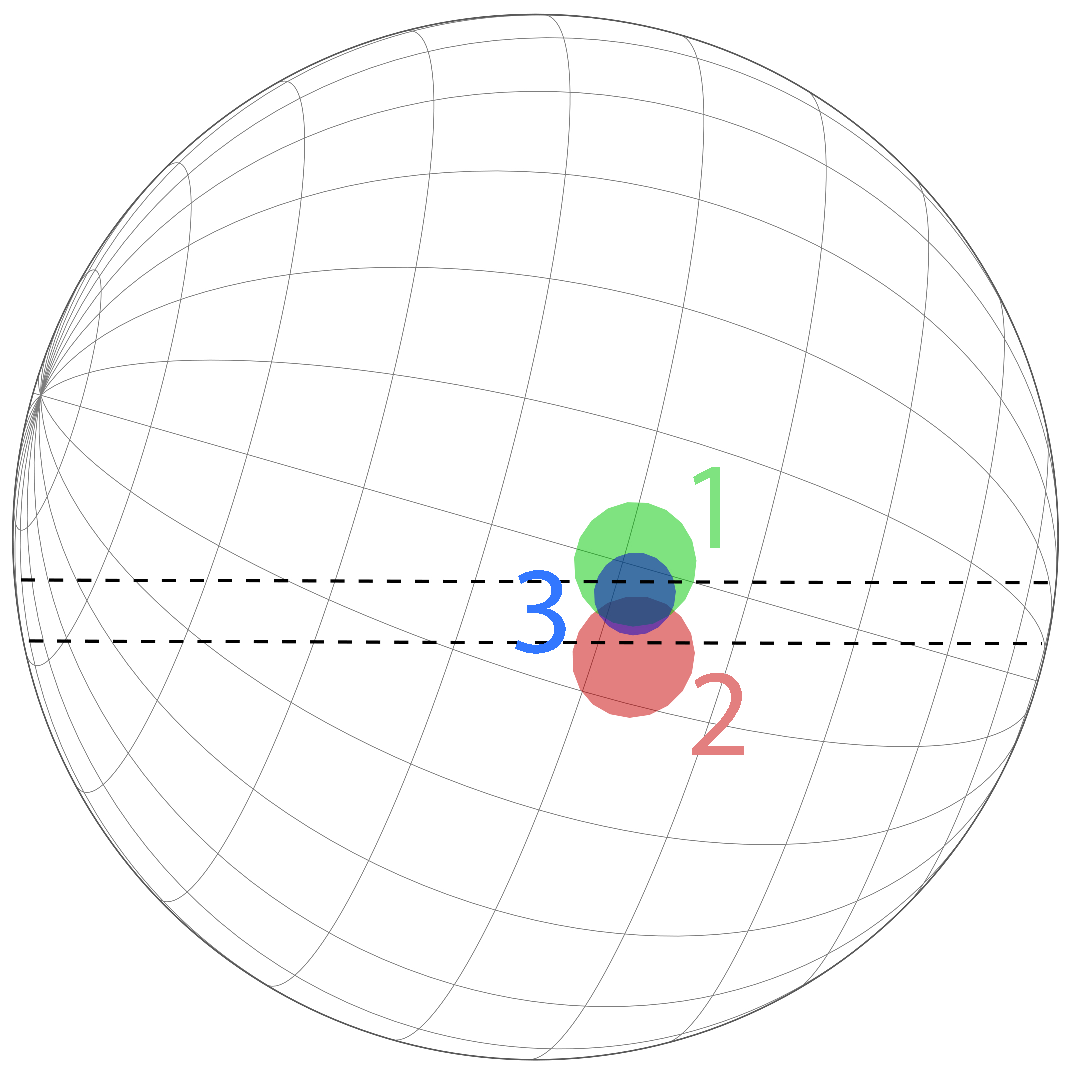
\includegraphics[scale=0.2]{stsp_hat_p_11/spot_degeneracy2.pdf}
\includegraphics[scale=0.45]{stsp_hat_p_11/spot_degeneracy.pdf}
\caption{\textit{Upper}: Map of a few hypothetical spots on HAT-P-11 which would produce similar anomalies in the transit light curve.  The transit chord is bounded by the black dashed lines, the red latitudinal grid mark is the stellar equator -- the stellar rotational pole is tilted into the page and on the right. In this diagram, the planet transits from left to right, from near opposite the rotational pole to near the rotational pole. The ($R_{spot}/R_{star}$, latitude, longitude)  parameters for spot 1 (green), 2 (red), and 3 (blue) are: (0.12, 1.4$^\circ$, 359.8$^\circ$), (0.12, 4.3$^\circ$, 9.8$^\circ$), and (0.08, 2.3$^\circ$, 2.9$^\circ$), respectively. \textit{Lower:} \stsp\ model transits for each spot in the map above. With \kepler's flux precision for HAT-P-11 ($\sim 80$ ppm), these three models would be indistinguishable.}
\label{fig:rp_degeneracy}
\end{figure}

For most transit light curves with spot occultations, there exists a series of spot positions and radii which produce equally good fits to the observations. There are two main degeneracies in our choice of spot model which are critical to understanding the fit results of HAT-P-11; we will call these degeneracies: (1) the transit chord degeneracy and (2) the radius-position degeneracy. 

The transit chord degeneracy is a simple consequence of symmetry. For any small spot placed near the transit chord, a spot of the same radius could be placed on the opposite side of the transit chord (at the same distance from the transit chord) to create an identical bump in the light curve. See for example spots 1 and 2 in Figure~\ref{fig:rp_degeneracy}. 

The transit chord degeneracy may be broken in two scenarios: (1) for some star-planet systems with large impact parameters, the spots would be significantly more foreshortened on one side of the transit chord than the other; or (2) large spots that subtend large angles from the center of the stellar disk to the limb will be more foreshortened near the limb than at disk center, producing asymmetries between spot-crossing ingress and egress. HAT-P-11 has impact parameter $b = 0.141$ so spots projected onto either side of the transit chord will appear roughly symmetric, and therefore the spot position solutions most often come in pairs that are symmetric about the transit chord. However, there are a few exceptionally large spots that give rise to asymmetric spot crossings, which allows the model to select a spot position on only one side of the transit chord.

The radius-position degeneracy arises from trade-off in spot occultation amplitude between spot size and position. A large spot which grazes the edge of the transit chord will produce a bump in the transit light curve similar to a much smaller spot laying within the transit chord. See for example spots 1 and 3 in Figure~\ref{fig:rp_degeneracy}. 

The radius-position degeneracy can be broken with observations at infinite time resolution and flux precision. In the \kepler\ observations of HAT-P-11, the one minute cadence and the single measurement uncertainty $\sigma_{\Delta F / F} \sim 80$ ppm prevent us from distinguishing between small spots near to the transit chord and somewhat larger spots farther from the transit chord. 

More details about \stsp\ model parameter degeneracies are discussed in \citet{Hebb2017}. Examples of \stsp\ fits to the HAT-P-11 light curves and the effects of these degeneracies are discussed in detail in the following section.

\subsection{Examples of degeneracies in results}


\begin{figure}
\centering
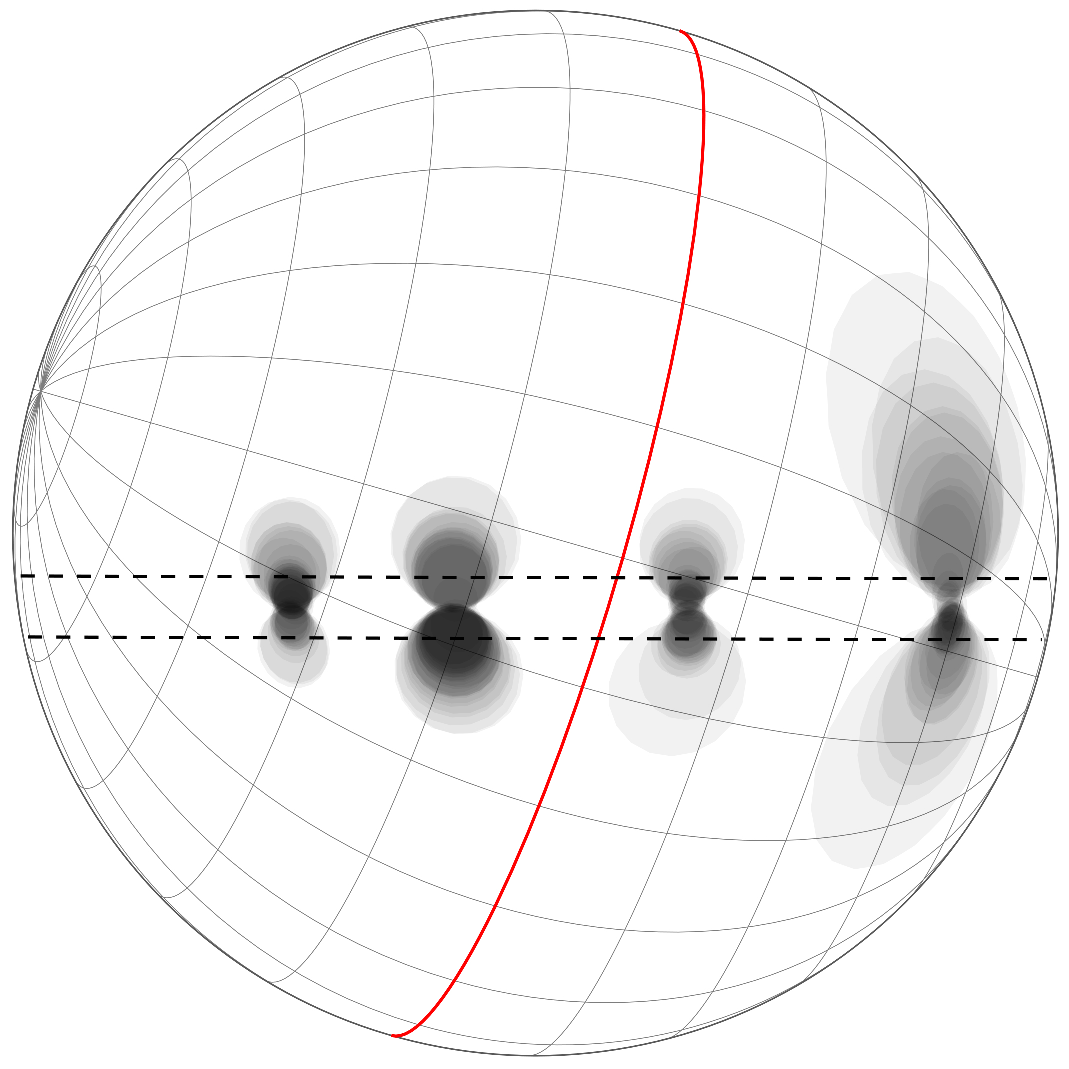
\includegraphics[scale=0.2]{stsp_hat_p_11/transit063.pdf}
\includegraphics[scale=0.45]{stsp_hat_p_11/lc_063.pdf}
\caption{\textit{Lower:} an example transit light curve of HAT-P-11 b (black points) with the maximum likelihood \stsp\ model (red curve). \textit{Upper}: a few random draws from the posterior samples for the spot positions and radii. These four spots are highlighted in blue on the spot map in Figure~\ref{fig:map}.}
\label{fig:transit_063}
\end{figure}

\begin{figure}
\centering
\includegraphics[scale=0.45]{stsp_hat_p_11/063_spot1_rll.pdf}
\caption{Correlations between posterior samples for latitude, longitude and spot radius for the spot second from the left in the graphic in Figure~\ref{fig:transit_063}. The vertical/horizontal black lines mark the maximum likelihood values from the Markov chains. For the analysis of the spot latitude and radius distributions, we use the maximum likelihood values to compute the spotted area in the transit chord, for example, which selects one of the two possible groups of solutions for each spot. Note that the model constrains the minimum spot radius for this spot despite the position-radius degeneracy, which is a result of fixing the spot contrast.}
\label{fig:corner_063}
\end{figure}

We can begin to understand the spot radius-position degeneracy which affects the radius distribution by inspecting the transit on April 18, 2010; see Figures~\ref{fig:transit_063}  and \ref{fig:corner_063}. There are four spot occultations visible in the transit light curve, so we seed the \stsp\ model with four spots, and optimize for the latitude, longitude and radius of each spot with fixed flux contrast ($c=0.3$, as defined in Equation~\ref{eqn:contrast}). The posterior samples for latitude, longitude and radius of each spot cluster into two groups of solutions -- one on each side of the transit chord. In some spot occultations, asymmetry in the photometry produces a preferred solution on one side of the transit chord. In the case of the spot posteriors shown in Figure~\ref{fig:corner_063} (see also the light curve and spot geometry in Figure~\ref{fig:transit_063}), the latitude and longitude have bimodal solutions. Therefore, rather than adopting the mean of these bimodal posteriors as the best solution, we use the parameter values at the maximum likelihood step of the MCMC chains to study spot radii (and latitudes).

For a fixed spot contrast, the radius-position degeneracy biases us towards larger radii. The asymmetry towards large radii can be seen in the bottom left plot of Figure~\ref{fig:corner_063}. If the spot contrast cannot vary, there exists a minimum spot radius which is capable of reproducing the observed occultation amplitude for a direct spot occultation (impact parameter $b=0$). Any indirect or grazing occultations ($b \neq 0$) would require a larger spot to produce the same occultation amplitude, producing an abundance of possible solutions with large spots, centered farther away from the transit chord. For this reason, we do not assert that any spots on HAT-P-11 are certainly larger than the largest sunspot, though the maximum likelihood solutions suggest such spots exist (more on spot radii in Section~\ref{sec:radii}).

\begin{figure}
\centering
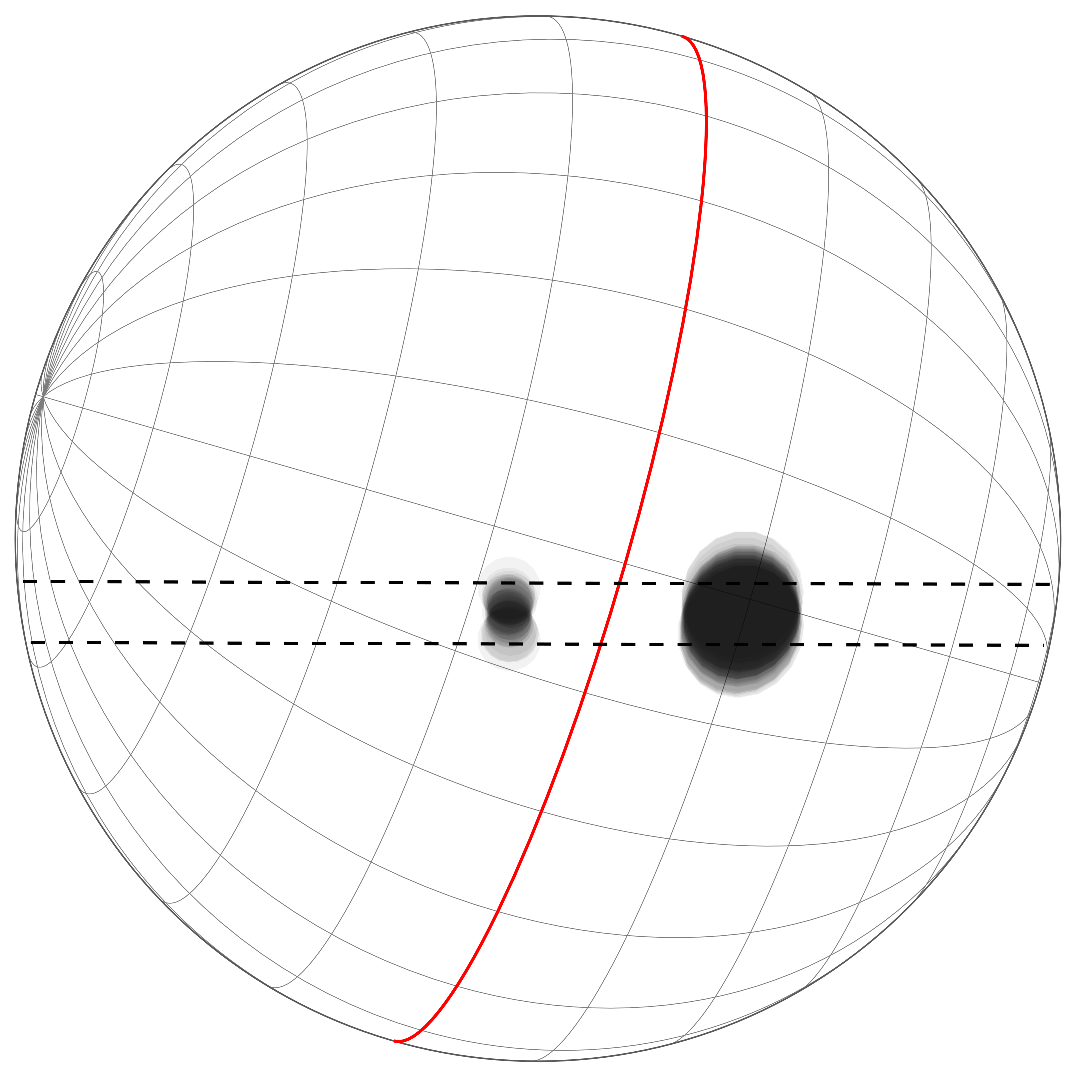
\includegraphics[scale=0.2]{stsp_hat_p_11/transit044.pdf}
\includegraphics[scale=0.4]{stsp_hat_p_11/lc_044.pdf}
\caption{\textit{Lower:} an example transit light curve of HAT-P-11 b (black points) with the maximum likelihood \stsp\ model (red curve). \textit{Upper}: a few random draws from the posterior samples for the spot positions and radii. The transit chord is bounded by the black dashed lines, the red latitudinal grid mark is the stellar equator -- the stellar rotational pole is tilted into the page and on the right. In this diagram, the planet transits from left to right, from near opposite the rotational pole to near the rotational pole. The grid lines are separated by 15$^\circ$, so the active latitudes appear near the grid lines on either side of the equator. Note that the flat-topped spot occultation model light curve corresponds to a spot that must appear to be wider than the transit chord -- setting a constraint on the minimum radius of the spot. The observed fluxes are higher than the model near the mid-occultation time, which is suggestive of a higher spot contrast near the center of the spot. These two spots are highlighted in red on the spot map in Figure~\ref{fig:map}. In physical units, these spots have radii of $22400^{+4000}_{-300}$ and $63700^{+3000}_{-200}$ km.}
\label{fig:transit_044}
\end{figure}


Figure~\ref{fig:transit_044} shows an example light curve model and a few draws from the spot parameter posteriors for the transit on December 31, 2009 UTC. The model of the second spot occultation in this transit has a flat top, and an amplitude similar to $\Delta F/ \delta \sim c = 0.3$, which implies that the spot was occulted with a small impact parameter, and that the spot radius was larger than the planet radius. The geometry of this eclipse parallels planetary transits with negligible limb-darkening, which produce a ``u''-shaped eclipse with a flat bottom. We note that the \kepler\ fluxes at the peak of the second spot occultation have a net positive scatter. This could imply that a more extreme spot contrast is justified at the center of the spot ($c<0.3$), where one might expect the umbra to be. The duration of the flat-topped spot occultation is proportional to the diameter of the spot, so the position and size of this spot are relatively well-constrained by the photometry. This is reflected by the uniformity of the posterior samples of the second spot in Figure~\ref{fig:transit_044} compared to the earlier grazing spot occultation, which is less constrained. The inverted ``v''-shape of the first spot occultation implies that the planet either grazed the spot at high impact parameter -- similar to planetary transits or binary eclipses with high impact parameters, which produce ``v''-shaped eclipses -- or that the spot is similar in size to the size of the planet. As you can see in the samples from the posteriors on the map in Figure~ \ref{fig:transit_044}, the model tends towards a spot centered in the transit chord, slightly smaller than the planet. 



\section{\stsp\ Results} \label{sec:results}
\subsection{Spot Map of HAT-P-11}

\begin{figure*}
\centering
% \includegraphics[scale=0.3]{map_friedrich.pdf}
%\includegraphics[scale=0.58]{map_stsp.pdf}
\includegraphics[scale=0.58]{stsp_hat_p_11/map_stsp.pdf}
\caption{Spots detected on HAT-P-11 with \stsp\ (see Section~\ref{sec:stsp}). The radius of each circle corresponds to the size of the spot. The shading beneath corresponds to the number of times the planet occulted that spatial bin on the stellar surface, which can be used as a proxy for relative completeness. Note that the spots occur preferentially at two active latitudes near $\pm15^\circ$. The 6:1 period commensurability between the orbital period and stellar rotation period produces the alternating longitudinal stripes in relative occultation number. The two red circles in the western hemisphere near longitude $-90^\circ$ highlight the spots derived from the transit light curve in Figure~\ref{fig:transit_044}, and the four blue circles in the eastern hemisphere near longitude $30^\circ$ correspond to the spots derived from the transit light curve in Figure~\ref{fig:transit_063}. The green circle near longitude $-100^\circ$ corresponds to the large spot discussed in Figure~\ref{fig:transit_071}.}
\label{fig:map}
\end{figure*}

We map the maximum-likelihood starspot positions for all 138 transits in Figure~\ref{fig:map}. The circles represent the positions and sizes of the spots inferred with \stsp. The shading of the map corresponds to the number of times the center of the planet occulted each location on the star, which is a proxy for completeness of the spot map -- darker regions were occulted more often. We choose to plot the maximum-likelihood spot positions and radii rather than the means of the posterior samples, because degeneracies between the model parameters can produce bimodal posterior distributions (see Section~\ref{sec:stsp} for discussion on model degeneracies).

The spin-orbit misalignment and spin-orbit commensurability of this system lead to highly inhomogeneous sampling in longitude, so an investigation into the true spot longitude distribution is beyond the scope of this work. However, asymmetries in spot latitude are detectible and readily visible in the spot map in Figure~\ref{fig:map}. The spots are distributed into two active latitudes near $\pm 16^\circ$ latitude, and the northern hemisphere appears to have more spots than the southern hemisphere. We investigate the latitude distribution of spots in the next section.

The transit chord of HAT-P-11 b is inclined $16^\circ$ from perpendicular to the stellar equator -- refer back to Figure~\ref{fig:schematic} for a schematic of the orientation. As a result of this slight misalignment from perpendicular, the planet never occults either pole of the star. It is possible that there are spots at latitudes $\ge 60^\circ$, which have been produced in simulations of highly-active sun-like stars \citep[e.g.][]{Schrijver2001}. Our spot map from transit photometry is insensitive to polar or high latitude spots. 

\subsection{Latitude Distribution} \label{sec:lat_dist}

\begin{figure}
\centering
\includegraphics[scale=0.48]{stsp_hat_p_11/asymmetric_latitudes.pdf}
\caption{Distribution of spot latitudes over four years of observations for both HAT-P-11 and the Sun. The four years of solar observations correspond to the maximum of solar Cycle 19 as observed by \citet{Howard1984}. The HAT-P-11 spot latitudes and their uncertainties are taken from the best-fit solutions from the \stsp\ spot occultation model. Both stars have active latitudes centered on $\pm 16^\circ$ with standard deviations of $\sim 8^\circ$. We put these latitude distributions in context throughout the solar activity cycle in Figure~\ref{fig:sun_vs_hat11}. Though HAT-P-11's hemispheric spot number asymmetry is greater than the Sun's in this particular bin of solar observations, we find that the asymmetry on HAT-P-11 is within the range observed on the Sun; see Section~\ref{sec:lat_dist} for details.}
\label{fig:latitude_model}
\end{figure}

\begin{figure}
\centering
\includegraphics[scale=0.6]{stsp_hat_p_11/sun_vs_hat11.pdf}
\caption{Latitude distributions of sunspots and spots on HAT-P-11, parameterized by the mean latitude of spots in each hemisphere and the standard deviation of spot latitudes in each hemisphere. The circles are the best-fit parameters for four-year bins of the Mt.~Wilson sunspot catalog \citep{Howard1984}. The squares are fits to the HAT-P-11 latitude distribution over the four years of \kepler\ data. The colors of the solar circles represent the number of sunspots in each bin, which is a good proxy for phase of the solar activity cycle (darker points are nearer to solar maximum). Some of the fits have large uncertainties even with many spots, because the latitude distributions are not always well-approximated by Gaussians. The solar measurement closest to HAT-P-11's corresponds to the period 1957-1961 during solar Cycle 19, which is plotted in Figure~\ref{fig:latitude_model} for comparison to HAT-P-11.}
\label{fig:sun_vs_hat11}
\end{figure}

The mean latitudes of sunspots and the widths of their distributions across each hemisphere undergo an $\sim 11$ year cycle, which gives rise to the ``butterfly diagram'' of latitudinal spot density as a function of time \citep[see for example][]{Hathaway2011, Hathaway2015}. Near solar minimum, there are very few sunspots. Spots begin to appear at ``high'' latitudes $\left | \ell \right |  \sim 25^\circ$, and the mean spot latitude drifts towards the equator throughout the cycle, with the maximum number of spots occurring near $\left | \ell \right | \sim 15^\circ$. The northern and southern hemispheres of the Sun can have asymmetric numbers of spots, flares, and other activity indicators \citep[see for example][]{Newton1955, Vizoso1990, Carbonell1993, Li2002}.

To compare the activity of HAT-P-11 to solar activity, we characterize the Sun's spot latitude distribution in the 1917-1985 sunspot catalog from Mt.~Wilson Observatory published by \citet{Howard1984}. We group the solar spot observations into four-year bins similar to the \kepler\ time series of HAT-P-11. On these timescales, the spot latitude distributions on both stars are often similar to Gaussians (see Figure~\ref{fig:latitude_model}), though sometimes the deviations from Gaussians are significant.

We construct a probabilistic model to describe the latitude distributions of spots on HAT-P-11 and on the Sun, following the description of the Gaussian mixture model in Section~\ref{sec:i_s}. We fit for the amplitude, mean, and variance of Gaussians representing the latitude distributions of spots in each hemisphere. We focus on fitting the shape of the latitude distribution and do not compare the total number of spots observed on the two stars to each other, since a correction for the sensitivities and biases of the different observing methods is beyond the scope of this paper.

The latitude distribution of spots of HAT-P-11 and four years of solar observations are shown in Figure~\ref{fig:latitude_model}. The four-year span of solar observations closely resembles the mean spot latitudes and standard deviation of spot latitudes that we measure for HAT-P-11. The sunspots included in Figure~\ref{fig:latitude_model} span the active maximum of solar Cycle 19, which was the solar maximum with the largest recorded number of spots since telescopic observations began \citep{Solanki2013}.

The properties of the maximum-likelihood Gaussian mixture models for HAT-P-11 and the Sun are shown in Figure~\ref{fig:sun_vs_hat11}. The circles show the mean latitudes of spots on each hemisphere of the Sun, and the standard deviations of the spot distributions. The pattern of the solar activity cycle is visible --- sunspots in the beginning of the cycle appear in small numbers at high latitudes, then large numbers near $15^\circ$, before settling back to lower numbers near the equator. The standard deviations of the spot distributions are correlated with the mean latitude --- the active latitudes are broadest at the beginning of the activity cycle when spots form at high latitudes, and the active latitudes become narrower as they approach the equator later in the activity cycle. The combined effect of the shrinking standard deviations with declining mean latitudes produces the ``wings'' in the butterfly diagram.

The distribution of spots on HAT-P-11 sits near the region of $\bar{\ell} - \sigma$ space corresponding to solar maximum. The most similar four-year bin of sunspots, which is roughly consistent with the HAT-P-11 spot distribution in terms of $\bar{\ell}$ and $\bar{\sigma}$, is the bin plotted in Figure~\ref{fig:latitude_model}. The mean active latitudes on HAT-P-11, $\ell = 16 \pm 1^\circ$, correponds to the mean latitudes of sunspots near most solar maxima.

The number of spots observed in each hemisphere is rather asymmetric, but within the range of observed asymmetries on the Sun. Hemispheric asymmetries of the solar spot distribution are often quantified by $(N-S)/(N+S)$, where $N$ is the spot area in the northern hemisphere and $S$ is the spot area in the southern hemisphere \citep{Waldmeier1971, Carbonell1993}. The maximum likelihood \stsp\ spot latitudes and radii from the entire \kepler\ mission give $(N-S)/(N+S)=0.35$. This asymmetry is within the range observed on the Sun by \citet{Howard1984} when observed in four-year bins, varying from -0.1 to 0.6.

\subsection{Radius distribution} \label{sec:radii}

\begin{figure*}
\centering
\includegraphics[scale=0.75]{stsp_hat_p_11/spot_radii.pdf}
\caption{Maximum likelihood spot radii for HAT-P-11 from \kepler\ spot occultations, and for the Sun from Mt.~Wilson Observatory \citep{Howard1984}. The spot radii are given in physical units on the left panel and in fractions of the stellar radius ($R_{spot}/R_{star}$) and millionths of the observer-facing hemisphere ($\mu$Hem) in the right panel. We adopt the radius of HAT-P-11 from \citet{bakos2010}, $R_{star} = 0.752 R_\odot$. For reference, the largest sunspot measurement we could find in the literature was 6132 $\mu$Hem = $R_{spot} / R_{\odot} = 7.7 \times 10^4$ km. We suspect that a significant fraction of HAT-P-11's spots with very large radii are in fact occultations of multiple spots.}
\label{fig:radii}
\end{figure*}

\begin{figure}
\centering
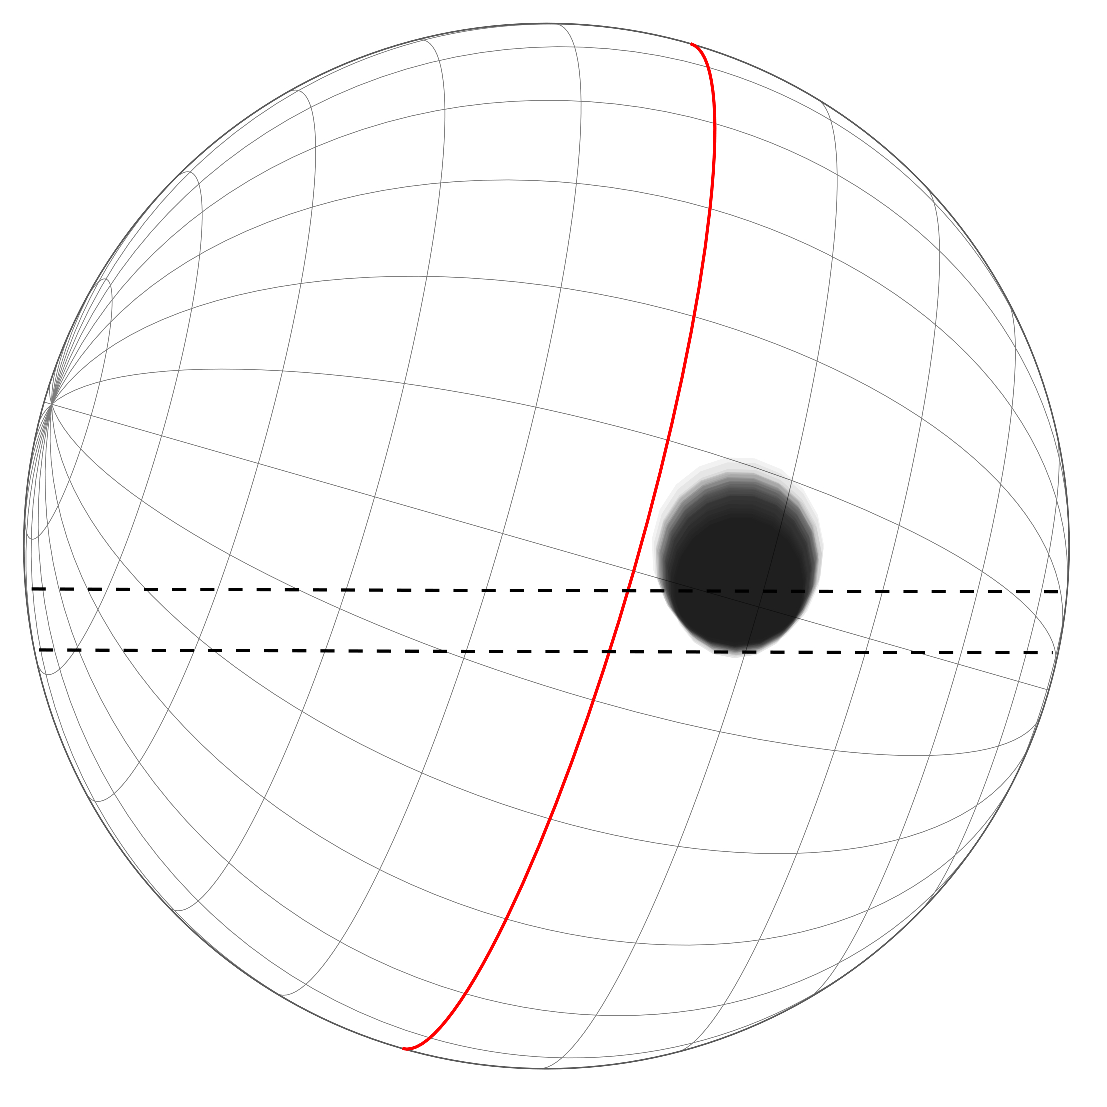
\includegraphics[scale=0.18]{stsp_hat_p_11/transit071.pdf}
\includegraphics[scale=0.35]{stsp_hat_p_11/rad_071.pdf}
\includegraphics[scale=0.45]{stsp_hat_p_11/lc_071.pdf}
\caption{An occultation of a particularly large spot. The maximum likelihood spot radius is $R_{spot}/R_{star} = 0.160_{-0.016}^{+0.007}$, or $84000^{+4000}_{-8000}\pm 6000$ km -- just larger than the largest recorded sunspot (77000 km, \citealt{Newton1955}). This spot is highlighted in green on the spot map in Figure~\ref{fig:map}.}
\label{fig:transit_071}
\end{figure}

We compute the physical spot radius distribution using the radius measurement of HAT-P-11 from \citet{bakos2010}, $R=0.752 \pm 0.021 R_\odot$. The spot radius distribution is shown in Figure~\ref{fig:radii}, along with sunspot radii near activity maximum and minimum. 

The spot radius distribution of HAT-P-11 closely resembles the Sun's at activity maximum for spots with radii $2\times 10^4 < R_{spot} < 5 \times 10^4$ km. 85\% of the spots on HAT-P-11 are smaller than the largest observed sunspot. The HAT-P-11 radius distribution is incomplete for small spots with $R_{spot} \lesssim 2 \times 10^4$ km, since spot occultation amplitudes of those spots are similar in scale to the noise in \kepler\ photometry. The smallest observed sunspots have radii of order $10^3$ km \citep{Solanki2003}, so it is likely that there are also small spots on HAT-P-11 below our S/N threshold.

HAT-P-11's spot distribution has a tail of spots larger than those observed on the Sun, with $R_{spot} > 5 \times 10^4$ km. From visually inspecting the individual transits, it is clear that some of the spots are larger than the largest sunspots. The largest published sunspot measurement that we encountered in the literature was recorded in 1947 by \citet{Newton1955} to have area 6132 $\mu$Hem. We can calculate the radius of a circular spot with this area in units of hemispheres (Hem) by normalizing the area of the circular spot $A_{spot} = \pi R_{spot}^2$ by the area of the observer-facing hemisphere of the star $A_{star} = 2\pi R_{star}^2$,
\begin{equation}
A_{\textrm{Hem}} = \frac{1}{2}\left(\frac{R_{spot}}{R_{star}}\right)^2\\ \\
\frac{R_{spot}}{R_{star}} = \sqrt{2 A_{\textrm{Hem}}}
\end{equation}
Therefore in the circular approximation, the largest reported sunspot had radius $R_{spot}/R_{\odot} = 0.110$ and $R_{spot} \sim 77$ Mm. We can compare that to the spot in Figure~\ref{fig:transit_071}, for example, which has $R_{spot}/R_{star} = 0.160_{-0.016}^{+0.007}$ corresponding to $R_{spot} = 84^{+4}_{-8}$ Mm --- consistent with the largest sunspot. The radius posterior distribution shown in Figure~\ref{fig:transit_071} has a single solution. However, many of these larger spots could be somewhat smaller than the maximum likelihood solution that we are reporting. The spot radius posterior distributions exhibit families of degenerate solutions in which the spot occultation fluxes can be fit equally well by a grazing spot occultation of a large spot or a more direct occultation of a smaller spot (see Section~\ref{sec:degen} for discussion of degeneracies). This could produce a systematic bias towards larger maximum-likelihood spot radii in the values that we report.


\subsection{Spotted area} \label{sec:spotted_area}

\begin{figure}
\centering
\includegraphics[scale=0.6]{stsp_hat_p_11/spotted_area.pdf}
\caption{Spot coverages of HAT-P-11 and the Sun. The HAT-P-11 spotted area is computed the area of the transit chord occulted by spots in the maximum likelihood \stsp\ fit. The spotted areas of the Sun are gathered from the Mt.~Wilson Observatory spot catalog of \citet{Howard1984}, scaled up to account for the areas of penumbra and penumbra, assuming an area ratio of $A_{pen} / A_{umb} = 4$. We have excluded spot coverages for transits that had either no significant spot occultations, or where multiple spot occultations were fit with a single unrealistically large spot, narrowing the sample down to 90 of the 205 transits observed by \kepler.}
\label{fig:spotted_area}
\end{figure}

\begin{table*}
\centering
\begin{tabular}{|lccccccp{3cm}|} 
\hline
Name & Sp. Type & $T_{eff}$ [K] & $P_{rot}$ [d] & $T_{spot}$ [K] & $f_s \, [A_{*/2}]$ & $\left < S \right>$ & Ref. \\ \hline \hline
Sun & G2V & 5777 & 24.47 & 3900-5500 & $0.0003^{+0.0006}_{-0.0001}$ & 0.17 & \citet{Howard1984, Solanki2003, Egeland2017}\\
HAT-P-11 & K4V & 4780 & 29.2 & 4500 (fixed) & $3^{+0.06}_{-0.01}$ & 0.6 & (This work, \citet{bakos2010}) \\
OU Gem  & K3V/K5V & 4925/4550 & 6.991848 & --- & $\le 0.04 - 0.35$ & 0.796 & \citet{ONeal2001, Pace2013} \\
EQ Vir  & K5Ve & 4380 & 3.96 &  $3350 \pm 115$ &$0.33 - 0.45$ & 3.68 & \citet{ONeal2001, Cincunegui2007} \\
XX Tri & K0 III & 4750 & 23.96924 & $3425 \pm 120$ & $0.31 - 0.35$ & -- & \citet{ONeal2004} \\
V833 Tau & K4V & 4500 & 1.7955 & 3175  & 0.51 & 2.460 & \citet{ONeal2004, Pace2013} \\ \hline
\end{tabular}
\caption{Comparison of HAT-P-11, the Sun, and several stars in order of increasing spot coverags ($f_S$, in units of hemispheres [$A_{*/2}$]). The spot temperature range listed for the Sun includes the typical lower limit of umbral temperatures and typical upper limit of penumbral temperatures. The spot temperature of HAT-P-11 is estimated by selecting the PHOENIX model atmosphere that most closely produces a spot contrast of $c=0.3$ in the \kepler\ bandpass \citep{Husser2013}, and should be thought of as the approximate area-weighted spot group temperature in both the umbra and penumbra. The typical solar spot temperature range spans from the coolest regions of the umbra to the hottest regions of the penumbra.}
\label{tab:fillfactors}
\end{table*}

The spot area coverage of the observable hemisphere of a star, or the spot ``filling factor'' $f_S$, has been constrained for several stars with Zeeman-Doppler imaging and molecular band modeling. Since these methods are sensitive to different spot sizes \citep{Solanki2004}, we chose to compare the spots that we detect on HAT-P-11 via photometry with starspots detected via molecular band modeling only. The molecular absorption band spot temperatures and filling factors from \citet{ONeal2001, ONeal2004} are enumerated in Table~\ref{tab:fillfactors}, with spot areas ranging from a few percent to nearly half of the stellar surface. 

We can calculate the spotted area within the transit chord at the maximum-likelihood step in the MCMC chains for each transit. This spotted area measurement is not identical to the spotted area fraction $f_S$ from \citet{ONeal2001, ONeal2004}, which measures the fractional area of spots on the entire observer-facing hemisphere of a star. However, since the transit chord of HAT-P-11 b is nearly perpendicular to the stellar equator, the planet occults most latitudes of the star at one longitude during each transit. Since we expect the distribution of starspots to be azimuthally symmetric -- i.e.~the spot distribution may change as a function of latitude but not longitude -- each transit samples the spotted area of a relatively unbiased slice of the stellar surface. Thus we use the spot coverage within the transit chord as a characteristic spot coverage on the whole star.

In Figure~\ref{fig:spotted_area}, we plot the spotted area within the transit chord for the 138 transits with significant spots modeled by \stsp, compared with the spotted area on the Sun (including both the umbra and penumbra). During the \kepler\ mission, the spotted area on HAT-P-11 varied with mean area coverage $\left< f_{s,H11} \right> = 3^{+6}_{-1} \%$, where the upper and lower error bars are the $84^\textsuperscript{th}$ and $16^\textsuperscript{th}$ percentiles, respectively. We have excluded the transits with no significant spot detections from the above reported $\left< f_{s,H11} \right>$ since the abundance of non-detections is distinct from measurements of zero spotted area; and as we discuss in Section~\ref{sec:spot_number}, the star likely always has large spots facing the observer.

The mode of the solar spot coverage from \citet{Howard1984} is $\left< f_{s,\odot} \right> = 0.0003^{+0.0006}_{-0.0001}$, $\sim$100x smaller than HAT-P-11's. Upper limits on the maximal recorded spotted area of the Sun vary depending on the observations considered, but are typically $\lesssim 0.6\%$ \citep{Balmaceda2009}.

We note that the completeness of spot detections on the Sun is nearly 100\%, whereas on HAT-P-11 we are only sensitive to large spots in the transit chord, which covers about 6\% of the observer-facing hemisphere. Therefore the spot coverage that we report for HAT-P-11 is best treated as a lower limit on the actual spot coverage. With that caveat in mind, HAT-P-11's spot coverage is most similar to the molecular band observations of OU Gem, which varies in the range $f_s \le 0.04$ to $0.35$ \citep{ONeal2001}. 

The high spot coverage of HAT-P-11 compared to the Sun is consistent with its CaII H \& K emission. The Sun's mean $S$-index during Cycle 23 was $\left<S_\odot\right> = 0.1701 \pm 0.0005$ \citep{Egeland2017}, compared to $\left<S_{H11}\right> = 0.61$ for HAT-P-11 \citep{bakos2010}. The solar $S$-index directly correlates with the area coverage by sunspots, so naturally it follows from the high $S$-index that HAT-P-11 should have a higher spot coverage. 

\citet{Shapiro2014} fit for the the relation between sunspot coverage $f_{s,\odot}$ as a function of the solar $S$-index and found:
\begin{equation}
f_{s,\odot}(S) = 0.105 - 1.315 S + 4.102 S^2. \label{eqn:naive}
\end{equation}
If we naively substitute our measured spot coverage $f_{s,H11} \sim 0.03$ for HAT-P-11 into Equation~\ref{eqn:naive}, we predict $\left<S_{H11, pred}\right> \sim 0.26$. The observed $S$-index is much larger --- evidently the activity of Sun-like stars does not scale quadratically with $S$-index in the activity regime relevant to HAT-P-11.

We now revisit the assumption made in Section~\ref{sec:norm} that the maximum flux during each \kepler\ quarter is approximately the unspotted brightness of the star. The spotted area observed on HAT-P-11 is as high as 10\% at times, so the maximum quarterly flux is unlikely to be the unspotted flux of the star. If we are underestimating the unspotted flux of the star, then we will underestimate the transit depth (see Section~\ref{sec:norm}), and therefore underestimate spot occultation amplitudes. This propagates into underestimates of spot radii and underestimates of the spotted area. This bias acts to oppose the bias towards larger spot radii and larger spotted areas discussed in Section~\ref{sec:radii}. Visual inspection of the transit light curve residuals shows that the transit depth is generally consistent with the observations, so we deem that our normalization in Section~\ref{sec:norm} is sufficient.

\subsubsection{Spotted area via flux deficit}

\begin{figure}
\centering
\includegraphics[scale=0.65]{stsp_hat_p_11/flux_deficit.pdf}
\caption{Minimum spot coverage of HAT-P-11, independently inferred from the flux deficits in the out-of-transit portions of the \kepler\ light curve. The minimum spot coverage in the range $0.5$ to $3\%$ is consistent with the spot coverage inferred from the spotted area in the transit chord in the maximum-likelihood \stsp\ models, $f_S = 3^{+6}_{-1} \% $.}
\label{fig:flux_deficit}
\end{figure}

The rotational modulation of the out-of-transit fluxes can independently constrain the spotted area of HAT-P-11 (for an assumed spot contrast). The difference between the brightest and dimmest flux measured in each \kepler\ quarter is equivalent to the product of the fractional projected spotted area and $1-c$, where $c$ is the spot contrast as defined in Equation~\ref{eqn:contrast}. 

In practice, the estimate of the spotted area via the flux deficit is a lower limit on the total spotted area. If there were only a few small spots on the star, the flux deficit would yield the true spot covering fraction. However in the limit of many small spots distributed evenly across the star, each spot that rotates out of view will be replaced by another spot rotating into view, and thus adding more spots would not increase the flux deficit. As we argue in this section and Section~\ref{sec:spot_number}, there are a significant number of spots on the star, and it is unclear if the star is in this saturated flux deficit regime. Thus the spotted area inferred by the flux deficit should be treated as a lower limit on the spotted area.

We compute the fractional spotted area for each \kepler\ quarter from the flux deficit as follows. We mask out all transits, and convolve the fluxes with a Gaussian kernel ($\sigma=50$ fluxes). We normalize each quarter's fluxes by its smoothed maximum flux. The minimum fractional spotted area during each quarter is given by $f_S = \left( 1 - \min\textrm{(flux)} \right)/(1-c)$.

The minimum spotted area inferred by the quarterly flux deficits is shown in Figure~\ref{fig:flux_deficit}. We see that minimum spotted area ranges from 0.1\% to 3\% over the different \kepler\ quarters. This is consistent with the 0.5-10\% spotted area that we infer from modeling spots in the transit chord (Figure~\ref{fig:spotted_area}).  


\subsection{Spot number} \label{sec:spot_number}

During the solar activity cycle, the number of spot groups observed on the Sun at any instant varies from near zero at activity minimum to hundreds at maximum. We measure the number of high-signal spot occultations per transit for HAT-P-11, which we can use to (1) search for evolution in the spot number over time; and (2) to compare to the number of sunspots.

The simplest measurement of the number of starspots that we can obtain from the \kepler\ photometry is the number of spots per transit for all 205 transits. Each transit is short compared to the expected spot evolution timescale (weeks) and the stellar rotation period ($29.2$ d), so each transit gives an instantaneous measurement of the number of spots within the transit chord. These spot numbers of HAT-P-11 are not directly comparable to sunspot numbers because solar observations can resolve much smaller spots than occultation photometry. It is also likely that what appear to be large spots in occultation photometry might really be groups of smaller spots at higher resolution.

We assume that the observed spot count per transit follows a Poisson distribution, and compute the likelihood of detecting the observed spot numbers for a given Poisson rate parameter $\lambda$ (with units of spots detected per transit). We allow the spot count rate to vary as a function of time, as it would throughout the solar activity cycle. We model the number of spots observed per transit with a Poisson distribution $P(\lambda)$ with a linearly varying Poisson rate parameter $\lambda(t) = \lambda_0 (t-t_0) + \lambda_1$, where $\lambda_0$ is the rate of change of the Poisson rate parameter over time (i.e.: how many more/less spots will be counted per year), and $\lambda_1$ is the rate parameter at time $t_0$. We marginalize over the hyperparameters with MCMC and find that the rate parameter slope is $\lambda_0 = 0.12 \pm 0.06$ spots per year. Since this slope is consistent with no slope, we fix $\lambda_0 = 0$ and solve only for a constant rate parameter, and find $\lambda = 0.870 \pm 0.066$ spots per transit.

The apparently constant spot number over four years could be observed for a Sun-like star with period $\sim11$ years if observed near maximum or minimum, or at any phase if the activity cycle has a long period. Spectroscopic activity index measurements over time may distinguish between these two possible cases. 

We can compute a rough estimate of the number of spots on the entire stellar surface by extrapolating from number of spots observed within each transit chord. The occulted fraction of the entire stellar surface area, $A_* = 4\pi R_*^2$, within each transit chord is $\sim 2.9\%$. If we assume there are $\lambda=0.87$ spots per transit from the analysis above, then there are $\sim 30 \pm 2$ spots like the ones detected in transit on the surface of the entire star at any given time, and about $15 \pm 1$ on the observer-facing hemisphere of the star.

We refrain from comparing the number of spots on HAT-P-11 to the common solar spot group number because solar observations are not directly analogous to the \kepler\ photometry. Ground-based observations of the Sun can observe sunspots as small as $R_{spot} = 1750$ km -- well below the smallest spots detected with high confidence on HAT-P-11 via transit photometry. However, we can compare the number of sunspots with radii as large as HAT-P-11's. The turnover in spot frequency for small spots on HAT-P-11 suggests that we are insensitive to spots with $R_{spot,min} < 2 \times 10^4$ km (see Figure~\ref{fig:radii}). We identify 898 spots larger than $2 \times 10^4$ km  observed over 10818 days on the Sun \citep{Howard1984}, which is roughly a rate of $0.08$ spots on the observer-facing hemisphere of the Sun at any instant. On HAT-P-11 we detect 130 such spots in 205 transits. The transit chord of HAT-P-11 b spans 6\% of the observer-facing hemisphere, so we expect roughly 11 spots on HAT-P-11 at any instant with radii $>2 \times 10^4$ km. Clearly there are more spots on HAT-P-11 of this size than on the Sun.

In light of the large spot number of HAT-P-11, and the sunspot-like radii of its spots, we can now interpret the spot area determined in Section~\ref{sec:spotted_area}. The spotted area on HAT-P-11 is 100x greater than solar largely due to the presence of \textit{more} spots, since the spot radii are typically quite similar to large sunspots near solar maximum (see spot radius discussion in Section~\ref{sec:radii}). 

\section{Conclusions and discussion} \label{sec:conclusion}

We have measured the properties of starspots on the active K4 dwarf HAT-P-11 from \kepler\ photometry of its transiting planet. We take advantage of the planet's well known orbital orientation to measure starspot positions during occultations by the planet. The highly misaligned orbit of the planet allows us to unambiguously resolve spot latitudes.

The spots of HAT-P-11 are similar to the Sun's in several ways. The spot contrast is consistent with the area-weighted contrast of typical sunspots, $c=0.3$ (Eqn.~\ref{eqn:contrast}). The mode of the spot radius distribution is similar to the radii of sunspots at solar maximum. The active latitudes of HAT-P-11 have the same mean latitude and standard deviation as the Sun at solar maximum. The asymmetry in the number of spots in each hemisphere is consistent with the range of values observed on the Sun. 

However, the activity of HAT-P-11 is more extreme than the Sun's. The mean spot coverage from 2009-2013 is $3^{+6}_{-1}\%$, $\sim$100x greater than the Sun's. The number of large starspots is roughly 100x greater than the number of similarly sized spots on the Sun. The $S$-index of HAT-P-11 is a factor of two greater than one would expect by extrapolating from the spot coverage--$S$-index relation observed on the Sun.

The similarities between the spot distributions on the Sun and HAT-P-11 are interesting in the context of dynamo theory \citep[e.g.][]{Charbonneau2010}. This K4 star is not fully convective, and therefore is expected to have a tachocline like the Sun. Perhaps the $\alpha\Omega$ dynamo is operating within HAT-P-11 as it does in the Sun. It seems that a $0.8M_\odot$ star with a near-solar rotation rate produces starspots in strikingly similar active latitudes, with more large spots. The theoretical prescriptions for magnetic flux emergence developed for the Sun may therefore be applicable out to spectral type K4 \citep[e.g.][]{Cheung2014}.

Precision spot occultation analysis made possible by \kepler\ could potentially be reproduced with photometry from NASA's TESS mission for HAT-P-11 in particular, and for active planet-host stars in general \citep{Ricker2014}. However, the one-minute cadence photometry was critical for resolving the spot occultation features of HAT-P-11, and time resolution directly translates to latitude resolution for highly misaligned systems. The TESS mission's planned two-minute cadence is likely sufficient to detect spot occultations in systems like HAT-P-11, though shorter cadence ground-based photometry would be preferred.

\subsection{Future Work}

HAT-P-11 is exceptionally bright ($V=9.47$), which makes ground-based observations of spot occultations with amplitudes on the order of 0.1\% feasible. In particular, we plan to collect transit photometry with the holographic diffuser and the ARCTIC imager on the ARC 3.5 m Telescope at the Apache Point Observatory (APO) (Stef\'{a}nsson et al.~2017, submitted). If HAT-P-11 exhibits evolution in the spot latitude distribution like the Sun does, we may be able to observe changes in the mean spot position as the activity cycle progresses. Observing spot occultations from the ground is advantageous because the latitude resolution is linked to the time resolution of the photometry, which can be minimized with large aperture telescopes and thus shorter exposure times compared to \kepler\ or TESS.

The phase of the activity cycle of HAT-P-11 can be constrained over several years by analyzing long-term spectroscopy of the $S$-index. In Morris et al.~(2017, in prep), we constrain the period and amplitude of the activity cycle of HAT-P-11 using archival high resolution spectroscopy of the star, in combination with recent high resolution spectra obtained at APO.

The constraints on the spot coverage of HAT-P-11 from the \kepler\ photometry are complementary to spectroscopic constraints from molecular band modeling. The spot coverage reported here could be independently measured by modeling absorption by TiO and OH in starspots \citep{ONeal2001, ONeal2004}. 

In this work we limited ourselves to studying only the spot occultations in transit to make direct comparisons between spots on HAT-P-11 and sunspots. Simultaneous modeling of the out-of-transit fluxes would provide complementary constraints on the total spot coverage on HAT-P-11. 

% \acknowledgments

% We acknowledge support from NSF grant AST-1312453. We thank Eric Agol, John Lurie, Dan Foreman-Mackey and Charli Sakari for constructive conversations during the development of this work.

% Some of the data presented in this paper were obtained from the Mikulski Archive for Space Telescopes (MAST). STScI is operated by the Association of Universities for Research in Astronomy, Inc., under NASA contract NAS5-26555. Support for MAST for non-HST data is provided by the NASA Office of Space Science via grant NNX09AF08G and by other grants and contracts. This research has made use of NASA's Astrophysics Data System. This work used the Extreme Science and Engineering Discovery Environment (XSEDE), which is supported by National Science Foundation grant number ACI-1548562. This research was done using resources provided by the Open Science Grid [1,2], which is supported by the National Science Foundation award 1148698, and the U.S. Department of Energy's Office of Science. This work was facilitated though the use of advanced computational, storage, and networking infrastructure provided by the Hyak supercomputer system and funded by the STF at the University of Washington.

% \facility{Kepler}

% \software{STSP \citep{Hebb2017}, \texttt{ipython} \citep{ipython}, \texttt{numpy} \citep{VanDerWalt2011}, \texttt{scipy} \citep{scipy},  \texttt{matplotlib} \citep{matplotlib}, \texttt{astropy} \citep{Astropy2013}, \texttt{batman} \citep{Kreidberg2015}, \texttt{gatspy} \citep{gatspy}}

% \appendix

\begin{subappendices}
\section*{Spot contrast} \label{sec:appendix_contrast}

We make some simplifying assumptions to derive constraints on the spot contrast from the amplitudes of spot occultations, and we generalize the formalism later. We will at first calculate the flux only for spot-planet orientations where the planet completely occults the spot or the spot completely encompasses the planet. By ignoring grazing spot occultations, we will calculate maximum spot-occultation amplitudes, since grazing spot occultations yield smaller amplitudes than complete occultations. We also ignore stellar limb darkening.

The flux lost during the transit of a planet with radius $R_p$ across an unspotted star with radius $R_\star$ without limb darkening is
\begin{eqnarray}
\delta_{unspotted} = \frac{\Delta F}{F_\star} = \frac{I_\star \pi R_p^2}{I_\star \pi R_\star^2} = \frac{R_p^2}{R_\star^2}
\end{eqnarray}
where $I_\star$ is the mean surface intensity of the stellar disk per unit area. 
\begin{figure}
\centering
\includegraphics[scale=0.4]{stsp_hat_p_11/contrast_schematic.pdf}
\caption{Schematic for parameter definitions in Section~\ref{sec:contrast}, plotted on the transit of HAT-P-11 b on August 20, 2011 UT. The spot occultation amplitude $A$ is the difference between the flux lost during a transit with no spot occultations and the flux lost during a transit with spot occultations, $A = \delta_{unspotted} - \delta_{spotted}$. Note that in this terminology the ``depth'' $\delta(\mu) = \Delta F(\mu)/F$ is a function of the sky-projected distance between the planet and the star $\mu$, or equivalently time or orbital phase, for a star with limb-darkening.}
\label{fig:contrast_schematic}
\end{figure}

We measure the amplitude of brightening during a spot occultation $A$, see Figure~\ref{fig:contrast_schematic} for a schematic representation. During an occultation of a starspot, the appropriate formula for the observed flux depends on the size of the spot $R_{sp}$ relative to the size of the planet $R_{p}$. If the spot with radius larger than or equal to the radius of the planet $R_{sp} \ge R_p$ and the spot has contrast $c$, the amplitude of the difference in flux between a transit of an unspotted and a spotted star is
\begin{eqnarray}
 A &=& \left. \delta_{unspotted} - \delta_{spotted} \right|_{R_{sp} > R_p} \\
 &=& \frac{I_\star \pi R_p^2}{I_\star \pi R_\star^2} - \frac{((1 - c)I_\star) \pi R_p^2}{ I_\star \pi R_\star^2}\\
A/\delta_{unspotted} &=&  c. \label{eqn:bigspot}
\end{eqnarray}
For a spot smaller than the planet, the difference between the spotted and unspotted flux is
\begin{eqnarray}
 A &=& \left. \delta_{unspotted} - \delta_{spotted} \right|_{R_{sp} < R_p} \\
 &=& \frac{I_\star \pi R_p^2}{I_\star \pi R_\star^2} - \frac{I_\star \pi R_p^2 - c I_\star \pi R_p^2 R_{sp}^2/R_p^2}{ I_\star \pi R_\star^2}\\
 A/\delta_{unspotted} &=&  c \left(\frac{R_{sp}}{R_p}\right)^2
 \label{eqn:littlespot}
\end{eqnarray}

In the small planet limit where $R_p/R_\star \ll 1$, the stellar limb darkening could be defined, for example, with a quadratic law $I(\mu)/I_0 = 1 - u_1(1-\mu) - u_2(1-\mu)^2$, and the instantaneous unspotted depth becomes 
\begin{equation}
\delta_{unspotted}(\mu) =  \frac{R_p^2}{R_\star^2} \left[ \frac{1 - u_1(1-\mu) - u_2(1-\mu)^2}{1 - \frac{1}{3}u_1 - \frac{1}{6}u_2} \right]
\end{equation}
where $\mu$ is the sky-projected distance between the planet and the star. Equations \ref{eqn:bigspot} and \ref{eqn:littlespot} above can be generalized for stars with limb-darkening by replacing $\delta_{unspotted} \rightarrow \delta_{unspotted}(\mu)$.

\end{subappendices}

%\bibliographystyle{apj}
%\bibliography{stsp_hat_p_11/bibliography}

% \bibliography{stsp_hat_p_11/bibliography.bib}
% \begin{thebibliography}{}

% \bibitem[\protect\astroncite{{Astropy Collaboration}
%   et~al.}{2013}]{Astropy2013}
% {Astropy Collaboration}, T.~P. {Robitaille}, E.~J. {Tollerud}, P.~{Greenfield},
%   M.~{Droettboom}, E.~{Bray}, T.~{Aldcroft}, M.~{Davis}, A.~{Ginsburg}, A.~M.
%   {Price-Whelan}, W.~E. {Kerzendorf}, A.~{Conley}, N.~{Crighton}, K.~{Barbary},
%   D.~{Muna}, H.~{Ferguson}, F.~{Grollier}, M.~M. {Parikh}, P.~H. {Nair}, H.~M.
%   {Unther}, C.~{Deil}, J.~{Woillez}, S.~{Conseil}, R.~{Kramer}, J.~E.~H.
%   {Turner}, L.~{Singer}, R.~{Fox}, B.~A. {Weaver}, V.~{Zabalza}, Z.~I.
%   {Edwards}, K.~{Azalee Bostroem}, D.~J. {Burke}, A.~R. {Casey}, S.~M.
%   {Crawford}, N.~{Dencheva}, J.~{Ely}, T.~{Jenness}, K.~{Labrie}, P.~{Lian
%   Lim}, F.~{Pierfederici}, A.~{Pontzen}, A.~{Ptak}, B.~{Refsdal},
%   M.~{Servillat}, and O.~{Streicher}\leavevmode\nopagebreak\newline 2013.
% \newblock {Astropy: A community Python package for astronomy}.
% \newblock {\em \aap}, 558:A33.

% \bibitem[\protect\astroncite{{Babcock}}{1961}]{Babcock1961}
% {Babcock}, H.~W.\leavevmode\nopagebreak\newline 1961.
% \newblock {The Topology of the Sun's Magnetic Field and the 22-YEAR Cycle.}
% \newblock {\em \apj}, 133:572.

% \bibitem[\protect\astroncite{{Bakos} et~al.}{2010}]{bakos2010}
% {Bakos}, G.~{\'A}., G.~{Torres}, A.~{P{\'a}l}, J.~{Hartman}, G.~{Kov{\'a}cs},
%   R.~W. {Noyes}, D.~W. {Latham}, D.~D. {Sasselov}, B.~{Sip{\H o}cz}, G.~A.
%   {Esquerdo}, D.~A. {Fischer}, J.~A. {Johnson}, G.~W. {Marcy}, R.~P. {Butler},
%   H.~{Isaacson}, A.~{Howard}, S.~{Vogt}, G.~{Kov{\'a}cs}, J.~{Fernandez},
%   A.~{Mo{\'o}r}, R.~P. {Stefanik}, J.~{L{\'a}z{\'a}r}, I.~{Papp}, and
%   P.~{S{\'a}ri}\leavevmode\nopagebreak\newline 2010.
% \newblock {HAT-P-11b: A Super-Neptune Planet Transiting a Bright K Star in the
%   Kepler Field}.
% \newblock {\em \apj}, 710:1724--1745.

% \bibitem[\protect\astroncite{{Balmaceda} et~al.}{2009}]{Balmaceda2009}
% {Balmaceda}, L.~A., S.~K. {Solanki}, N.~A. {Krivova}, and
%   S.~{Foster}\leavevmode\newline 2009.
% \newblock {A homogeneous database of sunspot areas covering more than 130
%   years}.
% \newblock {\em Journal of Geophysical Research (Space Physics)}, 114:A07104.

% \bibitem[\protect\astroncite{{B{\'e}ky} et~al.}{2014a}]{Beky2014a}
% {B{\'e}ky}, B., M.~J. {Holman}, D.~M. {Kipping}, and R.~W.
%   {Noyes}\leavevmode\nopagebreak\newline 2014a.
% \newblock {Stellar Rotation-Planetary Orbit Period Commensurability in the
%   HAT-P-11 System}.
% \newblock {\em \apj}, 788:1.

% \bibitem[\protect\astroncite{{B{\'e}ky} et~al.}{2014b}]{Beky2014b}
% {B{\'e}ky}, B., D.~M. {Kipping}, and M.~J.
%   {Holman}\leavevmode\nopagebreak\newline 2014b.
% \newblock {SPOTROD: a semi-analytic model for transits of spotted stars}.
% \newblock {\em \mnras}, 442:3686--3699.

% \bibitem[\protect\astroncite{{Berdyugina}}{2005}]{Berdyugina2005}
% {Berdyugina}, S.~V.\leavevmode\nopagebreak\newline 2005.
% \newblock {Starspots: A Key to the Stellar Dynamo}.
% \newblock {\em Living Reviews in Solar Physics}, 2:8.

% \bibitem[\protect\astroncite{{Carbonell} et~al.}{1993}]{Carbonell1993}
% {Carbonell}, M., R.~{Oliver}, and J.~L.
%   {Ballester}\leavevmode\nopagebreak\newline 1993.
% \newblock {On the asymmetry of solar activity}.
% \newblock {\em \aap}, 274:497.

% \bibitem[\protect\astroncite{{Carter} et~al.}{2011}]{Carter2011}
% {Carter}, J.~A., J.~N. {Winn}, M.~J. {Holman}, D.~{Fabrycky}, Z.~K. {Berta},
%   C.~J. {Burke}, and P.~{Nutzman}\leavevmode\nopagebreak\newline 2011.
% \newblock {The Transit Light Curve Project. XIII. Sixteen Transits of the
%   Super-Earth GJ 1214b}.
% \newblock {\em \apj}, 730:82.

% \bibitem[\protect\astroncite{Charbonneau}{2010}]{Charbonneau2010}
% Charbonneau, P.\leavevmode\nopagebreak\newline 2010.
% \newblock Dynamo models of the solar cycle.
% \newblock {\em Living Reviews in Solar Physics}, 7(1):3.

% \bibitem[\protect\astroncite{Cheung and Isobe}{2014}]{Cheung2014}
% Cheung, M. C.~M. and H.~Isobe\leavevmode\nopagebreak\newline 2014.
% \newblock Flux emergence (theory).
% \newblock {\em Living Reviews in Solar Physics}, 11(1):3.

% \bibitem[\protect\astroncite{{Christensen-Dalsgaard}
%   et~al.}{2010}]{Christensen-Dalsgaard2010}
% {Christensen-Dalsgaard}, J., H.~{Kjeldsen}, T.~M. {Brown}, R.~L. {Gilliland},
%   T.~{Arentoft}, S.~{Frandsen}, P.-O. {Quirion}, W.~J. {Borucki}, D.~{Koch},
%   and J.~M. {Jenkins}\leavevmode\nopagebreak\newline 2010.
% \newblock {Asteroseismic Investigation of Known Planet Hosts in the Kepler
%   Field}.
% \newblock {\em \apjl}, 713:L164--L168.

% \bibitem[\protect\astroncite{{Cincunegui} et~al.}{2007}]{Cincunegui2007}
% {Cincunegui}, C., R.~F. {D{\'{\i}}az}, and P.~J.~D.
%   {Mauas}\leavevmode\nopagebreak\newline 2007.
% \newblock {H{$\alpha$} and the Ca II H and K lines as activity proxies for
%   late-type stars}.
% \newblock {\em \aap}, 469:309--317.

% \bibitem[\protect\astroncite{{Csizmadia} et~al.}{2013}]{Csizmadia2013}
% {Csizmadia}, S., T.~{Pasternacki}, C.~{Dreyer}, J.~{Cabrera}, A.~{Erikson}, and
%   H.~{Rauer}\leavevmode\nopagebreak\newline 2013.
% \newblock {The effect of stellar limb darkening values on the accuracy of the
%   planet radii derived from photometric transit observations}.
% \newblock {\em \aap}, 549:A9.

% \bibitem[\protect\astroncite{{Czesla} et~al.}{2009}]{Czesla2009}
% {Czesla}, S., K.~F. {Huber}, U.~{Wolter}, S.~{Schr{\"o}ter}, and J.~H.~M.~M.
%   {Schmitt}\leavevmode\nopagebreak\newline 2009.
% \newblock {How stellar activity affects the size estimates of extrasolar
%   planets}.
% \newblock {\em \aap}, 505:1277--1282.

% \bibitem[\protect\astroncite{{Deming} et~al.}{2011}]{Deming2011}
% {Deming}, D., P.~V. {Sada}, B.~{Jackson}, S.~W. {Peterson}, E.~{Agol}, H.~A.
%   {Knutson}, D.~E. {Jennings}, F.~{Haase}, and
%   K.~{Bays}\leavevmode\nopagebreak\newline 2011.
% \newblock {Kepler and Ground-based Transits of the Exo-Neptune HAT-P-11b}.
% \newblock {\em \apj}, 740:33.

% \bibitem[\protect\astroncite{{Egeland} et~al.}{2017}]{Egeland2017}
% {Egeland}, R., W.~{Soon}, S.~{Baliunas}, J.~C. {Hall}, A.~A. {Pevtsov}, and
%   L.~{Bertello}\leavevmode\nopagebreak\newline 2017.
% \newblock {The Mount Wilson Observatory S-index of the Sun}.
% \newblock {\em \apj}, 835:25.

% \bibitem[\protect\astroncite{{Fabrycky} and {Winn}}{2009}]{Fabrycky2009}
% {Fabrycky}, D.~C. and J.~N. {Winn}\leavevmode\nopagebreak\newline 2009.
% \newblock {Exoplanetary Spin-Orbit Alignment: Results from the Ensemble of
%   Rossiter-McLaughlin Observations}.
% \newblock {\em \apj}, 696:1230--1240.

% \bibitem[\protect\astroncite{{Foreman-Mackey}
%   et~al.}{2013}]{Foreman-Mackey2013}
% {Foreman-Mackey}, D., D.~W. {Hogg}, D.~{Lang}, and
%   J.~{Goodman}\leavevmode\nopagebreak\newline 2013.
% \newblock {emcee: The MCMC Hammer}.
% \newblock {\em \pasp}, 125:306--312.

% \bibitem[\protect\astroncite{{Goodman} and {Weare}}{2010}]{Goodman2010}
% {Goodman}, J. and J.~{Weare}\leavevmode\nopagebreak\newline 2010.
% \newblock {Ensemble samplers with affine invariance}.
% \newblock {\em Communications in Applied Mathematics and Computational
%   Science}, 5:65--80.

% \bibitem[\protect\astroncite{{Hathaway}}{2011}]{Hathaway2011}
% {Hathaway}, D.~H.\leavevmode\nopagebreak\newline 2011.
% \newblock {A Standard Law for the Equatorward Drift of the Sunspot Zones}.
% \newblock {\em \solphys}, 273:221--230.

% \bibitem[\protect\astroncite{{Hathaway}}{2015}]{Hathaway2015}
% {Hathaway}, D.~H.\leavevmode\nopagebreak\newline 2015.
% \newblock {The Solar Cycle}.
% \newblock {\em Living Reviews in Solar Physics}, 12.

% \bibitem[\protect\astroncite{{Hebb} et~al.}{2017}]{Hebb2017}
% {Hebb}, L., {Rohn}, G., et al.\leavevmode\nopagebreak\newline 2017 (in prep.).
% \newblock {STSP: A starspot occultation model}.

% \bibitem[\protect\astroncite{{Hirano} et~al.}{2011}]{Hirano2011}
% {Hirano}, T., N.~{Narita}, A.~{Shporer}, B.~{Sato}, W.~{Aoki}, and
%   M.~{Tamura}\leavevmode\nopagebreak\newline 2011.
% \newblock {A Possible Tilted Orbit of the Super-Neptune HAT-P-11b}.
% \newblock {\em \pasj}, 63:531--.

% \bibitem[\protect\astroncite{{Howard} et~al.}{1984}]{Howard1984}
% {Howard}, R., P.~I. {Gilman}, and P.~A. {Gilman}\leavevmode\nopagebreak\newline
%   1984.
% \newblock {Rotation of the sun measured from Mount Wilson white-light images}.
% \newblock {\em \apj}, 283:373--384.

% \bibitem[\protect\astroncite{{Hunter}}{2007}]{matplotlib}
% {Hunter}, J.~D.\leavevmode\nopagebreak\newline 2007.
% \newblock {Matplotlib: A 2D Graphics Environment}.
% \newblock {\em Computing in Science and Engineering}, 9:90--95.

% \bibitem[\protect\astroncite{{Husser} et~al.}{2013}]{Husser2013}
% {Husser}, T.-O., S.~{Wende-von Berg}, S.~{Dreizler}, D.~{Homeier},
%   A.~{Reiners}, T.~{Barman}, and P.~H.
%   {Hauschildt}\leavevmode\nopagebreak\newline 2013.
% \newblock {A new extensive library of PHOENIX stellar atmospheres and synthetic
%   spectra}.
% \newblock {\em \aap}, 553:A6.

% \bibitem[\protect\astroncite{Jones et~al.}{01  }]{scipy}
% Jones, E., T.~Oliphant, P.~Peterson, et~al.\leavevmode\nopagebreak\newline
%   2001--.
% \newblock {SciPy}: Open source scientific tools for {Python}.
% \newblock [Online; accessed <today>].

% \bibitem[\protect\astroncite{{Keppens} and {Martinez
%   Pillet}}{1996}]{Keppens1996}
% {Keppens}, R. and V.~{Martinez Pillet}\leavevmode\nopagebreak\newline 1996.
% \newblock {The magnetic structure of pores and sunspots derived from Advanced
%   Stokes Polarimeter data.}
% \newblock {\em \aap}, 316:229--242.

% \bibitem[\protect\astroncite{{Kipping}}{2013}]{Kipping2013}
% {Kipping}, D.~M.\leavevmode\nopagebreak\newline 2013.
% \newblock {Efficient, uninformative sampling of limb darkening coefficients for
%   two-parameter laws}.
% \newblock {\em \mnras}, 435:2152--2160.

% \bibitem[\protect\astroncite{{Kreidberg}}{2015}]{Kreidberg2015}
% {Kreidberg}, L.\leavevmode\nopagebreak\newline 2015.
% \newblock {BATMAN: BAsic Transit Model cAlculatioN in Python}.
% \newblock {\em \pasp}, 127:1161--1165.

% \bibitem[\protect\astroncite{{Leonard} and {Choudhary}}{2008}]{Leonard2008}
% {Leonard}, T. and D.~P. {Choudhary}\leavevmode\nopagebreak\newline 2008.
% \newblock {Intensity and Magnetic Field Distribution of Sunspots}.
% \newblock {\em \solphys}, 252:33--41.

% \bibitem[\protect\astroncite{{Li} et~al.}{2002}]{Li2002}
% {Li}, K.-J., X.-H. {Liu}, H.-S. {Yun}, S.-Y. {Xiong}, H.-F. {Liang}, H.-Z.
%   {Zhao}, L.-S. {Zhan}, and X.-M. {Gu}\leavevmode\nopagebreak\newline 2002.
% \newblock {Asymmetrical Distribution of Sunspot Groups in the Solar
%   Hemispheres}.
% \newblock {\em \pasj}, 54:629--633.

% \bibitem[\protect\astroncite{{Mandel} and {Agol}}{2002}]{Mandel2002}
% {Mandel}, K. and E.~{Agol}\leavevmode\nopagebreak\newline 2002.
% \newblock {Analytic Light Curves for Planetary Transit Searches}.
% \newblock {\em \apjl}, 580:L171--L175.

% \bibitem[\protect\astroncite{{Neff} et~al.}{1995}]{Neff1995}
% {Neff}, J.~E., D.~{O'Neal}, and S.~H. {Saar}\leavevmode\nopagebreak\newline
%   1995.
% \newblock {Absolute Measurements of Starspot Area and Temperature: II Pegasi in
%   1989 October}.
% \newblock {\em \apj}, 452:879.

% \bibitem[\protect\astroncite{{Newton}}{1955}]{Newton1955}
% {Newton}, H.~W.\leavevmode\nopagebreak\newline 1955.
% \newblock {The lineage of the great sunspots}.
% \newblock {\em Vistas in Astronomy}, 1:666--674.

% \bibitem[\protect\astroncite{{Ohta} et~al.}{2005}]{Ohta2005}
% {Ohta}, Y., A.~{Taruya}, and Y.~{Suto}\leavevmode\nopagebreak\newline 2005.
% \newblock {The Rossiter-McLaughlin Effect and Analytic Radial Velocity Curves
%   for Transiting Extrasolar Planetary Systems}.
% \newblock {\em \apj}, 622:1118--1135.

% \bibitem[\protect\astroncite{{O'Neal} et~al.}{2004}]{ONeal2004}
% {O'Neal}, D., J.~E. {Neff}, S.~H. {Saar}, and
%   M.~{Cuntz}\leavevmode\nopagebreak\newline 2004.
% \newblock {Further Results of TiO-Band Observations of Starspots}.
% \newblock {\em \aj}, 128:1802--1811.

% \bibitem[\protect\astroncite{{O'Neal} et~al.}{2001}]{ONeal2001}
% {O'Neal}, D., J.~E. {Neff}, S.~H. {Saar}, and J.~K.
%   {Mines}\leavevmode\nopagebreak\newline 2001.
% \newblock {Hydroxyl 1.563 Micron Absorption from Starspots on Active Stars}.
% \newblock {\em \aj}, 122:1954--1964.

% \bibitem[\protect\astroncite{{O'Neal} et~al.}{1996}]{ONeal1996}
% {O'Neal}, D., S.~H. {Saar}, and J.~E. {Neff}\leavevmode\nopagebreak\newline
%   1996.
% \newblock {Measurements of Starspot Area and Temperature on Five Active,
%   Evolved Stars}.
% \newblock {\em \apj}, 463:766.

% \bibitem[\protect\astroncite{{Pace}}{2013}]{Pace2013}
% {Pace}, G.\leavevmode\nopagebreak\newline 2013.
% \newblock {Chromospheric activity as age indicator. An L-shaped
%   chromospheric-activity versus age diagram}.
% \newblock {\em \aap}, 551:L8.

% \bibitem[\protect\astroncite{{Parker}}{1955a}]{Parker1955b}
% {Parker}, E.~N.\leavevmode\nopagebreak\newline 1955a.
% \newblock {Hydromagnetic Dynamo Models.}
% \newblock {\em \apj}, 122:293.

% \bibitem[\protect\astroncite{{Parker}}{1955b}]{Parker1955a}
% {Parker}, E.~N.\leavevmode\nopagebreak\newline 1955b.
% \newblock {The Formation of Sunspots from the Solar Toroidal Field.}
% \newblock {\em \apj}, 121:491.

% \bibitem[\protect\astroncite{Perez and Granger}{2007}]{ipython}
% Perez, F. and B.~E. Granger\leavevmode\nopagebreak\newline 2007.
% \newblock Ipython: A system for interactive scientific computing.
% \newblock {\em Computing in Science and Engg.}, 9(3):21--29.

% \bibitem[\protect\astroncite{{Petit} et~al.}{2008}]{Petit2008}
% {Petit}, P., B.~{Dintrans}, S.~K. {Solanki}, J.-F. {Donati}, M.~{Auri{\`e}re},
%   F.~{Ligni{\`e}res}, J.~{Morin}, F.~{Paletou}, J.~{Ramirez Velez},
%   C.~{Catala}, and R.~{Fares}\leavevmode\nopagebreak\newline 2008.
% \newblock {Toroidal versus poloidal magnetic fields in Sun-like stars: a
%   rotation threshold}.
% \newblock {\em \mnras}, 388:80--88.

% \bibitem[\protect\astroncite{Pordes et~al.}{2007}]{osg}
% Pordes, R., D.~Petravick, B.~Kramer, D.~Olson, M.~Livny, A.~Roy, P.~Avery,
%   K.~Blackburn, T.~Wenaus, F.~Würthwein, I.~Foster, R.~Gardner, M.~Wilde,
%   A.~Blatecky, J.~McGee, and R.~Quick\leavevmode\nopagebreak\newline 2007.
% \newblock The open science grid.
% \newblock {\em Journal of Physics: Conference Series}, 78(1):012057.

% \bibitem[\protect\astroncite{{Reiners}}{2012}]{Reiners2012}
% {Reiners}, A.\leavevmode\nopagebreak\newline 2012.
% \newblock {Observations of Cool-Star Magnetic Fields}.
% \newblock {\em Living Reviews in Solar Physics}, 9:1.

% \bibitem[\protect\astroncite{{Ricker} et~al.}{2014}]{Ricker2014}
% {Ricker}, G.~R., J.~N. {Winn}, R.~{Vanderspek}, D.~W. {Latham}, G.~{\'A}.
%   {Bakos}, J.~L. {Bean}, Z.~K. {Berta-Thompson}, T.~M. {Brown}, L.~{Buchhave},
%   N.~R. {Butler}, R.~P. {Butler}, W.~J. {Chaplin}, D.~{Charbonneau},
%   J.~{Christensen-Dalsgaard}, M.~{Clampin}, D.~{Deming}, J.~{Doty}, N.~{De
%   Lee}, C.~{Dressing}, E.~W. {Dunham}, M.~{Endl}, F.~{Fressin}, J.~{Ge},
%   T.~{Henning}, M.~J. {Holman}, A.~W. {Howard}, S.~{Ida}, J.~{Jenkins},
%   G.~{Jernigan}, J.~A. {Johnson}, L.~{Kaltenegger}, N.~{Kawai}, H.~{Kjeldsen},
%   G.~{Laughlin}, A.~M. {Levine}, D.~{Lin}, J.~J. {Lissauer}, P.~{MacQueen},
%   G.~{Marcy}, P.~R. {McCullough}, T.~D. {Morton}, N.~{Narita}, M.~{Paegert},
%   E.~{Palle}, F.~{Pepe}, J.~{Pepper}, A.~{Quirrenbach}, S.~A. {Rinehart},
%   D.~{Sasselov}, B.~{Sato}, S.~{Seager}, A.~{Sozzetti}, K.~G. {Stassun},
%   P.~{Sullivan}, A.~{Szentgyorgyi}, G.~{Torres}, S.~{Udry}, and
%   J.~{Villasenor}\leavevmode\nopagebreak\newline 2014.
% \newblock {Transiting Exoplanet Survey Satellite (TESS)}.
% \newblock In {\em Space Telescopes and Instrumentation 2014: Optical, Infrared,
%   and Millimeter Wave}, volume 9143 of {\em \procspie}, P.~ 914320.

% \bibitem[\protect\astroncite{{Saar}}{1990}]{Saar1990}
% {Saar}, S.~H.\leavevmode\nopagebreak\newline 1990.
% \newblock {Magnetic Fields on Solar-like Stars: The First Decade}.
% \newblock In {\em Solar Photosphere: Structure, Convection, and Magnetic
%   Fields}, J.~O. {Stenflo}, ed., volume 138 of {\em IAU Symposium}, Pp.~
%   427--441.

% \bibitem[\protect\astroncite{{Sanchis-Ojeda} and
%   {Winn}}{2011}]{Sanchis-Ojeda2011}
% {Sanchis-Ojeda}, R. and J.~N. {Winn}\leavevmode\nopagebreak\newline 2011.
% \newblock {Starspots, Spin-Orbit Misalignment, and Active Latitudes in the
%   HAT-P-11 Exoplanetary System}.
% \newblock {\em \apj}, 743:61.

% \bibitem[\protect\astroncite{{Schrijver} and {Title}}{2001}]{Schrijver2001}
% {Schrijver}, C.~J. and A.~M. {Title}\leavevmode\nopagebreak\newline 2001.
% \newblock {On the Formation of Polar Spots in Sun-like Stars}.
% \newblock {\em \apj}, 551:1099--1106.

% \bibitem[\protect\astroncite{{Shapiro} et~al.}{2014}]{Shapiro2014}
% {Shapiro}, A.~I., S.~K. {Solanki}, N.~A. {Krivova}, W.~K. {Schmutz}, W.~T.
%   {Ball}, R.~{Knaack}, E.~V. {Rozanov}, and Y.~C.
%   {Unruh}\leavevmode\nopagebreak\newline 2014.
% \newblock {Variability of Sun-like stars: reproducing observed photometric
%   trends}.
% \newblock {\em \aap}, 569:A38.

% \bibitem[\protect\astroncite{{Solanki}}{2003}]{Solanki2003}
% {Solanki}, S.~K.\leavevmode\nopagebreak\newline 2003.
% \newblock {Sunspots: An overview}.
% \newblock {\em \aapr}, 11:153--286.

% \bibitem[\protect\astroncite{{Solanki} et~al.}{2013}]{Solanki2013}
% {Solanki}, S.~K., N.~A. {Krivova}, and J.~D.
%   {Haigh}\leavevmode\nopagebreak\newline 2013.
% \newblock {Solar Irradiance Variability and Climate}.
% \newblock {\em \araa}, 51:311--351.

% \bibitem[\protect\astroncite{{Solanki} and {Unruh}}{2004}]{Solanki2004}
% {Solanki}, S.~K. and Y.~C. {Unruh}\leavevmode\nopagebreak\newline 2004.
% \newblock {Spot sizes on Sun-like stars}.
% \newblock {\em \mnras}, 348:307--315.

% \bibitem[\protect\astroncite{{Southworth}}{2011}]{Southworth2011}
% {Southworth}, J.\leavevmode\nopagebreak\newline 2011.
% \newblock {Homogeneous studies of transiting extrasolar planets - IV. Thirty
%   systems with space-based light curves}.
% \newblock {\em \mnras}, 417:2166--2196.

% \bibitem[\protect\astroncite{Towns et~al.}{2014}]{xsede}
% Towns, J., T.~Cockerill, M.~Dahan, I.~Foster, K.~Gaither, A.~Grimshaw,
%   V.~Hazlewood, S.~Lathrop, D.~Lifka, G.~D. Peterson, R.~Roskies, J.~R. Scott,
%   and N.~Wilkins-Diehr\leavevmode\nopagebreak\newline 2014.
% \newblock Xsede: Accelerating scientific discovery.
% \newblock {\em Computing in Science \& Engineering}, 16(5):62--74.

% \bibitem[\protect\astroncite{{Van Der Walt} et~al.}{2011}]{VanDerWalt2011}
% {Van Der Walt}, S., S.~C. {Colbert}, and
%   G.~{Varoquaux}\leavevmode\nopagebreak\newline 2011.
% \newblock {The NumPy array: a structure for efficient numerical computation}.
% \newblock {\em ArXiv e-prints}.

% \bibitem[\protect\astroncite{Vanderplas}{2015}]{gatspy}
% Vanderplas, J.\leavevmode\nopagebreak\newline 2015.
% \newblock {gatspy: General tools for Astronomical Time Series in Python}.

% \bibitem[\protect\astroncite{{Vizoso} and {Ballester}}{1990}]{Vizoso1990}
% {Vizoso}, G. and J.~L. {Ballester}\leavevmode\nopagebreak\newline 1990.
% \newblock {The north-south asymmetry of sunspots}.
% \newblock {\em \aap}, 229:540--546.

% \bibitem[\protect\astroncite{{Waldmeier}}{1971}]{Waldmeier1971}
% {Waldmeier}, M.\leavevmode\nopagebreak\newline 1971.
% \newblock {The asymmetry of solar activity in the years 1959 1969}.
% \newblock {\em \solphys}, 20:332--344.

% \bibitem[\protect\astroncite{{Winn} et~al.}{2010}]{Winn2010}
% {Winn}, J.~N., J.~A. {Johnson}, A.~W. {Howard}, G.~W. {Marcy}, H.~{Isaacson},
%   A.~{Shporer}, G.~{\'A}. {Bakos}, J.~D. {Hartman}, and
%   S.~{Albrecht}\leavevmode\nopagebreak\newline 2010.
% \newblock {The Oblique Orbit of the Super-Neptune HAT-P-11b}.
% \newblock {\em \apjl}, 723:L223--L227.

% \end{thebibliography}

% \end{document}


\chapter{The Chromospheric Activity of HAT-P-11: an Unusually Active, Planet-hosting K Dwarf} \label{chap:h11sindex}

In the previous chapter, we opened a window into the stellar magnetic activity of the K4 dwarf HAT-P-11 using its transiting exoplanet. We found that HAT-P-11's starspots are distributed in latitude similar to sunspots, with most spots lying near $\pm15^\circ$ latitude. We found that the starspots have similar physical sizes to sunspots at solar maximum. Yet there are several questions that were left unanswered in the previous chapter. From the four years of \kepler photometry alone, it was not possible to build an analog to the solar butterfly diagram, showing the evolution of spot latitudes as a function of time; so one question that remains is -- how long is the full duration of the stellar magnetic activity cycle of HAT-P-11? 

Another unanswered question in the previous chapter is whether or not HAT-P-11 is ``normal''? In other words, for  planet-hosting stars of similar rotation periods and spectral types, is the solar-like activity of HAT-P-11 typical? We showed that the starspots of HAT-P-11 were similar sizes and distributed with latitude in a similar fashion to sunspots, and found that the typical spot coverage on HAT-P-11 was 100x greater than the Sun's. We now ask the question: is that activity level common among similar stars?

This chapter was first published in the Astrophysical Journal \citep{Morris2017b}.

% \documentclass[iop]{emulateapj}
% \documentclass[preprint2]{aastex61}
%\documentclass[preprint2]{aastex61}
%
%\usepackage{natbib}
%\bibliographystyle{humannat}
%
% \newcommand{\stsp}{\texttt{STSP}\xspace}
% \newcommand{\kepler}{\textit{Kepler}\xspace}
\newcommand{\rprime}{$R^\prime_{HK}$\xspace}

%
%%@arxiver{s-index_hat11.pdf,cks_activity.pdf}
%
%\shorttitle{Chromospheric activity of HAT-P-11}
%\shortauthors{Morris et al.}
%
%\begin{document}
%
%\title{Chromospheric Activity of HAT-P-11: an Unusually Active Planet-Hosting K Star}
%
%\author{Brett M. Morris}
%\affiliation{Astronomy Department, University of Washington, Seattle, WA 98195, USA}
%                 
%\author{Suzanne L. Hawley}
%\affiliation{Astronomy Department, University of Washington, Seattle, WA 98195, USA}
%
%\author{Leslie Hebb}
%\affiliation{Physics Department, Hobart and William Smith Colleges, 
%                 Geneva, NY 14456, USA}
%                 
%\author{Charli Sakari}
%\affiliation{Astronomy Department, University of Washington, Seattle, WA 98195, USA}
%
%\author{James. R. A. Davenport}
%\affiliation{Department of Physics \& Astronomy, Western Washington University, 516 High St., Bellingham, WA 98225, USA}
%\affiliation{NSF Astronomy and Astrophysics Postdoctoral Fellow}
%
%\author{Howard Isaacson}
%\affiliation{Department of Astronomy, UC Berkeley, Berkeley, CA 94720, USA}
%
%\author{Andrew W. Howard}
%\affiliation{Department of Astrophysics, California Institute of Technology, MC 249-17, Pasadena, CA 91125, USA}
%
%\author{Benjamin T. Montet}
%\affiliation{Department of Astronomy and Astrophysics, University of Chicago, 5640 S. Ellis Avenue, Chicago, IL 60637, USA}
%\affiliation{NASA Sagan Fellow}
%
%\author{Eric Agol}
%\affiliation{Astronomy Department, University of Washington, Seattle, WA 98195, USA}
%
%\email{bmmorris@uw.edu}

% \begin{abstract}
% \kepler\ photometry of the hot Neptune host star HAT-P-11 suggests that its spot latitude distribution is comparable to the Sun's near solar maximum. We search for evidence of an activity cycle in the CaII H \& K chromospheric emission $S$-index with archival Keck/HIRES spectra and observations from the echelle spectrograph on the ARC 3.5 m Telescope at APO. The chromospheric emission of HAT-P-11 is consistent with a $\gtrsim 10$ year activity cycle, which plateaued near maximum during the \kepler\ mission. In the cycle that we observed, the star seemed to spend more time near active maximum than minimum. We compare the $\log R^\prime_{HK}$ normalized chromospheric emission index of HAT-P-11 with other stars. HAT-P-11 has unusually strong chromospheric emission compared to planet-hosting stars of similar effective temperature and rotation period, perhaps due to tides raised by its planet.
% \end{abstract}

%\keywords{Chromospheric activity, stellar dynamo, activity cycles, S-index, tides}

\section{Introduction}

The K4 dwarf HAT-P-11 bears many spots on its surface, despite its 29 day rotation period. \citet{Morris2017} used \kepler\ photometry to measure spot sizes and positions during transits of its hot Neptune with a nearly polar orbit. They showed that the spots cover $\sim$100x more surface area on HAT-P-11 than sunspots cover on the Sun, and that the spots cluster into active latitudes similar to the solar active latitudes near activity maximum. The analysis by \citet{Morris2017} was limited in time to the four years of \kepler\ photometry, preventing the detection of activity evolution throughout the stellar activity cycle. The transit photometry also restricted their analysis to spots within the transit chord, which covers only 6\% of the observer-facing stellar hemisphere per transit. 

High resolution spectroscopy is a complementary means of quantifying the disk-integrated activity of HAT-P-11 on long timescales. Emission in the cores of the CaII H \& K features is generated in the chromosphere over active regions. CaII H \& K emission is typically measured as the flux in the emission features normalized by two pseudocontinuum regions on either side of the absorption features, called the $S$-index. The $S$ and related \rprime\ indices of solar-like stars has been studied over many years and across spectral types and ages \citep{Wilson1978, Noyes1984, Duncan1991, Baliunas1995}. CaII emission generally declines with age \citep{Skumanich1972} -- with a large intrinsic variance driven by the rotation of active regions into and out of view, and stellar activity cycles \citep[see review by][]{Hall2008}.

Here we measure the $S$-index of HAT-P-11, and put the activity of HAT-P-11 into context among stars of similar spectral type and age by calculating \rprime. In Section~\ref{sec:sindex} we present spectroscopy from Keck/HIRES and Apache Point Observatory (APO) ARC 3.5 m Telescope from 2008-2017 and find evidence for an activity cycle. We compare the activity cycle observed in spectroscopy with the total stellar brightness in the \kepler\ band from full-frame image photometry in Section~\ref{sec:ffi}. In Section~\ref{sec:cks} we investigate whether or not the abundant activity of HAT-P-11 is ``normal'' among stars of similar age and spectral type.

\section{Observations of the $S$-index} \label{sec:sindex}

We can search for the activity cycle of HAT-P-11 if we combine observations from Keck/HIRES and recent observations from the Astrophysical Research Consortium (ARC) 3.5 m Telescope at APO. However, the definition of the $S$-index has the unfortunate property that its value varies from one instrument to the next for the same intrinsic flux. Therefore $S$-index measurements must be calibrated against the stars observed in the Mount Wilson Observatory (MWO) sample before spectra from different observatories can be compared. In Section~\ref{sec:s_apo} we calibrate the linear correction for the $S$-index measured by the ARC Echelle Spectrograph (ARCES) at APO, and in Section~\ref{sec:s_h11} we combine the recent APO spectra with archival Keck/HIRES spectra to span nine years of observations.

\subsection{Calibrating the $S$-index for APO} \label{sec:s_apo}

We reduce the raw ARCES spectra with \texttt{IRAF} methods to subtract biases, remove cosmic rays, normalize by the flat field, and do the wavelength calibration with exposures of a thorium-argon lamp\footnote{An ARCES data reduction manual by J. Thorburn is available at \url{http://astronomy.nmsu.edu:8000/apo-wiki/attachment/wiki/ARCES/Thorburn_ARCES_manual.pdf}}. We fit the spectrum of an early-type star with a high-order polynomial to measure the blaze function, and we divide the spectra of HAT-P-11 and the MWO stars by the polynomial fit to normalize each spectral order.

Next the normalized spectra must be shifted in wavelength into the rest-frame by removing their radial velocities. We remove the radial velocity by maximizing the cross-correlation of the ARCES spectra with PHOENIX model atmosphere spectra \citep{Husser2013}.

\begin{figure}
\centering
\includegraphics[scale=0.4]{sindex/example_spectra.pdf}
\caption{Spectra of two CaII H \& K calibration targets on the high and low activity ends, and HAT-P-11 in the middle.}
\label{fig:examplespectra}
\end{figure}

To calibrate the ARCES spectra, we follow the calibration procedure developed in \citet{Isaacson2010} for HIRES. We collect 51 spectra of 30 stars in the \citet{Duncan1991} MWO sample with the ARC 3.5 m Telescope at APO and the ARCES spectrograph, including 22 K stars, 7 G stars and one M star -- see Figure~\ref{fig:examplespectra} for example spectra. 

We measure the $S$-index for these stars by taking the sum of the flux in the cores of the $H$ and $K$ features at 3968.47 \AA\ and 3933.66 \AA, weighted with a triangular weighting function with FWHM=$1.09$\AA. We normalize the weighted emission by the flux in pseudocontinuum regions $R$ and $V$, which are 20 \AA-wide bands centered on 3900 and 4000 \AA, respectively. Then $S$ on the MWO-calibrated scale is 
\begin{eqnarray}
S_{APO} &=& \frac{a~H + b~K}{c~R + d~V} \\
S_{MWO} &=& C_1 S_{APO} + C_2, \label{eqn:s_ind}
\end{eqnarray}
where $a,~b,~c,~d, ~C_1$ and $C_2$ are parameters that can be tuned to make ARCES $S$-indices match the scale of $S_{MWO}$ \citep{Duncan1991}. Following the example of \citet{Isaacson2010}, we chose values of $a,b,c,d$ so that $S$ has roughly equal flux contributions from the $H$ and $K$ emission lines, and roughly equal flux from the $R$ and $V$ psuedocontinuum regions in the APO spectra. Thus we set $a = c = 1$, and we choose $b=2$ and $d=1$, so that $H \sim b~K$ and $K \sim d~V$. 

Since $S$ varies over time for each star in the sample, the linear correlation between the $S_{APO}$ and $S_{MWO}$ will have some intrinsic spread. To incorporate this into our model, we adopt the $\left< S \right>$ and the standard deviation of $S$ from \citet{Duncan1991} as the measurement and uncertainty of the MWO values. We solve for the constants $C_1$ and $C_2$ and their uncertainties with Markov Chain Monte Carlo (MCMC) \citep{Goodman2010, Foreman-Mackey2013}; the results are shown in Figure~\ref{fig:calib}. We find $C_1 = 21.26_{-0.83}^{+0.99}$ and $C_2 = 0.009_{-0.009}^{+0.011}$. The $S$-indices for each target are enumerated in Table~\ref{tab:cals}. The software tools used to calculate calibrated $S$-indices with spectra from ARCES are publicly available \footnote{\url{https://doi.org/10.5281/zenodo.886629}}.

\begin{figure}
\begin{center}
\includegraphics[scale=0.6]{sindex/s-index_calibration.pdf}
\caption{We calibrate the $S$-index measured with the APO echelle spectra against previous measurements from Mount Wilson Observatory (MWO) \citep{Duncan1991}. The large uncertainties in the MWO measurements are a result of the intrinsic activity variation of each star, and the uncertainties of the APO observations correspond to the measurement uncertainties.}
\end{center}
\label{fig:calib}
\end{figure}

\subsection{The $S$-index of HAT-P-11} \label{sec:s_h11}

\begin{figure}
\centering
\includegraphics[scale=0.55]{sindex/s-index_hat11.pdf}
\includegraphics[scale=0.55]{sindex/solar_sind.pdf}
\caption{\textit{Upper:} $S$-index of HAT-P-11 over time with archival Keck/HIRES spectra and calibrated APO spectra from this work. We see evidence for an activity cycle with period $\sim$10 years or more. \textit{Lower:} the $S$-index of the Sun, from the National Solar Observatory (NSO) Integrated Sunlight Spectrometer (ISS) on the Synoptic Optical Long-term Investigations of the Sun (SOLIS) telescope. We convert the ISS CaII $K$ line fluxes to $S$-indices with Eqns.~5 and 12 of \citet{egeland2017}. If we have observed nearly one complete activity cycle of HAT-P-11, it appears that HAT-P-11 spends a longer fraction of the cycle near activity maximum than the Sun does.}
\label{fig:activity_cycle}
\end{figure}

With the transformation computed in the previous section, we can compare the APO $S$-index measurements with those from the archival Keck/HIRES spectra. HAT-P-11 was the target of several Keck/HIRES programs since the planet's discovery, with the aims of measuring the Rossiter-McLaughlin effect and searching for a third body\footnote{We use archival spectra from program PIs: Bakos, D.~Bayliss, Beichman, Borucki, P.~Butler, D.~Fischer, Ford, Fortney, J.~Fuller, Gaidos, Hillenbrand, Howard, J~Johnson, Knutson, Mandushev, Marcy, Rogers, Sanchis-Ojeda, S.~Vogt}. We measure $S$-indices from these observations with the HIRES activity pipeline described in \citet{Isaacson2010}. A complete description of the HIRES pipeline developed for these measurements is beyond the scope of this paper; we refer the reader to \citet{Isaacson2010} for the full description. The result is an unevenly-sampled series of 239 $S$ measurements spanning 2007-2016, with typical $S/N \sim 20$. 

Figure~\ref{fig:activity_cycle} shows the $S$-index of HAT-P-11 between 2008-2017, including both the APO and Keck spectra. The APO $S$-indices are enumerated in Table~\ref{tab:sind}.The black circles are measurements from Keck/HIRES, and the red circles are measurements from APO. The chromospheric activity of HAT-P-11 appears to ramp up in the years preceding the \kepler\ mission, stabilize near a maximum throughout the \kepler\ years from 2009-2014, and then decline rapidly from 2014-2016 before rising at a similar rate through the present. 

Activity indices like $S$ vary on two timescales -- one driven by the rotation period of the star (29.2 d) as active regions rotate into and out of view, and the longer timescale throughout the activity cycle. It appears from this limited time series that HAT-P-11 may have entered activity maximum near the beginning of the \kepler\ observations. It is interesting to note that \citet{Morris2017} found that the starspots of HAT-P-11 are distributed in active latitudes centered on $\bar{\ell} = 16 \pm 1^\circ$, similar to the distribution of sunspots near solar activity maximum. The $S$-index appears to corroborate that if HAT-P-11's activity cycle is similar to the Sun's, it was at active maximum during the \kepler\ years.

Further spectroscopic monitoring will be required to determine the period of the activity cycle of HAT-P-11. During the summer of 2017, we measure $\left< S\right>_{2017} = 0.54 \pm 0.04$, still less than the earliest available measurements from the summer of 2007 $\left< S\right>_{2007} = 0.569 \pm 0.006$ -- it appears that one complete activity cycle has not yet elapsed. This gives a lower limit on the activity cycle period of $\sim 10$ years. The solar activity cycle is not perfectly periodic; the mean cycle duration and standard deviation are $10.9 \pm 1.2$ years \citep{Hathaway2002}. This lower limit on the activity cycle of HAT-P-11 observed thus far is longer than some solar activity cycles, but not longer than the mean. In principle one could attempt to measure the period of HAT-P-11's cycle by invoking empirical models of $S$ inspired by the solar activity cycle. However, as we will discuss below, HAT-P-11's $S$-index distribution with time departs from the typical $S$ distribution of the Sun -- HAT-P-11 spends more time near active maximum than minimum. Therefore we can only constrain a lower limit on the period with the observations thus far, and refrain from attempting to fit for the cycle period. 

The activity minimum of HAT-P-11 was short compared to its maximum. We note the marked difference between HAT-P-11 and the Sun in this respect in Figure~\ref{fig:activity_cycle}. Since we have not yet measured a full activity cycle of HAT-P-11 and the time sampling is very uneven, it is difficult to make concrete statements about the true duration of its maximum or minimum. One quantity that might be robust against these biases is the fraction of the activity cycle spent above or below the mean of $S_{min}$ and $S_{max}$, assuming the minimum and maximum observed $S$ are close to the true minimum and maximum of $S$ throughout the cycle. The Sun spends 25\% of the cycle above $0.5 (S_{min} + S_{max}) = 0.174$. The same quantity for HAT-P-11 is $0.5 (S_{min} + S_{max}) = 0.53$, and its $S$ was above that value from around or before 2008 until mid-2015, and stayed below that value until mid-2017. It appears that HAT-P-11 spent 63\% of its cycle above the mean of $S_{min}$ and $S_{max}$, assuming an $\sim 11$ year cycle. 

If HAT-P-11 has an $\sim 11$ year activity cycle, it falls in a sparse region of rotation period-cycle period parameter space. \citet{Bohm-Vitense2007} showed that stars typically fall into one of two categories: the young, active $A$-sequence, and old, inactive $I$-sequence (see \citealt{Bohm-Vitense2007} Fig.~1). $A$-sequence stars typically have ratios of cycle periods to rotation periods $P_{cyc}/P_{rot} \sim 360$, and $I$-sequence stars have $P_{cyc}/P_{rot} \sim 80$.  The Sun is a notable outlier residing in between the sequences with $P_{cyc}/P_{rot} \sim 160$. If HAT-P-11's activity cycle is roughly $\sim 11$ years, it is interesting to note that it has $P_{cyc}/P_{rot} \sim 139$, and it falls between the $A$ and $I$ sequences, like the Sun.

The APO spectra in Figure~\ref{fig:h} demonstrate that the activity has increased significantly in just the last two years. If we assume the cycle has a period of $\sim$11 years, we expect the next maximum to begin near 2019-2020. We predict that TESS photometry of HAT-P-11 will show spot occultations similar to those observed during the \kepler\ mission.

\begin{figure}
\begin{center}
\includegraphics[scale=0.55]{sindex/close_up_h.pdf}
\end{center}
\caption{The CaII H feature of HAT-P-11 shows clear evolution towards more activity from 2016 to 2017 in the APO spectra. It appears that the activity may be approaching its maximal level as of mid-2017.}
\label{fig:h}
\end{figure}

\section{\kepler\ Full-frame image photometry} \label{sec:ffi}

\citet{Montet2017} searched for long term variability of \kepler\ targets in photometry from the full-frame images (FFIs). These were special exposures where the entire \kepler\ detector was read-out, whereas the short and long cadence photometry from \kepler\ was only telemetered for a small subset of the pixels. There were eight FFIs in 2009 during commissioning, and then approximately one per month for the remainder of the mission.

We use HAT-P-11 as a test-case for the reliability of long-term trends in FFI photometry, see Figure~\ref{fig:ffi}. The FFI photometry shows that the flux of HAT-P-11 varied by $\sim 2\%$ from 2009-2013 without a significant secular trend. The scatter in the FFI photometry is consistent with the scatter in the short-cadence SAP fluxes due to rotational variability of the star. Note that one should only compare the global scatter of the FFI and SAP fluxes to one another, and one should not expect the SAP light curve to perfectly intersect with the SAP measurements, since the SAP fluxes shown in Figure~\ref{fig:ffi} are normalized by the median flux of each quarter, and the FFI fluxes are normalized by the median flux over all FFIs. 

The $S$-index in Figure~\ref{fig:activity_cycle} indicates that HAT-P-11 had nearly uniform chromospheric emission throughout the years of the \kepler\ mission. Both the \kepler\ photometry and $S$-index are consistent with an active maximum period from 2009-2013.

The long term photometric variability of most Sun-like stars with rotation periods of 29 d is dominated by bright faculae \citep{Montet2017}. Future space-based photometry missions could therefore expect to measure a small dimming of the star during its short activity minimum.

\begin{figure}
\begin{center}
\includegraphics[scale=0.6]{sindex/ffi.png}
\end{center}
\caption{Full-frame image photometry of HAT-P-11 (red circles) and \kepler\ SAP one minute cadence fluxes (gray). \citet{Montet2017} searched for evidence of stellar activity cycles in the full-frame image (FFI) photometry. The $S$-index was near maximum throughout the \kepler\ mission, so we expect the FFI photometry to show scatter consistent with the 2\% rotational modulation in the \kepler\ short-cadence light curve. The FFI photometry indeed show scatter consistent with the rotational variability, without a significant secular trend.}
\label{fig:ffi}
\end{figure}

\section{HAT-P-11 in context} \label{sec:cks}

\subsection{Comparison to stars of similar color} \label{sec:mittag}

Is the chromospheric activity of HAT-P-11 typical for K4 dwarfs? The photometric analysis by \citet{Morris2017} can't be reproduced for many other \kepler\ stars. HAT-P-11 is exceptionally bright ($V=9.59$), and the highly inclined orbit of its planet reveals the latitude distribution of spots during transit events. Since very few similar targets are available for comparison in the \kepler\ sample, we seek to compare the spectrum of HAT-P-11 to spectra of other stars.

The $S$-index varies with stellar effective temperature, so the large $S$ of HAT-P-11 compared to the Sun does not imply that HAT-P-11 has more chromospheric activity than the Sun. The \rprime\ index is often used instead to compare activity levels across the main sequence, by normalizing the flux in the CaII H \& K emission features by the basal flux from the photosphere \citep{Noyes1984}. For stars of any effective temperature, \rprime\ increases with chromospheric activity.

We compute the \rprime\ index for a large sample of main sequence stars, following the procedure of \citet{Mittag2013}. We gathered published $S$-indices from \citet{Duncan1991}, \citet{Wright2004} and \citet{Isaacson2010}. As in \citet{Mittag2013}, we select only main sequence stars with color and absolute magnitude cuts using Hipparcos parallaxes \citep{Perryman1997}, yielding a sample of 4677 main sequence stars with measured $S$-indices. We then solve for \rprime\ for each star. We also compute \rprime\ for HAT-P-11 using its mean $\left < S \right> = 0.58 \pm 0.04$.

\begin{figure}
\begin{center}
\includegraphics[scale=0.8]{sindex/rprime.pdf}
\end{center}
\caption{The \rprime\ index of HAT-P-11 (red square) among other main sequence stars (circles). The Sun is represented by the black ``$\odot$'' symbol, and resides on the the inactive branch of bluer stars. The distribution of \rprime\ at a given $B-V$ color is dominated by variation with age. Dwarfs with $B-V > 1$ typically have more active chromospheres than dwarfs with $B-V <1$. The errorbars on the square representing HAT-P-11 denote the minimum and maximum \rprime\ given the complete range of observed $S$ values throughout the activity cycle.}
\label{fig:rprime_ms}
\end{figure}

The \rprime\ index for each star in the literature is shown in Figure~\ref{fig:rprime_ms}. The characteristic rise in chromospheric activity for later type stars is visible in the right half of the figure. HAT-P-11 is the red square with $B-V = 1.19$ and $\log R^\prime_{HK} = -4.35$ (evaluated for $\left<S\right>$). The Sun is represented with the $\odot$ symbol and resides in the inactive sequence, blueward of HAT-P-11. 

HAT-P-11 has typical chromospheric activity among field stars of similar color. It lies near the lower envelope of \rprime\ at $B-V\sim1.2$, which one might expect given its rotation period $P_{rot} = 29.2$ d since \rprime\ declines with increasing age and rotation period \citep{Noyes1984}. HAT-P-11 also hosts a close-in planet which one might speculate could affect its activity, and in general we don't know the planet occurrence frequency in this sample of stars. As a result, it is perhaps more interesting to compare the chromospheric activity of HAT-P-11 to planet-hosting stars of similar color \textit{and} age.

\subsection{Comparison to planet hosts of similar color and age}

\begin{figure}
\begin{center}
\includegraphics[scale=0.52]{sindex/cks_activity.pdf}
\end{center}
\caption{The \rprime\ index of HAT-P-11 (big square) among other main sequence planet-hosting stars (circles). HAT-P-11 is among the most active planet-hosting K stars with rotation periods near 30 d -- its \rprime\ is similar to the median \rprime\ for stars with rotation periods near $\sim 15$ days.}
\label{fig:cks_activity}
\end{figure}

Is the chromospheric activity of HAT-P-11 typical for planet-hosting K stars with long rotation periods? We build a sample of stars with similar effective temperatures to HAT-P-11 from the California-Kepler Survey (CKS), in which \citet{Petigura2017} published Keck/HIRES spectra and \citet{Johnson2017} published precise stellar parameters for 1305 planet-hosting \kepler\ stars.  We gather the CKS spectra of 107 planet-hosting stars which meet the following criteria: they have (1) effective temperatures in the range $4600 < T_{eff} < 5200$ K \citet{Petigura2017}, bracketing HAT-P-11 at $T_{eff} = 4780 \pm 50$ K \citep{bakos2010}; (2) innermost planets with orbital periods $<20$ days; and (3) $S/N > 50$, where we approximate $S/N$ by dividing the median flux in the blue spectrum by the median uncertainty in the public CKS spectra.

We replicate the procedure in Section~\ref{sec:s_apo} to calculate $S$-indices for the CKS stars using the HIRES correction coefficients from \citet{Isaacson2010}, and use the relations of \citet{Mittag2013} to compute \rprime\ indices for each star as in Section~\ref{sec:mittag}. We also gather rotation periods for each star from \citet{Mazeh2015}, and we compute the Rossby number for each star with convective turnover times computed from the relations of \citet{Wright2011}.

We are particularly interested in whether or not HAT-P-11 experiences unusual planet-induced tides, which could provide a coupling between the planet's orbit and stellar activity. To quantify the relative tidal force on each star at the seat of stellar activity, the base of the convective zone, we use the simple dimensionless parameter $\epsilon$, 
\begin{equation}
\epsilon = \frac{M_p}{M_\star} \left( \frac{R_c}{a}\right)^3
\end{equation}
where $M_p$ and $M_\star$ are the masses of the planet and star, $R_c$ is the radius of the convective zone, and $a$ is planet's orbital semi-major axis \citep{Ogilvie2014}. The above equation is the ratio of the tidal force of the planet at the base of the convective zone $F_{tide} \propto M_p R_c / a^3$ to the local force of gravity within the star $F_g \propto M_\star / R_c^2$. This simple ratio does not take into account other likely important factors like the stellar obliquity. However, in the vast majority of cases the stellar obliquity is not known, so we continue to investigate tides with the imperfect index $\epsilon$, and discuss the implications of this caveat below.

We evaluate the tidal $\epsilon$ for the innermost planet in each system. We adopt the stellar radii and semi-major axes from the isochrone fits of \citet{Johnson2017}. We estimate the radius of the convective zone for each star by interpolating between the convective zone radii of model stars by \citet{vanSaders2012} of solar metallicity with $4600<T_{eff}<5200$ K. Finally, we adopt the mass measurement for HAT-P-11 b, $M_p=0.081 M_J$ from \citet{bakos2010}, and estimate the most probable mass for all other planets using the \texttt{forecaster} tool by \citet{Chen2017}, given the measured planetary radii from \citet{Johnson2017}.

We recover the canonical result that \rprime\ generally decreases with rotation rate (or age) in Figure~\ref{fig:cks_activity}. It appears that HAT-P-11 (large square) has more chromospheric activity than other p./,lanet-hosting stars of similar rotation periods and effective temperatures. The gray box in Figure~\ref{fig:cks_activity} circumscribes 31 stars with rotation periods $25 < P_{rot} < 35$ d. The median activity level within the box is only 40\% of HAT-P-11's, $\log R^\prime_{HK} = -4.75$.

\subsection{The possible role of tides}

\begin{figure}
\begin{center}
\includegraphics[scale=0.7]{sindex/tides_rhk.pdf}
\caption{The \rprime\ index for stars within the gray box in Figure~\ref{fig:cks_activity}, with rotation periods $25 < P_{rot} < 35$ d and effective temperatures $4600 < T_{eff} < 5200$ K. HAT-P-11 (red square) has the most activity in this bin, and the second-greatest tidal force on the base of its convective zone. The uncertainty in \rprime\ on HAT-P-11 represent its variation throughout its activity cycle. The uncertainty in $\epsilon$ on HAT-P-11 represents the characteristic uncertainty for all systems, which is dominated by uncertainty in the planet mass-radius relation of \citet{Chen2017}.}
\label{fig:rhk_eps}
\end{center}
\end{figure}

Could the relatively high level of chromospheric activity on HAT-P-11 (for stars with its age and color) be related to the tides raised by the close-in planet? We show the $\epsilon$-\rprime\ distribution of stars with $25 < P_{rot} < 35$ d in Figure~\ref{fig:rhk_eps}. We note that in this range of rotation periods, HAT-P-11 (red square) has the most chromospheric activity and the second-greatest $\epsilon$. However, the lack of  correlation between \rprime\ and $\epsilon$ suggests: (1) the tidal force isn't the only important factor in setting the level of chromospheric activity; and (2) the simple parameterization of $\epsilon$ does not capture all of the relevant physics. 

Significant tides are raised by HAT-P-11 b, even when compared to solar system objects. We can compare it's $\log_{10}\epsilon = -7.7$ with more familiar systems. $\epsilon$ at the base of the solar convective zone due to tides raised by Mercury gives $\log_{10}\epsilon = -13$, much less than any of the systems in Figure~\ref{fig:rhk_eps}. The Earth-Moon system experiences more similar tides with $\log_{10}\epsilon = -7.3$, and the dimensionless tidal force on HAT-P-11 is significantly less than the Jupiter-Io tides, $\log_{10}\epsilon = -6.6$. The tides raised by HAT-P-11 b are significant, and may have non-negligible effects on the interior dynamics of the star.

\subsection{The possible role of stellar obliquity}

Why is there no correlation between tidal force and chromospheric activity in this sample? We investigate the system with the greatest $\epsilon$ in more detail. That system is KOI-1050 with $\log_{10}\epsilon=-7.2$. Its star has mass $M_\star = 0.83 M_\odot$, effective temperature $T_{eff}= 5068$ K and rotation period $P_{rot} = 29.9$ d. It is orbited by planet with radius $R_p = 1.85 R_\oplus$, orbital period $1.27$ d and forecasted mass $M_p = 4.4 M_\oplus$. \rprime\ of KOI-1050 is less than half of HAT-P-11's despite its larger $\epsilon$. 

The dimensionless tidal force $\epsilon$ does not account for the transfer of energy due to obliquity tides -- the result of additional torques in star-planet systems with planetary orbits that are highly misaligned with respect to the stellar spin. The amplitude of energy transfer due to obliquity tides is proportional to $\sin^2 \psi$, where $\psi$ is the angle between the orbital angular moment vector and the stellar spin axis \citep{Wisdom2004}. The high obliquity of HAT-P-11 $\psi = 106^\circ {}^{+15}_{-11}$ suggests that obliquity tides on HAT-P-11 will contribute additional dissipation of orbital energy, which is not reflected by $\epsilon$. Lacking measurements of the obliquity of the other systems in Figure~\ref{fig:rhk_eps} such as KOI-1050, the observations presented here are insufficient to comment on whether or not the high obliquity of HAT-P-11 is responsible for its greater \rprime\ activity index compared to KOI-1050, for example. Future measurements of spin-orbit misalignment of close-in planets with active host stars may allow us to link stellar activity to the tides raised by planets.

It is also possible that a weak correlation between $\epsilon$ and \rprime\ is obscured by the large uncertainties in the forecasted planet masses. The parameter with the largest uncertainty in the calculation for $\epsilon$ is the planet mass. The forecasted mass estimates from \citet{Chen2017} have large uncertainties which reflect both measurement uncertainty and intrinsic spread in the observed planetary mass-radius relation. For the planets in the sample considered here, the median uncertainty in the forecasted planet mass is 78\%, which contributes to uncertainty on the order of 1 dex in epsilon. Thus the typical uncertainty in our estimates of $\epsilon$ is significant compared to the range observed. Follow-up radial velocity or transit timing variation measurements are needed to better constrain planet masses, and thus their tidal influence on their host stars.

Alternative activity indicators have been used to search for evidence that tidal interactions stoke stellar activity \citep[see reviews by][]{wright2015, poppenhaeger2017}. For example, \citet{Poppenhaeger2014} and \citet{miller2015} found enhanced stellar coronal X-ray emission from host stars that are expected to have strong tidal interactions with their hot Jupiters. \citet{saar2001} measured the chromospheric emission in the CaII infrared-triplet over time for stars with hot Jupiters, and found that the emission did not fluctuate on the orbital period of the planet.

In addition to tidal interactions, close-in planets can also interact magnetically with their host stars. \citet{Cohen2010, Lanza2010} showed that star-planet magnetic interactions can affect the angular momentum evolution of host stars. These studies examined planets with orbit normals that were aligned or anti-aligned with the stellar spin. The magnetic interactions between the star and planet in the HAT-P-11 system -- with its planet in a polar orbit -- are worthy of further study, and beyond the scope of this paper.

\section{Conclusion}

We present $S$-indices for HAT-P-11 from 2008-2017, which show evidence of an activity cycle of duration $\gtrsim 10$ years. We detail the calibration procedure for measuring $S$-indices with the echelle spectrograph on the ARC 3.5 m Telescope at APO. If the activity cycle is $\sim 11$ years, we expect the star to remain highly active from the present until $\sim 2023$, thus TESS will be able to observe spot occultations throughout the active maximum.

If we interpret the local minimum in $S$ near mid-2016 to be the true activity minimum, it seems that HAT-P-11 spends a greater fraction of time at maximum ($\sim 63\%$)  than the Sun does ($\sim 25\%$). The brightness of HAT-P-11 throughout the maximum lasting from 2009-2014 is consistent with under-sampled rotational variability, and does not show a significant secular trend. 

Among all K dwarfs, the strength of HAT-P-11's chromospheric activity measured by \rprime\ is unremarkable. However, among planet-hosting dwarfs with similar rotation periods and effective temperatures, the chromosphere of HAT-P-11 is exceptionally active. We speculate that tides raised by the planet on the star may play a role in the atypical activity.


% \acknowledgments

% We gratefully acknowledge support from NSF grant AST-1312453. We thank Lauren Weiss, John Lurie, and Daniel Foreman-Mackey for helpful discussions. 

% JRAD is supported by an NSF Astronomy and Astrophysics Postdoctoral Fellowship under award AST-1501418. 

% Work by B.T.M. was performed under contract with the California Institute of Technology (Caltech)/Jet Propulsion Laboratory (JPL) funded by NASA through the Sagan Fellowship Program executed by the NASA Exoplanet Science Institute. C.M.S. acknowledges funding from the Kenilworth Fund of the New York Community Trust.

% Based on observations obtained with the Apache Point Observatory 3.5-meter telescope, which is owned and operated by the Astrophysical Research Consortium. IRAF is distributed by the National Optical Astronomy Observatory, which is operated by the Association of Universities for Research in Astronomy, Inc., under cooperative agreement with the National Science Foundation

% Some of the data presented herein were obtained at the W. M. Keck Observatory, which is operated as a scientific partnership among the California Institute of Technology, the University of California and the National Aeronautics and Space Administration. The Observatory was made possible by the generous financial support of the W. M. Keck Foundation. The authors wish to recognize and acknowledge the very significant cultural role and reverence that the summit of Maunakea has always had within the indigenous Hawaiian community.  We are most fortunate to have the opportunity to conduct observations from this mountain.

%\facility{KeckI:HIRES, APO/ARC, Kepler}

%\software{\texttt{ipython} \citep{ipython}, \texttt{numpy} \citep{VanDerWalt2011}, \texttt{scipy} \citep{scipy},  \texttt{matplotlib} \citep{matplotlib}, \texttt{astropy} \citep{Astropy2013}, \texttt{forecaster} \citep{Chen2017}}

% \appendix

\begin{subappendices}
\section*{Appendix}

\begin{table}[H]
\begin{center}
\caption{Stars observed to calibrate the $S$-index. \label{tab:cals}}
\begin{tabular}{l l c c c}
Star & Sp.~Type & $S_{MWO}$ & $S_{APO}$ & $N$ \\
\hline
HD 210905 & K0III & $0.092 \pm 0.013$ & $0.004 \pm 0.000027$ & 1 \\
HD34411 & G1V & $0.145 \pm 0.022$ & $0.007 \pm 0.000069$ & 2 \\
HD68017 & G3V & $0.174 \pm 0.024$ & $0.008 \pm 0.00011$ & 2 \\
HD98230 & G2V & $0.266 \pm 0.031$ & $0.012 \pm 0.000052$ & 2 \\
HD 217906 & M2.5II-IIIe & $0.284 \pm 0.033$ & $0.013 \pm 0.00017$ & 2 \\
HD 201251 & K4Ib-IIa & $0.292 \pm 0.034$ & $0.013 \pm 0.000085$ & 2 \\
HD110833 & K3V & $0.306 \pm 0.035$ & $0.014 \pm 0.0001$ & 2 \\
HD39587 & G0VCH+M & $0.308 \pm 0.035$ & $0.014 \pm 0.000091$ & 2 \\
HD134319 & G5V: & $0.432 \pm 0.033$ & $0.019 \pm 0.000069$ & 1 \\
HD41593 & K0V & $0.457 \pm 0.049$ & $0.020 \pm 0.00012$ & 2 \\
HD87884 & K0Ve & $0.458 \pm 0.06$ & $0.020 \pm 0.00018$ & 3 \\
HD 220182 & G9V & $0.467 \pm 0.035$ & $0.021 \pm 0.000051$ & 1 \\
HD47752 & K3.5V & $0.495 \pm 0.074$ & $0.022 \pm 0.00022$ & 4 \\
HD127506 & K3.5V & $0.508 \pm 0.038$ & $0.023 \pm 0.00014$ & 1 \\
HD 122120 & K5V & $0.633 \pm 0.046$ & $0.028 \pm 0.00014$ & 1 \\
HD200560 & K2.5V & $0.638 \pm 0.049$ & $0.028 \pm 0.00045$ & 1 \\
HD  82106 & K3V & $0.638 \pm 0.08$ & $0.028 \pm 0.00017$ & 3 \\
HD 79555 & K4V & $0.651 \pm 0.082$ & $0.029 \pm 0.00024$ & 3 \\
HD 129333 & G1.5V & $0.661 \pm 0.048$ & $0.029 \pm 0.000066$ & 1 \\
HD149957 & K5V & $0.708 \pm 0.057$ & $0.032 \pm 0.0007$ & 1 \\
HD148467 & K6V & $0.727 \pm 0.057$ & $0.032 \pm 0.00062$ & 1 \\
HD 218356 & K1IV(e)+DA1 & $0.834 \pm 0.085$ & $0.037 \pm 0.00022$ & 2 \\
GJ702B & K4V & $0.891 \pm 0.065$ & $0.040 \pm 0.00042$ & 1 \\
HD45088 & K3Vk & $0.963 \pm 0.097$ & $0.043 \pm 0.00028$ & 2 \\
GJ 9781A & K7 & $1.048 \pm 0.075$ & $0.047 \pm 0.00016$ & 1 \\
HD 113827 & K4V & $1.091 \pm 0.078$ & $0.049 \pm 0.00019$ & 1 \\
HD175742 & K0V & $1.339 \pm 0.095$ & $0.060 \pm 0.00034$ & 1 \\
HD151288 & K7V & $1.357 \pm 0.098$ & $0.060 \pm 0.00057$ & 1 \\
HD 88230 & K8V & $1.394 \pm 0.099$ & $0.062 \pm 0.00021$ & 1 \\
HD 266611 & K5V & $1.534 \pm 0.19$ & $0.068 \pm 0.00085$ & 3 \\
\end{tabular}
\end{center}
\end{table}

\begin{table}[H]
\begin{center}
\caption{$S$-index measurements of HAT-P-11 from the ARC 3.5 m Telescope Echelle Spectrograph (ARCES) at the Apache Point Observatory (APO), calibrated against the Mount Wilson Observatory $S$-index. \label{tab:sind}}
\begin{tabular}{ccc}
JD & $S$ & Uncertainty \\ \hline
2457572.9442 & 0.45 & 0.04 \\
2457575.9589 & 0.43 & 0.04 \\
2457576.8890 & 0.44 & 0.04 \\
2457576.8978 & 0.45 & 0.04 \\
2457576.9065 & 0.45 & 0.04 \\
2457578.9182 & 0.43 & 0.04 \\
2457649.6839 & 0.46 & 0.04 \\
2457649.6964 & 0.46 & 0.04 \\
2457854.8691 & 0.48 & 0.04 \\
2457854.8899 & 0.53 & 0.04 \\
2457854.9056 & 0.55 & 0.05 \\
2457854.9212 & 0.53 & 0.04 \\
2457854.9369 & 0.54 & 0.04 \\
2457854.9527 & 0.54 & 0.04 \\
2457854.9684 & 0.55 & 0.04 \\
2457854.9840 & 0.58 & 0.05 \\
2457916.8112 & 0.53 & 0.04 \\
2457916.8338 & 0.53 & 0.04 \\
2457916.8937 & 0.52 & 0.04 \\
2457916.9163 & 0.53 & 0.04 \\
2457916.9372 & 0.52 & 0.04 \\
2457924.8090 & 0.58 & 0.05 \\
2457924.8260 & 0.58 & 0.05 \\
2458001.6552 & 0.53 & 0.04 \\
2458001.6778 & 0.51 & 0.04 \\
\end{tabular}
\end{center}
\end{table}

\end{subappendices}


\bibliographystyle{apj}
\bibliography{sindex/sindex_bibliography}



% \end{document}


\chapter{Stellar Properties of Active G and K Stars and Exploring the Connection Between Starspots and Chromospheric Activity} \label{chap:freckles}

\chapter{Spotting Stellar Activity Cycles with Gaia} \label{chap:gaia}

In the previous chapters, we have explored the affects of stellar activity on photometry and spectroscopy of active stars. There is a third dimension, in addition time and wavelength, that we can use to probe stellar activity -- astrometry. Stars are \textit{not} point sources, and as starspots rotate into and out of view, the astrometric centroid of a star will appear to shift slightly in response to the localized flux deficits. The astrometric precision required to measure this type of starspot-induced centroid shift is staggering, but may be within reach for the revolutionary ESA \gaia mission, as we will see in this chapter.

This chapter was first published in the Astronomical Journal \citep{Morris2018b}.

% \documentclass[a4paper,fleqn,usenatbib]{mnras}

% \usepackage{newtxtext,newtxmath}
% \usepackage[T1]{fontenc}
% \usepackage{ae,aecompl}

% \usepackage{natbib}
% %\bibliographystyle{humannat}

% \usepackage{graphicx}	% Including figure files
% \usepackage{amsmath}
% \usepackage{hyperref}
% \usepackage{listings}
% \usepackage{color}
% \usepackage{float}
% \usepackage{xspace} 
% \usepackage{url}

% \newcommand{\kepler}{\textsl{Kepler}\xspace}
\newcommand{\tablenotemark}[1]{$^{#1}$}
% \title[Stellar Activity with Gaia]{Spotting Stellar Activity Cycles in Gaia Astrometry}

% \author[Morris et al.]{
% Brett M. Morris,$^{1}$\thanks{E-mail: bmmorris@uw.edu}
% Eric Agol$^{1}$
% James. R. A. Davenport,$^{2, 3}$
% Suzanne L. Hawley$^{1}$
% \\
% % List of institutions
% $^{1}$Astronomy Department, University of Washington, Seattle, WA 98195, USA\\
% $^{2}$Department of Physics \& Astronomy, Western Washington University, 516 High St., Bellingham, WA 98225, USA\\
% $^{3}$NSF Astronomy and Astrophysics Postdoctoral Fellow
% }

% % These dates will be filled out by the publisher
% \date{Accepted 2018 February 23. Received 2018 February 22; in original form 2017 December 24}

% % Enter the current year, for the copyright statements etc.
% \pubyear{2018}

% % Don't change these lines
% \begin{document}
% \label{firstpage}
% \pagerange{\pageref{firstpage}--\pageref{lastpage}}
% \maketitle

% \begin{abstract}
% Astrometry from Gaia will measure the positions of stellar photometric centroids to unprecedented precision. We show that the precision of Gaia astrometry is sufficient to detect starspot-induced centroid jitter for nearby stars in the Tycho-Gaia Astrometric Solution (TGAS) sample with magnetic activity similar to the young G-star KIC 7174505 or the active M4 dwarf GJ 1243, but is insufficient to measure centroid jitter for stars with Sun-like spot distributions. We simulate Gaia observations of stars with 10 year activity cycles to search for evidence of activity cycles, and find that Gaia astrometry alone likely can not detect activity cycles for stars in the TGAS sample, even if they have spot distributions like KIC 7174505. We review the activity of the nearby low-mass stars in the TGAS sample for which we anticipate significant detections of spot-induced jitter.
% \end{abstract}

% \begin{keywords}
% astrometry --- Sun: activity --- stars: activity, low-mass, starspots, individual: GJ 1243, KIC 7174505, AX Mic, $\sigma$ Dra, GX And, HD 79211, LHS 3531, HD 222237, HD 36395, Gl 625
% \end{keywords}

\section{Introduction}

The ESA Gaia mission will accurately measure the astrometric positions of many of the nearest stars in the Milky Way \citep{Gaia2016b}. With time-resolved astrometry from Gaia, it will be possible to detect the reflex motions of stars in binary or multi-star systems, and stars in systems with massive planets.

% The reflex motion of the Sun about the barycenter due to Jupiter's orbit is roughly the size of the solar radius, which may be within reach of Gaia astrometry. The Sun's motion due to the Earth is only about $6 \times 10^{-4} R_\odot$, which is just beyond the limits of Gaia astrometry for even the nearest and brightest stars.

%Gaia will make a new population of massive planets on Jupiter-like orbits ($P_{orb} \sim 10$ years) accessible, which are presently beyond the reach of most planet surveys to discover. Radial velocity (RV) searches could detect these planets in another decade or so of observations -- the longest period RV planet in the literature to date is XXX with period XXX. Transit searches can discover planets in long period orbits, but no transit survey has yet been collecting photometry for long enough to conclusively discover the transit of a planet on a 10 year orbit. Microlensing can discover these distant massive planets, but the number of microlensing planets known to date is limited. 

One source of noise that will inflate the observed scatter in astrometric measurements is stellar activity. Stars like the Sun have starspot covering fractions of order 0.03\% in the optical. The distribution of dark spots on the stellar surface changes as the star rotates and as starspots evolve, so the center of light or centroid of a star will vary with time in the optical. The effects of stellar surface inhomogeneities on Gaia astrometry has been considered as a source of noise in planet searches for main sequence stars \citep{Eriksson2007, Catanzarite2008, Lanza2008}, and in parallax measurements of red supergiants \citep{Chiavassa2011}. 

We consider here the potential for detecting magnetic activity cycles from the apparent astrometric shifts of stars due to starspots. The solar activity cycle (as it would be observed in astrometric jitter) lasts about 11 years \citep[see review by][]{Hathaway2015}, which is similar to the extended mission duration of Gaia. Many of the nearest Gaia astrometry targets are low mass main sequence stars, and those with observed activity cycles have periods from a few to $\sim 10$ years \citep{GomesdaSilva2012, Robertson2013, Mascareno2016}. 

We estimate the starspot-induced astrometric jitter produced by the starspots of stars with well-constrained spot asymmetries, the Sun, the active M4 dwarf GJ 1243, and the young G-star KIC 7174505 in Section~\ref{sec:sim}. We compute the anticipated scale of the spot-induced astrometric jitter for nearby main sequence stars in the Gaia sample, and compare the jitter to Gaia's anticipated astrometric precision in Section~\ref{sec:jitter}. We conclude with a brief review of the literature on the stellar activity of the most promising Gaia targets in Section~\ref{sec:targets}.

\section{Centroid estimating algorithm}

We approximate the stellar centroid for a star with non-overlapping circular spots using either an analytic or numerical approximation. Here we briefly outline each technique, and validation between the two techniques. An implementation of these algorithms in Python is available online\footnote{\url{https://github.com/bmorris3/mrspoc}}. 

\subsection{Analytic centroid approximation}
If all spots are smaller than $R_{\mathrm{spot}}/R_\star = 0.1$ we apply the analytic approximation to compute the stellar centroids. We first integrate the total stellar flux of the unspotted, limb-darkened star,
\begin{equation}
F_{\star, \mathrm{unspotted}} = \int_{0}^{R_\star} 2 \pi r \, I(r) dr,
\end{equation}
where $I(r)$ is a quadratic limb-darkening law and $r$ is in units of
angle, so that $2\pi rdr$ is solid angle. For all stars, we use the solar limb-darkening parameters.

We define cartesian sky-plane coordinates $(x,y)$, with the origin placed at the center of the star, $\hat{x}$  aligned with the stellar equator, and $\hat{y}$ aligned with the stellar rotation axis. We describe each starspot with an ellipse with centroid ${\bf r}_i = (x_i, y_i)$, and $r_i = \vert {\bf r}_i \vert$.  We can compute the (negative) flux contribution from each spot by computing the approximate spot area and contrast. A circular spot will be foreshortened near the stellar limb. The foreshortened circular spot can be approximated with an ellipse with semi-major axis $R_{\mathrm{spot}}$ and semi-minor axis $R_{\mathrm{spot}} \sqrt{1 - (r_i/R_\star)^2}$. 

Since these spots are small compared to the stellar radius ($R_{\mathrm{spot}}/R_\star < 0.1$), we adopt one limb-darkened contrast for the entire spot, $c_{ld} = (1-c) I(r)$, where $c$ is the flux contrast in the spot relative to the photosphere flux. We discuss reasonable values of $c$ in Section~\ref{sec:contrast}.

The integrated spot flux is 
\begin{equation}
F_{\mathrm{spot}, i} = - \pi R_{\mathrm{spot}}^2 c_{ld} \sqrt{1 - (r_i/R_\star)^2}, 
\end{equation}
and accounting for all $N$ spots, the position of the stellar centroid $(x_c, y_c)$ is  
\begin{eqnarray}
x_c &=& \left(\sum_{i=1}^{N} x_iF_{\mathrm{spot}, i}\right) / F_{\star, \mathrm{spotted}}\\
y_c &=& \left(\sum_{i=1}^{N} y_iF_{\mathrm{spot}, i}\right) / F_{\star, \mathrm{spotted}},
\end{eqnarray}
where the spotted flux of the star is
\begin{equation}
F_{\star, \mathrm{spotted}} = F_{\star, \mathrm{unspotted}}  + \sum_{i=1}^{N} F_{\mathrm{spot}, i}.
\end{equation}
This approximation is valid for spots that are small compared to the stellar radius, or small compared to the scale of limb-darkening variation across the stellar disk.

\subsection{Numerical centroid approximation}

For a spot configuration with large spots $R_{\mathrm{spot}}/R_\star > 0.1$, we compute the stellar centroid with a simple numerical approximation. We create a square grid with 3000 pixels on a side, and calculate the flux within each pixel given the quadratic limb darkening law for the star, $I(r)$.  We define the boundaries of foreshortened spots using the same geometric approximation as in the previous section, but this time we multiply all pixels within the spot by the spot contrast $c$. 

This numerical method is more computationally expensive than the analytic method, but it does not assume one limb-darkened contrast for the entire spot, and thus it is a better approximation for large spots.

\subsection{Validation}

We confirm that the numerical and analytic approximations produce similar results by computing the stellar centroids for example spot configurations with both methods. The maximum fractional difference between centroids for spots of various sizes, and for numerical approximations with different numbers of pixels, in Figure~\ref{fig:valid}. We find that the centroid agreement between methods is better than 6\% for pixel grids with 3000 pixels on a side or more.

\begin{figure}
\centering
\includegraphics[scale=0.75]{gaia/validation.pdf}
\caption{We validate the two centroid approximations against one another, finding that the stellar centroids agree to better than $6\%$ for all spots considered in this work.}
\label{fig:valid}
\end{figure}

\subsection{Starspot Contrasts} \label{sec:contrast}

Since spot flux contrasts vary as a function of spectral type and filter transmittance, we find a relationship between stellar effective temperature and spot contrasts in temperature and flux. In Figure~\ref{fig:contrast}, we show the observed starspot temperature contrasts of 47 stars reported by \citet{Berdyugina2005}, and we fit a quadratic to the spot temperature contrasts as a function of the stellar photosphere effective temperature. We estimate the spot contrast in the Gaia $G$-band by integrating blackbody radiance curves with the temperatures of the photosphere and spot convolved, with the $G$ filter transmittance.

The Sun's spot contrast in the $G$ band, weighting by the relative areas in the penumbrae and umbrae, is $c\sim0.7$. The best-fit quadratic is consistent with $c = 0.7 \pm 0.1$ for stars with spectral types M2 to G2. Given that 73\% of the stars considered in this paper are within that range of spectral types, we choose to use spot contrast $c=0.7$ for all stars (more on the star sample in Section~\ref{sec:jitter}).

\begin{SCfigure}
\includegraphics[scale=0.85]{gaia/contrasts.pdf}
\caption{{\sl Upper}: Measured temperature difference between the the mean stellar photosphere temperature $T_{\mathrm{phot}}$ and the starspot temperature $T_{\mathrm{spot}}$, as a function of $T_{\mathrm{phot}}$ (black circles), compiled by \citet{Berdyugina2005}. The middle curve labeled ``best'' is a quadratic fit to the spot contrasts. The  ``min,'' and ``max'' curves roughly approximate the lower and upper envelopes of the spot contrast observations. The Sun's contrast is marked with the symbol $\odot$. 
{\sl Middle}: Spot flux contrasts, approximated by integrating blackbody radiance curves with the temperatures of the photosphere and spot, convolved with the Gaia $G$ bandpass. The area-weighted mean sunspot contrast is $c=0.7$, marked with $\odot$. Stars from spectral types M2 to G2 are consistent with $c=0.7\pm0.1$, so we adopt $c=0.7$ for all stars considered in Section~\ref{sec:jitter}.
{\sl Lower}: Starspot flux contrasts, this time integrated over the Kepler (red curve) and TESS (purple dashed curve) bandpasses. Here we show only the contrast curves for the best-fit quadratic spot temperature relation labeled ``best'' in the uppermost panel. Spot contrasts observed with both the \kepler and TESS missions are within 5\% of the Gaia mission spot contrast.
\label{fig:contrast}}
\end{SCfigure}

\section{Simulating starspot-induced astrometric jitter} \label{sec:sim}

We compute stellar centroid jitter for the starspot distributions of the Sun, GJ 1243 and KIC 7174505. These stars represent different examples of magnetic activity --- the Sun has many small, short-lived spots; GJ 1243 has a few large, long-lived spots; and KIC 7174505 may have extremely large spots. The differences in activity may arise from different dynamo mechanisms for each star, since the Sun has a convective envelope, and GJ 1243 may be fully convective. The configuration of spots on KIC 7174505 and GJ 1243 can be significantly more asymmetric than sunspots, thus producing much larger astrometric signals. In general, the stellar inclination angles for a stars is not known, so we assume that best-case scenario the stars all have stellar inclination $i_s = 90^\circ$, with their rotation axes aligned with the sky plane.

A third star with a well-characterized spot distribution the K4V star HAT-P-11. We do not consider HAT-P-11 because its spectral type and activity is an intermediate case between the Sun and GJ 1243. It has a Sun-like distribution of spots, and spot coverage between that of the Sun and GJ 1243 \citep{Morris2017a, Morris2017b, Davenport2015}. 

\subsection{The Sun} \label{sec:sun}

The Sun will always be the star with the longest-running record of starspot positions and sizes, so we begin by estimating the sunspot-induced astrometric jitter for a distant observer. 

We collect sunspot positions and areas from the Mount Wilson Observatory (MWO) sunspot catalog of \citet{Howard1984}, which spans seven activity cycles from 1917--1985. The sunspot umbral areas are reported in units of solar hemispheres $A_{\mathrm{umb}}$, which are related to the total spot radii $R_{\mathrm{spot}}$ in units of solar radii $R_\odot$ by
\begin{equation}
\frac{R_{\mathrm{spot}}}{R_\odot} = \sqrt{2 (A_{\mathrm{umb}} + A_{\mathrm{pen}})},
\end{equation}
where $A_{\mathrm{pen}}$ is the area in penumbrae. Following \citet{Solanki2003}, we adopt the the penumbral-to-umbral area ratio to be approximately $A_{\mathrm{pen}}/A_{\mathrm{umb}} \sim 4$, so $A_{\mathrm{umb}} + A_{\mathrm{pen}} = 5 A_{\mathrm{umb}}$, and 
\begin{equation}
R_{\mathrm{spot}} \approx \sqrt{10 A_{\mathrm{umb}}} R_\odot.
\end{equation}
Also following \citet{Solanki2003}, we chose the mean flux emitted by a sunspot to be 70\% of the flux of the mean photosphere. 

We define the centroid of the Sun as the flux-weighted mean astrometric position of the Sun in the sky plane for an observer with perfect seeing. We compute the solar centroid by integrating over the Earth-facing solar surface, using all spots reported by \citet{Howard1984}. 

\begin{figure}
\begin{center}
\includegraphics[scale=0.8]{gaia/example_sun.pdf}
\end{center}
\caption{Example sunspot record of the Sun on 1959 May 10 UTC. The gray circles represent sunspots, the white disk represents the solar photosphere. The red ``x'' represents the solar centroid in this image, exaggerated by a factor of 100 to make its offset from the origin visible on the diagram.} \label{fig:sunexample}
\end{figure}
A typical entry in the MWO catalog records about three spots in a day, reaching up to 14 spots on the most active day recorded. The median sunspot radius is $R_{\mathrm{spot}} \approx 0.01 R_\odot$. Recorded spot longitudes span the range $[-60^\circ, 51]$ and latitudes span $[-44^\circ, 51^\circ]$. We plot an example sunspot record from 1959 May 10 UTC in Figure~\ref{fig:sunexample}.

The simple sunspot model does not account for faculae, which are bright components of active regions on the Sun. We ignore faculae in our models of the rotationally modulated stellar centroid calculations for two reasons. First, sunspots dominate the Sun's variability in the optical (though the total solar irradiance integrated over all wavelengths is actually greater at active maximum than minimum) \citep{Shapiro2016}. In addition, the impact of faculae on solar brightness modulations would be greatest for an observer viewing the Sun pole-on \citep{Radick1998, Shapiro2016}, but we consider equator-on configurations in this work. 

\begin{figure}
\begin{center}
\includegraphics[scale=0.6]{gaia/photocenter_motion.pdf}
\includegraphics[scale=0.6]{gaia/solar_centroid_displacement.pdf}
\end{center}
\caption{\textsl{Upper}: Position of the solar centroid from 1917--1985, accounting only for astrometric shift due to sunspots. The $y$ coordinate is aligned with the solar rotation axis, and the spread in centroids is broader about the equatorial coordinate. \textsl{Lower}: The absolute centroid displacement from the true solar centroid, $r=\sqrt{x^2+y^2}$, throughout seven activity cycles. Near activity maximum, the centroid displacement is greater than at minimum.} \label{fig:centroid}
\end{figure}
The distribution of centroids of the Sun at each date in the \citet{Howard1984} catalog is shown in Figure~\ref{fig:centroid}. The median absolute deviation of the centroids in the $x$ and $y$ directions are 24 and $15 \mu R_\odot$, respectively. 

For comparison, the reflex motion of the Sun about the barycenter due to Jupiter's orbit is roughly the size of the solar radius. The Sun's reflex motion due to the Earth is about $600 \mu R_\odot$, which is still larger than the scale of sunspot-induced astrometric jitter. Once Keplerian orbits are removed from the astrometric measurements of planet-hosting stars, the residual scatter may contain the signals stellar activity discussed here.

\subsection{GJ 1243}

The distribution of sunspots on the solar photosphere is dictated by the physics of the solar dynamo \citep[see reviews by][]{Charbonneau2014, Hathaway2015}. Mid- to late-M dwarfs are expected to have fully-convective envelopes, and thus their dynamo activity must be driven by different physical mechanisms than the Sun's \citep{Morin2010}. The distribution of small starspots on fully-convective stars (as a function of age) is not yet known, in general.

One low mass star with a constrained spot distribution is the M4 dwarf GJ 1243. \citet{Davenport2015} fit the \kepler photometry of GJ 1243 with a spot model, and found that the rotational modulation is consistent with two starspots rotating differentially, with lifetimes of order $\sim$years. The authors estimated that the spots could be as large as $R_{\mathrm{spot}} \sim 0.3 R_\star$ --- significantly larger than the largest sunspots relative to the solar radius. The spot latitudes are degenerate with the stellar inclination, so the precise spot latitudes are unknown. The best-fit spot models of \citet{Davenport2015} prefer one spot near the pole, and one spot at lower latitudes. We note that small spots analogous in scale to sunspots may also be present on GJ 1243, but the rotational modulation was dominated by the two largest spots, so we study the astrometric jitter caused by those  dominant spots \citep{Davenport2015}.

We adopt the low-latitude starspot of GJ 1243 as another prototype for producing astrometric jitter. When compared with the relatively small sunspots, the large, low-latitude spot observed on GJ 1243 can drive significantly more centroid jitter. To construct a best-case scenario for observing spot-induced jitter, we place a spot with radius $R_{\mathrm{spot}} = 0.3R_\star$ on the stellar equator, and view it with stellar inclination $i_s = 90^\circ$. 

We compute the centroid of GJ 1243 throughout a full rotation following the procedure in Section~\ref{sec:sun}. The maximum displacement of the centroid of GJ 1243 is $0.01 R_\star$ --- roughly a factor of 10 greater than the maximum observed solar astrometric jitter. 

\subsection{KIC 7174505} \label{sec:superflarestar}

\begin{figure}
\begin{center}
\includegraphics[scale=0.5]{gaia/KIC7174505_lightcurve.pdf}
\end{center}
\caption{A portion of the \kepler light curve of superflare star KIC 7174505, which shows large flux modulation with the rotational period of the star,  $P_{\mathrm{rot}} = 3.832 \pm 0.005$ days \citep{McQuillan2014}.} \label{fig:kic}
\end{figure}

Young G stars in the \kepler field which produce superflares have been the subjects of extensive follow-up observations in the literature \citep[see e.g.:][]{Maehara2012, Maehara2017, Karoff2016, Notsu2013, Notsu2015a, Notsu2015b}. One star with large rotational flux modulation is the superflare star KIC 7174505, with $T_{\mathrm{eff}} \approx 5411$ K and rotation period $P_{\mathrm{rot}} = 3.832 \pm 0.005$ days \citep{Mathur2017, McQuillan2014}. \kepler observed 29 large flare eventson this star, with energies ranging from $7\times10^{34}$ to $2 \times10^{35}$ ergs \citep{Shibayama2013}. A portion of the \kepler light curve of KIC 7174505 is shown in Figure~\ref{fig:kic}.

\citet{Shibayama2013} estimate the spot covering fraction on KIC 7174505 from the rotational modulation of the \kepler light curve. Their estimate of the minimum spotted area is roughly 20\% of the stellar hemisphere, which could be concentrated into one or many spots. If we calculate the radius of a single, circular spot with an area equivalent to 20\% of the stellar hemisphere, we have $R_{\mathrm{spot}}/R_\star = 0.63$. We use this extremely large spot as a limiting case in our calculations for spot-induced astrometric jitter. 

We compute the centroid of KIC 7174505 throughout a full rotation following the procedure in Section~\ref{sec:sun}. The maximum displacement of the centroid of KIC 7174505 is $0.05 R_\star$ --- a factor of five greater than the maximum observed astrometric jitter of GJ 1243. 

\subsection{Expected starspot-induced jitter} \label{sec:jitter}

We calculate the expected starspot-induced jitter for bright, cool, main sequence stars that will be observed by Gaia. To select stars meeting these criteria, we choose stars with Gaia magnitude $G < 7$ from the Tycho-Gaia Astrometric Solution (TGAS) catalog \citep{Michalik2015}. TGAS combines early Gaia astrometry with measurements from the Tycho-2 astrometric mission to solve for parallaxes of millions of nearby stars. We use Tycho photometry in the VT and BT bands, and the combined Tycho-2/Gaia parallaxes to construct a color-magnitude diagram of the bright TGAS stars. We narrow our sample to stars on the main sequence with colors $0.6 < B - V < 2$. These 8,896 stars are highlighted in red on the color-magnitude diagram in Figure~\ref{fig:hr}. It is likely that there are binaries in this sample of stars. We include all stars in our analysis until reporting the best-case targets in Table~\ref{tab:stars}, which have been filtered to remove known binaries.

The TGAS sample does not include the brightest stars in the sky \citep{Michalik2015}. Ongoing efforts throughout the beginning of the Gaia mission have made progress towards measuring astrometry of naked-eye stars, and it is possible that ultimately there will be no bright limit for Gaia astrometry \citep{Martin-Fleitas2014, Sahlmann2016}. Since the final mission bright limit is not yet established, we choose to consider only the stars with Gaia astrometry already published in TGAS, and ignore the brighter stars which may be accessible to Gaia astrometry in the future.  

\begin{figure}
\begin{center}
\includegraphics[scale=0.65]{gaia/hr.pdf}
\end{center}
\caption{Color-magnitude diagram for stars brighter than $G < 12$ in the TGAS catalog, where the shading is the logarithm of density of stars in each pixel. $BT$ and $VT$ are the Tycho-2 bandpasses,  similar to Johnson-Cousins $B$ and $V$. We select only stars within the red polygon, which are likely main sequence stars of approximately solar spectral type or later.} \label{fig:hr}
\end{figure}

We calculate Gaia's expected end-of-mission astrometric precision, $\sigma_{\mathrm{Gaia}}$, for the stars in the bright sample. \citet{Perryman2014} outline an algorithm for calculating the expected Gaia astrometric precision for any star, which we reproduce here. The astrometric signal-to-noise achieved in a single Gaia visit $\sigma_{\mathrm{fov}}$ can be computed with:
\begin{equation}
\sigma_{\mathrm{fov}}^2 = \sigma_\eta^2/9 + \sigma_{\mathrm{att}}^2 + \sigma_{\mathrm{cal}}^2
\end{equation}
where the contributions from attitude errors $\sigma_{\mathrm{att}}$ and calibration errors $\sigma_{\mathrm{cal}}$ are both approximately $\sigma_{\mathrm{att}} \approx \sigma_{\mathrm{cal}} = 20 \,\mathrm{\mu arcseconds}$, and the centroiding error $\sigma_\eta$ for each of Gaia's nine CCDs is	
\begin{equation}
\sigma_\eta^2 = 53000 z + 310 z^2.
\end{equation}
$z$ is a function of the inverse number of photons in the image, which is a function of a star's $G$ magnitude,
\begin{equation}
z = 10^{0.4\left(\max[G, 12] - 15\right)}. \label{eqn:z}
\end{equation}
The number of expected visits at a given star over the nominal five-year mission $N^\prime_{\mathrm{fov}}$ is a function of the galactic latitude $b$ of the star (see \citealt{Perryman2014} Table 1 for $N^\prime_{\mathrm{fov}}$ estimates at each $b$). The maximum number of photons received from stars brighter than $G < 12$ is capped by CCD gating, which prevents saturation \citep{Perryman2014}. One consequence of this observing strategy is that the astrometric precision is roughly uniform for all targets brighter than $G < 12$. 

Thus, we can approximate the Gaia end-of-mission astrometric precision for each bright star in the sample with 
\begin{equation}
\sigma_{\mathrm{Gaia}}(G, b) = \sigma_{\mathrm{fov}}(G) / \sqrt{N^\prime_{\mathrm{fov}}(b)}. 
\end{equation}
In other words, the distribution of the Gaia-measured centroids of a single, inactive star without companions will have RMS width $\sigma_{\mathrm{Gaia}}$. Barring unanticipated systematics, scatter measured in the centroid of a star exceeding $\sigma_{\mathrm{Gaia}}$ may be interpreted as the signature of stellar multiplicity, massive planets, or starspots.

\subsection{Sun-like distribution of starspots} \label{sec:sunspot_jitter}

We calculate the spot-induced centroid jitter for the bright TGAS main sequence stars, assuming a Sun-like distribution of spots. We convert the centroid jitter observed on the Sun, in units of $R_\odot$, to the expected RMS angular astrometric jitter $\sigma_{\mathrm{jitter}}$ by observing the solar centroid offsets at the distance of each star in the TGAS sample. Then we normalize the observed jitter by the expected Gaia astrometric uncertainty. 

The expected astrometric jitter produced by a Sun-like distribution of starspots on the stars in the bright TGAS main sequence sample is shown in Figure~\ref{fig:jitter}. The spot-induced jitter $\sigma_{\mathrm{jitter}}$ is normalized by the cumulative, end-of-mission astrometric uncertainty of Gaia, after considering the single-measurement astrometric precision on that star, and the total number of measurements during the nominal five-year mission. Even for the brightest star in the sample, the K0V star $\sigma$ Draconis ($G = 4.71$), the spot-induced jitter is only 1\% of the expected astrometric uncertainty. Measurements of astrometric starspot jitter from Sun-like spot distributions are thus beyond the reach of the nominal five-year Gaia mission.

%\begin{figure}
%\begin{center}
%\includegraphics[scale=0.65]{sunspot_jitter.pdf}
%\end{center}
%\caption{Maximum expected starspot-induced jitter for nearby Gaia stars, assuming a Sun-like spot distribution and stellar inclination $i_s = 90^\circ$, normalized by the estimated end-of-mission astrometric uncertainty.} \label{fig:jitter_sun}
%\end{figure}

\subsection{GJ 1243-like distribution of starspots} \label{sec:gj1243_jitter}

%\begin{figure}
%\begin{center}
%\includegraphics[scale=0.65]{gj1243_jitter.pdf}
%\end{center}
%\caption{Maximum expected starspot-induced jitter for nearby Gaia stars, assuming a starspot distribution like GJ 1243 and stellar inclination $i_s = 90^\circ$, normalized by the estimated end-of-mission astrometric uncertainty.} \label{fig:jitter_gj1243}
%\end{figure}

We calculate the spot-induced centroid jitter for the bright TGAS main sequence stars, assuming a GJ 1243-like distribution of spots. We convert the centroid jitter observed on GJ 1243, in units of $R_\star$, to the expected RMS angular astrometric jitter $\sigma_{\mathrm{jitter}}$ by observing the stellar centroid offsets at the distance of each star in the TGAS sample. We estimate stellar radii for each star using the color--radius relations of \citet{boyajian2012}, and for a small subset of the stars, we combine the interferometric stellar angular diameters from \citet{boyajian2012} with TGAS parallaxes \citep{Michalik2015}. Then we normalize the observed jitter by the expected Gaia astrometric uncertainty. 

The expected astrometric jitter produced by a GJ 1243-like distribution of starspots on the stars in the bright TGAS main sequence sample is shown in Figure~\ref{fig:jitter}. The starspot jitter is comparable or less than the predicted astrometric uncertainty for all stars considered here. At the end of the nominal five-year mission, Gaia astrometry could not detect GJ 1243-like activity on these stars.

\subsection{KIC 7174505-like distribution of starspots} \label{sec:kic_jitter}

%\begin{figure}
%\begin{center}
%\includegraphics[scale=0.65]{KIC7174505_jitter.pdf}
%\end{center}
%\caption{Maximum expected starspot-induced jitter for nearby Gaia stars, assuming a starspot distribution like KIC 7174505 and stellar inclination $i_s = 90^\circ$, normalized by the estimated end-of-mission astrometric uncertainty.} \label{fig:jitter_kic}
%\end{figure}

We calculate the spot-induced centroid jitter for the bright TGAS main sequence stars with a distribution of starspots like KIC 7174505 following the procedure outlined in Section~\ref{sec:gj1243_jitter}. The expected astrometric jitter is shown in Figure~\ref{fig:jitter}. The starspot jitter is larger than the predicted astrometric uncertainty by a factor of three for six stars in the sample, and the jitter exceeds the noise by a factor of six for one non-binary star: AX Mic. We discuss these stars in more detail in Section~\ref{sec:targets}. Gaia astrometry can detect the most extreme centroid offsets even in a fraction of the nominal five-year mission.

\begin{figure}
\begin{center}
\includegraphics[scale=0.6]{gaia/summary.pdf}
\end{center}
\caption{Maximum expected starspot-induced jitter for 8,896 nearby Gaia stars in TGAS, normalized by the estimated astrometric uncertainty for a nominal 5 year mission, assuming starspot distributions like the Sun, GJ 1243, and KIC 7174505. These maximum jitter estimates only consider stellar inclination $i_s = 90^\circ$. Details for the eight best non-binary stars are enumerated in Table~\ref{tab:stars}.} \label{fig:jitter}
\end{figure}

\subsection{Comparison with other works}

\citet{Eriksson2007} and \citet{Catanzarite2008} devise starspot jitter models based on observations of the Sun and other stars. Both groups report a maximum centroid jitter of about $\sim 2 \,\mu$AU for solar-like activity, which is a bit smaller than our maximum estimate of the solar centroid offset based on the observations of \citet{Howard1984} of $\sim 3 \,\mu$AU. \citet{Eriksson2007} also estimate the centroid offsets for M2--M9V type stars in the range $0.4-10 \,\mu$AU, which is smaller than our expectation for the jitter from a GJ1243-like spot distribution, which contributes $\sigma_{\mathrm{jitter}} \approx 35\, \mu$AU. We are unable to find analogous estimates in the literature of starspot jitter from superflare stars like KIC 7174505, which can produce apparent jitter of $100\,\mu$AU.

\subsection{Activity cycles}

The number of sunspots and their latitude distribution changes throughout the solar activity cycle. Near activity minimum, there are sometimes no spots on the Sun at all, and near maximum there can be more than ten. A distant observer could measure centroid offsets due to starspots near activity maximum, but the jitter would diminish at activity minimum -- Figure~\ref{fig:centroid} shows the varying scatter in the solar centroid throughout seven solar activity cycles based on real solar observations. 

We showed in Section \ref{sec:sim} that sunspots would be undetectable by astrometric jitter, jitter from GJ 1243-like spots may be detectable, and jitter from KIC 7174505 would be detected handily for the nearest stars. Is the astrometric signal-to-noise and sampling in time sufficient to measure changes in astrometric jitter throughout stellar activity cycles? 

Here we consider the best-case scenario for detecting activity cycles on stars with spots like KIC 7174505. We seek to determine the difference in astrometric jitter near activity minimum, when $\sigma_{\mathrm{jitter}} \rightarrow 0$, and near activity maximum, when we assume the maximum jitter is achieved by the starspot distribution observed on KIC 7174505. 

Suppose KIC 7174505-like stars have an activity cycle period $P_{\mathrm{cyc}} \sim 10$ years, and spend five years near maximum and five years near minimum. If the Gaia extended mission observed that star over an extended mission lasting 10 years, it will measure the stellar centroid $N^\prime_{\mathrm{fov}}$ times near activity minimum, when the astrometric centroid scatter will be entirely contributed by random and systematic errors. We simulate these observations by drawing $N^\prime_{\mathrm{fov}}$ samples from the distribution $\mathcal{N}(0, \sigma_{\mathrm{fov}}^2)$. Then we observe each star another $N^\prime_{\mathrm{fov}}$ times near activity maximum during a five-year extended mission, when the astrometric scatter will be the quadrature sum of the random errors $\sigma_{\mathrm{fov}}$ and the spot-induced jitter $\sigma_{\mathrm{jitter}}$. We simulate these observations by drawing $N^\prime_{\mathrm{fov}}$ samples from the distribution $\mathcal{N}(0, \sigma_{\mathrm{fov}}^2 + \sigma_{\mathrm{jitter}}^2)$. We compute the confidence of the cycle detection measurement with the two-sample Anderson-Darling and Komolgorov-Smirnov (KS) tests to measure the difference in centroid distributions observed at activity maximum and minimum.

In Table~\ref{tab:stars} we list the statistical significance of the difference between the distribution of centroids near active maximum and minimum, for the bright TGAS sample in an extended 10 year Gaia mission. The stars considered show insignificant detections of an activity cycle in this highly-optimized scenario for detecting activity cycles through Gaia astrometry, where we assumed a highly asymmetric spot distribution and an ideal stellar inclination of $i_s = 90^\circ$. We comment on the properties of the star with the best detection of any activity, AX Mic, in the next section.

The activity cycle detection confidences in Table~\ref{tab:stars} assume that we can unambiguously split the astrometric measurements into maximum and minimum activity subsets. In practice, we will not know the phase of each star's activity cycle \textit{a priori}. However, Gaia radial velocity spectra of the calcium infrared triplet may allow us to independently identify phases in activity cycles. The calcium infrared triplet is a calibrated indicator of chromospheric activity \citep[see e.g.:][]{Chmielewski2000, Cenarro2001, Cauzzi2008, Zerjal2013, BoroSaikia2016, Robertson2016, Martin2017}. True cycles in astrometric jitter should be accompanied by increased emission in the infrared triplet \citep{Andretta2005, Busa2007}. A possible third independent measurement of activity cycles from Gaia is the time-series photometry it will collect, which may yield long-baseline photometry similar to the \kepler full-frame images, which \citet{Montet2017} used to search for activity cycles in \kepler stars.

\subsection{Sensitivity to spot coverage}

It is common to use stellar variability as an estimate of the spot coverage
of stars;  this is adequate for stars that are affected by a single spot,
or two anti-podal spots since only one spot is present on the visible disk
at a time.  Unfortunately, more than two spots that are distributed 
in longitude
cause a weaker amplitude variability:  as one spot rotates off of the
visible disk of the star, another rotates onto it, causing a reduction in
the overall amplitude of variability.  A similar effect has been pointed
out in the context of planetary mapping:  the odd spherical harmonics
induce no change in brightness \citep{Cowan2008}.

In particular, a distribution of three spots with 120$^\circ$ separation
can lead to a very small amplitude of variability.  However, the
astrometric signal of three spots can still be strong despite weak
flux variability. Figure~\ref{fig:photo_vs_astro} shows the relative 
amplitude of variability of the total flux for one, two and three equatorial
spots, distributed evenly in longitude, and viewed at $i_s = 90^\circ$.  In the one- and two- spot cases, the relative
amplitude of variability is similar for photometry and astrometry.
However, in the three-spot case, the photometric variability is
suppressed by a factor of 6.5 relative to the astrometric variability.

\begin{figure}
    \centering
    \includegraphics[scale=0.38]{gaia/n_spots.pdf}
    \caption{Relative amplitude of variability for one (left),
    two (middle) and three (right) spots of equal radii, in flux (blue)
    and astrometric angle (orange dashed).}
    \label{fig:photo_vs_astro}
\end{figure}

\section{Best targets for activity detection with Gaia} \label{sec:targets}

We evaluate the astrometric signal-to-noise expected from the nominal five year Gaia mission for the brightest, nearest main sequence stars in the TGAS sample, and list the results for the eight best candidates in Table~\ref{tab:stars}. The last column of the table denotes the expected scale of starspot jitter normalized by Gaia's astrometric precision $\sigma_{\mathrm{jitter}}/\sigma_{\mathrm{Gaia}}$, in the extreme case of a KIC 7174505-like starspot configuration, observed with stellar inclination $i_s = 90^\circ$. This should be treated as an upper-limit on the astrometric signal that starspots could produce on main sequence stars. In the sections that follow, we examine measurements of each star's activity in the literature.

\begin{table*}
\footnotesize
\begin{tabular}{lccccccccccc}
Star & HIP & Spectral & $R_\star$ & $G$ & Distance & $N^\prime_{\mathrm{fov}}$ & $\sigma_{\mathrm{jitter}}$ & $\sigma_{\mathrm{jitter}}/\sigma_{\mathrm{Gaia}}$ & \multicolumn{2}{c}{Best-case cycle sig.:} \\ 
 &  & Type & [$R_\odot$] & [mag] & [$\mathrm{pc}$] & & [$\mathrm{\mu as}$] & (S/N) & KS & Anderson\\ \hline\hline
AX Mic & 105090 & M1V & 0.589\tablenotemark{a} & 5.881 & 3.98 & 107.4 & 20.0 & 6.1 & 0.45 & 0.37 \\
$\sigma$ Dra & 96100 & K0V & 0.789\tablenotemark{a} & 4.711 & 5.76 & 58.5 & 18.5 & 4.1 & 0.5 & 0.43 \\
GX And & 1475 & M2V & 0.459\tablenotemark{b} & 7.096 & 3.56 & 55.6 & 17.4 & 3.8 & 0.48 & 0.43 \\
HD 79211 & 120005 & M0V & 0.572\tablenotemark{b} & 6.948 & 6.29 & 107.4 & 12.3 & 3.7 & 0.51 & 0.45 \\
LHS 3531 & 99701 & M0V & 0.564\tablenotemark{a} & 7.134 & 6.16 & 69.1 & 12.4 & 3.0 & 0.51 & 0.45 \\
HD 222237 & 116745 & K3+V & 0.772\tablenotemark{a} & 6.669 & 11.39 & 107.4 & 9.2 & 2.8 & 0.51 & 0.47 \\
HD 36395 & 25878 & M1.5Ve & 0.531\tablenotemark{b} & 6.986 & 5.65 & 55.6 & 12.7 & 2.8 & 0.53 & 0.48 \\
Gl 625 & 80459 & M1.5V & 0.431\tablenotemark{a} & 8.995 & 6.49 & 107.4 & 9.0 & 2.7 & 0.5 & 0.46 \\
\end{tabular}
\caption{Expected signal-to-noise for the astrometric jitter due to KIC 7174505-like starspots for the best non-binary targets. The columns are: the Hipparcos number, spectral type, Gaia $G$ band magnitude, distance computed from the TGAS parallax, anticipated number of Gaia visits to that particular star $N^\prime_{\mathrm{fov}}$, astrometric jitter from KIC 7174505-like starspots $\sigma_{\mathrm{jitter}}$,  the ratio of the starspot-induced astrometric jitter to the expected astrometric precision over five years of Gaia observations $\sigma_{\mathrm{jitter}}/\sigma_{\mathrm{Gaia}}$. The astrometric precision the targets above (and for Gaia targets brighter than $G < 12$) is constant, $\sigma_{\mathrm{fov}} = 34.2 \,\mu$arcseconds. The last two columns list the expected statistical significance of the astrometric detection of stellar activity cycles for each star over a 10 year extended mission. Radii marked \tablenotemark{a} are estimates from color--radius relation of \citet{boyajian2012}; radii marked \tablenotemark{b} are computed from interferometry by \citet{boyajian2012}, combined with parallaxes from TGAS \citep{Michalik2015}.
\label{tab:stars}}
\end{table*}


\subsection{AX Mic (HD 202560, Gl 825)}

AX Microscopii is a single M1V flare star, with a TGAS distance of 3.9 pc \citep{Young1987, Byrne1981}. \citet{Byrne1989} measured the X-ray flux of AX Mic, and found that its transition region emission is similar to the Sun's, despite being significantly smaller than the Sun. The authors suggest that AX Mic's strong X-ray emission per unit surface area could be achieved with a few active regions on the stellar surface with a filling factor of 0.02\% --- similar to the typical solar spot filling factor.  \citet{Isaacson2010} measured small variations in the chromospheric emission of AX Mic within the range $1.223 < S < 1.386$ with Keck/HIRES.

\subsection{$\sigma$ Draconis (HD 185144)}

$\sigma$ Draconis is a K0V star which was extensively monitored by the Lick-Carnegie Exoplanet Survey Team (LCES) HIRES/Keck Precision Radial Velocity Exoplanet Survey \citep{Butler2017}. The 784 spectra of $\sigma$ Dra reveal an apparent magnetic activity cycle with period $P_{\mathrm{cyc}} \approx 6$ years. 

\subsection{GX And (HD 1326, Gl 15 A)}

GX Andromedae is a M2V flare star at a TGAS distance of 3.6 pc, which hosts at least one exoplanet, usually referred to as Gl 15 A b. The mean chromospheric emission from GX And is $\left< S \right> = 0.524$, and $S$ varies on two timescales. The shorter timescale is likely the stellar rotation period at $P_{\mathrm{rot}} = 44$ d, and the authors suggest that the longer periodicity is a magnetic activity cycle, with period $P_{\mathrm{cyc}} = 9 \pm 2.5$ yr. 

\subsection{HD 79211 (Gl 338 B)}

HD 79211 is a M0Ve flare star. \citet{Pace2013} report significantly variable chromospheric emission on the range $1.55 < S < 2.02$, which is in good agreement with the range observed by \citet{Isaacson2010}, from $1.556 < S < 1.961$. If the variations in chromospheric emission are driven by rotational modulation from active regions, there may be spot-induced jitter to observe in the Gaia astrometry. 

\subsection{HD 36395 (Gl 205)}

HD 36395 is a weakly active M1V star. \citet{Hebrard2016} collected Zeeman-Doppler imaging of HD 36395, and measured the rotation period $P_{\mathrm{rot}} = 33.63 \pm 0.37$ d. The authors found that the star's large-scale magnetic field is mostly poloidal, and the radial velocity periodogram showed signal at multiple periods, separated by about 10 d. They suggest that the multiple periods could arise from dark spots rotating differentially -- one near the pole and one nearer to the equator, in a configuration reminiscent of GJ 1243. 

\subsection{Gl 625 (G 202-48)}

Gl 625 is an M2V star with one known planet --- a super-Earth which orbits at the inner edge of the stellar habitable zone \citep{Mascareno2017}. There are several signals in the periodogram of the $S$-index of Gl 625, which may be the signature of an activity cycle with period $P_{\mathrm{cyc}} = 3.4$ yr. 

\begin{figure}
\centering
\includegraphics[scale=0.6]{gaia/best_targets.pdf}
\caption{The ratio of the starspot-induced astrometric jitter to the expected astrometric precision over five years of Gaia observations $\sigma_{\mathrm{jitter}}/\sigma_{\mathrm{Gaia}}$ for the targets in Table~\ref{tab:stars}. \label{fig:best}}
\end{figure}

\section{Conclusion and Discussion}

The ESA Gaia mission will measure astrometry of bright nearby stars with unprecedented precision. We show that Gaia's astrometric precision will be sufficient to measure the astrometric shifts in the centroids of stars due to dark starspots on some of the nearest low-mass stars, which were included in the TGAS sample. The best candidate for the detection of astrometric jitter induced by starspots is AX Mic, an active M1V flare star. In the most optimistic scenario --- where each star hosts large KIC 7174505-like spots which vary on a 10 year activity cycle --- the variation in astrometric jitter throughout the stellar activity cycles is not detectable with Gaia astrometry alone. The top three targets for astrometric detections of activity (included in the TGAS sample) are: AX Mic, $\sigma$ Dra, and GX And. Upcoming efforts to measure astrometry of the brightest stars with Gaia may expand the sample of stars with detectable activity cycles \citep{Martin-Fleitas2014, Sahlmann2016}.

Other possible applications of astrometric spot variability detection
may include: 1). estimating the total spot coverage since astrometry
is relatively more sensitive to longitudinally-distributed spots compared
total flux (which can affect transit transmission spectra for stars
that host planets); 2). deriving the sky-projected angle of inclination
of stars, which may help to constrain alignment of spin axes of stars; 
3). constraining the 3-D inclination of stars; 4). constraining the North-South asymmetry of spot distributions.  We leave
these ideas for future investigation.

% \facility{ESA/Gaia}

% \section*{Acknowledgements}

% The manuscript benefited from helpful discussions with Andrew Vanderburg. We gratefully acknowledge the software that made this work possible, including: \texttt{ipython} \citep{ipython}, \texttt{numpy} \citep{VanDerWalt2011}, \texttt{scipy} \citep{scipy},  \texttt{matplotlib} \citep{matplotlib}, \texttt{astropy} \citep{Astropy2013}. 

% This work has made use of data from the European Space Agency (ESA)
% mission {\it Gaia} (\url{https://www.cosmos.esa.int/gaia}), processed by
% the {\it Gaia} Data Processing and Analysis Consortium (DPAC,
% \url{https://www.cosmos.esa.int/web/gaia/dpac/consortium}). Funding
% for the DPAC has been provided by national institutions, in particular
% the institutions participating in the {\it Gaia} Multilateral Agreement. 

% This research has made use of the SVO Filter Profile Service (\url{http://svo2.cab.inta-csic.es/theory/fps/}) supported from the Spanish MINECO through grant AyA2014-55216 \citep{rodrigo2012}.

% This research has made use of NASA's Astrophysics Data System. This research has made use of the SIMBAD database, operated at CDS, Strasbourg, France \citep{Wenger2000}. This research has made use of the VizieR catalogue access tool, CDS, Strasbourg, France \citep{Ochsenbein2000}. This research made use of the cross-match service provided by CDS, Strasbourg.

% \bibliographystyle{mnras}
%\bibliographystyle{apj}

% \begin{thebibliography}{}
% \makeatletter
% \relax
% \def\mn@urlcharsother{\let\do\@makeother \do\$\do\&\do\#\do\^\do\_\do\%\do\~}
% \def\mn@doi{\begingroup\mn@urlcharsother \@ifnextchar [ {\mn@doi@}
%   {\mn@doi@[]}}
% \def\mn@doi@[#1]#2{\def\@tempa{#1}\ifx\@tempa\@empty \href
%   {http://dx.doi.org/#2} {doi:#2}\else \href {http://dx.doi.org/#2} {#1}\fi
%   \endgroup}
% \def\mn@eprint#1#2{\mn@eprint@#1:#2::\@nil}
% \def\mn@eprint@arXiv#1{\href {http://arxiv.org/abs/#1} {{\tt arXiv:#1}}}
% \def\mn@eprint@dblp#1{\href {http://dblp.uni-trier.de/rec/bibtex/#1.xml}
%   {dblp:#1}}
% \def\mn@eprint@#1:#2:#3:#4\@nil{\def\@tempa {#1}\def\@tempb {#2}\def\@tempc
%   {#3}\ifx \@tempc \@empty \let \@tempc \@tempb \let \@tempb \@tempa \fi \ifx
%   \@tempb \@empty \def\@tempb {arXiv}\fi \@ifundefined
%   {mn@eprint@\@tempb}{\@tempb:\@tempc}{\expandafter \expandafter \csname
%   mn@eprint@\@tempb\endcsname \expandafter{\@tempc}}}

% \bibitem[\protect\citeauthoryear{{Andretta}, {Bus{\`a}}, {Gomez}  \&
%   {Terranegra}}{{Andretta} et~al.}{2005}]{Andretta2005}
% {Andretta} V.,  {Bus{\`a}} I.,  {Gomez} M.~T.,   {Terranegra} L.,  2005,
%   \mn@doi [\aap] {10.1051/0004-6361:20041745}, \href
%   {http://adsabs.harvard.edu/abs/2005A%26A...430..669A} {430, 669}

% \bibitem[\protect\citeauthoryear{{Astropy Collaboration} et~al.,}{{Astropy
%   Collaboration} et~al.}{2013}]{Astropy2013}
% {Astropy Collaboration} et~al., 2013, \mn@doi [\aap]
%   {10.1051/0004-6361/201322068}, \href
%   {http://adsabs.harvard.edu/abs/2013A%26A...558A..33A} {558, A33}

% \bibitem[\protect\citeauthoryear{{Berdyugina}}{{Berdyugina}}{2005}]{Berdyugina2005}
% {Berdyugina} S.~V.,  2005, \mn@doi [Living Reviews in Solar Physics]
%   {10.12942/lrsp-2005-8}, \href
%   {http://adsabs.harvard.edu/abs/2005LRSP....2....8B} {2, 8}

% \bibitem[\protect\citeauthoryear{{Boro Saikia} et~al.,}{{Boro Saikia}
%   et~al.}{2016}]{BoroSaikia2016}
% {Boro Saikia} S.,  et~al., 2016, \mn@doi [\aap] {10.1051/0004-6361/201628262},
%   \href {http://adsabs.harvard.edu/abs/2016A%26A...594A..29B} {594, A29}

% \bibitem[\protect\citeauthoryear{{Boyajian} et~al.,}{{Boyajian}
%   et~al.}{2012}]{boyajian2012}
% {Boyajian} T.~S.,  et~al., 2012, \mn@doi [\apj] {10.1088/0004-637X/757/2/112},
%   \href {http://adsabs.harvard.edu/abs/2012ApJ...757..112B} {757, 112}

% \bibitem[\protect\citeauthoryear{{Bus{\`a}}, {Aznar Cuadrado}, {Terranegra},
%   {Andretta}  \& {Gomez}}{{Bus{\`a}} et~al.}{2007}]{Busa2007}
% {Bus{\`a}} I.,  {Aznar Cuadrado} R.,  {Terranegra} L.,  {Andretta} V.,
%   {Gomez} M.~T.,  2007, \mn@doi [\aap] {10.1051/0004-6361:20065588}, \href
%   {http://adsabs.harvard.edu/abs/2007A%26A...466.1089B} {466, 1089}

% \bibitem[\protect\citeauthoryear{{Butler} et~al.,}{{Butler}
%   et~al.}{2017}]{Butler2017}
% {Butler} R.~P.,  et~al., 2017, \mn@doi [\aj] {10.3847/1538-3881/aa66ca}, \href
%   {http://adsabs.harvard.edu/abs/2017AJ....153..208B} {153, 208}

% \bibitem[\protect\citeauthoryear{Byrne}{Byrne}{1981}]{Byrne1981}
% Byrne P.~B.,  1981, \mn@doi [Monthly Notices of the Royal Astronomical Society]
%   {10.1093/mnras/195.2.143}, 195, 143

% \bibitem[\protect\citeauthoryear{{Byrne} \& {Doyle}}{{Byrne} \&
%   {Doyle}}{1989}]{Byrne1989}
% {Byrne} P.~B.,  {Doyle} J.~G.,  1989, \aap, \href
%   {http://adsabs.harvard.edu/abs/1989A%26A...208..159B} {208, 159}

% \bibitem[\protect\citeauthoryear{{Catanzarite}, {Law}  \& {Shao}}{{Catanzarite}
%   et~al.}{2008}]{Catanzarite2008}
% {Catanzarite} J.,  {Law} N.,   {Shao} M.,  2008, in Optical and Infrared
%   Interferometry. p. 70132K (\mn@eprint {arXiv} {0807.1930}),
%   \mn@doi{10.1117/12.787904}

% \bibitem[\protect\citeauthoryear{{Cauzzi} et~al.,}{{Cauzzi}
%   et~al.}{2008}]{Cauzzi2008}
% {Cauzzi} G.,  et~al., 2008, \mn@doi [\aap] {10.1051/0004-6361:20078642}, \href
%   {http://adsabs.harvard.edu/abs/2008A%26A...480..515C} {480, 515}

% \bibitem[\protect\citeauthoryear{{Cenarro}, {Cardiel}, {Gorgas}, {Peletier},
%   {Vazdekis}  \& {Prada}}{{Cenarro} et~al.}{2001}]{Cenarro2001}
% {Cenarro} A.~J.,  {Cardiel} N.,  {Gorgas} J.,  {Peletier} R.~F.,  {Vazdekis}
%   A.,   {Prada} F.,  2001, \mn@doi [\mnras] {10.1046/j.1365-8711.2001.04688.x},
%   \href {http://adsabs.harvard.edu/abs/2001MNRAS.326..959C} {326, 959}

% \bibitem[\protect\citeauthoryear{{Charbonneau}}{{Charbonneau}}{2014}]{Charbonneau2014}
% {Charbonneau} P.,  2014, \mn@doi [\araa] {10.1146/annurev-astro-081913-040012},
%   \href {http://adsabs.harvard.edu/abs/2014ARA%26A..52..251C} {52, 251}

% \bibitem[\protect\citeauthoryear{{Chiavassa} et~al.,}{{Chiavassa}
%   et~al.}{2011}]{Chiavassa2011}
% {Chiavassa} A.,  et~al., 2011, \mn@doi [\aap] {10.1051/0004-6361/201015768},
%   \href {http://adsabs.harvard.edu/abs/2011A%26A...528A.120C} {528, A120}

% \bibitem[\protect\citeauthoryear{{Chmielewski}}{{Chmielewski}}{2000}]{Chmielewski2000}
% {Chmielewski} Y.,  2000, \aap, \href
%   {http://adsabs.harvard.edu/abs/2000A%26A...353..666C} {353, 666}

% \bibitem[\protect\citeauthoryear{{Cowan} \& {Agol}}{{Cowan} \&
%   {Agol}}{2008}]{Cowan2008}
% {Cowan} N.~B.,  {Agol} E.,  2008, \mn@doi [\apjl] {10.1086/588553}, \href
%   {http://adsabs.harvard.edu/abs/2008ApJ...678L.129C} {678, L129}

% \bibitem[\protect\citeauthoryear{{Davenport}, {Hebb}  \& {Hawley}}{{Davenport}
%   et~al.}{2015}]{Davenport2015}
% {Davenport} J.~R.~A.,  {Hebb} L.,   {Hawley} S.~L.,  2015, \mn@doi [\apj]
%   {10.1088/0004-637X/806/2/212}, \href
%   {http://adsabs.harvard.edu/abs/2015ApJ...806..212D} {806, 212}

% \bibitem[\protect\citeauthoryear{{Eriksson} \& {Lindegren}}{{Eriksson} \&
%   {Lindegren}}{2007}]{Eriksson2007}
% {Eriksson} U.,  {Lindegren} L.,  2007, \mn@doi [\aap]
%   {10.1051/0004-6361:20078031}, \href
%   {http://adsabs.harvard.edu/abs/2007A%26A...476.1389E} {476, 1389}

% \bibitem[\protect\citeauthoryear{{Gaia Collaboration} et~al.,}{{Gaia
%   Collaboration} et~al.}{2016}]{Gaia2016b}
% {Gaia Collaboration} et~al., 2016, \mn@doi [\aap]
%   {10.1051/0004-6361/201629272}, \href
%   {http://adsabs.harvard.edu/abs/2016A%26A...595A...1G} {595, A1}

% \bibitem[\protect\citeauthoryear{{Gomes da Silva}, {Santos}, {Bonfils},
%   {Delfosse}, {Forveille}, {Udry}, {Dumusque}  \& {Lovis}}{{Gomes da Silva}
%   et~al.}{2012}]{GomesdaSilva2012}
% {Gomes da Silva} J.,  {Santos} N.~C.,  {Bonfils} X.,  {Delfosse} X.,
%   {Forveille} T.,  {Udry} S.,  {Dumusque} X.,   {Lovis} C.,  2012, \mn@doi
%   [\aap] {10.1051/0004-6361/201118598}, \href
%   {http://adsabs.harvard.edu/abs/2012A%26A...541A...9G} {541, A9}

% \bibitem[\protect\citeauthoryear{{Hathaway}}{{Hathaway}}{2015}]{Hathaway2015}
% {Hathaway} D.~H.,  2015, \mn@doi [Living Reviews in Solar Physics]
%   {10.1007/lrsp-2015-4}, \href
%   {http://adsabs.harvard.edu/abs/2015LRSP...12....4H} {12}

% \bibitem[\protect\citeauthoryear{{H{\'e}brard}, {Donati}, {Delfosse}, {Morin},
%   {Moutou}  \& {Boisse}}{{H{\'e}brard} et~al.}{2016}]{Hebrard2016}
% {H{\'e}brard} {\'E}.~M.,  {Donati} J.-F.,  {Delfosse} X.,  {Morin} J.,
%   {Moutou} C.,   {Boisse} I.,  2016, \mn@doi [\mnras] {10.1093/mnras/stw1346},
%   \href {http://adsabs.harvard.edu/abs/2016MNRAS.461.1465H} {461, 1465}

% \bibitem[\protect\citeauthoryear{{Howard}, {Gilman}  \& {Gilman}}{{Howard}
%   et~al.}{1984}]{Howard1984}
% {Howard} R.,  {Gilman} P.~I.,   {Gilman} P.~A.,  1984, \mn@doi [\apj]
%   {10.1086/162315}, \href {http://adsabs.harvard.edu/abs/1984ApJ...283..373H}
%   {283, 373}

% \bibitem[\protect\citeauthoryear{{Hunter}}{{Hunter}}{2007}]{matplotlib}
% {Hunter} J.~D.,  2007, \mn@doi [Computing in Science and Engineering]
%   {10.1109/MCSE.2007.55}, \href
%   {http://adsabs.harvard.edu/abs/2007CSE.....9...90H} {9, 90}

% \bibitem[\protect\citeauthoryear{{Isaacson} \& {Fischer}}{{Isaacson} \&
%   {Fischer}}{2010}]{Isaacson2010}
% {Isaacson} H.,  {Fischer} D.,  2010, \mn@doi [\apj]
%   {10.1088/0004-637X/725/1/875}, \href
%   {http://adsabs.harvard.edu/abs/2010ApJ...725..875I} {725, 875}

% \bibitem[\protect\citeauthoryear{Jones, Oliphant, Peterson  et~al.}{Jones
%   et~al.}{2001}]{scipy}
% Jones E.,  Oliphant T.,  Peterson P.,   et~al., 2001, {SciPy}: Open source
%   scientific tools for {Python}, \url {http://www.scipy.org/}

% \bibitem[\protect\citeauthoryear{{Karoff} et~al.,}{{Karoff}
%   et~al.}{2016}]{Karoff2016}
% {Karoff} C.,  et~al., 2016, \mn@doi [Nature Communications]
%   {10.1038/ncomms11058}, \href
%   {http://adsabs.harvard.edu/abs/2016NatCo...711058K} {7, 11058}

% \bibitem[\protect\citeauthoryear{{Lanza}, {De Martino}  \&
%   {Rodon{\`o}}}{{Lanza} et~al.}{2008}]{Lanza2008}
% {Lanza} A.~F.,  {De Martino} C.,   {Rodon{\`o}} M.,  2008, \mn@doi [\na]
%   {10.1016/j.newast.2007.06.009}, \href
%   {http://adsabs.harvard.edu/abs/2008NewA...13...77L} {13, 77}

% \bibitem[\protect\citeauthoryear{{Maehara} et~al.,}{{Maehara}
%   et~al.}{2012}]{Maehara2012}
% {Maehara} H.,  et~al., 2012, \mn@doi [\nat] {10.1038/nature11063}, \href
%   {http://adsabs.harvard.edu/abs/2012Natur.485..478M} {485, 478}

% \bibitem[\protect\citeauthoryear{{Maehara}, {Notsu}, {Notsu}, {Namekata},
%   {Honda}, {Ishii}, {Nogami}  \& {Shibata}}{{Maehara}
%   et~al.}{2017}]{Maehara2017}
% {Maehara} H.,  {Notsu} Y.,  {Notsu} S.,  {Namekata} K.,  {Honda} S.,  {Ishii}
%   T.~T.,  {Nogami} D.,   {Shibata} K.,  2017, \mn@doi [\pasj]
%   {10.1093/pasj/psx013}, \href
%   {http://adsabs.harvard.edu/abs/2017PASJ...69...41M} {69, 41}

% \bibitem[\protect\citeauthoryear{{Martin-Fleitas}, {Sahlmann}, {Mora},
%   {Kohley}, {Massart}, {Le Roy}  \& {Paulet}}{{Martin-Fleitas}
%   et~al.}{2014}]{Martin-Fleitas2014}
% {Martin-Fleitas} J.,  {Sahlmann} A.,  {Mora} R.,  {Kohley} B.,  {Massart}
%   J.~{L'Hermitte} M.,  {Le Roy} P.,   {Paulet} 2014, Enabling Gaia observations
%   of naked-eye stars, \mn@doi{10.1117/12.2056325}, \url
%   {http://dx.doi.org/10.1117/12.2056325}

% \bibitem[\protect\citeauthoryear{{Martin}, {Fuhrmeister}, {Mittag}, {Schmidt},
%   {Hempelmann}, {Gonz{\'a}lez-P{\'e}rez}  \& {Schmitt}}{{Martin}
%   et~al.}{2017}]{Martin2017}
% {Martin} J.,  {Fuhrmeister} B.,  {Mittag} M.,  {Schmidt} T.~O.~B.,
%   {Hempelmann} A.,  {Gonz{\'a}lez-P{\'e}rez} J.~N.,   {Schmitt} J.~H.~M.~M.,
%   2017, \mn@doi [\aap] {10.1051/0004-6361/201630298}, \href
%   {http://adsabs.harvard.edu/abs/2017A%26A...605A.113M} {605, A113}

% \bibitem[\protect\citeauthoryear{{Mathur} et~al.,}{{Mathur}
%   et~al.}{2017}]{Mathur2017}
% {Mathur} S.,  et~al., 2017, \mn@doi [\apjs] {10.3847/1538-4365/229/2/30}, \href
%   {http://cdsads.u-strasbg.fr/abs/2017ApJS..229...30M} {229, 30}

% \bibitem[\protect\citeauthoryear{{McQuillan}, {Mazeh}  \&
%   {Aigrain}}{{McQuillan} et~al.}{2014}]{McQuillan2014}
% {McQuillan} A.,  {Mazeh} T.,   {Aigrain} S.,  2014, \mn@doi [\apjs]
%   {10.1088/0067-0049/211/2/24}, \href
%   {http://cdsads.u-strasbg.fr/abs/2014ApJS..211...24M} {211, 24}

% \bibitem[\protect\citeauthoryear{{Michalik}, {Lindegren}  \&
%   {Hobbs}}{{Michalik} et~al.}{2015}]{Michalik2015}
% {Michalik} D.,  {Lindegren} L.,   {Hobbs} D.,  2015, \mn@doi [\aap]
%   {10.1051/0004-6361/201425310}, \href
%   {http://adsabs.harvard.edu/abs/2015A%26A...574A.115M} {574, A115}

% \bibitem[\protect\citeauthoryear{{Montet}, {Tovar}  \&
%   {Foreman-Mackey}}{{Montet} et~al.}{2017}]{montet2017}
% {Montet} B.~T.,  {Tovar} G.,   {Foreman-Mackey} D.,  2017, preprint, \href
%   {http://adsabs.harvard.edu/abs/2017arXiv170507928M} {} (\mn@eprint {arXiv}
%   {1705.07928})

% \bibitem[\protect\citeauthoryear{{Morin}, {Donati}, {Petit}, {Delfosse},
%   {Forveille}  \& {Jardine}}{{Morin} et~al.}{2010}]{Morin2010}
% {Morin} J.,  {Donati} J.-F.,  {Petit} P.,  {Delfosse} X.,  {Forveille} T.,
%   {Jardine} M.~M.,  2010, \mn@doi [\mnras] {10.1111/j.1365-2966.2010.17101.x},
%   \href {http://adsabs.harvard.edu/abs/2010MNRAS.407.2269M} {407, 2269}

% \bibitem[\protect\citeauthoryear{{Morris}, {Hebb}, {Davenport}, {Rohn}  \&
%   {Hawley}}{{Morris} et~al.}{2017a}]{Morris2017a}
% {Morris} B.~M.,  {Hebb} L.,  {Davenport} J.~R.~A.,  {Rohn} G.,   {Hawley}
%   S.~L.,  2017a, \mn@doi [\apj] {10.3847/1538-4357/aa8555}, \href
%   {http://adsabs.harvard.edu/abs/2017ApJ...846...99M} {846, 99}

% \bibitem[\protect\citeauthoryear{{Morris} et~al.,}{{Morris}
%   et~al.}{2017b}]{Morris2017b}
% {Morris} B.~M.,  et~al., 2017b, \mn@doi [\apj] {10.3847/1538-4357/aa8cca},
%   \href {http://adsabs.harvard.edu/abs/2017ApJ...848...58M} {848, 58}

% \bibitem[\protect\citeauthoryear{{Notsu} et~al.,}{{Notsu}
%   et~al.}{2013}]{Notsu2013}
% {Notsu} Y.,  et~al., 2013, \mn@doi [\apj] {10.1088/0004-637X/771/2/127}, \href
%   {http://adsabs.harvard.edu/abs/2013ApJ...771..127N} {771, 127}

% \bibitem[\protect\citeauthoryear{{Notsu}, {Honda}, {Maehara}, {Notsu},
%   {Shibayama}, {Nogami}  \& {Shibata}}{{Notsu} et~al.}{2015a}]{Notsu2015b}
% {Notsu} Y.,  {Honda} S.,  {Maehara} H.,  {Notsu} S.,  {Shibayama} T.,  {Nogami}
%   D.,   {Shibata} K.,  2015a, \mn@doi [\pasj] {10.1093/pasj/psv001}, \href
%   {http://adsabs.harvard.edu/abs/2015PASJ...67...32N} {67, 32}

% \bibitem[\protect\citeauthoryear{{Notsu}, {Honda}, {Maehara}, {Notsu},
%   {Shibayama}, {Nogami}  \& {Shibata}}{{Notsu} et~al.}{2015b}]{Notsu2015a}
% {Notsu} Y.,  {Honda} S.,  {Maehara} H.,  {Notsu} S.,  {Shibayama} T.,  {Nogami}
%   D.,   {Shibata} K.,  2015b, \mn@doi [\pasj] {10.1093/pasj/psv002}, \href
%   {http://adsabs.harvard.edu/abs/2015PASJ...67...33N} {67, 33}

% \bibitem[\protect\citeauthoryear{{Ochsenbein}, {Bauer}  \&
%   {Marcout}}{{Ochsenbein} et~al.}{2000}]{Ochsenbein2000}
% {Ochsenbein} F.,  {Bauer} P.,   {Marcout} J.,  2000, \mn@doi [\aaps]
%   {10.1051/aas:2000169}, \href
%   {http://adsabs.harvard.edu/abs/2000A%26AS..143...23O} {143, 23}

% \bibitem[\protect\citeauthoryear{{Pace}}{{Pace}}{2013}]{Pace2013}
% {Pace} G.,  2013, \mn@doi [\aap] {10.1051/0004-6361/201220364}, \href
%   {http://cdsads.u-strasbg.fr/abs/2013A%26A...551L...8P} {551, L8}

% \bibitem[\protect\citeauthoryear{Perez \& Granger}{Perez \&
%   Granger}{2007}]{ipython}
% Perez F.,  Granger B.~E.,  2007, \mn@doi [Computing in Science and Engg.]
%   {10.1109/MCSE.2007.53}, 9, 21

% \bibitem[\protect\citeauthoryear{{Perryman}, {Hartman}, {Bakos}  \&
%   {Lindegren}}{{Perryman} et~al.}{2014}]{Perryman2014}
% {Perryman} M.,  {Hartman} J.,  {Bakos} G.~{\'A}.,   {Lindegren} L.,  2014,
%   \mn@doi [\apj] {10.1088/0004-637X/797/1/14}, \href
%   {http://adsabs.harvard.edu/abs/2014ApJ...797...14P} {797, 14}

% \bibitem[\protect\citeauthoryear{{Radick}, {Lockwood}, {Skiff}  \&
%   {Baliunas}}{{Radick} et~al.}{1998}]{Radick1998}
% {Radick} R.~R.,  {Lockwood} G.~W.,  {Skiff} B.~A.,   {Baliunas} S.~L.,  1998,
%   \mn@doi [\apjs] {10.1086/313135}, \href
%   {http://adsabs.harvard.edu/abs/1998ApJS..118..239R} {118, 239}

% \bibitem[\protect\citeauthoryear{{Robertson}, {Endl}, {Cochran}  \&
%   {Dodson-Robinson}}{{Robertson} et~al.}{2013}]{Robertson2013}
% {Robertson} P.,  {Endl} M.,  {Cochran} W.~D.,   {Dodson-Robinson} S.~E.,  2013,
%   \mn@doi [\apj] {10.1088/0004-637X/764/1/3}, \href
%   {http://adsabs.harvard.edu/abs/2013ApJ...764....3R} {764, 3}

% \bibitem[\protect\citeauthoryear{{Robertson}, {Bender}, {Mahadevan}, {Roy}  \&
%   {Ramsey}}{{Robertson} et~al.}{2016}]{Robertson2016}
% {Robertson} P.,  {Bender} C.,  {Mahadevan} S.,  {Roy} A.,   {Ramsey} L.~W.,
%   2016, \mn@doi [\apj] {10.3847/0004-637X/832/2/112}, \href
%   {http://adsabs.harvard.edu/abs/2016ApJ...832..112R} {832, 112}

% \bibitem[\protect\citeauthoryear{{Rodrigo}, {Solano}  \& {Bayo}}{{Rodrigo}
%   et~al.}{2012}]{rodrigo2012}
% {Rodrigo} C.,  {Solano} E.,   {Bayo} A.,  2012, {SVO Filter Profile Service
%   Version 1.0}, IVOA Working Draft 15 October 2012

% \bibitem[\protect\citeauthoryear{{Sahlmann}, {Mart{\'{\i}}n-Fleitas}, {Mora},
%   {Abreu}, {Crowley}  \& {Joliet}}{{Sahlmann} et~al.}{2016}]{Sahlmann2016}
% {Sahlmann} J.,  {Mart{\'{\i}}n-Fleitas} J.,  {Mora} A.,  {Abreu} A.,  {Crowley}
%   C.~M.,   {Joliet} E.,  2016, in Space Telescopes and Instrumentation 2016:
%   Optical, Infrared, and Millimeter Wave. p. 99042E (\mn@eprint {arXiv}
%   {1605.08347}), \mn@doi{10.1117/12.2231240}

% \bibitem[\protect\citeauthoryear{{Shapiro}, {Solanki}, {Krivova}, {Yeo}  \&
%   {Schmutz}}{{Shapiro} et~al.}{2016}]{Shapiro2016}
% {Shapiro} A.~I.,  {Solanki} S.~K.,  {Krivova} N.~A.,  {Yeo} K.~L.,   {Schmutz}
%   W.~K.,  2016, \mn@doi [\aap] {10.1051/0004-6361/201527527}, \href
%   {http://adsabs.harvard.edu/abs/2016A%26A...589A..46S} {589, A46}

% \bibitem[\protect\citeauthoryear{{Shibayama} et~al.,}{{Shibayama}
%   et~al.}{2013}]{Shibayama2013}
% {Shibayama} T.,  et~al., 2013, \mn@doi [\apjs] {10.1088/0067-0049/209/1/5},
%   \href {http://adsabs.harvard.edu/abs/2013ApJS..209....5S} {209, 5}

% \bibitem[\protect\citeauthoryear{{Solanki}}{{Solanki}}{2003}]{Solanki2003}
% {Solanki} S.~K.,  2003, \mn@doi [\aapr] {10.1007/s00159-003-0018-4}, \href
%   {http://adsabs.harvard.edu/abs/2003A%26ARv..11..153S} {11, 153}

% \bibitem[\protect\citeauthoryear{{Su{\'a}rez Mascare{\~n}o}, {Rebolo}  \&
%   {Gonz{\'a}lez Hern{\'a}ndez}}{{Su{\'a}rez Mascare{\~n}o}
%   et~al.}{2016}]{Mascareno2016}
% {Su{\'a}rez Mascare{\~n}o} A.,  {Rebolo} R.,   {Gonz{\'a}lez Hern{\'a}ndez}
%   J.~I.,  2016, \mn@doi [\aap] {10.1051/0004-6361/201628586}, \href
%   {http://adsabs.harvard.edu/abs/2016A%26A...595A..12S} {595, A12}

% \bibitem[\protect\citeauthoryear{{Su{\'a}rez Mascare{\~n}o}
%   et~al.,}{{Su{\'a}rez Mascare{\~n}o} et~al.}{2017}]{Mascareno2017}
% {Su{\'a}rez Mascare{\~n}o} A.,  et~al., 2017, \mn@doi [\aap]
%   {10.1051/0004-6361/201730957}, \href
%   {http://adsabs.harvard.edu/abs/2017A%26A...605A..92S} {605, A92}

% \bibitem[\protect\citeauthoryear{{Van Der Walt}, {Colbert}  \&
%   {Varoquaux}}{{Van Der Walt} et~al.}{2011}]{VanDerWalt2011}
% {Van Der Walt} S.,  {Colbert} S.~C.,   {Varoquaux} G.,  2011, preprint, \href
%   {http://adsabs.harvard.edu/abs/2011arXiv1102.1523V} {} (\mn@eprint {arXiv}
%   {1102.1523})

% \bibitem[\protect\citeauthoryear{{Wenger} et~al.,}{{Wenger}
%   et~al.}{2000}]{Wenger2000}
% {Wenger} M.,  et~al., 2000, \mn@doi [\aaps] {10.1051/aas:2000332}, \href
%   {http://adsabs.harvard.edu/abs/2000A%26AS..143....9W} {143, 9}

% \bibitem[\protect\citeauthoryear{{Young}, {Sadjadi}  \& {Harlan}}{{Young}
%   et~al.}{1987}]{Young1987}
% {Young} A.,  {Sadjadi} S.,   {Harlan} E.,  1987, \mn@doi [\apj]
%   {10.1086/165057}, \href {http://adsabs.harvard.edu/abs/1987ApJ...314..272Y}
%   {314, 272}

% \bibitem[\protect\citeauthoryear{{{\v Z}erjal} et~al.,}{{{\v Z}erjal}
%   et~al.}{2013}]{Zerjal2013}
% {{\v Z}erjal} M.,  et~al., 2013, \mn@doi [\apj] {10.1088/0004-637X/776/2/127},
%   \href {http://adsabs.harvard.edu/abs/2013ApJ...776..127Z} {776, 127}

% \makeatother
% \end{thebibliography}

% % Don't change these lines
% \bsp	% typesetting comment
% \label{lastpage}
% \end{document}

% End of mnras_template.tex

\chapter{Are Starspots and Plages Co-Located on Active G and K Stars?} \label{chap:nephelion}

In Chapter~\ref{chap:h11} we discovered that the latitude and radius distributions of starspots on HAT-P-11 are similar to the Sun's, and in Chapter~\ref{chap:h11sindex} we found that the chromospheric activity of HAT-P-11 is somewhat elevated compared to stars of similar rotation periods and spectral types. 

We focused on the dark starspots in Chapter~\ref{chap:h11} rather than the bright faculae which are probably present on the star for two reasons: (1) typical faculae have smaller flux contrast in the \kepler band compared to the mean photosphere than a typical starspot; and (2) our light curve inversion software \stsp assumes circular active regions with fixed contrast, which is a better approximation for starspots than it is for regions of faculae, which are often extended and increase in contrast towards the limb of the star. 

In this chapter, we attempt to measure the presence of faculae \textit{and} starspots with simultaneous observations of the \ion{Ca}{2} H \& K emission features -- which are brightest when faculae are facing the observer -- and photometric monitoring in red/optical bandpasses -- which is darkest when the most spotted face of the star faces the observer. 

This chapter was first published in the Astronomical Journal \citep{Morris2018g}. 

%\documentclass[preprint2]{aastex62}
%
%\usepackage{natbib}
%%\bibliographystyle{humannat}
%
%\usepackage{amsmath}
%\usepackage{listings}
%\usepackage{color}
%\usepackage{float}
%\usepackage{xspace} 
%\usepackage{longtable}

\newcommand{\angstrom}{\mbox{\normalfont\AA}}
\newcommand{\stsp}{\texttt{STSP}\xspace}
\newcommand{\kepler}{\textsl{Kepler}\xspace}
\newcommand{\spitzer}{\textsl{Spitzer}\xspace}

\newcommand{\logrprime}{$\log R^\prime_\mathrm{HK}$\xspace}
\newcommand{\teff}{\ensuremath{T_{\mbox{\scriptsize eff}}}}
\newcommand{\logg}{\ensuremath{\log g}}
\newcommand{\vsini}{\ensuremath{v \sin i}}
\newcommand{\kms}{\ensuremath{\mbox{km s}^{-1}}}
\newcommand{\prot}{\ensuremath{P_{\mbox{\scriptsize rot}}}}


%\begin{document}
%
%\title{Are Starspots and Plages Co-Located on Active G and K Stars?}
%
%\author[0000-0003-2528-3409]{Brett M. Morris}
%\affiliation{Astronomy Department, University of Washington, Seattle, WA 98195, USA}
%
%\author[0000-0002-2792-134X]{Jason L. Curtis}
%\altaffiliation{NSF Astronomy and Astrophysics Postdoctoral Fellow}
%\affiliation{Department of Astronomy, Columbia University, 550 West 120th Street, New York, NY 10027, USA}
%
%\author[0000-0001-7371-2832]{Stephanie T. Douglas}
%\altaffiliation{NSF Astronomy and Astrophysics Postdoctoral Fellow}
%\affiliation{Harvard-Smithsonian Center for Astrophysics, 60 Garden St, Cambridge, MA 02138}
%
%
%\author[0000-0002-6629-4182]{Suzanne L. Hawley}
%\affiliation{Astronomy Department, University of Washington, Seattle, WA 98195, USA}
%
%\author[0000-0001-7077-3664]{Marcel A.~Ag{\"u}eros}
%\affiliation{Department of Astronomy, Columbia University, 550 West 120th Street, New York, NY 10027, USA}
%
%\author[0000-0002-5662-9604]{Monica G. Bobra}
%\affiliation{W. W. Hansen Experimental Physics Laboratory, Stanford University, Stanford, CA 94305, USA}
%
%\author[0000-0002-0802-9145]{Eric Agol}
%\affiliation{Astronomy Department, University of Washington, Seattle, WA 98195, USA}
%\altaffiliation{Guggenheim Fellow}
%
%\email{bmmorris@uw.edu}
%
%\begin{abstract}
%We explore the connection between starspots and plages of three main-sequence stars by studying the chromospheric and photospheric activity over several rotation periods. We present simultaneous photometry and high-resolution ($R\sim 31,500$) spectroscopy of KIC 9652680, a young, superflare-producing G1 star with a rotation period of 1.4 days. Its \kepler light curve  shows rotational modulation consistent with a bright hemisphere followed by a relatively dark hemisphere, generating photometric variability with a semi-amplitude of 4\%. We find that KIC 9652680 is darkest when its $S$-index of Ca II H \& K emission is at its maximum. We interpret this anti-correlation between flux and $S$ to indicate that dark starspots in the photosphere are co-located with the bright plages in the chromosphere, as they are on the Sun. Moving to lower masses and slower rotators, we present {\it K2} observations with simultaneous spectroscopy of EPIC 211928486 (K5V) and EPIC 211966629 (K4V), two active stars in the 650 Myr-old open cluster Praesepe. The {\it K2} photometry reveals that both stars have rotation periods of 11.7 days; while their flux varies by 1 and 2\% respectively, their Ca II H \& K $S$-indices seem to hold relatively constant as a function of rotational phase. This suggests that extended chromospheric networks of plages are not concentrated into regions of emission centered on the starspots that drive rotational modulation, unlike KIC 9652680. We also note that the Ca II emission of EPIC 211928486 dipped and recovered suddenly over the duration of one rotation, suggesting that the evolution timescale of plages may be of order the rotation period. 
%\end{abstract}
%
%\object{EPIC 211928486, EPIC 211966629, KIC 9652680}
%
%\keywords{stars: starspots, chromospheres, fundamental parameters }

\section{Introduction}

Sunspots are regions of the solar photosphere where convection is suppressed by strong magnetic fields \citep{Spruit1977, Solanki2003}. These spots typically account for a small portion of the  photosphere, covering only a fraction of a percent of the solar hemisphere \citep{Howard1984}.  Approximately a thousand kilometers above the photosphere lies the chromosphere. Observing the chromosphere in the cores of the Ca II H or K lines reveals regions of bright emission known as plages. Plages show a latitude dependence similar to sunspots, and the largest solar plages are typically spatially associated with dark sunspots. However, smaller plages often appear without cospatial sunspots, although at scales larger than 4 arcsec darker photospheric features, due to flux emergence, are observed to be cospatial with Ca II enhanced sites \citep{Hall2008, Guglielmino2010, Mandal2017}.

For distant stars, we are not privy to the same spatially resolved view. However, we can probe the connection between plages and starspots with time resolved spectroscopy and precision photometry. Plages are bright in the cores of the Ca II H \& K features, while the broadband \kepler flux of a star, for example, is diminished when starspots face the observer \citep{Walkowicz2013,McQuillan2013,McQuillan2014,Douglas2014,Douglas2016,Douglas2017}. In this work, we present a study of chromospheric Ca II H \& K emission and photospheric starspot absorption on the rotation period timescale for three stars to address the question: \textit{are plages and starspots co-located on active G and K stars}? 

Synoptic observations of chromospheric emission in Ca II H \& K among many stars suggest that the emission variations of older, Sun-like stars increase with the stellar photometric variation; whereas young stars tend to become fainter overall as emission from plages increases \citep{Radick1998, Radick2018}. These observations are based on long-term monitoring campaigns of many stars with multi-epoch photometry and spectroscopy spread over years, and represent the effect of the activity cycle on the total irradiance and chromosopheric emission of each star. 

We collected simultaneous ground-based photometry and spectroscopy of young G star KIC 9652680 over the course of several rotations. This star is remarkable for having 8\% amplitude flux variations in the \kepler band -- see Figure~\ref{fig:rotation} -- and for producing a ``super-flare'' \citep{Notsu2015a}. The largest observed flare of KIC 9652680 reached $10^{34}$ erg, or roughly 100$\times$ more energy than the Carrington event \citep{Carrington1859, Neuhauser2014, Notsu2015b}. We present a similar analysis of the chromospheric and photospheric activity on this possible proxy for the young Sun. 

We also present simultaneous {\it K2} photometry and spectroscopy of two mid-K dwarfs in the young (650 Myr), nearby Praesepe cluster (M44). Confined to the ecliptic, the K2 mission provided precision photometry of Praesepe members in Campaigns 5 and 16 \citep{k2}. Campaign 16 was remarkable for being a ``forward-looking'' campaign, meaning that simultaneous observations were possible from ground-based observatories. We took advantage of that opportunity and collected more than 30 hours of high resolution spectra of EPIC 211928486 and EPIC 211966629 throughout the campaign, allowing us to study the connection between chromospheric and photospheric activity.  These two Praesepe members may be young proxies for the well-studied mid-K dwarf HAT-P-11 \citep{Deming2011, Sanchis-Ojeda2011, Morris2017a, Morris2017b, Morris2018d}.

We describe our spectroscopy of all targets in Section~\ref{sec:spectroscopy}. We measure the rotation periods and flux-activity correlation of the young G star in Section~\ref{sec:gstar}, and do the same for two K-dwarfs in Section~\ref{sec:k2}. We discuss the results in Section~\ref{sec:discussion} and conclude with Section~\ref{sec:conclusion}.

\begin{figure}
    \centering
    \includegraphics[scale=0.8]{nephelion/rotation_map.pdf}
    \caption{Rotational map of KIC 9652680. Each column shows one rotation (repeated twice for clarity, as in \citep{Davenport2015}) of the star, where color corresponds to relative flux of the star as a function of rotational phase. Each row is therefore a time-series of fluxes at one longitude, averaged over all latitudes, spanning the duration of the \kepler mission. The map shows one predominantly bright hemisphere, and the other darker, which remains roughly stable over the four year \kepler mission.}
    \label{fig:rotation}
\end{figure}

\section{APO/ARCES Spectroscopy} \label{sec:spectroscopy}

%\begin{deluxetable*}{lccc}
%\tablecaption{Stellar parameters\label{tab:stellarprops}}
%\tablehead{ & \colhead{KIC 9652680} & \colhead{EPIC 211928486} & \colhead{EPIC 211966629}}
%\startdata
%$T_\mathrm{eff}$ [K] & $5900 \pm 100$ & $4408\pm 100$ & $4484\pm 100$ \\
%$\log g$ & 4.47 & 4.66 & 4.66 \\
%$[$Fe/H$]$ & $+0.21$ & $+0.12$ & $+0.12$ \\
%$v \sin  i$ [km s$^{-1}$] & 39 & $2\pm2$ & $3\pm2$ \\
%$P_\mathrm{rot}$ [d] & $1.41 \pm 0.01$ & $11.8 \pm 0.1$ & $11.6 \pm 0.2$ \\
%$\log R^\prime_\mathrm{HK}$ & $-3.92 \pm 0.03$ & $-4.16 \pm 0.03$ & $-4.11 \pm 0.02$  \\
%$f_{S, \rm min}$ & 0.26 & 0.041--0.046 &  0.061--0.083
%\enddata
%\end{deluxetable*}

\begin{table*}
\centering
\begin{tabular}{l|ccc}
 & KIC 9652680 & EPIC 211928486 & EPIC 211966629\\ \hline
$T_\mathrm{eff}$ [K] & $5900 \pm 100$ & $4408\pm 100$ & $4484\pm 100$ \\
$\log g$ & 4.47 & 4.66 & 4.66 \\
$[$Fe/H$]$ & $+0.21$ & $+0.12$ & $+0.12$ \\
$v \sin  i$ [km s$^{-1}$] & 39 & $2\pm2$ & $3\pm2$ \\
$P_\mathrm{rot}$ [d] & $1.41 \pm 0.01$ & $11.8 \pm 0.1$ & $11.6 \pm 0.2$ \\
$\log R^\prime_\mathrm{HK}$ & $-3.92 \pm 0.03$ & $-4.16 \pm 0.03$ & $-4.11 \pm 0.02$  \\
$f_{S, \rm min}$ & 0.26 & 0.041--0.046 &  0.061--0.083
\end{tabular}
\caption{Stellar parameters\label{tab:stellarprops}}
\end{table*}

The ARC Echelle Spectrograph (ARCES) on the ARC 3.5 m Telescope at Apache Point Observatory is an $R\approx31,000$ cross-dispersed spectrograph.  This analysis closely follows the procedure of \citet{Morris2017b} and makes use of its software \citep{aesop}. After stacking all exposures on a given night, we reduce the raw ARCES spectra with \texttt{IRAF} methods to subtract biases, remove cosmic rays, normalize by the flat field, and do the wavelength calibration with exposures of a thorium-argon lamp.\footnote{An ARCES data reduction manual by J.~Thorburn is available at \url{http://astronomy.nmsu.edu:8000/apo-wiki/attachment/wiki/ARCES/Thorburn_ARCES_manual.pdf}} We fit the spectrum of an early-type star with a high-order polynomial to measure the blaze function, and we divide the spectra of each star by the polynomial fit to normalize each spectral order.

Next, the normalized spectra must be shifted in wavelength into the rest-frame by removing their radial velocities (RVs). We remove the radial velocity by maximizing the cross-correlation of the ARCES spectra with PHOENIX model atmosphere spectra \citep{Husser2013}.

\section{Young G Star: KIC 9652680} \label{sec:gstar}
\subsection{Stellar Properties}
%\input{Properties-KIC9652680-v2.tex}
%%%%%%%%
KIC 9652680 is a rapidly-rotating, 
chromospherically active, G-type star. 
Rapid rotation is often interpreted as a sign of youth, 
but can also be caused by a tidally-interacting companion (e.g., a RS CVn type binary, \citealt{Eaton1979})
or as a result of blue straggler formation (e.g., mass accretion \citealt{bluestraggler}), 
though these scenarios require the presence of a stellar companion. 
According to the 
second data release of the European Space Agency's \textit{Gaia} Mission \citep[DR2][]{GaiaDR2}, 
this star has RV error 3.42 \kms\ from 12 observations
\citep{DR2RV1, DR2RV2}; 
we measured RVs from our 13 ARCES observations and found a 
standard deviation of $\approx$1 \kms. These low RV values 
are consistent with KIC 9652680 being a single, rapidly rotating star, 
which is suggestive of youth. 

Its age is further corroborated by the presence of strong Li absorption at 6707.8 \AA, where $A$(Li) = 3.39 dex \citep{Honda2015}, which is unexpected in the alternative scenarios.
Considering its rotation and activity via the gyrochronology and activity--age relations 
and cluster activity data presented in \citet{Mamajek2008}, 
together with the lithium data for the Pleiades provided by  \citet{Bouvier2018}, 
KIC 9652680 appears to be at least as young 
as the Pleiades, or $\lesssim$110-125 Myr \citep{DR2HRD, Stauffer1998}. 
% 110 Myr from \citet{DR2HRD}.
% 125 Myr from LDB, stauffer

Its rapid rotation, and resulting $\vsini \approx 39$ \kms,
complicates our spectroscopic characterization of KIC 9652680.
However, if it is in fact a young star 
on or near the zero-age main-sequence, 
then its absolute magnitude or luminosity is 
actually a powerful indicator of metallicity.
We therefore compare KIC 9652680 to other young stars from \textit{Gaia} DR2 in order to constrain its metallicity. 

Figure \ref{fig:CMDkic} shows 
the \textit{Gaia} DR2 color--magnitude diagram (CMD; $G_{\rm BP} - R_{\rm RP}$ vs $M_G$)
for chromospherically active (i.e., relatively young stars, 
with \logrprime $< -4.7$ dex corresponding to ages under 2 Gyr),
solar-type stars observed with Keck/HIRES 
by the California Planet Survey (CPS) and characterized with 
Spectroscopy Made Easy \citep[SME;][]{sme, Valenti2005, Piskunov2017}
by \citet{Brewer2016} with the procedures outlined in \citet{Brewer2015}.

We excluded stars with $\logg < 4.3$ dex to ensure 
that we are focusing on un-evolved dwarf stars, 
and included stars with HIRES spectra with $S/N > 70$ per pixel
to select those with precise spectroscopic properties,
and focused on stars with precise DR2 photometry 
($\sigma < 0.05$ mag)
with parallax-inverted distances within 200 pc 
to minimize the effect of interstellar reddening and extinction 
on the CMD.
The majority of these stars are presumably single, 
and on or near the main-sequence. 
The stars in Figure~\ref{fig:CMDkic} are color-coded according to their spectroscopic metallicities; as expected, metallicity explains the majority of the 
apparent scatter in this CMD, 
and the higher metallicity stars follow a 
more luminous track in the CMD. 
KIC 9652680 is found at the top of
the main-sequence envelope 
among a string of 8 stars with the following properties 
(median $\pm$ standard deviation): 
[Fe/H] = +0.205 $\pm$ 0.024 dex, 
\logg\ =  4.475 $\pm$ 0.023 dex, 
and 
\teff\ =  5844 $\pm$ 90 K. 
Fitting a quadratic function to 
$(G_{\rm BP} - G_{\rm RP})$ vs. \teff\ for this sequence, 
KIC 9652680 has $\teff = 5900 \pm 20$ K,
where the uncertainty is calculated as the 
rms of the spectroscopic values about our 
quadratic color--\teff\ relation.

The two stars with $(G_{\rm BP} - G_{\rm RP})$ closest to KIC 9652680
(marked as cyan-colored squares in Figure~\ref{fig:CMDkic}),
and which happen to bracket it, have the following spectroscopic properties: 
HD 222986 has \teff\ = 5858 K, \logg\ = 4.47 dex, 
[Fe/H] = +0.26 dex, \vsini\ = 5.8 \kms, 
and \logrprime = $-4.35$ dex; 
HD 101847 has \teff\ = 5948 K, \logg\ = 4.47 dex, 
[Fe/H] = +0.23 dex, \vsini\ = 5.6 \kms, 
and \logrprime = $-4.43$ dex; 
The \vsini\ values are much lower than KIC 9652680, 
which allowed \citet{Brewer2016} to measure 
precise stellar properties from the HIRES spectra.
According to the \citet{Mamajek2008} 
activity--rotation--age relation, 
their chromospheric emission indices 
imply ages of 105 and 227 Myr, 
which is young enough to assume negligible 
main-sequence evolution through the CMD for these stars.
From this analysis, 
we find the following properties 
for KIC 9652680 from our 
\textit{Gaia}--CPS analysis: 
\teff = 5900 K (based on the color--\teff\ relation), 
\logg = 4.47 dex (based on these two stars), and 
[Fe/H] = +0.21 dex (based on the median for the 8 star sequence).

Next, we analyzed our 13 ARCES observations of KIC~9652680 with SME version 522
using the \citet{Valenti2005} strategy, 
which focuses on 
the 5164--5190 \AA\ region centered on the 
pressure-sensitive \ion{Mg}{1} $b$ triplet 
and seven additional segments spanning 6000--6180 \AA. 
We 
ran SME with \teff, \logg, the global metallicity parameter [M/H], 
and \vsini\ as free parameters; 
this yielded 
$\teff = 6022 \pm 99$ K, % -39
$\logg = 4.40 \pm 0.1$ dex, % -0.07
[M/H] = $+0.17 \pm 0.08$ dex, and % no offset
$\vsini = 39 \pm 0.5$ \kms. % empirical corrections added from freckles sample and moon

The \teff\ from our ARCES spectra is warmer than our
\textit{Gaia}--CPS value by 122 K 
(1.2 $\sigma$ using the spectroscopic \teff\ dispersion for the uncertainty), 
and this discrepancy and the high dispersion in fitted parameters 
is likely 
due to the challenges 
of analyzing spectra of 
rapidly rotating stars, 
especially with such a restricted wavelength range 
compared to the full optical spectrum observed with 
ARCES.
For this work, 
we will take the results from our 
\textit{Gaia}--CPS analysis as our 
final adopted stellar properties for KIC 9652680, 
and assign an uncertainty to \teff\ of 100 K to 
reflect the discrepancy with the SME result. 
The final values are listed in Table~\ref{tab:stellarprops}.

%%%%%%%%


\begin{figure}
    \centering
    \includegraphics[scale=0.8]{nephelion/KIC-GCPS-v2.pdf}
    \caption{\textit{Gaia} DR2 CMD of KIC 9652680 (blue star) and chromospherically active (i.e., young, with \logrprime $< -4.7$ dex) stars observed with Keck/HIRES by the California Planet Survey and characterized with SME 
    by \citet{Brewer2016}. 
    Stars are color-coded according to their 
    metallicity, where red points have [Fe/H] $< 0.0$ dex, 
    cyan points have [Fe/H] $> +0.16$ dex,
    and gray points have intermediate metallicities.
    Assuming all stars shown are photometrically single 
    and have evolved in isolation as single stars,
    then the placement of KIC 9652680 in this CMD is indicative of its 
    metallicity, as any such star with \logrprime $\approx -4.0$ dex
    must be very young and on or near the zero-age main-sequence.
    The stars HD 222986 and HD 101847, marked with cyan-shaded squares, 
    bracket KIC 9652680 in this diagram, indicating that it likely has 
    properties intermediate to their values of \teff\ = 5858 and 5948 K 
    and [Fe/H] = +0.26 and +0.23 dex, respectively, with \logg\ = 4.47 dex.}
    \label{fig:CMDkic}
\end{figure}

\subsection{Rotational modulation}

\begin{figure*}
    \centering
    \includegraphics[scale=0.9]{nephelion/arcsat.pdf}
    \caption{ARCSAT and ARCES monitoring campaign of KIC 9652680 to constrain the rotational phase at each spectroscopic measurement. The left column shows the time-series photometry in SDSS $g$ and $u$ bands, along with the Ca II H \& K $S$-index measured as a function of time. The red curve shows the best-fit multiband Lomb-Scargle periodic model to the photometry; the vertical dotted lines mark the times of the spectroscopic observations. The right column shows the same information phased to the rotation period of the star.}
    \label{fig:arcsat}
\end{figure*}

The \kepler PDCSAP light curve of the G1V star KIC 9652680 shows rotational modulation consistent with a bright hemisphere followed by a relatively dark hemisphere, generating photometric variability with semi-amplitude 4\%, see Figure~\ref{fig:rotation}. We compute the rotation period and its uncertainty from the \kepler observations by taking the mean and difference between the Lomb-Scargle periodogram and the first peak in the autocorrelation function, finding $P_\mathrm{rot} = 1.41 \pm 0.01$ d.

We observed KIC 9652680 over five nights in the SDSS $u$ and $g$ bands with FlareCam on the ARCSAT 0.5 m telescope at Apache Point Observatory; see Figure~\ref{fig:arcsat}. We computed differential photometry with three neighboring comparison stars -- our ARCSAT photometry pipeline is open source and available online\footnote{\url{https://github.com/bmorris3/arcsat_monitoring}}. 

We model the flux variations in both bands simultaneously with the multiband Lomb-Scargle (MLS) technique of  \citet{VanderPlas2015} with two sinusoidal terms (red curves). MLS estimates the relative flux of the star in each band assuming the periodic signals have the same phase but different amplitudes in each band. The flux variations that we observed with ARCSAT show similar rotational modulation amplitude in the SDSS $g$ band compared to the \kepler semi-amplitude of 4\%. The MLS prediction allows us to interpolate between observed fluxes to estimate the flux of the star at the epochs of each ARCES spectrum, to search for correlations between the $S$-index and broadband flux of the host star. 

\subsection{Minimum spot covering fractions via flux deficit}

We can compute the minimum spot covering fractions required to produce the observed rotational modulation from the flux deficit, via
\begin{equation}
f_\mathrm{S, min} = \frac{1 - \min{\mathcal{F}}}{1-c}
\end{equation}
where $\mathcal{F}$ is the stellar flux, and $c$ is the spot contrast (where $c=0$ is a spot with the same intensity as the photosphere and $c=1$ is a spot that is perfectly dark). Assuming the same average contrast as sunspots, $c=0.3$ \citep[see e.g.][]{Morris2017a}, we compute spot covering fraction from the \kepler light curve, and find $f_{S, \min} \gtrsim 0.17$. This large spot covering fraction is roughly consistent with observations of young G stars like EK Draconis, for example, which has $f_S = 0.25-0.40$ according to TiO molecular band absorption measurements by \citet{ONeal2004}.


\subsection{Flux--$S$-index correlation}

\begin{figure}
\centering
    \includegraphics[scale=1]{nephelion/kic_sindex_vs_flux.pdf}
    \caption{$S$-index of KIC 9652680 as a function of the stellar flux in the SDSS $g$ band. The anti-correlation may suggest that a portion of the chromospherically active region, which produces bright emission in Ca II H \& K, is co-located with the photospheric dark starspot, which decreases the stellar flux.}
    \label{fig:sind_corr_kic}
\end{figure}

Figure~\ref{fig:sind_corr_kic} shows an anti-correlation between the photosphere flux in SDSS $g$ and the chromospheric emission from KIC 9652680. We interpret this anti-correlation as evidence for spatial association between regions of chromospheric activity and the starspots in the photosphere below, as is observed on the Sun. As the spots and their associated plages rotate into view, the $S$-index increases and SDSS $g$ flux decreases in sync.

We note that the minimum in KIC 9652680's observed $S$-index does not correspond to the minimum possible $S$-index for a star of KIC 9652680's color ($S\gtrsim 0.15$, \citealt[see e.g.][]{Isaacson2010}). We still observe significant chromospheric emission when the dark spot which dominates the rotational modulation is out of view -- thus the network of plages must extend around all rotational phases of the star, while a significant component of the chromospheric emission is associated with the dark spot.

%%%%%%%%%%%%%%%%%%%%%%%%%%%%%%%%%%%%%%%%%%%%%%%%
\section{Mid-K Dwarfs: EPIC 211928486 and EPIC 211966629} \label{sec:k2}
\subsection{Stellar Properties}
%\input{Properties-Praesepe-v2.tex}
EPIC 211928486 and EPIC 211966629 
are members of the benchmark open cluster Praesepe (M44, NGC 2632)\footnote{According to 
\textit{Gaia} DR2, 
each star is co-moving with Praesepe. 
EPIC 211966629 (Gaia DR2 661335288963844736) 
actually has a discrepant parallax 
that places it 20 pc beyond the cluster center, 
which we assume is why it was not classified as a member by 
\citet{DR2HRD}; 
however, we note that this might be due to 
its non-zero astrometric noise excess, 
and we will consider it a real member of Praesepe 
based on its consistent 3D kinematics, 
rotation, and chromospheric activity.}
which
has an age of 620-790 Myr
\citep{DR2HRD, Gossage2018, Cummings2017, Choi2016, Brandt2015}, 
a metallicity of [Fe/H] = +0.12-0.16 dex 
\citep[although various results in the literature 
range from +0.038 to +0.27 dex; see Table 4 in][]{Cummings2017}, 
and suffers little if any interstellar reddening and extinction
\citep[$E(B-V) = 0.027$,][]{Taylor2006}. 
\citet{Allen1995} classified these
stars with low-resolution optical spectra 
as K5V and K4V, respectively.

More recently, each star was observed with the 
Large Sky Area Multi-Object Fiber Spectroscopic Telescope \citep[LAMOST;][]{Luo2015}
and stellar properties and RVs 
were measured and provided in the third data release. 
EPIC 211928486 and EPIC 211966629 were both classified as K5 dwarfs with the following properties: 
\teff\ = 4413 K and 4487 K, 
\logg\ = 4.69 dex and 4.49 dex, and
[Fe/H] = +0.08 dex and $-0.03$ dex.

Each star appears to be effectively single. 
First, 
their \textit{Gaia} DR2 RVs have small errors 
($\sigma \lesssim$1 \kms) 
and are consistent with the cluster's bulk velocity.
We also measured relative RVs between the two stars 
on seven separate nights (six in Dec 2017, 
one in Feb 2018), 
and found that they are constant 
to within 0.5 \kms.
Second, 
EPIC 211928486 is within 0.02 mag of,
and 
EPIC 211966629 is 0.10 mag brighter than,
the Praesepe single-star main-sequence, 
according to the 
\textit{Gaia} DR2 CMD for Praesepe 
using the membership from \citet{DR2HRD}.
We attribute this modest apparent magnitude enhancement 
to the cluster's depth 
(at 186 pc, a cluster with an angular size of 2.5 degrees 
has a physical radius of $\sim$8 pc; 
this translates to a $\pm$0.09 mag distance modulus effect); 
alternatively, 
there could be a $\sim$M3V companion, but 
it would likely be non-interacting due to the observed 
low RV dispersion.

While \citet{DR2prop} provided \teff\ values inferred from the 
\textit{Gaia} DR2 photometry, 
we opted to re-calibrate the DR2 \teff\ scale
using the benchmark sample of K and M dwarfs 
characterized with interferometry and 
bolometric fluxes by \citet{boyajian2012} by 
fitting a quadratic function between 
the DR2 color $(G_{\rm BP} - G_{\rm RP})$ and \teff\ for these stars.
We adopted the \citet{Taylor2006} value of 
$E(B-V) = 0.027$ and used it to de-redden the DR2 photometry for EPIC 211928486 and EPIC 211966629, 
then infer \teff\ = 4408 K and 4484 K, respectively, 
whereas the DR2 catalog listed values of 4683 K and 4922 K.
Our values are much closer to the LAMOST DR3 values, 
being only 5 and 3 K cooler, 
whereas the DR2 catalog values are 
275 K and 438 K warmer than our values. 
Combining our results with LAMOST, 
we conclude that 
EPIC 211966629 is only 75 K warmer than EPIC 211928486. 

We also fit the APO/ARCES spectra for these stars with SME, 
despite the fact that the \citet{Valenti2005} strategy we followed 
is optimized for late-F to early-K dwarfs.
According to \citet{DR2HRD}, 
Praesepe's DR2 CMD can be approximately described with a PARSEC isochrone \citep{parsec, Marigo2017}
with an age of 700 Myr and [Fe/H] = +0.12 dex. 
We decided to ignore the \ion{Mg}{1} $b$ order (5164-5190 \AA) which is 
challenging to accurately normalize for mid-K dwarfs, 
then fixed the metallicity to [Fe/H] = +0.12 dex,
and fixed \logg\ to 4.65 dex based on this isochrone.
We fit the spectrum for \teff\ and \vsini, 
then combined the results from the multiple observations 
as the median and standard deviation, and report the following properties:
for EPIC 211928486,
$\teff = 4510 \pm 28$ K and 
$\vsini = 2 \pm 2$ \kms; 
for EPIC 211966629, 
$\teff = 4592 \pm 19$ K, and 
$\vsini = 3 \pm 2$ \kms,
where the \vsini\ error is primarily due 
to the uncertain spectral resolution at each epoch, 
as well as the macroturbulent broadening.
Here, we found that 
EPIC 211966629 is 82 K warmer than EPIC 211928486, 
which is nearly identical to the relative \teff\ 
we found from our photometric calibration and the LAMOST DR3 value, 
although the spectroscopic \teff\ values are systematically warmer 
than these other results by $\sim$100 K.
We set this offset as our \teff\ uncertainty, 
and adopt the photometric results as our final values.
For metallicity, 
we adopt [Fe/H] = $+0.12 \pm 0.05$ dex (a value commonly cited for the cluster, with uncertainty estimated to encompass most modern 
estimates of the cluster's metallicity).
For surface gravity, we set 
\logg\ = 4.66 dex,
taken from the 700 Myr PARSEC isochrone
with this metallicity at these temperatures.
These final values are listed in Table~\ref{tab:stellarprops}.

%%%%%%%%%%%%%%%%%%%%%%%%%%%%%%%%%%%%%%%%%%%%%%%%%%%%%%%%%%%%%%%%%%%%%%%%


\begin{figure*}
    \centering
    \includegraphics[scale=0.6]{nephelion/everest_lightcurve.pdf}
    \caption{{\it K2} PDCSAP light curves for each target from Campaign 5 (left) and Campaign 16 (right).}
    \label{fig:lightcurves}
\end{figure*}

\subsection{Rotation Periods}


\begin{figure*}
    \centering
    \includegraphics[scale=0.7]{nephelion/periodograms.pdf}
    \caption{Lomb-Scargle periodogram and autocorrelation functions for the K2 photometry in Campaigns 5 and 16.}
    \label{fig:periodograms}
\end{figure*}

We use {\it K2} photometry processed with PDCSAP pipeline for Campaigns 5 and 16, see Figure~\ref{fig:lightcurves}. Both stars show rotational modulation consistent with 1-2 starspots. We measure the rotation periods for each star by taking the autocorrelation function and Lomb-Scargle periodogram for each target and each campaign; see Figure~\ref{fig:periodograms}. We take the mean and standard deviation of the four rotation period measurements (one LS and one ACF period for each campaign)  and find $P_\mathrm{rot} = 11.80 \pm 0.11$ days for EPIC 211928486, and $P_\mathrm{rot} = 11.68 \pm 0.22$ days for EPIC 211966629. 

The rotation periods of EPIC 211966629 measured in Campaigns 5 and 16 appear to be slightly different, though within the observational uncertainties. It is possible that the differing period measurement is astrophysical, and not an artifact of noise. If it is astrophysical, we may be measuring slightly different periods as starspots emerge at different latitudes on the star throughout the stellar activity cycle, giving a hint at differential rotation on this star. We refrain from making such a claim as previous work has made it clear that differential rotation is exceptionally hard to determine from rotational modulation \citep{Aigrain2015}.

\subsection{Minimum spot covering fractions via flux deficit}

We compute the flux deficit as in the previous section. The flux deficit indicates that both stars have similar spot covering fractions, between 1 and 4\%. Both stars are 100x more spotted than the Sun, and they appear to be similar to the K4 dwarf HAT-P-11 ($0 \leq f_S \leq 0.14$), which has a longer rotation period $P_\mathrm{rot} = 29$ d \citep{Morris2017a, Morris2018d}. If we assume that these stars are young proxies for HAT-P-11, it's interesting to note that while they have more chromospheric activity, their spot coverage is similar to their slower rotating counterpart HAT-P-11. 

\subsection{Lack of Flux--$S$-index correlation}

\begin{figure*}
    \centering
    \includegraphics[scale=0.7]{nephelion/photometry_sindices.pdf}
    \caption{{\it K2} photometry with simultaneous ground-based Ca II H \& K $S$-index monitoring with ARCES spectrograph on the ARC 3.5 m Telescope at APO. Vertical dashed lines on the upper row correspond to the times of spectra. }
    \label{fig:photometry_sindices}
\end{figure*}

Figure~\ref{fig:photometry_sindices} shows the K2 photometry of each target (top panels), along with the $S$-indices that we measured with ARCES (bottom panels). Excluding the two spectra of EPIC 211928486 near BJD=2458095, the other 13 $S$-index measurements are more or less consistent with constant $S\approx 0.9$ for both stars, at all rotational phases. The lack of correlation between the observed stellar flux in the \kepler band and the $S$-index is demonstrated in Figure~\ref{fig:sind_corr}. This lack of correlation is interesting given that the corresponding $\log R^\prime_\mathrm{HK} \sim -4.1$ is generally considered ``very active'' \citep{Wright2004}, though the minimum spot coverage inferred from rotational modulation is only a few percent. 

\begin{figure}
    \centering
    \includegraphics[scale=1]{nephelion/sind_flux_corr.pdf}
    \caption{Comparing the $S$-index with the instantaneous stellar flux. EPIC 211928486 shows a weak anticorrelation between the chromospheric activity and the stellar flux, perhaps indicating that the dominant dark starspots are co-located with chromospherically active regions on the stellar surface. EPIC 211966629 shows no significant correlation between the flux and chromospheric activity, perhaps indicating that the chromospherically active regions are decoupled from the dominant starspots.}
    \label{fig:sind_corr}
\end{figure}

One could interpret of the high $S$-index and small minimum spot coverage to imply that there are many plages without accompanying starspots, generating significant Ca II H \& K emission at all rotational phases, but not contributing significantly to the rotational modulation in the \kepler band. This is frequently the case on the Sun. An alternative scenario is that the star is blanketed in spots which all generate Ca II emission and photospheric absorption, and as each spot rotates into view, another rotates out of view, causing the relatively small changes in the observed \kepler flux ($\lesssim 2\%$). 

\subsection{Precipitous decline in $S$-index of EPIC 211928486}

The $S$-indices of both stars are relatively constant with a significant exception. There is a 50\% decline in the emission in the cores of the Ca II H \& K lines during two consecutive epochs; % Include the dates?
see Figures~\ref{fig:photometry_sindices} and \ref{fig:kline}. We have simultaneous K2 photometry for the second low-$S$ observation, but not the first (see Figure~\ref{fig:photometry_sindices}). We have inspected the spectra to verify that there were no additional sources of continuum emission, due to interloping nearby stars or solar contamination (reflected off of clouds or the sky, though these observations were not collected near twilight), which may appear to suppress the $S$-index. A flare could increase the continuum relative to the Ca II emission \citep{Kowalski2013}, which would make the emission core appear weaker.
If a flare was responsible, however, we would also expect to see significant H$\alpha$ emission; we have verified that the H$\alpha$ line does not show any change during these epochs. 

As a result, it appears that one hemisphere had significantly less plages for a duration of about one rotation, and that the plages had recovered to their near-axisymmetric distribution by the next rotation. We are unaware of any observations in the solar literature that show a similar precipitous decline in chromospheric activity without an accompanying signature in the number of sunspots, indicating perhaps that this surprising phenomenon may be relevant to cooler or younger stars than the Sun. Continued observations of this star, preferably at higher cadence, would be valuable to constrain whether or not this phenomenon occurs regularly.

\begin{figure}
    \centering
    \includegraphics{nephelion/quicklook_k.pdf}
    \caption{Close-in look at the Ca II K line emission from each star, highlighting the anomalously low emission from two spectra near BJD=2458095 in red (see Figure~\ref{fig:sind_corr}).}
    \label{fig:kline}
\end{figure}

\section{Discussion} \label{sec:discussion}

A large sunspot in the solar photosphere is almost always spatially associated with a bright active region plages in co-temporal Ca II K images of the chromosphere \citep{Stix1989, Mandal2017}. Thus we expected to find some degree of anti-correlation between the chromospheric emission and broadband flux for Sun-like stars with large spots/plages. We observed such an anti-correlation on the young G star KIC 9652680, perhaps indicative of large plages that accompany its most-spotted hemisphere. 

Similar association between plages and starspots has been observed many stars, including: 12 Oph (K1V) and 61 Cyg A (K5V) \citep{Dorren1982}, several stars in the famous sample of Olin Wilson's \citep{Radick1983}, several Hyades members \citep{Lockwood1984}, and the RS CVn variable UX Ari (K0IV) \citep{Gu2005}. 

We do not find a correlation between the broadband flux and chromospheric emission for the two mid-K stars EPIC 211928486 and EPIC 211966629. This may indicate that the plages are distributed axisymmetrically about the stellar surface, or that the spots that contribute to rotational modulation are too small to generate substantial chromospheric emission. From spot occultations during planetary transits of HAT-P-11 b, we know that the spots on mid-K stars can be as large as the largest spots on the Sun at solar maximum \citep{Morris2017a, Morris2018d}, and therefore one might expect plages to accompany those large spots. Thus we posit that the near-constant significant chromospheric emission of EPIC 211928486 and EPIC 211966629 is more likely due to an axisymmetric distribution of plages (and perhaps spots as well).  

The sudden decrease and recovery in the $S$-index of EPIC 211928486 may indicate that the evolution timescale of plages on these mid-K dwarfs is of order the rotation period. Large active regions on the Sun can last from days up to several rotations \citep{Solanki2003}. What we are observing is a curious \textit{lack} of activity lasting only a rotation, without an accompanying brightening of the star, as one might expect if the spots vanished, or dimming of the star, as one might expect if a planet or companion eclipsed the active regions. We invite observers to monitor the Ca II emission of this star, for want of an explanation. 
We note that solar plages are observed at highest contrast with at the solar limb, and therefore their rotational signal on other stars will be slightly more complicated than the simplistic anticorrelation with total flux that we outline in this work. However, the brightening effect of faculae is small compared to the dimming due to starspots over the course of a full solar rotation. In broad optical bandpasses, the majority of the rotational modulation signal is produced by sunspots rather than faculae \citep{Shapiro2016}.

We also note that the observations presented here do not represent complete phase coverage for all stars. The photometric and spectroscopic observations are expensive and require large telescopes with dedicated observing programs, such as the one we have provided in this work. There are no other proxies for activity indices that we can draw upon for further analysis, other than the rotational modulation of the flux recorded by Kepler/FlareCam. 

In future work, it would be interesting to measure the full-disk $S$-index of the Sun as if it were a star, to determine: (1) whether or not the simple anticorrelation between broadband flux and $S$ indeed holds up for the Sun; and (2) whether or not the Sun exhibits dips significant dips in $S$ like EPIC 211928486.

\section{Conclusions} \label{sec:conclusion}

We have observed a young G star and two mid-K dwarfs with simultaneous photometry and spectroscopy to probe the connection between the distribution of plages and starspots on their surfaces as they rotate. We find that the young G star KIC 9652680 exhibits Sun-like behavior: when its most spotted hemisphere is facing us and its broadband \kepler flux is minimal, we observe enhanced chromospheric emission. 

The same is not true for the pair of K dwarfs EPIC 211928486 and EPIC 211966629 in Praesepe. Their chromospheric emission remains relatively constant as a function of rotational phase. There is one exceptional rotation of EPIC 211928486 where the $S$-index declined by 50\%, without the expected corresponding increase in broadband stellar flux, for which we have few good explanations. Future simultaneous observations will be possible with NASA's TESS mission, which may allow us to determine whether the uncorrelated $S$-index dipping phenomenon occurs regularly for this star or mid K dwarfs like it.

%\bibliography{bibliography}
%\bibliographystyle{aasjournal}


%\acknowledgements
%
%We gratefully acknowledge support from NSF grant AST-1312453. 
%S.T.D.~acknowledges support provided by the NSF through grant AST-1701468.
%
%Based on observations obtained with the Apache Point Observatory 3.5-meter telescope, which is owned and operated by the Astrophysical Research Consortium. IRAF is distributed by the National Optical Astronomy Observatory, which is operated by the Association of Universities for Research in Astronomy, Inc., under cooperative agreement with the National Science Foundation. This paper includes data collected by the K2 mission. Funding for the K2 mission is provided by the NASA Science Mission directorate. This work presents results from the European Space Agency (ESA) space mission Gaia. Gaia data are being processed by the Gaia Data Processing and Analysis Consortium (DPAC). Funding for the DPAC is provided by national institutions, in particular the institutions participating in the Gaia MultiLateral Agreement (MLA). The Gaia mission website is \url{https://www.cosmos.esa.int/gaia}. The Gaia archive website is \url{https://archives.esac.esa.int/gaia}. Guoshoujing Telescope (the Large Sky Area Multi-Object Fiber Spectroscopic Telescope, or LAMOST) is a National Major Scientific Project built by the Chinese Academy of Sciences. Funding for the project has been provided by the National Development and Reform Commission. LAMOST is operated and managed by the National Astronomical Observatories, Chinese Academy of Sciences. Some of the data presented in this paper were obtained from the Mikulski Archive for Space Telescopes (MAST). STScI is operated by the Association of Universities for Research in Astronomy, Inc., under NASA contract NAS5-26555.
%
%
%\facilities{K2, APO/ARC 3.5 m, APO/ARCSAT} 
%
%\software{\texttt{astroplan} \citep{astroplan}, \texttt{astropy} \citep{Astropy2018}, \texttt{arces\_hk} \citep{arceshk}, \texttt{gatspy} \citep{gatspy}, \texttt{emcee} \citep{Foreman-Mackey2013}, \texttt{ipython} \citep{ipython}, \texttt{numpy} \citep{VanDerWalt2011}, \texttt{scipy} \citep{scipy},  \texttt{matplotlib} \citep{matplotlib}, \texttt{SME} \citep{sme}}

%\end{document}


\chapter{Possible Bright Starspots of TRAPPIST-1} \label{chap:trappist1_bright}

In the previous chapter, we found that starspots and faculae are likely spatially associated with one another on the active young G star KIC 9652680, while we did not find a convincing correlation between the total flux and chromospheric emission for two mid-K stars in Praesepe, EPIC 211928486 and EPIC 211966629. Despite their broad range in rotation periods, in the broadest sense, these three stars are all ``Sun-like'' stars in that they have similar masses to the Sun, and have both convective and radiative zones, providing for the radiative-convective interface called the tachocline that lies at the heart of the $\alpha\Omega$ dynamo paradigm (refer back to Section~\ref{sec:solardynamo} for a brief review of the solar dynamo). 

In this chapter we seek to infer the stellar surface inhomogeneities of a likely very different star -- TRAPPIST-1 \citep{Gillon2016,Gillon2017}. TRAPPIST-1 is an M8 dwarf, and thus should be fully-convective. Lacking a radiative-convective boundary, the dynamo that powers magnetic activity may be significantly different from the one that operates within the Sun. 

This chapter was first published in the Astronomical Journal \citep{Morris2018c}.

% \documentclass[preprint2]{aastex62}

% \usepackage{natbib}
% %\bibliographystyle{humannat}

% \usepackage{amsmath}
% \usepackage{hyperref}
% \usepackage{listings}
% \usepackage{color}
% \usepackage{float}
% \usepackage{xspace} 

%\newcommand{\kepler}{\textsl{Kepler}\xspace}
\newcommand{\spitzer}{\textsl{Spitzer}\xspace}

% \begin{document}

% \title{Possible Bright Starspots on TRAPPIST-1}

% \author[0000-0003-2528-3409]{Brett M. Morris}
% \affiliation{Astronomy Department, University of Washington, Seattle, WA 98195, USA}

% \author{Eric Agol}
% \altaffiliation{Guggenheim Fellow}
% \affiliation{Astronomy Department and Virtual Planetary Laboratory, University of Washington, Seattle, WA 98195, USA}
% \author{James R. A. Davenport}
% \altaffiliation{DIRAC Fellow}
% \altaffiliation{NSF Astronomy and Astrophysics Postdoctoral Fellow}
% \affiliation{Astronomy Department, University of Washington, Seattle, WA 98195, USA}
% \affiliation{Department of Physics \& Astronomy, Western Washington University, 516 High St., Bellingham, WA 98225, USA}

% \author{Suzanne L. Hawley}
% \affiliation{Astronomy Department, University of Washington, Seattle, WA 98195, USA}

% \email{bmmorris@uw.edu}

% \begin{abstract}
% The M8V star TRAPPIST-1 hosts seven roughly Earth-sized planets and is a promising target for exoplanet characterization.  \kepler/K2 Campaign 12 observations of TRAPPIST-1 in the optical show an apparent rotational modulation with a 3.3 day period, though that rotational signal is not readily detected in the \spitzer light curve at 4.5 $\mu$m. If the rotational modulation is due to starspots, persistent dark spots can be excluded from the lack of photometric variability in the \spitzer light curve. We construct a photometric model for rotational modulation due to photospheric bright spots on TRAPPIST-1 which is consistent with both the \kepler and \spitzer light curves. The maximum-likelihood model with three spots has typical spot sizes of $R_\mathrm{spot}/R_\star \approx 0.004$ at temperature $T_\mathrm{spot} \gtrsim 5300 \pm 200$ K. We also find that large flares are observed more often when the brightest spot is facing the observer, suggesting a correlation between the position of the bright spots and flare events. In addition, these flares may occur preferentially when the spots are increasing in brightness, which suggests that the 3.3 d periodicity may not be a rotational signal, but rather a characteristic timescale of active regions.
% \end{abstract}

% \keywords{star spots, stellar activity}

% \object{TRAPPIST-1}

\section{Introduction}

TRAPPIST-1 is an M8V star and host to at least seven Earth-sized planets \citep{Gillon2016,Gillon2017}. It was observed with \spitzer at the IRAC-2 4.5 $\mu$m band for 20 days \citep{Gillon2017,Delrez2018}, and 76 days later it was observed by NASA's \kepler spacecraft during K2 Campaign 12 for another 79 days \citep{luger2017everest}.  The K2 observations of TRAPPIST-1 show quasi-periodic flux modulations with a period of 3.3 days \citep{Luger2017, Delrez2018}, which has been interpreted as a signal of stellar rotation as starspots rotate into and out of view \citep{Vida2017}.  Modeling these variations faces the vexing computational problem of fitting stellar rotational flux modulation with a forward model \citep{Aigrain2015, Davenport2015}. One challenge in modeling rotational modulation is that often a light curve can be fit equally well with a few bright spots \textit{or} with a few dark spots. This degeneracy has been referred to as the ``zebra effect''  \citep{Pettersen1992}: is the star bright with a few dark spots, or dark with a few bright spots?

Although star spots are usually dark due to magnetic field pressure balancing thermal pressure, one star with a mostly dark surface and a few bright regions is \textit{T Tauri} star LkCa 4 \citep{Gully2017}. Near-infrared spectroscopy of LkCa 4 shows a heterogeneous atmosphere --- 80\%  of the star has $T_{\mathrm{eff}} \sim 2800$ K, and the other 20\% has $T_{\mathrm{eff}} \sim 4000$ K. Modern Zeeman Doppler Imaging is most sensitive to large scale features in stellar magnetic fields, so it is generally unclear what small-scale magnetic structures may exist on fully-convective stars \citep[see e.g.~][]{Morin2013}.

Another difficulty in interpreting the TRAPPIST-1 brightness variations is whether the periodicity is due to rotation at all.  \cite{Reiners2010} measure a rotational velocity of 6$\pm$2 km sec$^{-1}$, while the 3.3-day period would predict a maximum rotational velocity of 1.8 km sec$^{-1}$.  The spots on TRAPPIST-1 evolve with time, and so it will require long-term monitoring of the 3.3-day periodicity to determine whether it is time-steady, which would argue for a rotational origin, and would call into question the measurement of the rotational velocity.

Another means of studying spots is via occultation during planetary transits, which has been studied in detail on HAT-P-11 \citep{Morris2017a}. To date, no significant spot occultations have been observed in either the \kepler or \spitzer transit light curves of TRAPPIST-1 \citep{Delrez2018} -- this implies that if spots are responsible for the rotational modulation, they must either reside outside of the transit chords of the planets, or be smaller than the size of the planets, which would reduce the probability and amplitude of a spot occultation.

In this paper we present a model for the K2 and Spitzer variations based upon a spot variability
model, and examine its relation to the stellar flares that are frequently seen in both datasets.
In section \ref{rotation_model} we discuss the spot model for stellar variability.  In section
\ref{lightcurve_fits} we compare this model with extant K2 and \spitzer data.  In section
\ref{correlation} we discuss a possible relation between bright flares and the bright spots.
We end with discussion and conclusions.


\section{Rotational variability model} \label{rotation_model}

\subsection{Monochromatic variability}

We compute spot variability at a given wavelength with
a simplified model assuming small spots with radii smaller than
10\% of the stellar radius.
We first integrate the total stellar flux of the unspotted, limb-darkened star,
\begin{equation}
F_{\star, \mathrm{unspotted}} = D^{-2} \int_{0}^{R_\star} 2 \pi r \, I(r) dr,
\end{equation}
where $r$ is the radial coordinate from the center of the star, $D$ is
the distance to the star, $I(r)$ is the specific intensity at radius $r$.  
We model the specific intensity with a quadratic limb-darkening law, using 
the limb-darkening parameters of \citet{Luger2017}: $(u1, u2) = (1.0, -0.04)$. 

We describe  each spot with an ellipse with centroid $\mathbf{r}_i = (x_i, y_i)$
at radial coordinate $r_i = \vert \mathbf{r}_i\vert$.  We
then compute the flux contribution from each spot by computing 
the approximate spot area and spot contrast based on the ratio of Phoenix 
model atmospheres integrated over a given bandpass, which we assume is 
independent of inclination angle of observation.  From the observer's 
perspective, each spot has semimajor axis $R_{spot}$ along the azimuthal
direction,  and semiminor axis $R_{spot} \sqrt{1 - (r_i /R_\star)^2}$ in 
the radial direction, due to foreshortening. Since these spots are
small compared to the stellar radius, $R_{\mathrm{spot}}/R_\star <<1$,  
we adopt a constant limb-darkened contrast for the entire spot,
$c_{ld} = (c-1) I(r_i)/I(0)$, where $c$ is the monochromatic contrast 
in the spot relative to the adjacent photosphere flux;  $c=1$ for an
unspotted region. The integrated  spot flux of each spot is then given by
\begin{equation}
F_{\mathrm{spot}, i} = D^{-2} \pi R_{\mathrm{spot}}^2 c_{ld} I(0) \sqrt{1 - (r_i/R_\star)^2}, 
\end{equation}
where the spotted flux of the star is
\begin{equation}
F_{\star, \mathrm{spotted}} = F_{\star, \mathrm{unspotted}}  + \sum_{i=1}^{N} F_{\mathrm{spot}, i}.
\end{equation}

As the star rotates, the flux of the spots varies due to foreshortening,
limb-darkening, and disappearance behind the edge of the limb. Spots
straddling the limb are ignored until they rotate onto the observer-facing 
hemisphere. This approximation is valid 
for spots that are small compared to the stellar radius, and small compared 
to the scale of limb-darkening variation across the stellar disk. We then 
compute the flux observed as the star rotates, by rotating the positions 
of the spots and recalculating the fluxes.

We find the posterior uncertainties on spot positions (latitude and longitude), radii and contrast in the \kepler bandpass with Markov Chain Monte Carlo \citep{Foreman-Mackey2013}. 

\subsection{Spot contrasts in \kepler and \spitzer}

One might expect that the periodicity observed with \kepler at 3.3 days would be present in \spitzer observations at 4.5 $\mu$m, but after removing flares and transits from the \spitzer light curve, little signal of rotation is present \citet{Delrez2018}, see Figure~\ref{fig:spitzer}. We compute the autocorrelation function and Lomb-Scargle periodogram for the \spitzer light curve and find one periodic component near 0.5 days -- similar to the timescale of super-granulation on the Sun \citep{aigrain2003} -- in addition to periodicity near 4 days. 

To measure the significance of the peaks in the Lomb-Scargle periodogram, we generate 100 simulated light curves -- each light curve was a Gaussian process sample drawn from the maximum-likelihood kernel fit to the Spitzer observations -- and found that 33\% of the random light curves produced LS peaks with at least as much power as the 4 d peak, suggesting that all signals in the LS periodogram are insignificant.

\begin{figure}
\begin{center}
\includegraphics[scale=0.6]{trappist1_bright/gp.pdf}
\includegraphics[scale=0.5]{trappist1_bright/quasiperiodic.pdf}
\end{center}
\caption{\textsl{Upper:} \spitzer observations of TRAPPIST-1  after transits and flares have been removed (black circles) \citep{Delrez2018}, and a fit with a Gaussian process assuming a simple-harmonic oscillator kernel (blue curve). \textsl{Lower:} The autocorrelation function and Lomb-Scargle periodogram for the \spitzer observations show a characteristic peak at periods near 0.5 days. \label{fig:spitzer}}
\end{figure}

\begin{figure*}
\begin{center}
\includegraphics[scale=0.7]{trappist1_bright/best_dark_spot_model.pdf}
\end{center}
\caption{\textsl{Left:} Maximum-likelihood spot model fit (red curve) to a segment of the K2 light curve (black points) assuming that the rotational modulation is driven by dark spots. \textsl{Right:} the same spot modulation extrapolated out to the Spitzer 4.5 $\mu$m band (red curve). The gray dots show the \spitzer observations, the black circles are one-hour bins. The \spitzer light curve does not show this variability, suggesting that dark spots may not be driving the photometric variability in the \kepler band. \label{fig:dark_spots}}
\end{figure*}

We choose a small section of the \kepler/K2 EVEREST light curve to fit with the spot model, see Figure~\ref{fig:dark_spots} \citep{luger2017everest}. We begin by normalizing the light curve by a quadratic, and median-filter the fluxes over a five-cadence kernel to remove most flares. We select a portion of the light curve (black points) that has a repeated pattern across more than one stellar rotation. There are very few repeated flux patterns in the \kepler light curve, indicating that the spot evolution timescale is likely shorter than the rotation period. We construct a spot model with three spots and allow their positions, radii and contrast to vary, with the contrast bounded on $0 < c < 1$. The blue curves in Figure~\ref{fig:dark_spots} are models drawn from the posterior samples, indicating that the three spots have radii near $R_\mathrm{spot}/R_\star \sim 0.12$ and contrast $c = 0.6$. 

The prior applied to ensure that starspots are dark ($c<1$) is informed by our studies of the Sun and sunlike stars, which have dark starspots \citep[see e.g.][]{Solanki2003, Morris2017a}.  However, bright spots have been observed on nearby brown dwarf the Luhman 16A via Doppler imaging \citep{Crossfield2014}, and on the \textit{T Tauri} star LkCa 4 \citep{Gully2017}.

To investigate the theoretical effects of bright spots or dark spots, we compute the contrast of a spot with spectrum $\mathcal{F_\mathrm{spot}}$ on a star with spectrum $\mathcal{F_\mathrm{photosphere}}$, using spectra drawn from the  PHOENIX+BT Settl model \citep{Husser2013}. We find that
\begin{equation}
c = \frac{{\displaystyle \int} \mathcal{F_\mathrm{\lambda, spot}} \mathcal{T}_\lambda \lambda ~  d\lambda}{{\displaystyle \int} \mathcal{F_\mathrm{\lambda, photosphere}} \mathcal{T}_\lambda \lambda ~ d\lambda} \label{eqn:contrast}
\end{equation}
where $\lambda$ is wavelength, and $\mathcal{T}$ is the filter transmission curve for \kepler or \spitzer. We compute $c$ for spots on a star with $T_\mathrm{eff} = 2500$ K in Figure~\ref{fig:contrast}. For \kepler contrasts $0 < c < 1$, the \spitzer contrast is $0.5 < c < 1$ --- in other words, the spot contrast of dark spots in the \kepler band is similar to the spot contrast of dark spots in the \spitzer band. This result is in contradiction with the observed spot modulation in the \kepler bandpass and the undetected modulation in the \spitzer light curve.

Alternatively, the contrast of \textit{bright} spots in the \spitzer 4.5 $\mu$m band increases very slowly as the spot contrast in the \kepler bandpass exceeds $c > 1$ (Figure~\ref{fig:contrast}). A spot 100x brighter than the photosphere in the \kepler band would only be 3x brighter in the \spitzer band. This slow increase in the contrast of bright spots at long wavelengths could produce large flux modulations in the \kepler bandpass and very small modulations in the \spitzer bandpass for very small spots. 

\begin{figure}
\begin{center}
\includegraphics[scale=0.6]{trappist1_bright/i_love_nirspec.pdf}
\end{center}
\caption{Comparison of the \spitzer and \kepler bandpasses with a PHOENIX model atmosphere with $T_\mathrm{eff} = 2511$ K (TRAPPIST-1 has $T_\mathrm{eff} = 2511 \pm 37$ K, see \citealt{Delrez2018}). \label{fig:bandpasses}}
\end{figure}


\begin{figure}
\begin{center}
\includegraphics[scale=0.85]{trappist1_bright/kepler_spitzer_contrasts.pdf}
\end{center}
\caption{Equivalent spot contrasts in the \spitzer and \kepler bandpasses, and the spot temperatures that produce those contrasts, for a star with $T_\mathrm{eff} = 2500$ K using PHOENIX+BT Settl model spectra, as described in Equation~\ref{eqn:contrast}. \label{fig:contrast}}
\end{figure}

\section{Simultaneous fits to the \kepler and \spitzer light curves} \label{lightcurve_fits}

We fit the spot model to the \kepler light curve and a segment of the \spitzer observations of the same duration, using the empirical relation from Figure~\ref{fig:contrast} to convert spot contrasts in the \kepler bandpass to contrasts at 4.5 $\mu$m. We fit both light curves simultaneously, even though the observations were not simultaneous, so that the \spitzer light curve will constrain the spot radii and contrasts to be consistent with the typical variability in the infrared. The \kepler observations ended 76 days before the \spitzer observations started. We assume that the variability of the star did not change significantly over those 76 days because: (1) the variability does not seem to change significantly throughout the duration of either the \kepler or \spitzer light curves, and (2) the elapsed time between observations is short compared to the length of activity cycles of M stars (on the order of years -- \citealt[see e.g.~][]{Mascareno2016}).

%The parameters in the fit are the latitudes, longitudes and radii of each spot, one spot contrast for all spots, and a flux normalization parameter. 

We must first choose the minimum number of spots required to reproduce the K2 light curve. We fit the K2 light curve for $n={1, 2, ..., 6}$ spots, allowing the spot positions, radii, and contrast to vary, and evaluate the reduced $\chi^2$ and total spotted area of each fit. We find that the reduced $\chi^2$ plateaus near a minimum after 3 or more spots have been added. If more than three spots are modelled, the radii of the spots are decreased in order to keep the total spotted area approximately constant. We therefore fix our spot number to 3 spots since that minimizes the $\chi^2$ and the number of free parameters. 

If there are many small spots distributed isotropically on the stellar surface, we would not detect them through rotational modulation. As a result, the rotational modulation fits are only sensitive to the longitudinal asymmetries in the spot distribution. Consequently, the spotted areas inferred from this model should be considered lower limits on the spotted area on the star.

We impose a prior to ensure that the addition of bright, hot spots does not change the color of TRAPPIST-1 significantly. We measure the color of the star from the optical spectrum $V-I_c = 4.7$ \citep{Burgasser2015}. At each step in our Markov chains, we add to the prior a penalty for significant color deviations from the observed color, 
\begin{equation*}
\log p \propto -\frac{1}{2}\left[ (V-I_c)_\mathrm{model} - (V-I_c)_\mathrm{observed} \right]^2.
\end{equation*}


The maximum-likelihood bright spot model fit to the \kepler and \spitzer light curves\footnote{See Figure~\ref{fig:corner} in the Appendix for the complete posterior sample corner plot.} is shown in Figure~\ref{fig:fits}. The relative flux is normalized to its minimum, which assumes that the minimum flux within this segment of the light curve represents the unspotted flux. The variability in the \kepler band is reproduced by the spot model, and the corresponding variability in the \spitzer band is comparable to the observational uncertainties. 

One spot has radius $R_\mathrm{spot}/R_\star = 0.02 \pm 0.002$ and the other two have $R_\mathrm{spot}/R_\star = 0.013 \pm 0.002$. We measure the \kepler contrast $c_k = 230 \pm 40$, which corresponds to \spitzer 4.5 $\mu$m contrast of $c_s = 3.7 \pm 0.1$, and a spot temperature of $T_\mathrm{spot} \gtrsim 5300 \pm 200$. The uncertainty in the minimum spot temperature is likely underestimated, since the Markov chains prefer a narrow range of spot contrasts to fit the \kepler light curve, but the \spitzer light curve weakly constrains the lower limit on the spot temperature. The total bright spot area coverage is 16 microhemispheres (one hemisphere is half the surface area of the star) -- which is small compared to the typical dark spot area coverage on the Sun \citep{Morris2017a}. 

We repeat this analysis using a different segment of the K2 light curve to ensure that the results are reproducible at different times throughout the rotation of TRAPPIST-1. We choose the fluxes over two rotations spanning $2457762 < \mathrm{BJD} < 2457769$ and find spot sizes and contrasts consistent with the results from the other segment of the K2 light curve (both regions are labeled on Figure~\ref{fig:flare_analysis}). 

\begin{figure*}
\begin{center}
\includegraphics[scale=0.7]{trappist1_bright/best_bright_spot_model.pdf}
\end{center}
\caption{Maximum-likelihood model fit for bright spots on TRAPPIST-1 (red curve), fitting the \kepler (left) and \spitzer (right) light curves (black points) simultaneously. \label{fig:fits}}
\end{figure*}

The autocorrelation function of the \spitzer observations plus the maximum-likelihood spot model serves as a sanity-check on the amplitude of the signal introduced by the inferred bright spots. If injecting the maximum-likelihood spot model into the \spitzer light curve introduces significant periodicity, we should see an uptick in the autocorrelation function at $P_\mathrm{rot} = 3.3$ d. Shown in Figure~\ref{fig:acf}, the autocorrelation function is relatively unchanged by the injection of the spot modulation from the maximum-likelihood spot model, and which suggests that this spot model is plausibly consistent with the \spitzer observations. 

\begin{figure}
\begin{center}
\includegraphics[scale=0.8]{trappist1_bright/acf_sanity.pdf}
\end{center}
\caption{The autocorrelation function of the \spitzer observations (red), the \spitzer observations plus the maximum-likelihood spot model (black), and the K2 observations (blue), with special timescales noted for microvariability and stellar rotation. \label{fig:acf}}
\end{figure}


\section{Correlation between bright spots and flares} \label{correlation}

The flares of active M4 dwarf GJ 1243 have been studied in detail \citep{Hawley2014, Davenport2014}. The authors searched for a correlation between flare occurrence and starspot phase by comparing the quiescent flux of the star just before a flare to the mean flux. If flares occur near starspots, the quiescent flux of the star just before the flare should be less than the mean. No such correlation emerged, which the authors suggest indicates that the positions of flares and spots are uncorrelated. They also searched for correlation with rotational phase, which could be connected to long-lived polar spots, and found no correlation.

\begin{figure}
\begin{center}
\includegraphics[scale=0.45]{trappist1_bright/flare_gp_model.pdf}
\end{center}
\caption{\textsl{Upper}: We manually flag flares (blue dashed lines) in the K2 EVEREST light curve (black curve). \textsl{Middle:} We investigate whether or not they preferentially occur at times of high flux by masking out flares and inferring the flux at the time of the flare with a Gaussian process model using a simple harmonic oscillator kernel \citep{Foreman-Mackey2017}. We find that flares occur preferentially at times of high flux (see Figure~\ref{fig:flare_dist}). The region labeled ``a'' is the segment of the light curve in Figures~\ref{fig:dark_spots} and \ref{fig:fits}, the region labeled ``b'' is the validation segment where we repeated the bright spot analysis. \textsl{Lower}: It also appears that the flares occur on the leading edge of the brightening events. We show the numerical derivative of the Gaussian process model in the middle panel, and find that the flares tend to occur when the flux is increasing most rapidly (see also Figure~\ref{fig:folded}). \label{fig:flare_analysis}}
\end{figure}

We carried out a similar analysis to investigate if the flares are correlated with starspot phase for TRAPPIST-1, as was briefly noted in \citet{Vida2017}. We manually identified the nine largest flares in the K2 EVEREST light curve, and masked them out -- see Figure~\ref{fig:flare_analysis}. We removed a fifth order polynomial to remove systematic trends without removing stellar variability. To measure the flux of the star at the time of the flares, we fit the rotational modulation with a Gaussian process using a simple harmonic oscillator kernel, and extrapolate the model to the times of flares. 

We find that the stellar flux at the time of flares is greater than the typical flux, see Figure~\ref{fig:flare_dist}. The two sample T-test yields $p = 0.005$ for the two flux distributions, indicating some significance to the difference in mean fluxes. In other words, the star is typically brighter just before a flare event than the mean flux. This might suggest that the bright active regions are spatially correlated with the flares on TRAPPIST-1. 

The flares also tend to occur when the change in brightness is most positive (see Figure~\ref{fig:flare_analysis}). If we interpret the 3.3 day periodicity as rotational modulation, then the preference for flares to occur on the leading edge of the brightening events would indicate that flares are most likely to occur at a particular stellar longitude, in contradiction with the flare analysis of \citet{Vida2017}. If we instead interpret the 3.3 day periodicity as the characteristic lifetimes of bright active regions on the star, then the 1\% brightening events may be localized brightening associated in time and space with the flaring activity.  Until a robust measurement of the stellar rotation period has been made, we cannot rule out the possibility that the 3.3 d period is not the stellar rotation period. 


\begin{figure}
\begin{center}
\includegraphics[scale=0.6]{trappist1_bright/flare_flux_distribution.pdf}
\end{center}
\caption{Distribution of fluxes with flares masked (black), compared with the distribution of fluxes at the times of flares after flares have been masked out and interpolated with a Gaussian process model (red). The flares typically occur when the star is bright. \label{fig:flare_dist}}
\end{figure}

\begin{figure}
\begin{center}
\includegraphics[scale=0.9]{trappist1_bright/flares_folded.pdf}
\end{center}
\caption{K2 light curve (black circles) and the maximum-likelihood Gaussian process models (gray curves), folded at the times of flares. The red curve is the mean of the Gaussian process models. It appears that the flares occur preferentially during the rise in brightness (see also Figure~\ref{fig:flare_analysis}). \label{fig:folded}}
\end{figure}


\section{Discussion}

Bright spots on the Sun referred to as faculae arise due to the magnetic fields and viewing geometry of convective granules \citep{Spruit1976, Spruit1977}. Solar faculae have sizes comparable to convective cells \citep{Keller2004}, and intensity contrasts relative to the mean photosphere that are small ($c \sim1.5$) compared to the spot contrast we observe on TRAPPIST-1 in the \kepler band. The characteristic granule size on late-M dwarfs is likely to be $\sim80$ km across \citep{ludwig2002}, while the spots on TRAPPIST-1 are $\sim 600$ km in diameter. We suggest that the spots on TRAPPIST-1 should not be considered faculae.

Few observations have revealed small scale active regions on fully-convective stars. The global-scale magnetic fields of late-M dwarfs have been studied in detail using Zeeman-Doppler Imaging \citep{Donati2003, Morin2010, Morin2011, Morin2013}. One exception is the fully convective star V374 Peg which shows 2\% dark spot coverage \citep{Morin2008}. 

We can compare our results with \citet{Rackham2017b} and \citet{Zhang2018}, who computed the spot and faculae covering fractions for TRAPPIST-1. Both studies find that the stellar spectrum is best described by a heterogeneous surface, with persistent spectral components at different temperatures. Our constraints, based upon two-band photometry, also imply that the star is best described as a heterogeneous mixture, described by bright spots and a dimmer photospheric component. We are proposing bright spots with higher temperatures, smaller covering factor, and shorter lifetimes than the steady spotted and facular components of \citet{Rackham2017b} or \citet{Zhang2018}.  It is possible that the star has some combination of all of these features (bright spots, dark spots, and faculae).

In the previous section, we proposed that the apparent time-correlation between the occurrence of luminous flares and the brightness of the star is due to a physical association between the positions of bright spots which are associated with flares. An alternative hypothesis is that the $\sim 1$\% flux variations are not rotational modulation, but rather transient, bright active regions which accompany flares. If that is the case, then the 3.3 d periodicity in the K2 light curve should be interpreted as a characteristic active region timescale rather than a rotation period.  In fact, if the bright spots were due to rotational variability, this might imply that the luminous flares preferentially occur at the same stellar longitude.  This seems implausible given that magnetic activity on the surface of the star shouldn't be connected to the inertial frame.  Thus, we feel that the possible correlation between the bright flares and spots may argue against the spot variation being due to rotation.

Hydrogen Balmer line emission (H$\alpha$) is common in late M dwarfs and variable H$\alpha$ emission could potentially explain the 3.3-day modulations observed by \kepler; as H$\alpha$ is not within the \spitzer bandpass, this would naturally explain the lack of a 3.3-day feature in the \spitzer lightcurve.  The optical spectrum of TRAPPIST-1 of \citet{Burgasser2015} shows that the flux in H$\alpha$ is only 0.3\% of the flux integrated over the Kepler bandpass. However, \citet{Kruse2010} found that H$\alpha$ equivalent widths vary by up to a factor of five for M8V stars, indicating that it is plausible that extreme H$\alpha$ variability (by a factor of $\sim 5$) could explain the \kepler variability. Further observations of H$\alpha$ emission from TRAPPIST-1 are required to investigate this possibility.

\section{Conclusions}

We simultaneously model photometry of TRAPPIST-1 from \kepler and \spitzer to measure the properties of its putative starspots. We find that if the 3.3 day periodicity is due to stellar rotation, TRAPPIST-1 likely has a few bright spots rather than dark spots, and the spots have characteristic temperatures $T_{eff} \gtrsim 5300$ K and radii $R_\mathrm{spot}/R_\star \sim 0.004$. 

The bright spots add a source of flux dilution to the transit light curves of each planet. We provide a correction factor for the transit depths of each planet, and propagate those depths to revise planet radii and densities; however, we note that other sources of variability and/or stellar inhomogeneity likely dominate this correction in the infrared \citep{Delrez2018,Zhang2018}.

We note that flares occur preferentially when the star is bright, and when the brightness is increasing most rapidly. This may suggest that that the flares are associated with the hot spots. Alternatively, the brightness variations could be the growth and decay of bright active regions on the stellar surface with a characteristic timescale of 3.3 days.

Though the nature of the proposed stellar activity is still unclear, the observations suggest that TRAPPIST-1 has bright spots rather than dark ones. Even if the continual spot variability observed by K2 were due to transient photospheric spots, rather than stellar rotation, the rapid appearance and disappearance of \textit{dark} photospheric spots would produce a signal which was not observed by Spitzer. 

% \software{\texttt{ipython} \citep{ipython}, \texttt{jupyter} \citep{Kluyver2016}, \texttt{numpy} \citep{VanDerWalt2011}, \texttt{scipy} \citep{scipy},  \texttt{matplotlib} \citep{matplotlib}, \texttt{astropy} \citep{Astropy2013}, \texttt{gatspy} \citep{gatspy}, \texttt{emcee} \citep{Foreman-Mackey2013}, \texttt{celerite} \citep{Foreman-Mackey2017}}

% \facility{Spitzer, \kepler/K2}

% \acknowledgements

% We gratefully acknowledge Laetitia Delrez, Brice Demory and Michael Gillon for sharing their detrended \spitzer observations, and we thank Ethan Kruse and Pey Lian Lim for productive conversations.  This work is based in part on observations made with the Spitzer Space Telescope, which is operated by the Jet Propulsion Laboratory, California Institute of Technology under a contract with NASA. Support for this work was provided by NASA through an award issued by JPL/Caltech. 

% We acknowledge support from NSF grant AST-1615315, NASA grant NNX14AK26G, and from the NASA Astrobiology Institute's Virtual Planetary Laboratory Lead Team, funded through the NASA Astrobiology Institute under solicitation NNH12ZDA002C and Cooperative Agreement Number NNA13AA93A

% This work made use of \texttt{synphot} (Lim, P. L., et al. 2016, synphot User's Guide, STScI, \url{http://synphot.readthedocs.io/en/latest/}). This research has made use of NASA's Astrophysics Data System. This research has made use of the SVO Filter Profile Service (\url{http://svo2.cab.inta-csic.es/theory/fps/}) supported from the Spanish MINECO through grant AyA2014-55216 \citep{rodrigo2012}.

% \begin{thebibliography}{}
% \expandafter\ifx\csname natexlab\endcsname\relax\def\natexlab#1{#1}\fi
% \providecommand{\url}[1]{\href{#1}{#1}}

% \bibitem[{{Aigrain} {et~al.}(2003){Aigrain}, {Gilmore}, {Favata}, \&
%   {Carpano}}]{aigrain2003}
% {Aigrain}, S., {Gilmore}, G., {Favata}, F., \& {Carpano}, S. 2003, in
%   Astronomical Society of the Pacific Conference Series, Vol. 294, Scientific
%   Frontiers in Research on Extrasolar Planets, ed. D.~{Deming} \& S.~{Seager},
%   441--444

% \bibitem[{{Aigrain} {et~al.}(2015){Aigrain}, {Llama}, {Ceillier}, {Chagas},
%   {Davenport}, {Garc{\'{\i}}a}, {Hay}, {Lanza}, {McQuillan}, {Mazeh}, {de
%   Medeiros}, {Nielsen}, \& {Reinhold}}]{Aigrain2015}
% {Aigrain}, S., {Llama}, J., {Ceillier}, T., {et~al.} 2015, \mnras, 450, 3211

% \bibitem[{{Astropy Collaboration} {et~al.}(2013){Astropy Collaboration},
%   {Robitaille}, {Tollerud}, {Greenfield}, {Droettboom}, {Bray}, {Aldcroft},
%   {Davis}, {Ginsburg}, {Price-Whelan}, {Kerzendorf}, {Conley}, {Crighton},
%   {Barbary}, {Muna}, {Ferguson}, {Grollier}, {Parikh}, {Nair}, {Unther},
%   {Deil}, {Woillez}, {Conseil}, {Kramer}, {Turner}, {Singer}, {Fox}, {Weaver},
%   {Zabalza}, {Edwards}, {Azalee Bostroem}, {Burke}, {Casey}, {Crawford},
%   {Dencheva}, {Ely}, {Jenness}, {Labrie}, {Lim}, {Pierfederici}, {Pontzen},
%   {Ptak}, {Refsdal}, {Servillat}, \& {Streicher}}]{Astropy2013}
% {Astropy Collaboration}, {Robitaille}, T.~P., {Tollerud}, E.~J., {et~al.} 2013,
%   \aap, 558, A33

% \bibitem[{{Burgasser} {et~al.}(2015){Burgasser}, {Logsdon}, {Gagn{\'e}},
%   {Bochanski}, {Faherty}, {West}, {Mamajek}, {Schmidt}, \&
%   {Cruz}}]{Burgasser2015}
% {Burgasser}, A.~J., {Logsdon}, S.~E., {Gagn{\'e}}, J., {et~al.} 2015, \apjs,
%   220, 18

% \bibitem[{Crossfield {et~al.}(2014)Crossfield, Biller, Schlieder, Deacon,
%   Bonnefoy, Homeier, Allard, Buenzli, Henning, Brandner, Goldman, \&
%   Kopytova}]{Crossfield2014}
% Crossfield, I. J.~M., Biller, B., Schlieder, J.~E., {et~al.} 2014, Nature, 505,
%   654 EP .
% \newblock \url{http://dx.doi.org/10.1038/nature12955}

% \bibitem[{{Davenport} {et~al.}(2015){Davenport}, {Hebb}, \&
%   {Hawley}}]{Davenport2015}
% {Davenport}, J.~R.~A., {Hebb}, L., \& {Hawley}, S.~L. 2015, \apj, 806, 212

% \bibitem[{{Davenport} {et~al.}(2014){Davenport}, {Hawley}, {Hebb},
%   {Wisniewski}, {Kowalski}, {Johnson}, {Malatesta}, {Peraza}, {Keil},
%   {Silverberg}, {Jansen}, {Scheffler}, {Berdis}, {Larsen}, \&
%   {Hilton}}]{Davenport2014}
% {Davenport}, J.~R.~A., {Hawley}, S.~L., {Hebb}, L., {et~al.} 2014, \apj, 797,
%   122

% \bibitem[{{Delrez} {et~al.}(2018){Delrez}, {Gillon}, {Triaud}, {Demory}, {de
%   Wit}, {Ingalls}, {Agol}, {Bolmont}, {Burdanov}, {Burgasser}, {Carey},
%   {Jehin}, {Leconte}, {Lederer}, {Queloz}, {Selsis}, \& {Van
%   Grootel}}]{Delrez2018}
% {Delrez}, L., {Gillon}, M., {Triaud}, A.~H.~M.~J., {et~al.} 2018, \mnras,
%   arXiv:1801.02554

% \bibitem[{{Donati} {et~al.}(2003){Donati}, {Collier Cameron}, {Semel},
%   {Hussain}, {Petit}, {Carter}, {Marsden}, {Mengel}, {L{\'o}pez Ariste},
%   {Jeffers}, \& {Rees}}]{Donati2003}
% {Donati}, J.-F., {Collier Cameron}, A., {Semel}, M., {et~al.} 2003, \mnras,
%   345, 1145

% \bibitem[{{Foreman-Mackey} {et~al.}(2017){Foreman-Mackey}, {Agol},
%   {Ambikasaran}, \& {Angus}}]{Foreman-Mackey2017}
% {Foreman-Mackey}, D., {Agol}, E., {Ambikasaran}, S., \& {Angus}, R. 2017, \aj,
%   154, 220

% \bibitem[{{Foreman-Mackey} {et~al.}(2013){Foreman-Mackey}, {Hogg}, {Lang}, \&
%   {Goodman}}]{Foreman-Mackey2013}
% {Foreman-Mackey}, D., {Hogg}, D.~W., {Lang}, D., \& {Goodman}, J. 2013, \pasp,
%   125, 306

% \bibitem[{{Gillon} {et~al.}(2016){Gillon}, {Jehin}, {Lederer}, {Delrez}, {de
%   Wit}, {Burdanov}, {Van Grootel}, {Burgasser}, {Triaud}, {Opitom}, {Demory},
%   {Sahu}, {Bardalez Gagliuffi}, {Magain}, \& {Queloz}}]{Gillon2016}
% {Gillon}, M., {Jehin}, E., {Lederer}, S.~M., {et~al.} 2016, \nat, 533, 221

% \bibitem[{{Gillon} {et~al.}(2017){Gillon}, {Triaud}, {Demory}, {Jehin}, {Agol},
%   {Deck}, {Lederer}, {de Wit}, {Burdanov}, {Ingalls}, {Bolmont}, {Leconte},
%   {Raymond}, {Selsis}, {Turbet}, {Barkaoui}, {Burgasser}, {Burleigh}, {Carey},
%   {Chaushev}, {Copperwheat}, {Delrez}, {Fernandes}, {Holdsworth}, {Kotze}, {Van
%   Grootel}, {Almleaky}, {Benkhaldoun}, {Magain}, \& {Queloz}}]{Gillon2017}
% {Gillon}, M., {Triaud}, A.~H.~M.~J., {Demory}, B.-O., {et~al.} 2017, \nat, 542,
%   456

% \bibitem[{{Gully-Santiago} {et~al.}(2017){Gully-Santiago}, {Herczeg},
%   {Czekala}, {Somers}, {Grankin}, {Covey}, {Donati}, {Alencar}, {Hussain},
%   {Shappee}, {Mace}, {Lee}, {Holoien}, {Jose}, \& {Liu}}]{Gully2017}
% {Gully-Santiago}, M.~A., {Herczeg}, G.~J., {Czekala}, I., {et~al.} 2017, \apj,
%   836, 200

% \bibitem[{{Hawley} {et~al.}(2014){Hawley}, {Davenport}, {Kowalski},
%   {Wisniewski}, {Hebb}, {Deitrick}, \& {Hilton}}]{Hawley2014}
% {Hawley}, S.~L., {Davenport}, J.~R.~A., {Kowalski}, A.~F., {et~al.} 2014, \apj,
%   797, 121

% \bibitem[{{Hunter}(2007)}]{matplotlib}
% {Hunter}, J.~D. 2007, Computing in Science and Engineering, 9, 90

% \bibitem[{{Husser} {et~al.}(2013){Husser}, {Wende-von Berg}, {Dreizler},
%   {Homeier}, {Reiners}, {Barman}, \& {Hauschildt}}]{Husser2013}
% {Husser}, T.-O., {Wende-von Berg}, S., {Dreizler}, S., {et~al.} 2013, \aap,
%   553, A6

% \bibitem[{Jones {et~al.}(2001)Jones, Oliphant, Peterson, {et~al.}}]{scipy}
% Jones, E., Oliphant, T., Peterson, P., {et~al.} 2001, {SciPy}: Open source
%   scientific tools for {Python}, , .
% \newblock \url{http://www.scipy.org/}

% \bibitem[{{Keller} {et~al.}(2004){Keller}, {Sch{\"u}ssler}, {V{\"o}gler}, \&
%   {Zakharov}}]{Keller2004}
% {Keller}, C.~U., {Sch{\"u}ssler}, M., {V{\"o}gler}, A., \& {Zakharov}, V. 2004,
%   \apjl, 607, L59

% \bibitem[{Kluyver {et~al.}(2016)Kluyver, Ragan-Kelley, P{\'e}rez, Granger,
%   Bussonnier, Frederic, Kelley, Hamrick, Grout, Corlay, Ivanov, Avila, Abdalla,
%   \& Willing}]{Kluyver2016}
% Kluyver, T., Ragan-Kelley, B., P{\'e}rez, F., {et~al.} 2016, in Positioning and
%   Power in Academic Publishing: Players, Agents and Agendas, ed. F.~Loizides \&
%   B.~Schmidt, IOS Press, 87 -- 90

% \bibitem[{{Kruse} {et~al.}(2010){Kruse}, {Berger}, {Knapp}, {Laskar}, {Gunn},
%   {Loomis}, {Lupton}, \& {Schlegel}}]{Kruse2010}
% {Kruse}, E.~A., {Berger}, E., {Knapp}, G.~R., {et~al.} 2010, \apj, 722, 1352

% \bibitem[{{Ludwig} {et~al.}(2002){Ludwig}, {Allard}, \&
%   {Hauschildt}}]{ludwig2002}
% {Ludwig}, H.-G., {Allard}, F., \& {Hauschildt}, P.~H. 2002, \aap, 395, 99

% \bibitem[{Luger(2017)}]{luger2017everest}
% Luger, R. 2017, {K2 C12 Raw Cadence TPFs for EVEREST TRAPPIST-1 De- trending},
%   , , doi:10.5281/zenodo.437876.
% \newblock \url{https://doi.org/10.5281/zenodo.437876}

% \bibitem[{{Luger} {et~al.}(2017){Luger}, {Sestovic}, {Kruse}, {Grimm},
%   {Demory}, {Agol}, {Bolmont}, {Fabrycky}, {Fernandes}, {Van Grootel},
%   {Burgasser}, {Gillon}, {Ingalls}, {Jehin}, {Raymond}, {Selsis}, {Triaud},
%   {Barclay}, {Barentsen}, {Howell}, {Delrez}, {de Wit}, {Foreman-Mackey},
%   {Holdsworth}, {Leconte}, {Lederer}, {Turbet}, {Almleaky}, {Benkhaldoun},
%   {Magain}, {Morris}, {Heng}, \& {Queloz}}]{Luger2017}
% {Luger}, R., {Sestovic}, M., {Kruse}, E., {et~al.} 2017, Nature Astronomy, 1,
%   0129

% \bibitem[{{Morin} {et~al.}(2010){Morin}, {Donati}, {Petit}, {Delfosse},
%   {Forveille}, \& {Jardine}}]{Morin2010}
% {Morin}, J., {Donati}, J.-F., {Petit}, P., {et~al.} 2010, \mnras, 407, 2269

% \bibitem[{{Morin} {et~al.}(2008){Morin}, {Donati}, {Forveille}, {Delfosse},
%   {Dobler}, {Petit}, {Jardine}, {Collier Cameron}, {Albert}, {Manset},
%   {Dintrans}, {Chabrier}, \& {Valenti}}]{Morin2008}
% {Morin}, J., {Donati}, J.-F., {Forveille}, T., {et~al.} 2008, \mnras, 384, 77

% \bibitem[{{Morin} {et~al.}(2011){Morin}, {Donati}, {Petit}, {Albert},
%   {Auri{\'e}re}, {Cabanac}, {Catala}, {Delfosse}, {Dintrans}, {Fares},
%   {Forveille}, {Gastine}, {Jardine}, {Konstantinova-Antova}, {Lanoux},
%   {Lignires}, {Morgenthaler}, {Paletou}, {Velez}, {Solanki}, {Thado}, \& {Van
%   Grootel}}]{Morin2011}
% {Morin}, J., {Donati}, J.-F., {Petit}, P., {et~al.} 2011, in IAU Symposium,
%   Vol. 273, Physics of Sun and Star Spots, ed. D.~{Prasad Choudhary} \& K.~G.
%   {Strassmeier}, 181--187

% \bibitem[{{Morin} {et~al.}(2013){Morin}, {Jardine}, {Reiners}, {Shulyak},
%   {Beeck}, {Hallinan}, {Hebb}, {Hussain}, {Jeffers}, {Kochukhov}, {Vidotto}, \&
%   {Walkowicz}}]{Morin2013}
% {Morin}, J., {Jardine}, M., {Reiners}, A., {et~al.} 2013, Astronomische
%   Nachrichten, 334, 48

% \bibitem[{{Morris} {et~al.}(2017){Morris}, {Hebb}, {Davenport}, {Rohn}, \&
%   {Hawley}}]{Morris2017a}
% {Morris}, B.~M., {Hebb}, L., {Davenport}, J.~R.~A., {Rohn}, G., \& {Hawley},
%   S.~L. 2017, \apj, 846, 99

% \bibitem[{P\'erez \& Granger(2007)}]{ipython}
% P\'erez, F., \& Granger, B.~E. 2007, Computing in Science and Engineering, 9,
%   21.
% \newblock \url{http://ipython.org}

% \bibitem[{Pettersen {et~al.}(1992)Pettersen, Hawley, \& Fisher}]{Pettersen1992}
% Pettersen, B.~R., Hawley, S.~L., \& Fisher, G.~H. 1992, Solar Physics, 142,
%   197.
% \newblock \url{https://doi.org/10.1007/BF00156642}

% \bibitem[{{Rackham} {et~al.}(2017){Rackham}, {Apai}, \&
%   {Giampapa}}]{Rackham2017b}
% {Rackham}, B.~V., {Apai}, D., \& {Giampapa}, M.~S. 2017, LPI Contributions,
%   2042, 4032

% \bibitem[{{Reiners} \& {Basri}(2010)}]{Reiners2010}
% {Reiners}, A., \& {Basri}, G. 2010, \apj, 710, 924

% \bibitem[{{Rodrigo} {et~al.}(2012){Rodrigo}, {Solano}, \& {Bayo}}]{rodrigo2012}
% {Rodrigo}, C., {Solano}, E., \& {Bayo}, A. 2012, {SVO Filter Profile Service
%   Version 1.0}, IVOA Working Draft 15 October 2012, ,

% \bibitem[{{Solanki}(2003)}]{Solanki2003}
% {Solanki}, S.~K. 2003, \aapr, 11, 153

% \bibitem[{{Spruit}(1976)}]{Spruit1976}
% {Spruit}, H.~C. 1976, \solphys, 50, 269

% \bibitem[{{Spruit}(1977)}]{Spruit1977}
% ---. 1977, \solphys, 55, 3

% \bibitem[{{Su{\'a}rez Mascare{\~n}o} {et~al.}(2016){Su{\'a}rez Mascare{\~n}o},
%   {Rebolo}, \& {Gonz{\'a}lez Hern{\'a}ndez}}]{Mascareno2016}
% {Su{\'a}rez Mascare{\~n}o}, A., {Rebolo}, R., \& {Gonz{\'a}lez Hern{\'a}ndez},
%   J.~I. 2016, \aap, 595, A12

% \bibitem[{{Van Der Walt} {et~al.}(2011){Van Der Walt}, {Colbert}, \&
%   {Varoquaux}}]{VanDerWalt2011}
% {Van Der Walt}, S., {Colbert}, S.~C., \& {Varoquaux}, G. 2011, ArXiv e-prints,
%   arXiv:1102.1523

% \bibitem[{Vanderplas(2015)}]{gatspy}
% Vanderplas, J. 2015, {gatspy: General tools for Astronomical Time Series in
%   Python}, , , doi:10.5281/zenodo.14833.
% \newblock \url{http://dx.doi.org/10.5281/zenodo.14833}

% \bibitem[{{Vida} {et~al.}(2017){Vida}, {K{\H o}v{\'a}ri}, {P{\'a}l},
%   {Ol{\'a}h}, \& {Kriskovics}}]{Vida2017}
% {Vida}, K., {K{\H o}v{\'a}ri}, Z., {P{\'a}l}, A., {Ol{\'a}h}, K., \&
%   {Kriskovics}, L. 2017, \apj, 841, 124

% \bibitem[{{Zhang} {et~al.}(2018){Zhang}, {Zhou}, {Rackham}, \&
%   {Apai}}]{Zhang2018}
% {Zhang}, Z., {Zhou}, Y., {Rackham}, B., \& {Apai}, D. 2018, ArXiv e-prints,
%   arXiv:1802.02086

% \end{thebibliography}

% \appendix

\begin{subappendices}
\section{The effect of bright spots on transit light curves} \label{sec:transits}

Typically the transit depth is assumed to be the ratio of the cross-sectional areas of the projected planet on the star, 
\begin{equation}
\delta_\mathrm{unspotted} = \frac{\pi R_p^2}{\pi R_\star^2},
\end{equation}
where we use the equality sign because we are ignoring limb-darkening in this example. If there are bright unocculted spots on the star, the measured depth will be 
\begin{equation}
\delta_\mathrm{spotted} = \frac{\pi R_p^2}{\pi R_\star^2 + (c-1) \pi R_\mathrm{spot}^2}
\end{equation}
where $c$ is the spot contrast relative to the photosphere. Rearranging, we find
\begin{equation}
\frac{\delta_\mathrm{unspotted}}{\delta_\mathrm{spotted}} = 1 + (c-1) (R_\mathrm{spot}/R_\star)^2.
\end{equation}
This correction for the unocculted bright spots in the \kepler and \spitzer bands are $\delta_\mathrm{unspotted}/\delta_\mathrm{spotted} = 1.004 \pm 0.001$ and $1.00006 \pm 0.00001$, respectively. These transit depth dilution corrections allow us to update the observed planet radii reported by \citet{Gillon2017} with K2, which we list in Table~\ref{tab:planets}.  If the are of bright spots is confined to the three spots we modeled, then the dominant systematic affecting planet radii from the \spitzer observations is the microvariability observed in Figure~\ref{fig:spitzer}, rather than the bright spot variability.   However, we note that this may be a lower limit on the effect of bright spots as our three-spot model only measures the {\it variable} component of the bright spots.  We have carried out a test in which we added numerous small spots distributed in longitude, which produces an equally good fit to the variable light curve, but with much larger areal coverage of bright spots.

The flux dilution due to the bright spots on TRAPPIST-1 will cause the transit depths to appear a shallower than they truly are. In Table~\ref{tab:planets} we list the revised planet properties -- all revisions are within the uncertainties of the measurements. The effect as a function of wavelength is plotted in Figure~\ref{fig:transmission}.

\begin{table*}
\small
\centering
\begin{tabular}{l|cccccc}
 & Depth (\%) & Depth (\%) & Radius [$R_\oplus$] & Radius [$R_\oplus$] & Density [$\rho_\oplus$]& Density [$\rho_\oplus$] \\
& (G17) & (this work) & (G17) & (this work)  & (G17) & (this work) \\ \hline
b & $0.727 \pm 0.009$ & $0.729 \pm 0.009$ & $1.086 \pm 0.035$ & $1.090 \pm 0.034$ & $0.660 \pm 0.560$ & $0.656 \pm 0.556$ \\
c & $0.687 \pm 0.010$ & $0.690 \pm 0.010$ & $1.056 \pm 0.035$ & $1.060 \pm 0.034$ & $1.170 \pm 0.530$ & $1.159 \pm 0.512$ \\
d & $0.367 \pm 0.017$ & $0.368 \pm 0.017$ & $0.772 \pm 0.030$ & $0.775 \pm 0.030$ & $0.890 \pm 0.600$ & $0.882 \pm 0.581$ \\
e & $0.519 \pm 0.026$ & $0.521 \pm 0.026$ & $0.918 \pm 0.039$ & $0.921 \pm 0.037$ & $0.800 \pm 0.760$ & $0.793 \pm 0.742$ \\
f & $0.673 \pm 0.023$ & $0.676 \pm 0.023$ & $1.045 \pm 0.038$ & $1.049 \pm 0.037$ & $0.600 \pm 0.170$ & $0.589 \pm 0.156$ \\
g & $0.782 \pm 0.027$ & $0.785 \pm 0.027$ & $1.127 \pm 0.041$ & $1.131 \pm 0.040$ & $0.940 \pm 0.630$ & $0.927 \pm 0.609$ \\
h & $0.352 \pm 0.033$ & $0.353 \pm 0.033$ & $0.755 \pm 0.034$ & $0.759 \pm 0.042$ & --- & --- \\
\end{tabular}
\caption{Revised planet properties in the \kepler bandpass accounting for the flux dilution due to bright spots on TRAPPIST-1. Here we take planet masses and the definition of Depth = $(R_p/R_\star)^2$ as in \citet{Gillon2017}. \label{tab:planets}}
\end{table*}

\begin{figure}
\begin{center}
\includegraphics[scale=1]{trappist1_bright/transmission_spectrum.pdf}
\end{center}
\caption{Fractional change in transit depth in the spotted vs.\ unspotted case.  \label{fig:transmission}}
\end{figure}


\section{Posterior distributions}

The full posterior distributions on all fit parameters in the bright spot model are shown in Figure~\ref{fig:corner}. 

\begin{figure*}
\begin{center}
\includegraphics[scale=0.25]{trappist1_bright/corner_bright_spitzer.pdf}
\end{center}
\caption{Posterior samples for the three, bright spot model. \label{fig:corner}}
\end{figure*}

\section{Probability of spot occultations}

Occultations of the bright spots by the planets would allow us to infer the spot properties independently, as we showed for HAT-P-11 in \citet{Morris2017a}. We calculate an upper-limit on the probability that the proposed bright spots will be occulted by planets in the TRAPPIST-1 system. If we assume that the spots are infinitely long-lived, each spot is visible for half of the stellar rotation. We convert the posterior samples for spot latitudes to posterior samples of impact parameters $p_b$, and integrate the posterior samples for $b$ over the range of impact parameters occulted by each planet ($b_0$, $b_1$), normalized by the integral of the posterior samples over all impact parameters, 
\begin{equation}
P_\mathrm{occult} \approx \frac{\int_{b_0}^{b_1} p_b \; dp}{2 \int p_b \; dp} 
\end{equation}
The spot latitude solutions are degenerate: the spots could be on either side of the stellar equator and produce the same rotational modulation, and the planet impact parameter is similarly degenerate in that the planets could be occulting the northern or southern stellar hemisphere. As a result, we compute each probability of occultation twice: once assuming the planets occult the northern stellar hemisphere and once assuming they occult the southern hemisphere, and report the maximum spot occultation probability in Table~\ref{tab:prob_occ}. 

\begin{table}
\centering
\begin{tabular}{cc}
Planet & $P_\mathrm{occult, max}$ \\ \hline
b & 0.08 \\
c & 0.08 \\
d & 0.05 \\
e & 0.06 \\
f & 0.06\\
g & 0.08 \\
h & 0.05 \\
\end{tabular}
\caption{Maximum probability of a spot occultation for each planet in the TRAPPIST-1 system, assuming infinitely long-lived spots.\label{tab:prob_occ}}
\end{table}

The K2 light curve shows evolution of the flux modulation on timescales of days, indicating that spots are not infinitely long-lived. Thus these conservative upper limits are likely much greater than the probability of a spot occultation for transient spots on TRAPPIST-1.

\end{subappendices}


% \bibliographystyle{apj}
%\bibliography{trappist1_bright/t1bright_bib}


% \end{document}

\part{Exoplanet Characterization} \label{part:planets}
\begin{quote}
{\it Lo, the darting bowling orb!

Lo, the brother orbs around, all the clustering suns and planets,

 All the dazzling days, all the mystic nights with dreams,

Pioneers! O pioneers!}
\hfill --- Walt Whitman
\end{quote}

To date, the most productive exoplanet discovery and characterization method has been the transit technique. For systems where the planet appears to eclipse its host star, a temporary dip in brightness of the host star is detectable with precision photometry \citep{Charbonneau2000}. The dip in brightness is periodic and occurs once per orbit, allowing us to measure the planet's orbital period and semi-major axis via Kepler's law. The amplitude of the dip in brightness is proportional to the cross-sectional area of the planet to the star, $\Delta F/F = (R_p/R_\star)^2$, allowing us to measure the planet radius relative to the stellar radius.

In Chapter~\ref{chapter:apo}, we will discuss observations of transits of several planets gathered with the ARC 3.5 m Telescope at Apache Point Observatory, and what the transits tell us about: (1) the masses of exoplanets in Sections~\ref{sec:traptimes} and \ref{sec:koinet}; and (2) the spots of the host star in Section~\ref{sec:hatspot}.

\chapter{Ground-based Transit Photometry at Apache Point Observatory} \label{chapter:apo}

\section{Transit times of TRAPPIST-1 b and c with ARCTIC} \label{sec:traptimes}

This section was first published in Research Notes of the American Astronomical Society \citep{Morris2018a}.

% %% This is emulateapj reformatting of the AASTEX sample document
% %%
% \documentclass{rnaastex}

% %\usepackage{natbib}
% \usepackage{amsmath}
% \usepackage{url}
% \usepackage{xspace}

\newcommand{\sdssz}{SDSS \textsl{z$^\prime$}\xspace}

% \begin{document}

% \title{Photometric Analysis \& Transit Times of TRAPPIST-1 \MakeLowercase{b}, \MakeLowercase{c}}

% \author[0000-0003-2528-3409]{Brett M. Morris}
% \affiliation{Astronomy Department, University of Washington, Seattle, WA 98195, USA}

% \author{Eric Agol}
% \affiliation{Astronomy Department, University of Washington, Seattle, WA 98195, USA}

% \author{Suzanne L. Hawley}
% \affiliation{Astronomy Department, University of Washington, Seattle, WA 98195, USA}

% \email{bmmorris@uw.edu}

% \accepted{RNAAS, January 10, 2018}

% %\objectname{TRAPPIST-1}

% \maketitle 


TRAPPIST-1 hosts seven Earth-sized planets transiting an M8 star \citep{Gillon2016, Gillon2017}. We observed mid-transit times of each of the inner two planets with the Astrophysical Research Consortium (ARC) 3.5 m Telescope at Apache Point Observatory (APO) to help constrain the planet masses with transit timing variations \citep{Agol2005, Holman2005}, and we outline a procedure for analyzing transit observations with APO.

We observed one transit each of TRAPPIST-1 b and c with the ARCTIC imager using 4$\times$4 binning and 10 second exposures in \sdssz \citep{Huehnerhoff2016}. Since the star is dim ($R = 16.6$) and the transit depths are small ($\Delta F/F \sim 1\%)$, we develop a technique for removing background fringing, and for computing the transit light curve. 

We collected ten night sky flats, rotating and slewing the telescope between exposures, to correct for background fringing in the \sdssz-band \citep{Howell2006}. Typically, flat fields are created by taking the median of a number of exposures of a constant, evenly illuminated field. The sky emission that produces the fringe pattern is variable and non-monotonic, so we developed a technique for flats.

In the series of $i=1,...,N$ flats, the flux of the $j^\textsuperscript{th}$ pixel, $p_{j,i}$ changes significantly between frames. Occasionally a star falls on a pixel, making one or two fluxes orders of magnitude brighter than the others. The median of all pixels in the $i^\textsuperscript{th}$ frame, $m_i$, produces a light curve, which tracks the variations in flux from the sky emission. We regress $p_{j,i}$ against $m_i$  to match each individual pixel's light curve, masking $3\sigma$ outliers when a star landed within a pixel. We normalize the matrix of linear regression coefficients by its median to create the flat field. 

We correct for the local background measured in circular annuli centered on the stellar centroids using annuli with radii 10 and 20$\times$ larger than each source aperture radius. We normalize the TRAPPIST-1 light curve by a mean comparison star, which is computed from a linear combination of the following regressors: the fluxes of each comparison star, the target centroid pixel $x$ and $y$ coordinates, median sky background, air humidity, air pressure, and airmass. We regress the light curve of TRAPPIST-1 against these time series, and normalize the light curve by the combination of regressors that minimizes the out-of-transit scatter in the light curve. To avoid overfitting, we used the principle component analysis (PCA) cross-validation technique of \citet{luger2016}, which reduces the large number of available regressors to the smallest number of significant principle components necessary to detrend the light curve. We train the regression on a fraction of the out-of-transit observations while excluding a number of test fluxes. We choose the number principle components and aperture radius that produce a mean comparison star light curve with minimal test flux scatter. 

We fit the light curve in Figure~\ref{fig:transits} for the depth and mid-transit time, and fix other parameters to the values of \citet{Gillon2016}, with quadratic limb-darkening \citep{Mandel2002}. We compute $N$ posterior samples with Markov Chain Monte Carlo \citep{Foreman-Mackey2013}, and model correlated noise with a Matern 3/2 gaussian process \citep{Ambikasaran2014}. Chains are ``converged'' when $N > 150 \tau_{int}$, where $\tau_{int}$ is the integrated autocorrelation length. Analysis software and posterior samples are available online \citep{software}.

The transit times of TRAPPIST-1 b and c are $\mathrm{BJD}_{\mathrm{TDB}} = 2457580.87634^{+0.00034}_{-0.00034}$ and $2457558.89477^{+0.00080}_{-0.00085}$, respectively, which will help constrain the planet masses.

\begin{figure*}
\begin{center}
\includegraphics[scale=0.6]{trappist1_rn/transit_b_cropped.pdf}
\includegraphics[scale=0.6]{trappist1_rn/transit_c_cropped.pdf}
\end{center}
\caption{Transits of TRAPPIST-1.\label{fig:transits}}
\end{figure*}

% \acknowledgments

% We gratefully acknowledge help from Rodrigo Luger and Dan Foreman-Mackey. Based on observations obtained with the APO 3.5-meter telescope, which is owned and operated by ARC.

% \software{\texttt{trappist1\_arctic\_2016} \citep{software}, \texttt{astropy} \citep{Astropy2013}, \texttt{photutils} \citep{Bradley2016}, \texttt{george} \citep{Foreman-Mackey2015}, \texttt{emcee} \citep{Foreman-Mackey2013}, \texttt{astroplan} \citep{astroplan}}

% \facility{APO/ARC 3.5m}

% \begin{thebibliography}{}
% \expandafter\ifx\csname natexlab\endcsname\relax\def\natexlab#1{#1}\fi
% \providecommand{\url}[1]{\href{#1}{#1}}

% \bibitem[{{Agol} {et~al.}(2005){Agol}, {Steffen}, {Sari}, \&
%   {Clarkson}}]{Agol2005}
% {Agol}, E., {Steffen}, J., {Sari}, R., \& {Clarkson}, W. 2005, \mnras, 359, 567

% \bibitem[{{Ambikasaran} {et~al.}(2014){Ambikasaran}, {Foreman-Mackey},
%   {Greengard}, {Hogg}, \& {O'Neil}}]{Ambikasaran2014}
% {Ambikasaran}, S., {Foreman-Mackey}, D., {Greengard}, L., {Hogg}, D.~W., \&
%   {O'Neil}, M. 2014, ArXiv e-prints, arXiv:1403.6015

% \bibitem[{{Astropy Collaboration} {et~al.}(2013){Astropy Collaboration},
%   {Robitaille}, {Tollerud}, {Greenfield}, {Droettboom}, {Bray}, {Aldcroft},
%   {Davis}, {Ginsburg}, {Price-Whelan}, {Kerzendorf}, {Conley}, {Crighton},
%   {Barbary}, {Muna}, {Ferguson}, {Grollier}, {Parikh}, {Nair}, {Unther},
%   {Deil}, {Woillez}, {Conseil}, {Kramer}, {Turner}, {Singer}, {Fox}, {Weaver},
%   {Zabalza}, {Edwards}, {Azalee Bostroem}, {Burke}, {Casey}, {Crawford},
%   {Dencheva}, {Ely}, {Jenness}, {Labrie}, {Lian Lim}, {Pierfederici},
%   {Pontzen}, {Ptak}, {Refsdal}, {Servillat}, \& {Streicher}}]{Astropy2013}
% {Astropy Collaboration}, {Robitaille}, T.~P., {Tollerud}, E.~J., {et~al.} 2013,
%   \aap, 558, A33

% \bibitem[{{Bradley} {et~al.}(2016){Bradley}, {Sipocz}, {Robitaille},
%   {Tollerud}, {Deil}, {Vin{\'{\i}}cius}, {Barbary}, {G{\"u}nther}, {Bostroem},
%   {Droettboom}, {Bray}, {Bratholm}, {Pickering}, {Craig}, {Pascual}, {Greco},
%   {Donath}, {Kerzendorf}, {Littlefair}, {Barentsen}, {D'Eugenio}, \&
%   {Weaver}}]{Bradley2016}
% {Bradley}, L., {Sipocz}, B., {Robitaille}, T., {et~al.} 2016, {Photutils:
%   Photometry tools}, Astrophysics Source Code Library, , , ascl:1609.011

% \bibitem[{{Foreman-Mackey}(2015)}]{Foreman-Mackey2015}
% {Foreman-Mackey}, D. 2015, {George: Gaussian Process regression}, Astrophysics
%   Source Code Library, , , ascl:1511.015

% \bibitem[{{Foreman-Mackey} {et~al.}(2013){Foreman-Mackey}, {Hogg}, {Lang}, \&
%   {Goodman}}]{Foreman-Mackey2013}
% {Foreman-Mackey}, D., {Hogg}, D.~W., {Lang}, D., \& {Goodman}, J. 2013, \pasp,
%   125, 306

% \bibitem[{{Gillon} {et~al.}(2016){Gillon}, {Jehin}, {Lederer}, {Delrez}, {de
%   Wit}, {Burdanov}, {Van Grootel}, {Burgasser}, {Triaud}, {Opitom}, {Demory},
%   {Sahu}, {Bardalez Gagliuffi}, {Magain}, \& {Queloz}}]{Gillon2016}
% {Gillon}, M., {Jehin}, E., {Lederer}, S.~M., {et~al.} 2016, \nat, 533, 221

% \bibitem[{{Gillon} {et~al.}(2017){Gillon}, {Triaud}, {Demory}, {Jehin}, {Agol},
%   {Deck}, {Lederer}, {de Wit}, {Burdanov}, {Ingalls}, {Bolmont}, {Leconte},
%   {Raymond}, {Selsis}, {Turbet}, {Barkaoui}, {Burgasser}, {Burleigh}, {Carey},
%   {Chaushev}, {Copperwheat}, {Delrez}, {Fernandes}, {Holdsworth}, {Kotze}, {Van
%   Grootel}, {Almleaky}, {Benkhaldoun}, {Magain}, \& {Queloz}}]{Gillon2017}
% {Gillon}, M., {Triaud}, A.~H.~M.~J., {Demory}, B.-O., {et~al.} 2017, \nat, 542,
%   456

% \bibitem[{{Holman} \& {Murray}(2005)}]{Holman2005}
% {Holman}, M.~J., \& {Murray}, N.~W. 2005, Science, 307, 1288

% \bibitem[{{Howell}(2006)}]{Howell2006}
% {Howell}, S.~B. 2006, {Handbook of CCD Astronomy}, ed. R.~{Ellis}, J.~{Huchra},
%   S.~{Kahn}, G.~{Rieke}, \& P.~B. {Stetson}

% \bibitem[{{Huehnerhoff} {et~al.}(2016){Huehnerhoff}, {Ketzeback}, {Bradley},
%   {Dembicky}, {Doughty}, {Hawley}, {Johnson}, {Klaene}, {Leon}, {McMillan},
%   {Owen}, {Sayres}, {Sheen}, \& {Shugart}}]{Huehnerhoff2016}
% {Huehnerhoff}, J., {Ketzeback}, W., {Bradley}, A., {et~al.} 2016, in \procspie,
%   Vol. 9908, Ground-based and Airborne Instrumentation for Astronomy VI, 99085H

% \bibitem[{{Luger} {et~al.}(2016){Luger}, {Agol}, {Kruse}, {Barnes}, {Becker},
%   {Foreman-Mackey}, \& {Deming}}]{luger2016}
% {Luger}, R., {Agol}, E., {Kruse}, E., {et~al.} 2016, \aj, 152, 100

% \bibitem[{{Mandel} \& {Agol}(2002)}]{mandel2002}
% {Mandel}, K., \& {Agol}, E. 2002, \apjl, 580, L171

% \bibitem[{Morris(2017)}]{software}
% Morris, B.~M. 2017, doi:10.5281/zenodo.1064302

% \bibitem[{{Morris} {et~al.}(2017){Morris}, {Tollerud}, {Sipocz}, {Deil},
%   {Douglas}, {Berlanga Medina}, {Vyhmeister}, {Smith}, {Littlefair},
%   {Price-Whelan}, {Gee}, \& {Jeschke}}]{astroplan}
% {Morris}, B.~M., {Tollerud}, E., {Sipocz}, B., {et~al.} 2017, ArXiv e-prints,
%   arXiv:1712.09631

% \end{thebibliography}

% \end{document}

% \bibliographystyle{apj}
%\bibliography{./trappist1_rn/t1rn_bib}

\section{Holographic diffuser-assisted spot occultation photometry of HAT-P-11} \label{sec:hatspot}

This section was first published in Research Notes of the American Astronomical Society \citep{Morris2018d}.

%% This is emulateapj reformatting of the AASTEX sample document
%%
% \documentclass{rnaastex}

% \usepackage{amsmath}
% \usepackage{url}
% \usepackage{xspace}
% \usepackage{placeins}

\newcommand{\sdssr}{SDSS \textsl{r}\xspace}
% \newcommand{\kepler}{\textsl{Kepler}\xspace}

% \begin{document}

% \title{Large Starspot Groups on HAT-P-11 in Activity Cycle 1}

% \author[0000-0003-2528-3409]{Brett M. Morris}
% \affiliation{Astronomy Department, University of Washington, Seattle, WA 98195, USA}

% \author{Suzanne L. Hawley}
% \affiliation{Astronomy Department, University of Washington, Seattle, WA 98195, USA}

% \author{Leslie Hebb}
% \affiliation{Physics Department, Hobart and William Smith Colleges, Geneva, NY 14456, USA}

% \email{bmmorris@uw.edu}
% %\objectname{HAT-P-11}

% \vspace{-2cm}

\subsection{Background}
HAT-P-11 is a planet-hosting K4V star in the \kepler field, with an activity cycle that bear similarities to the Sun's \citep{bakos2010, Sanchis-Ojeda2011, Morris2017a}. The chromospheric activity of HAT-P-11 passed through minimum in 2016, and seems to be rising back towards maximum \citep{Morris2017b}. In late 2017, HAT-P-11's $S$-index had returned to $S\sim0.55$, similar to the activity level in the previous cycle (Cycle 0). We report ground-based observations to measure the starspots of HAT-P-11 in its second observed magnetic activity cycle (hereafter Cycle 1). Spot occultations have not previously been observed at this phase of the HAT-P-11 activity cycle.  

\subection{Observations}

We gathered photometry of HAT-P-11 and six comparison stars through a holographic diffuser on the ARCTIC imager mounted on the Astrophysical Research Consortium (ARC) 3.5 m Telescope at Apache Point Observatory (APO) \citep{Huehnerhoff2016}. The diffuser enables precision photometry from the ground \citep{Stefansson2017}. We observed a transit of HAT-P-11 b using 2$\times$2 binning 10 second exposures in \sdssr on 2017 October 30 UTC. We normalize the HAT-P-11 light curve by a mean comparison star, which is computed from a linear combination of the following regressors: the fluxes of each comparison star, the target centroid pixel $x$ and $y$ coordinates, median sky background, air humidity, air pressure, and airmass -- see \citet{Morris2018a} for detailed explanation of the photometric technique. The standard deviation of the target flux before�transit is 400 ppm in one minute bins, $\sim4\times$ larger than \kepler's photometric precision (90 ppm).

\subection{Starspot properties}


In Figure~\ref{fig}, the transit light curve shows a occultation of a large dark feature in the southern hemisphere before mid-transit, and a smaller dark feature in the northern hemisphere after mid-transit. We noted in \citet{Morris2017a} that adjacent spot occultations could give the appearance of much larger spots, and we emphasize here that each of these apparent spot occultations could in fact be occultations of groups of spots.  If these anomalies are in fact occultations of individual spots, they would be among the largest observed on HAT-P-11. However, given the similarities between the spots observed during the \kepler years \citep{Morris2017a} and sunspots \citep{Solanki2003}, we suggest that we are likely observing occultations of large spot groups appearing at the beginning of Cycle 1. 

Fits with the \texttt{STSP} photometric spot model \citep{Morris2017a, Hebb2018} reveal the area coverage of spots within the transit chord for UTC 2017-10-30 is 14\% --- which makes this transit the most spotted HAT-P-11 transit observed to date. From 2009-2013, we measured the fraction of the transit chord occupied by spots in \citet{Morris2017a} to vary between 0.5-10\%. 

\begin{figure}
\begin{center}
\begin{minipage}{6in}
  \centering
  \raisebox{-0.5\height}{\includegraphics[scale=0.6]{hat11rn/transit_20171030.pdf}}
  \hspace*{.2 in}
  \raisebox{-0.5\height}{\includegraphics[scale=0.35]{hat11rn/schematic.pdf}}
\end{minipage}
\caption{\textsl{Left}: Transit light curve at 10 second cadence (gray squares) and one minute bins (black circles), with the maximum-likelihood spot model from \texttt{STSP} (red curve). The scatter increases at later times due to high airmass. \textsl{Right}: schematic illustration of a possible spot group configuration consistent with the APO occultation photometry. See Figure 3 of \citet{Morris2017a} for a more detailed explanation of the notation.
\label{fig}}
\end{center}
\end{figure}

% \acknowledgments

% We thank Gudmundur Stefansson and Yiting Li for productive conversations. Based on observations obtained with the APO 3.5-meter telescope, which is owned and operated by ARC.

% \software{\texttt{astropy} \citep{Astropy2013}, \texttt{photutils} \citep{Bradley2016}, \texttt{friedrich} \citep{Morris2017a}, \texttt{astroplan} \citep{astroplan}, STSP \citep{Hebb2018}, \texttt{astroscrappy} \citep{astroscrappy}}

%\facility{APO/ARC 3.5m}

%\bibliography{bibliography.bib}
% \begin{thebibliography}{}
% \expandafter\ifx\csname natexlab\endcsname\relax\def\natexlab#1{#1}\fi
% \providecommand{\url}[1]{\href{#1}{#1}}

% \bibitem[{{Astropy Collaboration} {et~al.}(2013){Astropy Collaboration},
%   {Robitaille}, {Tollerud}, {Greenfield}, {Droettboom}, {Bray}, {Aldcroft},
%   {Davis}, {Ginsburg}, {Price-Whelan}, {Kerzendorf}, {Conley}, {Crighton},
%   {Barbary}, {Muna}, {Ferguson}, {Grollier}, {Parikh}, {Nair}, {Unther},
%   {Deil}, {Woillez}, {Conseil}, {Kramer}, {Turner}, {Singer}, {Fox}, {Weaver},
%   {Zabalza}, {Edwards}, {Azalee Bostroem}, {Burke}, {Casey}, {Crawford},
%   {Dencheva}, {Ely}, {Jenness}, {Labrie}, {Lian Lim}, {Pierfederici},
%   {Pontzen}, {Ptak}, {Refsdal}, {Servillat}, \& {Streicher}}]{Astropy2013}
% {Astropy Collaboration}, {Robitaille}, T.~P., {Tollerud}, E.~J., {et~al.} 2013,
%   \aap, 558, A33

% \bibitem[{{Bakos} {et~al.}(2010){Bakos}, {Torres}, {P{\'a}l}, {Hartman},
%   {Kov{\'a}cs}, {Noyes}, {Latham}, {Sasselov}, {Sip{\H o}cz}, {Esquerdo},
%   {Fischer}, {Johnson}, {Marcy}, {Butler}, {Isaacson}, {Howard}, {Vogt},
%   {Kov{\'a}cs}, {Fernandez}, {Mo{\'o}r}, {Stefanik}, {L{\'a}z{\'a}r}, {Papp},
%   \& {S{\'a}ri}}]{Bakos2010}
% {Bakos}, G.~{\'A}., {Torres}, G., {P{\'a}l}, A., {et~al.} 2010, \apj, 710, 1724

% \bibitem[{{Bradley} {et~al.}(2016){Bradley}, {Sipocz}, {Robitaille},
%   {Tollerud}, {Deil}, {Vin{\'{\i}}cius}, {Barbary}, {G{\"u}nther}, {Bostroem},
%   {Droettboom}, {Bray}, {Bratholm}, {Pickering}, {Craig}, {Pascual}, {Greco},
%   {Donath}, {Kerzendorf}, {Littlefair}, {Barentsen}, {D'Eugenio}, \&
%   {Weaver}}]{Bradley2016}
% {Bradley}, L., {Sipocz}, B., {Robitaille}, T., {et~al.} 2016, {Photutils:
%   Photometry tools}, Astrophysics Source Code Library, , , ascl:1609.011

% \bibitem[{{Hebb} {et~al.}(2018){Hebb}, {Rohn}, \& {collaborators}}]{Hebb2018}
% {Hebb}, L., {Rohn}, G., D.~J. R. A. M. B.~M., \& {collaborators}. 2018

% \bibitem[{{Huehnerhoff} {et~al.}(2016){Huehnerhoff}, {Ketzeback}, {Bradley},
%   {Dembicky}, {Doughty}, {Hawley}, {Johnson}, {Klaene}, {Leon}, {McMillan},
%   {Owen}, {Sayres}, {Sheen}, \& {Shugart}}]{Huehnerhoff2016}
% {Huehnerhoff}, J., {Ketzeback}, W., {Bradley}, A., {et~al.} 2016, in \procspie,
%   Vol. 9908, Ground-based and Airborne Instrumentation for Astronomy VI, 99085H

% \bibitem[{{Morris} {et~al.}(2018){Morris}, {Agol}, \& {Hawley}}]{zwasa}
% {Morris}, B.~M., {Agol}, E., \& {Hawley}, S.~L. 2018, RNAAS

% \bibitem[{{Morris} {et~al.}(2017{\natexlab{a}}){Morris}, {Hebb}, {Davenport},
%   {Rohn}, \& {Hawley}}]{Morris2017a}
% {Morris}, B.~M., {Hebb}, L., {Davenport}, J.~R.~A., {Rohn}, G., \& {Hawley},
%   S.~L. 2017{\natexlab{a}}, \apj, 846, 99

% \bibitem[{{Morris} {et~al.}(2017{\natexlab{b}}){Morris}, {Hawley}, {Hebb},
%   {Sakari}, {Davenport}, {Isaacson}, {Howard}, {Montet}, \&
%   {Agol}}]{Morris2017b}
% {Morris}, B.~M., {Hawley}, S.~L., {Hebb}, L., {et~al.} 2017{\natexlab{b}},
%   \apj, 848, 58

% \bibitem[{{Morris} {et~al.}(2017{\natexlab{c}}){Morris}, {Tollerud}, {Sipocz},
%   {Deil}, {Douglas}, {Berlanga Medina}, {Vyhmeister}, {Smith}, {Littlefair},
%   {Price-Whelan}, {Gee}, \& {Jeschke}}]{astroplan}
% {Morris}, B.~M., {Tollerud}, E., {Sipocz}, B., {et~al.} 2017{\natexlab{c}},
%   ArXiv e-prints, arXiv:1712.09631

% \bibitem[{{Sanchis-Ojeda} \& {Winn}(2011)}]{sanchis-ojeda2011}
% {Sanchis-Ojeda}, R., \& {Winn}, J.~N. 2011, \apj, 743, 61

% \bibitem[{{Solanki}(2003)}]{Solanki2003}
% {Solanki}, S.~K. 2003, \aapr, 11, 153

% \bibitem[{{Stefansson} {et~al.}(2017){Stefansson}, {Mahadevan}, {Hebb},
%   {Wisniewski}, {Huehnerhoff}, {Morris}, {Halverson}, {Zhao}, {Wright},
%   {O'rourke}, {Knutson}, {Hawley}, {Kanodia}, {Li}, {Hagen}, {Liu}, {Beatty},
%   {Bender}, {Robertson}, {Dembicky}, {Gray}, {Ketzeback}, {McMillan}, \&
%   {Rudyk}}]{Stefansson2017}
% {Stefansson}, G., {Mahadevan}, S., {Hebb}, L., {et~al.} 2017, \apj, 848, 9

% \bibitem[{{van Dokkum} {et~al.}(2012){van Dokkum}, {Bloom}, \&
%   {Tewes}}]{astroscrappy}
% {van Dokkum}, P.~G., {Bloom}, J., \& {Tewes}, M. 2012, {L.A.Cosmic: Laplacian
%   Cosmic Ray Identification}, Astrophysics Source Code Library, , ,
%   ascl:1207.005

% \end{thebibliography}

% \end{document}


\section{KOINet Transit Timing Network} \label{sec:koinet}

The results of this section were first published in Astronomy \& Astrophysics \citep{vonEssen2018}.


\begin{figure}
    \centering
    \includegraphics[scale=0.23]{koinet/caro1.png}
    \includegraphics[scale=0.23]{koinet/caro2.png}
    \caption{This figure is reproduced from von Essen...\ Morris...\ et al.~2017 (in prep). {\it Left}: From upper left to bottom right in each pair of figures, transit observations of four KOIs in hours with respect to the best-fit mid-transit time, carried out by different telescopes that are part of KOINet. In all cases, pink circles show detrended data, grey squares correspond to raw data, continuous black lines indicate the best-fit transit models and dashed black lines are plotted to show the predicted transit. {\it Right}: From top to bottom, Kepler (red diamonds) and ground-based (pink circles) observed TTVs for the KOIs displayed on the left. Continuous and dashed black lines indicate, when required, the shape of the two different predictions. In green points the predictions for the first two campaigns are plotted, along with their computed uncertainties.}
    \label{fig:koinet}
\end{figure}

Small habitable planets are usually found via the transit method, since the radial velocities that they impart on their host stars are very small. The transits of these small worlds reveal their radii, and we may be able to deduce their masses and therefore bulk densities using transit timing variations (TTVs) if there are other planets in the system \citep{Agol2005, Holman2005}. As each planet orbits the host star, the gravitational interactions with the other planets in the system impart perturbations on the times of transit as observed from Earth. Precise transit timing measurements can yield constraints on the masses of the planets.

One effort to measure transit timing variations that I have participated in is the KOINet project. This network is led by PI Dr.~Carolina von Essen, who has assembled a team of observers around the world to observe transits of \kepler Objects of Interest (KOIs). She has identified 60 transiting planet candidates that show non-linear transit time ephemerides in \kepler photometry, which indicate that these planet candidates are gravitationally interacting with others in their systems. Further observations of these targets could provide dynamical mass constraints on one or both planets in the system, so the KOINet team is collecting photometry on this subset of the KOIs. These mass constraints allow us to fill out the planetary mass-radius diagram and understand bulk compositions of planets.

Since 2013, I have been the observer for the Apache Point Observatory (APO) node of KOINet. I have observed more than ten transits of KOIs with non-linear transit ephemerides with the Astrophysics Research Consortium (ARC) 3.5 m telescope, using the Agile high-speed photometer \citep{Mukadam2011}. These observations are featured in \citet{vonEssen2018}, and some of the transit times from my APO observations are featured in Figure~\ref{fig:koinet} subplots $b$ and $d$. 

As one of the largest telescopes in the KOINet collaboration, we are tasked with observing the dimmest targets and the targets with the shallowest transits. One such planet is the $5 R_\oplus$ planet orbiting a G star KOI-525, shown in Figure~\ref{fig:koinet}b, with transit depth 0.1\% \citep{Batalha2013}. The \kepler transit photometry for this planet only spanned a fraction of the super-period of the transit timing variations, so an accurate measurement of the super-period was impossible with \kepler photometry alone. The addition of our APO observations enables much better constraints on the TTV super-period, which in turn will provide significantly tighter constraints on the masses of the planets in the system.

\part{The effects of stellar activity on planet characterization}

\begin{verse}
{\it Weep not, child,\\
  Weep not, my darling,\\
  With these kisses let me remove your tears,\\
  The ravening clouds shall not long be victorious,\\
  They shall not long possess the sky, they devour the stars only in apparition,\\
  Jupiter shall emerge, be patient, watch again another night, the Pleiades shall emerge,\\
  They are immortal, all those stars both silvery and golden shall shine out again,\\
  The great stars and the little ones shall shine out again, they endure,\\
  The vast immortal suns and the long-enduring pensive moons shall again shine.}
\hfill --- Walt Whitman
\end{verse}

In Part~\ref{part:activity} we discussed observations of stellar magnetic activity on a variety of stars, and in Part~\ref{part:planets} we discussed observations of transiting exoplanets and what they transmit about their masses and their host star's surfaces. These investigations were crucial for setting the stage for studying the effects of stellar magnetic activity on exoplanet characterization, a topic of ever-increasing importance in the age of the James Webb Space Telescope and thirty-meter-class telescopes, which will inevitably make advances in stellar astrophysics on their way to measuring properties of exoplanets.  

In this Part, we explore the effects of stellar activity on characterization of exoplanets. In Chapter~\ref{chapter:robin} we introduce the ``self-contamination'' transit light curve parameterization that can account for bright or dark starspots which contaminate transit observations, and apply the technique to observations of ten transiting exoplanets. In Chapter~\ref{chapter:robin_trap} we apply the self-contamination technique to recent \spitzer photometry of the TRAPPIST-1 planets to look for evidence of starspot contamination. Finally in Chapter~\ref{chapter:jwst_nirspc}, we bring together our expertise on stellar activity and transiting exoplanets in order to generate simulated observations of transiting exoplanets which orbit active stars for observations with JWST/NIRSpec.  

\chapter{Robust Transiting Exoplanet Radii in the Presence of Starspots from Ingress and Egress Durations} \label{chapter:robin}

In Chapter~\ref{chap:h11} we used the transiting exoplanet HAT-P-11 to characterize the starspots that it occulted. In that chapter, we had to take extra care to measure the photometric transit depth from the \kepler photometry, because spot occultations occurred frequently, contaminating most transits towards shallower depths. In this chapter, we address this problem head-on: suppose you had a star with a dense band of starspots or a bright ring beneath the transit chord of the exoplanet? Such a surface inhomogeneity might be incorrectly interpreted as a smaller or larger planet; but we will find that the ingress and egress durations of transiting exoplanets provide an independent check on the radius of the exoplanet, which is not contaminated by starspots in the transit chord.    

This chapter was first published in the Astronomical Journal \citep{Morris2018e}.

%\documentclass[modern]{aastex62}
%\documentclass[preprint2]{aastex62}
%
%% \usepackage{natbib}
%%\bibliographystyle{humannat}
%
%\usepackage{amsmath}
%\usepackage{hyperref}
%\usepackage{listings}
%\usepackage{color}
%\usepackage{float}
%\usepackage{xspace} 
%\usepackage{longtable}
%
%\newcommand{\angstrom}{\mbox{\normalfont\AA}}
%\newcommand{\stsp}{\texttt{STSP}\xspace}
%\newcommand{\kepler}{\textsl{Kepler}\xspace}
%\newcommand{\spitzer}{\textsl{Spitzer}\xspace}
%\newcommand{\gaia}{\textsl{Gaia}\xspace}
%
%\begin{document}
%
%\title{Robust Transiting Exoplanet Radii in the Presence of Starspots\\ from Ingress and Egress Durations}
%
%\author[0000-0003-2528-3409]{Brett M. Morris}
%
%\author[0000-0002-0802-9145]{Eric Agol}
%\altaffiliation{Guggenheim Fellow}
%
%\affiliation{Astronomy Department, University of Washington, Seattle, WA 98195, USA}
%
%\author[0000-0003-1263-8637]{Leslie Hebb}
%
%\affiliation{Physics Department, Hobart and William Smith Colleges,  Geneva, NY 14456, USA}
%
%\author[0000-0002-6629-4182]{Suzanne L. Hawley}
%
%\affiliation{Astronomy Department, University of Washington, Seattle, WA 98195, USA}
%
%\email{bmmorris@uw.edu}
%
%\begin{abstract}
%We typically measure the radii of transiting exoplanets from the transit depth, which given by the ratio of cross-sectional areas of the planet and star. However, if a star has dark starspots (or bright regions) distributed throughout the transit chord, the transit depth will be biased towards smaller (larger) values, and thus the inferred planet radius will be smaller (larger) if unaccounted for. We reparameterize the transit light curve to account for ``self-contamination'' by photospheric inhomogeneities by splitting the parameter $R_p/R_\star$ into two parameters: one for the radius ratio -- which controls the duration of ingress and egress -- and another which measures the possibly contaminated transit depth. We show that this is equivalent to the formulation for contamination by a second star (with positive or negative flux), and that it is sensitive to time-steady inhomogeneity of the stellar photosphere. We use synthetic light curves of spotted stars at high signal-to-noise to show that the radius recovered from measurement of the ingress/egress duration can recover the true radii of planets transiting spotted stars with axisymmetric spot distributions if the limb-darkening parameters are precisely known. We fit time-averaged high signal-to-noise transit light curves from {\it Kepler} and {\it Spitzer} of ten planets to measure the planet radii and search for evidence of spot distributions.  We find that this sample has a range of measured depths and ingress durations which are self-consistent, providing no strong evidence for contamination by spots. However, there is suggestive evidence for occultation of starspots on Kepler-17, and that relatively bright regions are occulted by the planets of Kepler-412 and HD 80606. Future observations with the James Webb Space Telescope may enable this technique to yield accurate planetary radii in the presence of stellar inhomogeneities.
%\end{abstract}
%
%\object{HAT-P-11, TrES-2, HAT-P-7, Kepler-17, Kepler-39, Kepler-412, GJ 1214, TRAPPIST-1}
%
%\keywords{planets and satellites: fundamental parameters -- stars: starspots -- eclipses}
%
\section{Introduction}

Precise and accurate radii of exoplanets are critical to understanding their habitability. Radii are often used as a proxy for bulk composition when masses aren't available, informed by population studies which suggest that planets smaller than $R\lesssim1.5R_\oplus$ are more likely rocky than gaseous \citep{Weiss2014,Rogers2015,Fulton2017}. Since bulk densities are sensitive to the radius to the third power, accurate radii are required in order to infer accurate bulk densities. 

The radii of transiting exoplanets are typically constrained by the transit depth, which is interpreted as the ratio of the cross-sectional areas of the planet and star $\Delta \mathcal{F}/\mathcal{F} = (R_p/R_\star)^2$ (ignoring limb-darkening). The transit depth accuracy as a measure of the planet's radius, however, is sensitive to stellar surface inhomogeneities. When planets pass over dark star spots, for example, the transit light curve is biased towards shallower transit depths during the transit \citep[see e.g.][]{Csizmadia2013,Oshagh2013}. As we discover more planetary systems of late type stars like TRAPPIST-1 \citep{Gillon2016,Gillon2017,Luger2017}, the time- and wavelength-dependent variability of these active stars and non-uniformity is likely to limit the accuracy and precision of our measurements of the planet radii, especially as a function of wavelength \citep{Roettenbacher2017,Rackham2018,Zhang2018,Morris2018c}.

Particularly insidious are nearly axisymmetric stellar inhomogeneities and/or 
inhomogeneities which are comprised of odd harmonics.  These do not lead
to variability in the total flux of the star, and do not necessarily
cause spot-crossing features in the transit light curve;  yet they will 
still  affect the depth of transit, and hence the inferred planet-star 
radius ratio and transmission spectrum.
Consequently, even without indications of star-spot activity in the light
curve of a star, spots (or other inhomogeneities) can still affect
the depths of transits;  this phenomenon is referred to as the ``transit
light source effect" in the recent work by \citet{Rackham2018}. These forms
of time-steady ``activity" might be
due to a multitude of star spots (such as along a particularly active 
latitude), due to gravity darkening, or due to a strong global magnetic field.
The message of this paper is that if one measures the duration of ingress 
as compared to the total transit
duration, this time-dependent quantity will be less affected by the presence
of spots on the rest of the photosphere, and thus may give a more
precise, albeit less accurate, measurement of the planet-star radius ratio
compared with measuring the radius ratio from the depth of transit.
However, in most cases it does require an independent constraint upon the 
impact parameter of the transit, as well as a careful handling of limb-darkening.

In Section~\ref{sec:rederiving} we reparameterize the transit light curve formalism of \citet{Mandel2002} for more robust planet radii in the presence of significant starspot coverage, and elaborate on the degeneracies in the model in Section~\ref{sec:theory}. In Section~\ref{sec:valid}, we validate the new transit model with fits to synthetic light curves of simulated spotted stars. We fit real transit light curves of a variety of planets including TRAPPIST-1 and GJ 1214 in Section~\ref{sec:app}, and discuss the results and conclusions in Sections~\ref{sec:discussion} and \ref{sec:conclusion}.

\section{Self-contamination and the transit light curve} \label{sec:rederiving}

Following \citet{Mandel2002}, the ratio of unocculted flux to occulted flux $F$ is given by 
\begin{equation}
F^e(p_0,z,u_1,u_2) = 1-\lambda^e(p_0,z,u_1,u_2),
\end{equation}
where $p_0 = R_p/R_\star$, $z$ is the projected sky separation between the centers of the star and planet (in units of the stellar radius), and $u_1$ and $u_2$ are the quadratic limb-darkening parameters. One way to interpret the transit light curve -- for a star known to have little contamination from other nearby stars -- is to create a flux contamination term which will account for bright or dark regions of the surface of the star known to be transited. We introduce the new parameter $p_1$ and renormalize the $\lambda$ term as:
\begin{equation} \label{eqn:robin}
F^e(p_1,p_0,z,u_1,u_2)= 1-\left(\frac{p_1}{p_0}\right)^2 \lambda^e(p_0,z,u_1,u_2).
\end{equation}
It follows that $p_1 \approx \sqrt{\delta}$ where $\delta$ is the transit depth (the approximation becomes an equivalence for the uniform case where $u_1=u_2=0$). We emphasize here that $p_1$ is not a radius ratio parameter like $p_0$; $p_1^2$ is related to the observed transit depth in the presence of bright or dark spot contamination. A measured difference between $p_0$ and $p_1$ is in principle sensitive to starspots, even with an axisymmetric distribution, unlike rotational modulation.

This renormalization is equivalent to the analysis often performed on \kepler planet candidate host stars in order to search for contaminating light from a second, unresolved star \citep{Torres2011,Morton2012,Teske2018}. Typically in the external contamination case, the light from the background star dilutes the flux of the exoplanet host star, decreasing the transit depth, modifying the inferred impact parameter, and leading to underestimated the planet radii, if the contamination is unaccounted for.

In equation \ref{eqn:robin}, we are essentially allowing for a contaminating light source on the host star itself, which can be positive \textit{or} negative due to bright or dark regions on the stellar surface, thus increasing or decreasing the transit depth $p_1^2$ with respect to the expectation given the planet's radius $p_0$. Typically for contaminating nearby sources, the ratio of the unocculted flux to occulted flux is given by 
\begin{equation}
F^e = (1 - \lambda^e)(1 - \epsilon) + \epsilon,
\end{equation}
where $\epsilon$ is the flux of the contaminating source. In this parameterization, 
\begin{equation}
\left( \frac{p_1}{p_0}\right)^2 = 1 - \epsilon
\end{equation}
We focus our attention in this work on the ``self-contamination'' effect of bright or dark regions on the host star itself. 

We have implemented the algorithm in CPython called \texttt{robin}, based on a fork of the \texttt{batman} code by \citet{Kreidberg2015}, which is publicly available\footnote{Open source, available online: \url{https://github.com/bmorris3/robin}}.

\section{Constraining the radius ratio from durations of the transit and of ingress/egress} \label{sec:theory}

Given the untoward effect of contamination on measurement of the planet-star radius ratio,
we require some additional constraint to derive this ratio in the presence of a
heterogenous stellar photosphere or blending with other sources of light.  This
can be provided by a purely geometrical constraint:  the ratio of ingress duration
to transit duration.  However, to implement this requires a knowledge of (or constraint
upon) the impact parameter of the transit, $b$, which we describe in this section.

The duration of ingress for an eccentric orbit  
is given approximately by:
\begin{eqnarray}
 \tau = \frac{2R_p}{v\sin{\theta}},
\end{eqnarray}
where $\theta$ is the angle between the tangent of the limb of the star and the path of
the planet (projected onto the sky plane) and $v$ is the sky velocity of the planet
relative to the star during transit, which we take to be constant in this section.
The duration of the transit, $T$,
from mid-ingress to mid-egress is given by
\begin{equation}
 T = \frac{2R_*\sin{\theta}}{v},   
\end{equation}
Now $\sin{\theta} = \sqrt{1-b^2}$, so
\begin{eqnarray}
 \tau &=& 2(1-b^2)^{-1/2}\frac{R_p}{R_*}\frac{R_*}{v},\\
  T &=& 2(1-b^2)^{1/2}\frac{R_*}{v}.  
\end{eqnarray}
These formulae assume that $a \gg R_*$ and $R_p \ll R_*$, neglecting the curvature
of the orbit and the stellar limb (see \citet{Winn2010} or the appendix for more 
complete relations).

The transit and ingress/egress durations are simply a function of time, and
do not depend upon the transit depth, and hence will not be affected by dilution
by star spots or flux from a blend, such as a companion star.  Thus, a precise
measurement of $\tau$ and $T$ can in principle give another means of constraining
the radius ratio of the planet to the star which will be less affected by
blending or a heterogeneous stellar photosphere.

There are two ways to solve for this radius ratio, the first of which is
derived from the ratio of ingress to duration of transit,
\begin{eqnarray}
 \frac{R_p}{R_*} = \frac{\tau}{T}(1-b^2). \label{eqn:rprs}
\end{eqnarray}
This requires a constraint upon the impact parameter, $b$.  The {\it shape}
of ingress and egress depends weakly on the impact parameter;  however, this
is generally too subtle to measure, even with the highest signal-to-noise
transits.  Note that a given measured value of $\tau$ and $T$ imply a
maximum value of $R_p/R_*$, which is the value this ratio would have
if $b=0$.  This could be useful for placing upper limits on the radii of
planets given measured properties of the transit;  this constraint is
independent of the eccentricity and period of an orbit and independent of the
density of the star.  If the depth of transit (as parameterized by
$p_1^2$) implies a radius ratio that is greater than this maximum value,
then this likely implies that both a small impact parameter and that non-transited
star spots must be present (or that the planet transits a bright chord)
to cause a larger transit depth, or that the planet is significantly oblate 
(see next section).

The second means of solving for the radius ratio from time-dependent
quantities is given by
\begin{equation}
\frac{R_p}{R_*} = \frac{\tau T}{4} \left(\frac{v}{R_*}\right)^2,
\end{equation}
which requires a measurement of the normalized sky velocity, given by:
\begin{eqnarray}
\frac{v}{R_*} = \frac{2\pi}{P}\frac{a}{R_*}\frac{1+e\sin{\omega}}{\sqrt{1-e^2}},\\
\frac{a}{R_*} = \left[\frac{G\rho_*P^2}{3\pi}\right]^{1/3},
\end{eqnarray}
where $\rho_*$ is the stellar density, $e$ is the orbital eccentricity, and
$\omega$ is the longitude of periastron of the star measured along the orbital path from
when the star crosses the sky plane away from the observer.\footnote{For nearly
edge-on orbits, transits
occur when the true longitude of the star is $\theta=\pi/2$.  The relative
velocity of the star and planet is maximum at periastron, and if the time of
periastron coincides with the time of transit, then $\omega = \pi/2$, at
which time the velocity is $\sqrt{(1+e)/(1-e)}$ of the mean orbital velocity.}
Thus, if $a/R_*$ is constrained, for example, from asteroseismology or asterodensity
profiling (which requires additional transiting planets), and if the
eccentricity vector, $\vec{e}=\{e\cos{\omega},e\sin{\omega}\}$ is constrained, 
for example, from radial velocity measurements
or transit-timing variations, then
the transit chord, $d/R_*=2\sqrt{1-b^2}$ (in units of $R_*$), and hence the impact
parameter, can be constrained from the transit duration.

In practice, then, the radius ratio may only be determined in cases for which
there is a prior on the impact parameter, and generally this is derived from
the dependence of the transit duration upon the stellar density and the eccentricity
of the planet's orbit, as well as other well-measured quantities such as the
planet's orbital period.  The formulae above are only approximate as they neglect
the curvature of the orbit and the curvature of the limb of the star (see the
Appendix~\ref{sec:simpleeqns} for more general expressions), but these
relations are generally good approximations, while the full relation can be
accounted for with a full orbital transit model.

\subsection{Planetary Oblateness}

The preceding analysis assumes that a planet is spherical.  However, the
transit depth and the duration of ingress and egress are also affected by
the shape of a planet.  If a planet is distorted, for example, due to 
oblateness, then the area of a planet and the distance a planet moves 
during ingress and egress are not simply related to the mean radius of the planet.
Oblateness can be induced by rotation of a planet, causing a bulging of
the equator due to centripetal acceleration \citet{Barnes2003}, or by thermal structure 
of a planet, causing a larger scale height at the hotter equator
relative to the poles \citep{DobbsDixon2012}.  
There are several references in the literature which fully consider the 
transits of oblate planets, and we refer the interested reader to  
\citet{Hui2002,Barnes2003,Carter2010,Zhu2014,Biersteker2017}. 

In addition to bright or dark active regions and contaminating light sources, planetary oblateness can cause a mismatch between the observed values of $p_0$ and $p_1$. Here we derive a relationship between $p_0, p_1$, and the oblateness of the planet,
\begin{equation}
    f = \frac{R_\mathrm{eq} - R_\mathrm{pole}}{R_\mathrm{eq}}.
\end{equation}

\begin{figure}
    \centering
    \includegraphics[scale=1.5]{robin/oblate.pdf}
    \caption{Oblate planet model, for a planet with projected semimajor axis $\alpha$ and semiminor axis $\beta$.}
    \label{fig:oblate}
\end{figure}

The projected ellipsoid of an oblate planet with semimajor axis $\alpha$ (in units of $R_\star$) and semiminor axis $\beta$ makes first contact with the star at point $P$, see Figure~\ref{fig:oblate}, which is an angle $\theta$ from the semimajor axis of the planet (or the $+\hat{X}$ axis in the planet-centered coordinate system). The angle from the $+\hat{X}$-axis to the normal of the tangent of the ellipse $\phi = \sin^{-1}(b)$, where $b$ is the impact parameter. 

The definition of the elliptical outline of the planet $r$ is
\begin{equation}
r^2 = \alpha^2 \cos^2 \theta + \beta^2 \sin^2 \theta,
\end{equation}
and the slope of a tangent line which meets the ellipse at point $P$ is
\begin{equation}
m = -\frac{\beta}{\alpha} \cot{\theta} = -\cot{\psi}.
\end{equation}
We assume for simplicity the major axis of the oblate planet is
aligned along its direction of motion relative to the star, so $\alpha = R_{eq}/R_*$
and $\beta = R_{pole}/R_*$
Now we can solve for $p_0$ given 
\begin{equation}
p_0 = r \cos{(\psi-\theta)}
\end{equation}
where $\psi$ is the angle measured up from the $+\hat{X}$ axis to $p_0$. Solving for $p_0$ in terms of $\alpha, \beta,$
\begin{equation}
p_0 = \alpha \frac{\sqrt{1-b^2+b^2(1-f)^4}}{1-b^2+b^2(1-f)^2} (1-b^2f)
\end{equation}
Note that in the oblate planet case $f > 0$, $p_0 \neq \alpha$ for non-zero $b$. The depth of the transit will be the ratio of the cross-sectional area of the planet to the star, 
\begin{equation}
p_1^2 = \alpha \beta,
\end{equation}
so the general form of the relation between $p_0,p_1,b$ and $f$ is:
\begin{eqnarray}
\left(\frac{p_1}{p_0}\right)^2 &=&  \frac{(1-f) (1-b^2+b^2(1-f)^2)^2}{(1-b^2f)^2(1-b^2+b^2(1-f)^4)}\\
&\approx& 1-f (1-2b^2),
\end{eqnarray}
where the last expression is valid for $f \ll 1$.
In the special case where $b=0$, this simplifies to 
\begin{equation}
\left(\frac{p_1}{p_0}\right)^2 = 1-f,
\end{equation}
implying that $p_0^2 = \alpha^2 = R_\mathrm{eq}^2/R_*^2$ and $p_1^2 = \alpha\beta = R_\mathrm{pole}R_{eq}/R_*^2$. 

\section{Validation on simulated light curves} \label{sec:valid}

To estimate the ability to measure the planet-star radius ratio in the presence of a heterogeneous stellar photosphere, we used the reparameterized transit light curve to fit simulated light curves generated with \stsp (Hebb et al.~2018\footnote{Open source, available online: \url{https://github.com/lesliehebb/stsp}}). \stsp synthesizes transit light curves of spotted stars by analytically computing the overlap between the planet, starspots, and the star, with limb darkening approximated by concentric circles of constant surface brightness. 

We consider two axisymmetric starspot distributions: the first in which the planet's orbital angular momentum is aligned with that of the star in the sky plane, and the planet crosses an active latitude with dark spots, and the second in which active latitudes are present with dark spots, but not transited by the planet.  This first case causes shallower transits relative to a uniform star, which is equivalent to contamination by an additional source with $\epsilon > 0$, while the second case causes deeper transits, and is equivalent to dilution by a source with {\it negative} flux, $\epsilon < 0$, which is the deficit of stellar flux caused by the darker spots.

\subsection{Occultation of an active latitude} \label{sec:activelat}

\begin{figure*}%[H]
    \centering
    \includegraphics[scale=0.5]{robin/spot_map.pdf}
    \includegraphics[scale=0.6]{robin/transit_quad.pdf}
    \caption{\textsl{Left:} Hypothetical spot map for a dense band of spots in an active latitude at the stellar equator. \textsl{Right:} Transit of a small planet across the star with the spot map on the left, with $i_o = 90^\circ$ and $\lambda = 0^\circ$ and other parameters set to those of TRAPPIST-1 g (black curve), compared with the transit of the same system without spots (gray dashed curve). At lower S/N, or for different spot geometries, the bottom of the spotted transit might simply appear flat and relatively shallow, but the ingress and egress durations are the same for both light curves, allowing us to recover the true planet radius from timing, independent of the transit depth which is affected by starspots.}
    \label{fig:map}
\end{figure*}

\begin{figure*}%[H]
    \centering
    \includegraphics[scale=0.75]{robin/corner_quad_spotless.pdf}
    \includegraphics[scale=0.75]{robin/corner_quad.pdf}
    \caption{\textsl{Left:} posterior distributions from a fit to the spotless transit light curve in Figure~\ref{fig:map}, showing agreement between the radius measurement from the ingress/egress duration, $p_0 = R_p/R_\star$, and the radius measurement from the transit depth $p_1 \approx \sqrt{\delta}$ where $\delta$ is the transit depth. \textsl{Right:} posterior distributions from a fit to the spotted transit light curve in Figure~\ref{fig:map}, demonstrating $p_0 > p_1$, and that the duration-dependent radius measurement $p_0$ recovers the true radius (vertical blue line).}
    \label{fig:corners}
\end{figure*}

We synthesize a transit light curve of a star with a dense band of spots that blankets the stellar equator using \stsp with $c=0.7$ -- see Figure~\ref{fig:map}. We observe the transit at one second cadence with uncertainties of 48 ppm for each flux measurement, which is similar in scale to the oscillations in flux at the ``bottom'' of the transit light curve, such that fits to the transit light curve with the standard \citep{Mandel2002} model yield a reduced-$\chi^2 = 0.95$. This is a very high signal-to-noise example, even exceeding reasonable S/N estimates for bright targets observed with JWST. The corresponding transit light curve for a planet with impact parameter $b=0$ and projected spin-orbit alignment $\lambda = 0^\circ$ (i.e.~the planet transits the stellar equator) is \textit{shallower} than the transit of the same system without starspots. The duration of ingress and egress independently encode the radius of the planet. 

Figure~\ref{fig:corners} shows the posterior distributions of fits for the parameters $p_0, p_1$ for the spotless (left) and spotted (right) light curves, allowing the impact parameter and transit duration $T_{14}$ to vary, and holding the limb darkening parameters fixed at their true values. In the spotless light curve case, as expected, we find that $p_0 = p_1$. In the case of transiting an active latitude of dark spots, $p_0 > p_1$, indicating that the transit depth is  being decreased by occultations of dark starspots. The solution for $p_0$ is consistent with the injected transit radius $p_0=R_p/R_\star = 0.05971$. 

The degeneracy between $p_0$, the limb-darkening parameters, and the impact parameter becomes increasingly important as one decreases the S/N of the observations. For example, we inflated the uncertainties on each observation by a factor of three, and we found that the uncertainties on the $p_0$, impact parameter, and limb-darkening parameters increased by factors of 5, 2, and 2, respectively. This exercise demonstrates the importance of having independent measurements of the impact parameter or $a/R_\star$, as discussed in Section~\ref{sec:theory}.

\subsection{Occultation of a bright latitude} \label{sec:brightlat}

\begin{figure*}%[H]
    \centering
    \includegraphics[scale=0.5]{robin/spot_map_2.pdf}
    \includegraphics[scale=0.6]{robin/transit_quad_2.pdf}
    \caption{\textsl{Left:} Hypothetical spot map for two dense active latitudes of spots centered on $\pm 30^\circ$ latitude. \textsl{Right:} Transit of a small planet across the star with the spot map on the left, with $i_o = 90^\circ$ and $\lambda = 0^\circ$ and other parameters set to those of TRAPPIST-1 g (black curve, \citealt{Delrez2018}), compared with the transit of the same system without spots (gray dashed curve). The bottom of the spotted transit might simply appear deeper, but the ingress and egress durations are the same for both light curves, allowing us to recover the true planet radius from timing, independent of the transit depth which is affected by starspots.}
    \label{fig:map2}
\end{figure*}

\begin{figure*}%[H]
    \centering
    \includegraphics[scale=0.75]{robin/corner_quad_spotless_2.pdf}
    \includegraphics[scale=0.75]{robin/corner_quad_2.pdf}
    \caption{\textsl{Left:} posterior distributions from a fit to the spotless transit light curve in Figure~\ref{fig:map2}, showing agreement between the radius measurement from the ingress/egress duration, $p_0 = R_p/R_\star$, and the radius measurement from the transit depth $p_1 \approx \sqrt{\delta}$ where $\delta$ is the transit depth. \textsl{Right:} posterior distributions from a fit to the spotted transit light curve in Figure~\ref{fig:map2}, demonstrating $p_0 < p_1$, and that the duration-dependent radius measurement $p_0$ recovers the true radius (vertical blue line).}
    \label{fig:corners2}
\end{figure*}

We approximate a bright latitude centered on the stellar equator with \stsp by creating active latitudes of spots centered on $\pm30^\circ$ latitude, see Figure~\ref{fig:map2}, while keeping the same planet properties and uncertainties as in Section~\ref{sec:activelat}. The planet transits a relatively bright region of the stellar surface, so in this example the transit light curve for the spotted star is \textit{deeper} than expected for the spotless case. 

Figure~\ref{fig:corners2} shows the posterior distribution of fits for the parameters $p_0, p_1$ for the spotless (left) and spotted (right) light curves, allowing the impact parameter and transit duration $T_{14}$ to vary, and holding the limb darkening parameters fixed at their true values, as in Section~\ref{sec:activelat}. In the spotless light curve case, we again find that $p_0 = p_1$. In the case of transiting a bright latitude, $p_0 < p_1$, indicating that the transit depth is being increased by the spot distribution. The solution for $p_0$ is again consistent with the injected transit radius $p_0=R_p/R_\star = 0.05971$. 

We consider further limiting cases with extreme spot distributions in Appendix~\ref{sec:limitingcases}, which suggests that plausible limits for self-contamination are $-0.5 \lesssim \epsilon \equiv 1 - (p_1/p_0)^2 \lesssim 0.5$.

\subsection{Required Precision}

It is important to note that extremely high S/N light curves are required in order to produce meaningful constraints on the difference between $p_0$ and $p_1$, similar to the S/N assumed in the previous two subsections. Descriptions of the uncertainties on $p_0$ and $p_1$ in terms of planetary system and observing parameters are detailed in the Appendix. Here we will take the examples of the previous two subsections and ask what photometric precision is necessary to measure significant deviations between $p_0$ and $p_1$. 

Figure~\ref{fig:uncertainty} shows the confidence interval for detecting $p_0 < p_1$ when crossing a dark latitude with the spot map from Section~\ref{sec:activelat}, as a function of photometric precision on one-second cadence observations of TRAPPIST-1 g (left); and the confidence interval for detecting $p_0 > p_1$ when crossing a bright latitude with the spot map from Section~\ref{sec:brightlat} (right). For the TRAPPIST-1 g system in particular, extremely high S/N precision -- 10s of ppm uncertainty per flux measurement --  would be required to significantly detect the occultation of a dark latitude. The situation is a bit less severe for the occultation of a bright latitude -- 100s of ppm uncertainty per flux measurement are sufficient to significantly detect $p_0 < p_1$ in this case. In each case, we note that the required precision is similar to or better than the precision achievable with phase-folded \kepler observations, so we anticipate that any detections of spot distributions with the self-contamination technique from \kepler observations (Section~\ref{sec:kepler}) will yield only marginal significance, and higher S/N observations, like those of JWST, may be able to achieve the precision necessary to unambiguously separate the posterior distributions of $p_0$ and $p_1$. 

\begin{figure*}
    \centering
    \includegraphics[scale=0.9]{robin/confidence_uncertainty2.pdf}
    \caption{Posterior probabilities -- for $p_0 < p_1$ given the spot distribution in Section~\ref{sec:activelat} (crossing a dark latitude, {\it left}), and for $p_0 > p_1$ given the spot distribution in Section~\ref{sec:brightlat} (crossing a bright latitude, {\it right}) -- as a function of the photometric uncertainty on one-second cadence observations of TRAPPIST-1 g. Photometric uncertainties must be smaller than 50 ppm for a significant detection (3$\sigma$) of the spot distribution in Section~\ref{sec:activelat}, or smaller than 300 ppm for a significant detection of the spot distribution in Section~\ref{sec:brightlat}. The upper axis translates the flux uncertainty into relative uncertainty on the $p_1$ parameter.
    }
    \label{fig:uncertainty}
\end{figure*}


\section{Application to Observations} \label{sec:app}
\subsection{\kepler Light Curves} \label{sec:kepler}

We apply the new parameterization to the highest S/N transit light curves available -- those of the transiting planets Kepler-1, Kepler-2 and Kepler-3 (a.k.a. TrES-2, HAT-P-7 and HAT-P-11). Each of these light curves have short cadence observations throughout the \kepler mission, short period planets, and very bright host stars ($K_p=9.84, 9.33, 7.00$, respectively). As a result, these light curves should yield some of the best constraints on ingress and egress durations available. We also explore some exceptional cases: the highly spotted star Kepler-17, the potentially oblate planet Kepler-39 b, and a planet with a vary high impact parameter, and thus long ingress/egress durations, Kepler-412.

For Kepler-1 through -3, the Kepler Input Catalog estimated contamination in the \kepler aperture is $\lesssim 1\%$, so a third light source can likely be ruled out as the cause for discrepancies between $p_0$ and $p_1$ for these targets \citep{Brown2011}. For Kepler-17, -39 and -412, the contamination is $\lesssim 6\%$, so discrepancies larger than $6\%$ are required to invoke stellar activity as the culprit for disagreement between $p_0$ and $p_1$.

For each \kepler transit light curve, we normalize the SAP flux by a quadratic fit to the out-of-transit flux. We assume the periods, midtransit epochs, eccentricities and arguments of periastron for each target listed in the NASA Exoplanet Archive. 

\subsubsection{TrES-2 (Kepler-1)}

\begin{figure*}%[H]
    \centering
    \includegraphics[scale=0.75]{robin/tres2_residuals.pdf}
    % \includegraphics[scale=0.75]{corner_quad_tres2.pdf}
    \includegraphics[scale=0.75]{robin/tres2_agreement.pdf}
    % \includegraphics[scale=0.4]{corner_full_tres2.pdf}
    \caption{\textsl{Left}: maximum-likelihood transit model for TrES-2 b (red) compared with \kepler short cadence observations (black). \textsl{Right}: posterior distributions verifying that $p_0 \approx p_1$. In other words, we do not detect large-scale surface brightness variations on TrES-2.}
    \label{fig:tres2}
\end{figure*}

TrES-2 is a G0V star with $T_\mathrm{eff} =5960 \pm 100$ K and $\log g = 4.4 \pm 0.2$  \citep{ODonovan2006, Sozzetti2007}. Asteroseismology indicates $M = 0.94 \pm 0.05$ M$_\odot$ and $R = 0.95 \pm 0.02$ R$_\odot$, and the stellar age is $5.8 \pm 2.2$ Gyr \citep{Barclay2012}. The Rossiter-McLaughlin effect shows the orbit of its hot-Jupiter is prograde \citep{Winn2008}. TrES-2 is an especially enticing target because its high impact parameter, $b=0.84$, provides us with long ingress and egress durations and therefore tighter constraints on $p_0$. 

We fit the transit light curve in Figure~\ref{fig:tres2} for $p_0, p_1, i_o, a/R_\star$, holding the quadratic limb darkening parameters fixed at $u_1,u_2 =0.39256, 0.29064$ \citep{Magic2015}. The posterior distributions of $p_0$ and $p_1$ are overlapping, indicating that the planet radius inferred from the transit depth is consistent with the radius inferred from the ingress and egress durations (see Figure~\ref{fig:tres2}). This measurement aligns with our expectation for a middle-aged, solar-like star such as TrES-2, since sunspots typically cover $\sim 0.03\%$ of the solar surface \citep{Howard1984}. We note that the quadratic limb-darkening parameters of \citep{Magic2015} appear to be sufficient for describing the transit of this G0 star even at extremely high S/N.   Table \ref{tab:results}
reports the results from this analysis.

\subsubsection{HAT-P-7 (Kepler-2)}

\begin{figure*}%[H]
    \centering
    \includegraphics[scale=0.75]{robin/hat7_residuals_ars_ld.pdf}
    \includegraphics[scale=0.75]{robin/hat7_agreement_ars_ld.pdf}
    % \includegraphics[scale=0.75]{corner_quad_hat7.pdf}
    % \includegraphics[scale=0.4]{corner_full_hat7.pdf}
    \caption{\textsl{Left}: maximum-likelihood transit model for HAT-P-7 b (red) compared with \kepler short cadence observations (black), and binned residuals which show evidence for gravity darkening. \textsl{Right}: posterior distributions for $p_0$ and $p_1$. Note that $p_0 \approx p_1$, indicating that the stellar intensity in the transit chord is generally representative of the star on the whole, despite gravity darkening known to affect this star.}
    \label{fig:hat7}
\end{figure*}

HAT-P-7 is a slightly evolved F6 star, orbited by a highly misaligned hot-Jupiter \citep{pal2008,Winn2009}. Asteroseismology indicates that the star is likely in a pole-on configuration \citep{Lund2014,Benomar2014}. Several authors have noted that there is a $\sim 20$ ppm positive residual bump in the transit light curve between ingress and mid-transit, which may be attributed to stellar gravity darkening \citep{VanEylen2012,Morris2013,Masuda2015}.

We fit the phase-folded \kepler light curve of HAT-P-7 for $p_0, p_1, a/R_\star, i_o, t_0$ and the four nonlinear limb-darkening parameters. We put a Gaussian prior on $a/R_\star$ with the value inferred from asteroseismology by \citep{Lund2014}, $\left< \rho_\star \right> =  0.266 \pm 0.008$ g cm$^{-3}$ \, or $ a/R_\star= 4.090 \pm 0.044$. The results are shown in Figure~\ref{fig:hat7}. We find that $p_0 \approx p_1$, indicating that the transit chord of the planet is representative of the typical intensity of the star, despite the gravity-darkening signal evident in the transit residuals. This would appear to be a result of the stellar orientation, with its bright pole being occulted between mid-transit and egress, and its dimmer low latitudes being occulted between ingress and mid-transit. The net effect of the gravity darkening on the light curve residuals appears to cancel out since $p_0$ is consistent with $p_1$
 
\subsubsection{HAT-P-11 (Kepler-3)} \label{sec:hat11}

\begin{figure*}%[H]
    \centering
    \includegraphics[scale=0.75]{robin/hat11_residuals_ld.pdf}
    \includegraphics[scale=0.75]{robin/hat11_agreement_ld_nomask.pdf}
    \caption{\textsl{Left}: maximum-likelihood transit model for HAT-P-11 b (red) compared with \kepler short cadence observations (black), and binned residuals of the mode within each bin. \textsl{Right}: posterior distributions for $p_0$ and $p_1$. Note that $p_0 \approx p_1$ despite the spots known to be present on HAT-P-11. It would appear that the small spot covering fraction ($f_S \sim 3\%$ from \citealt{Morris2017a}) is insufficient to be measured from the \kepler photometry with this technique.}
    \label{fig:hat11}
\end{figure*}

HAT-P-11 is a benchmark system for studying stellar activity with planetary transits. It is a $0.8 M_\odot$ star with a rotation period similar to the sun ($P_\mathrm{rot} = 29$ d) \citep{bakos2010,Sanchis-Ojeda2011,Southworth2011,Deming2011}. In \citet{Morris2017a,Morris2017b,Morris2018d} we establish qualitative similarities between the Sun and HAT-P-11's starspot distributions and activity cycles. 

We fit the phase-folded \kepler light curve of HAT-P-11 for $p_0, p_1, a/R_\star, i_o, t_0$ and quadratic limb-darkening parameters. We place a Gaussian prior on $a/R_\star$ with the value inferred from asteroseismology by \citet{Christensen-Dalsgaard2010}, $\left< \rho_\star \right> = 2.5127 \pm 0.0009 $ g cm$^{-3} \, \Rightarrow a/R_\star= 14.6950 \pm 0.0017$, and fix the eccentricity and argument of periastron to the measurements of \citet{Winn2010}. The results are shown in Figure~\ref{fig:hat11}. We find $p_0 \approx p_1$, indicating that the spot covering fraction is relatively small. 

It is interesting to compare the spot covering fractions measured in- and out-of-transit for HAT-P-11 from \citet{Morris2017a}. The \kepler light curve shows $\sim3$\% rotational modulation each quarter. If we assume the starspots have contrast similar to sunspots, we can use Equations 9-14 of \citet{Morris2017a} to estimate the spot covering fraction within the transit chord from $p_0$ and $p_1$ by noticing that the depth of transit will be diluted by starspots with contrast $c$ (where $c=1$ means spots with the same intensity as the photosphere and $c=0$ means spots that are perfectly dark), and covering fraction $f_S$,
\begin{equation}
p_1^2 \approx p_0^2 (1 - f_{S,\mathrm{transit}} (1-c)).
\end{equation}
For example, if the transit chord is completely covered ($f_S=1$) by perfectly dark spots ($c=0$), then the transit depth goes to zero. If the transit chord has sun-like spots with $c=0.7$, then we can solve for the spot covering fraction given $p_0$ and $p_1$,
\begin{equation}
f_{S,\mathrm{transit}} \approx \frac{1}{1-c}\left(1 - \left(\frac{p_1}{p_0} \right)^2\right). \label{eqn:fs_transit}
\end{equation}

For HAT-P-11, this yields the spot covering fraction in the transit chord $f_{S,\mathrm{transit}} \approx 0.01 \pm 0.03$. We can compare the in-transit spot coverage to the spot covering fraction that one would estimate from the flux deficit method \citep{Morris2017a}, which estimates the asymmetric component of the spot covering fraction on the whole star via
\begin{equation}
f_{S, \mathrm{asym}} \gtrsim (1 - \min(f))/(1 - c),
\end{equation}
or $f_{S, \mathrm{asym}} \gtrsim 0.03_{-0.01}^{+0.06}$ for HAT-P-11. Detailed spot occultation modeling from \citet{Morris2017a} yields spot covering fractions of 0-10\% within the chord of any given transit, broadly consistent with the small covering fraction measured with the self-contamination technique.  

We note that due to the significant obliquity of the orbit of the planet relative to the spin
of the star,
the time-averaged surface brightness contrast of the transit chord may match the stellar disk
as the spots traverse about the same fraction of the stellar disk as they do of the transit chord.  Consequently, the lack of detection in this case may be hampered by this geometry. 

\subsubsection{Estimating stellar densities in the absence of asteroseismology} \label{sec:huberapprox}

\begin{figure}
    \centering
    \includegraphics[scale=0.8]{robin/huber.pdf}
    \caption{Asteroseimic stellar densities and model stellar radii from \citet{Huber2013} yield constraints on the stellar density for main sequence stars of a given radius. When fitting the following transit light curves, we fix a Gaussian prior on the stellar radii from \citet{Berger2018} via \gaia DR2 observations, and a prior on the stellar density via the relation above and in Equation~\ref{eqn:huber}.}
    \label{fig:huber}
\end{figure}

When a star lacks an asteroseismic density measurement, the three-way degeneracy between $p_0$, the limb-darkening parameters, and the impact parameter (or equivalently $a/R_\star$ or $\rho_\star$) must be broken in order to produce meaningful constraints on $p_0$. For the following three planetary systems, Kepler-17, -39 and -412, no asteroseismic density is available in the literature.

We can estimate the stellar densities for stars without asteroseismic measurements by noting the tight correlation between stellar radius and density found in the asteroseismic sample of \citet{Huber2013} -- see Figure~\ref{fig:huber}. For bright \kepler targets, \citet{Huber2013} used asteroseismology to calculate stellar densities, and isochrone models to predict stellar radii and masses. We fit a power-law to the measured stellar densities as a function of radius, and find 
\begin{equation}
\begin{split}
\log_{10} \left(\rho_\star [\mathrm{g \, cm}^{-3}] \right) = \\ \left( -2.540 \pm 0.087 \right) \log_{10}  \left( R_\star/R_\odot \right) + \left( 0.12 \pm 0.001 \right), \label{eqn:huber}
\end{split}
\end{equation}
with fractional scatter in $\rho_\star$ of 0.083. Then for each star, we use the \gaia DR2 \citep{Gaia2018} stellar radius measurements from \citet{Berger2018} in combination with Equation~\ref{eqn:huber} to predict the stellar density. 

At each step in our Markov chains for Kepler-17, -39 and -412, we sample for the parameters $M_\star$ and $R_\star$, placing a Gaussian prior on $R_\star$ with the value and uncertainty from \gaia \citep{Berger2018} ($R_\star = 1.01R_\sun$, $1.23 R_\sun$, $1.35 R_\sun$ for Kepler-17, -36 and -412, respectively), and placing a Gaussian prior on the stellar density following Equation~\ref{eqn:huber} with fractional uncertainty 0.083 g cm$^{-3}$. 

\subsubsection{Kepler-17} \label{sec:k17}

Kepler-17 is an active G2V star with $T_\mathrm{eff} = 5630 \pm 100$ K and age $3 \pm 1.6$ Gyr, with a hot Jupiter companion that produces starspot occultations in nearly every transit studied by \citet{Desert2011} and \citet{Davenport2015thesis}. Thus Kepler-17's geometry is similar to the toy model in Section~\ref{sec:activelat}, where a planet occults an active latitude with many starspots, diluting the transit depth, and in which the stellar spin
axis is aligned (in this case, to within 15$^\circ$).

We fit the phase-folded \kepler light curve of Kepler-17 for $p_0, p_1, b, t_0, T_{14}, M_\star, R_\star$, and quadratic limb-darkening parameters. We place priors on $M_\star$ and $R_\star$ as described in Section~\ref{sec:huberapprox}. The results shown in Figure~\ref{fig:kepler17_lc} indicate $p_0 > p_1$ at 93\% confidence ($\sim 2 \sigma$), in agreement with our expectation that starspot occultations dilute the apparent transit depth. We measure $p_0 = R_p/R_\star = 0.1354_{-0.0014}^{+0.0010}$, which is significantly larger than the \citet{Desert2011} estimate ($R_p/R_\star = 0.13031^{+0.00022}_{-0.00018}$).

\begin{figure*}%[H]
    \centering
    \includegraphics[scale=0.75]{robin/kepler17_residuals_ld.pdf}
    \includegraphics[scale=0.75]{robin/kepler17_agreement_ld.pdf}
    \caption{\textsl{Left}: maximum-likelihood transit model for Kepler-17 b (red) compared with \kepler short cadence observations (black). \textsl{Right}: Posterior histograms for $p_0, p_1$. For this system we find weak evidence for $p_0 > p_1$, consistent with an occultation of a dark region of the stellar surface. This is consistent with the detailed analyses of \citet{Desert2011} and \citet{Davenport2015thesis}, which suggest that Kepler-17 occults an active latitude near the stellar equator.
    }
    \label{fig:kepler17_lc}
\end{figure*}

As we did for HAT-P-11 in Section~\ref{sec:hat11}, we can compare the spot covering fractions measured in- and out-of-transit for Kepler-17. The \kepler light curve shows $\sim4$\% rotational modulation each quarter. If we assume the starspots have contrast similar to sunspots, as in \citet{Davenport2015thesis}, we can use Equation~\ref{eqn:fs_transit} to estimate the spot covering fraction within the transit chord and find $f_{S,\mathrm{transit}} \approx 0.27_{-0.18}^{+0.12}$. We can compare the in-transit spot coverage to the spot covering fraction that one would estimate from the flux deficit method, $f_{S, \mathrm{asym}} \gtrsim 0.13$. These two measurements are consistent, and perhaps suggest that the transit chord may be more spotted than the mean photosphere, consistent with the apparent equatorial active latitude deduced from detailed spot modeling by \citet{Davenport2015thesis}.

\subsubsection{Kepler-39} \label{sec:k39}

\begin{figure*}%[H]
    \centering
    \includegraphics[scale=0.75]{robin/kepler39_residuals_ld.pdf}
    \includegraphics[scale=0.75]{robin/kepler39_agreement_ld.pdf}
    \caption{\textsl{Left}: maximum-likelihood transit model for Kepler-39 b (red) compared with \kepler short cadence observations (black). \textsl{Right}: Posterior histograms for $p_0, p_1$. For this system we detect weak evidence for $p_0 > p_1$, consistent with either (1) an occultation of a dark region of the stellar surface; or (2) oblateness of the planetary companion $f = {0.25}^{+0.13}_{-0.06}$. The out-of-transit rotational modulation due to starspots confirms that there are starspots present, see Figure~\ref{fig:rotation_modulation}, while others in the literature interpret the signal as planetary oblateness \citep{Zhu2014}.}
    \label{fig:kepler39_lc}
\end{figure*}

Kepler-39 is a young F7V host star with $T_\mathrm{eff} = 6350 \pm 100$ K, and age $0.7^{+0.9}_{-0.3}$ Gyr \citep{Mamajek2008, Bonomo2015}. \citet{Zhu2014} claim its 20 $M_J$ companion has nonzero oblateness $f = 0.22^{+0.11}_{-0.11}$.

We fit the phase-folded \kepler light curve of Kepler-39 for $p_0, p_1, b, t_0, T_{14}, M_\star, R_\star$, and quadratic limb-darkening parameters. We place priors on $M_\star$ and $R_\star$ as described in Section~\ref{sec:huberapprox}. The results are shown in Figure~\ref{fig:kepler39_lc}. \citet{Zhu2014} measure $R_p/R_\star = 0.0889 \pm 0.0006$ with their oblate planet model, consistent with our maximum likelihood $p_0 = R_p/R_\star = 0.090 \pm 0.010$. We find that $p_0 > p_1$ with 90\% confidence, suggesting weak evidence for either starspot occultations in the transit light curve, or the degenerate signal of planetary oblateness. We find $f = {0.25}^{+0.13}_{-0.06}$, consistent with the oblateness reported by \citet{Zhu2014}.

However, we caution that the \kepler light curve shows rotational modulation of the star consistent with starspot coverage (see Figure~\ref{fig:rotation_modulation}), albeit several times smaller than for Kepler-17. We can estimate the minimum spot covering fraction from the amplitude of the rotational modulation, which gives us a constraint on the asymmetry of the spot distribution as the star rotates, $f_{S,\rm min} \geq (1 - \min{\textrm{flux}}) / (1-c)$ where $c=0.7$ is the spot contrast for sunspots \citep{Solanki2003}. Thus assuming spots with the contrast of sunspots, $f_{S,\rm min} \geq 2\%$ -- a factor of $\gtrsim 100$ greater than the typical sunspot area coverage, comparable to the spot coverage of HAT-P-11 \citep{Morris2017a}. It is possible that the marginal detection of $p_0 > p_1$ is attributable to either or both planetary oblateness and occulted starspots.

\begin{figure*}
    \centering
    \includegraphics[scale=0.6]{robin/kepler36_rotation.pdf}
    \includegraphics[scale=0.6]{robin/kepler412_rotation.pdf}
    \caption{Rotational modulation of Kepler-39 (left) and Kepler-412 (right) showing evidence for starspot coverage, despite the lack of starspot crossings in the transit photometry.}
    \label{fig:rotation_modulation}
\end{figure*}

\subsubsection{Kepler-412}

\begin{figure*}%[H]
    \centering
    \includegraphics[scale=0.75]{robin/kepler412_residuals_ld.pdf}
    \includegraphics[scale=0.75]{robin/kepler412_agreement_ld.pdf}
    \caption{\textsl{Left}: maximum-likelihood transit model for Kepler-412 b (red) compared with \kepler short cadence observations (black). \textsl{Right}: Posterior distributions for $p_0,p_1$ and $R_p/R_\star$ (equivalent to fixing $p_0 = p_1$). There is insignificant evidence for $p_0 < p_1$. See Figure~\ref{fig:rotation_modulation} for the out-of-transit rotational modulation of Kepler-412.}
    \label{fig:kepler412}
\end{figure*}


Kepler-412 is a G3V host to a hot Jupiter with $M_p = 0.939 \pm 0.085 M_J$, and an apparently inflated radius of $1.325 \pm 0.043 R_J$ \citep{Deleuil2014}. 

We fit the phase-folded \kepler light curve of Kepler-412 for $p_0, p_1, b, t_0, T_{14}, M_\star, R_\star$, and quadratic limb-darkening parameters. We place priors on $M_\star$ and $R_\star$ as described in Section~\ref{sec:huberapprox}. The results are shown in Figure~\ref{fig:kepler412}; we find $p_0 = R_p/R_\star = 0.0926_{-0.0089}^{+0.0095}$ corresponding to $R_p = 1.16 \pm 0.11 R_J$ -- consistent with the literature value ($R_p/R_\star = 0.1058 \pm 0.0023$, \citealt{Deleuil2014}). We measure $p_0 \approx p_1$. 

As with Kepler-39 in Section~\ref{sec:k39}, $p_0 \lesssim p_1$ could be interpreted as insignificant evidence ($\sim 1 \sigma$) for dark starspots on the stellar photosphere outside of the transit chord;  however, without the ability to further refine the uncertainty on $p_0$, we cannot strengthen this claim. The \kepler light curve shows small variations in the stellar intensity that may be rotational modulation due to unocculted starspots (see Figure~\ref{fig:rotation_modulation}).


\subsection{K2 Observations of TRAPPIST-1}

TRAPPIST-1 is an M8V host to seven Earth-sized planets \citep{Gillon2016,Gillon2017,Luger2017,Delrez2018}. Its spots seem to evolve on a timescale similar to the apparent rotation period \citep{Roettenbacher2017}, the spot and faculae covering fractions might be quite high \citep{Rackham2018,Zhang2018}, and bright spots might be required to explain the apparent rotational modulation of TRAPPIST-1 \citep{Morris2018c}. Here we analyze the K2/EVEREST short-cadence TRAPPIST-1 light curves of the two innermost TRAPPIST-1 planets for evidence of photospheric inhomogeneities \citep{Luger2016, luger2017everest}.

We fit the transit light curves of TRAPPIST-1 b and c for $p_0, p_1, T_{14}$ and the quadratic limb darkening coefficients $u_1$ and $u_2$, see Figures \ref{fig:t1b} and \ref{fig:t1c}. We place Gaussian priors on the impact parameter based on the joint light curve analysis by \citep{Luger2017}, with impact parameters for planets b and c: $b_b = {0.093}_{-0.015}^{+0.011}$ and
$b_c = {0.128}_{-0.020}^{+0.015}$. 

We find $p_0 \approx p_1$ for both planets, indicating insufficient evidence for a difference in spot coverage inside compared to outside of the overlapping transit chords of planets b and c. Combined with the lack of observed spot occultations, the indication that the star may not be highly spotted is somewhat at odds with the spot covering fraction estimates from \citet{Rackham2018, Zhang2018}, who find a potentially large spot covering fraction, $f_S = 8^{+18}_{-7} \%$.  

As best we can tell from Doppler imaging, fully-convective stars are likely highly spotted, and their spots may be randomly distributed, arranged into active latitudes, or concentrated at the poles \citep{Barnes2001,Donati2003,Morin2008}. If we continue to measure $p_0 \approx p_1$ with further transit observations of TRAPPIST-1, that may suggest that active regions on the star are small,  low contrast, and/or uniformly distributed. It will be especially interesting to search for differences between $p_0$ and $p_1$ for the outer planets, which span a range of impact parameters, and thus a range of stellar latitudes. Upcoming \spitzer and JWST observations may improve this measurement, as the degeneracy between $p_0$ and the limb darkening is substantially diminished in the infrared, although the spot contrast is also diminished at longer wavelengths.

\begin{figure*}%[H]
    \centering
    \includegraphics[scale=0.75]{robin/trappist1b_residuals.pdf}
    \includegraphics[scale=0.75]{robin/trappist1b_agreement.pdf}
    % \includegraphics[scale=0.4]{corner_full_trappist1b.pdf}
    \caption{\textsl{Left}: maximum-likelihood transit model for TRAPPIST-1 b (red) compared with \kepler/K2 short cadence observations (black). \textsl{Right}: posterior distributions for $p_0$ and $p_1$. $p_0$ is consistent with $p_1$, suggesting the occulted stellar surface is generally similar in brightness to the rest of the surface. }
    \label{fig:t1b}
\end{figure*}

\begin{figure*}%[H]
    \centering
    \includegraphics[scale=0.75]{robin/trappist1c_residuals.pdf}
    \includegraphics[scale=0.75]{robin/trappist1c_agreement.pdf}
    \caption{\textsl{Left}: maximum-likelihood transit model for TRAPPIST-1 c (red) compared with \kepler/K2 short cadence observations (black). \textsl{Right}: posterior distributions for $p_0$ and $p_1$. See Figure~\ref{fig:t1b} for further interpretation.}
    \label{fig:t1c}
\end{figure*}

\subsection{\spitzer Light Curves} \label{sec:spitzer}

We analyze two \spitzer light curves of interest. One is the transit of HD 80606 b, which is remarkable -- among other reasons -- for having a twelve hour transit observed at a very short cadence, providing us with exceptionally well-sampled transit ingress and egress. The other is GJ 1214 -- an M dwarf host to a transiting super-Earth.

\subsubsection{HD 80606}

HD 80606/HD 80607 is a wide, solar-type binary system with a massive Jovian planet orbiting the brighter component in an extremely eccentric ($e = 0.93$), misaligned orbit \citep{Naef2001, Moutou2009, Winn2009b}. We re-analyze warm \spitzer photometry of the $\sim 12$ hour-long transit observed at 4.5 $\mu$m by \citet{Hebrard2010} (see Figure~\ref{fig:hd80606}).

We fit the \spitzer transit light curve of HD 80606 b for $p_0, p_1, b, t_0$ and $T_{14}$, fixing the quadratic limb-darkening parameters $u_1, u_2=0.0866, 0.1071$ \citep{Claret2013}. We find $p_0 < p_1$ with 96\% confidence, suggesting that either the planet may be occulting a relatively bright region of the stellar surface, or that we have to place a constraint upon the impact parameter.  The transit light curve of HD 80606 shows evidence of at least one starspot occultation; perhaps  unocculted starpsots are responsible for the tension between $p_0$ and $p_1$ (see Figure~\ref{fig:hd80606}). 

The maximum likelihood $p_0 = R_p/R_\star =  0.053^{+0.025}_{-0.017}$ in combination with the stellar radius from \citet{Hebrard2010} of $1.007 \pm 0.024 R_\odot$ yields the planetary radius $R_p = 0.51_{-0.16}^{+0.26} R_J$, $2\sigma$ smaller than proposed by \citet{Hebrard2010} ($R= 0.981 R_J$);  they also measure a smaller impact parameter, $b=0.808 \pm 0.007$, than we measure, which accounts for this discrepancy.

The density of the star inferred by \citet{Hebrard2010} is $\rho_* = 1.39\pm 0.07$ g/cc, which is consistent
with the value we infer from the \citet{Huber2013} relation that we derived above of $\rho_{*,Huber} = 1.29 \pm 0.11$ g/cc.
We conclude that if we had placed this density constraint as a prior on the stellar density, we would have
obtained a smaller impact parameter, and hence a larger value of $p_0$ (see Figure \ref{fig:corners}) consistent
with \citet{Hebrard2010}.

\begin{figure*}%[H]
    \centering
    \includegraphics[scale=0.5]{robin/hd80606_residuals.pdf}
    \includegraphics[scale=0.5]{robin/hd80606_agreement.pdf}
    \includegraphics[scale=0.4]{robin/corner_full_hd80606.pdf}
    \caption{\textsl{Upper left}: maximum-likelihood transit model for HD 80606 b (red) compared with the \spitzer observations at 4.5 $\mu$m from \citet{Hebrard2010} (black), and binned residuals. \textsl{Upper right}: \textsl{Right}: Posterior distributions for $p_0,p_1$ and $R_p/R_\star$ (equivalent to fixing $p_0 = p_1$). The modest difference in $p_0$ and $p_1$ may indicate that there is stellar activity and the transit chord is an unusually bright portion of the stellar surface (see Section~\ref{sec:brightlat}). \textsl{Lower}: Posterior distributions for all parameters in the fit to the transit light curve of HD 80606 b.}
    \label{fig:hd80606}
\end{figure*}

\subsubsection{GJ 1214}

GJ 1214 is an M4.5 host to a transiting super-Earth \citep{Charbonneau2009}. The stellar activity of GJ 1214 has been studied extensively for its effect on the transmission spectrum of this potentially water-rich world \citep{Fraine2013}. Rotational modulation of the stellar flux is very limited, suggesting that either the star has either few or small spots, or more likely that the spots are arranged in a nearly-axisymmetric distribution \citep{Berta2011,Narita2013}. We re-analyze warm \spitzer 4.5 $\mu$m photometry of 13 transits of GJ 1214 b by \citet{Gillon2014} to verify that the spot distribution inside the transit chord is similar to the rest of the stellar surface. 

We fit the \spitzer transit light curve of GJ 1214 for $p_0, p_1, b, T_{14}$ and fit for the quadratic limb darkening parameters $q_1$ and $q_2$ \citep{Kipping2013}, see Figure \ref{fig:gj1214}. The resulting constraint on $p_0$ is very weak and is consistent with $p_1$, suggesting an isotropic spot distribution, consistent with the conclusions of \citet{Berta2011} and \citet{Narita2013}. 

\begin{figure*}%[H]
    \centering
    \includegraphics[scale=0.75]{robin/gj1214_residuals.pdf}
    \includegraphics[scale=0.75]{robin/gj1214_agreement.pdf}
    \caption{\textsl{Left}: maximum-likelihood transit model for GJ 1214 b (red) compared with the \spitzer observations at 4.5 $\mu$m from \citet{Gillon2014} (black). \textsl{Right}: posterior distributions for $p_0$ and $p_1$. Consistent values for both parameters indicates that the intensity distribution in the transit chord is consistent with the rest of the stellar surface.}
    \label{fig:gj1214}
\end{figure*}

\begin{table*}
\centering
\begin{tabular}{l|ccccc}
Target & $p_0=R_p/R_\star$ & $p_1\approx\sqrt{\delta}$ & $\epsilon$ & Condition & CI \\ \hline
TrES-2 & ${0.1250}_{-0.0014}^{+0.0015}$ & ${0.12590}_{-0.00017}^{+0.000168}$ & ${-0.013}_{-0.027}^{+0.027}$ & $p_0 < p_1$ & 71\% \\
HAT-P-7 & ${0.0758}_{-0.0016}^{+0.0015}$ & ${0.07744}_{-0.00013}^{+0.00015}$ & ${-0.042}_{-0.050}^{+0.044}$ & $p_0 < p_1$ & 85\% \\
HAT-P-11 & ${0.05859}_{-0.00031}^{+0.00033}$ & ${0.058471}_{-0.000012}^{+0.000012}$ & ${0.004}_{-0.010}^{+0.011}$ & $p_0 > p_1$ & 66\% \\
Kepler-17 & ${0.1348}_{-0.0017}^{+0.0013}$ & ${0.13224}_{-0.00015}^{+0.00024}$ & ${0.039}_{-0.029}^{+0.019}$ & $p_0 > p_1$ & 93\% \\
Kepler-39 & ${0.0984}_{-0.0074}^{+0.0059}$ & ${0.08813}_{-0.00041}^{+0.00062}$ & ${0.20}_{-0.15}^{+0.08}$ & $p_0 > p_1$ & 90\% \\
Kepler-412 & ${0.0909}_{-0.0065}^{+0.0083}$ & ${0.1028}_{-0.0013}^{+0.0015}$ & ${-0.28}_{-0.22}^{+0.22}$ & $p_0 < p_1$ & 90\% \\
GJ 1214 & ${0.136}_{-0.059}^{+0.028}$ & ${0.1101}_{-0.0015}^{+0.0021}$ & ${0.3}_{-1.4}^{+0.1}$ & $p_0 > p_1$ & 71\% \\
HD 80606 & ${0.053}_{-0.019}^{+0.029}$ & ${0.1017}_{-0.0010}^{+0.0010}$ & ${-2.6}_{-5.8}^{+2.1}$ & $p_0 < p_1$ & 96\% \\
TRAPPIST-1 b & ${0.074}_{-0.015}^{+0.017}$ & ${0.0859}_{-0.0007}^{+0.0006}$ & ${-0.18}_{-0.70}^{+0.29}$ & $p_0 < p_1$ & 74\% \\
TRAPPIST-1 c & ${0.0824}_{-0.0095}^{+0.0089}$ & ${0.08709}_{-0.00058}^{+0.00057}$ & ${-0.11}_{-0.31}^{+0.20}$ & $p_0 < p_1$ & 70\% \\
\end{tabular}
\caption{Maximum-likelihood parameters for $p_0, p_1$, the self-contamination parameter $\epsilon = 1 - (p_1/p_0)^2$, and the confidence interval (CI) for each detection of $p_0$ relative to $p_1$.} \label{tab:results}
\end{table*}

\section{Discussion} \label{sec:discussion}

We have investigated the prospects for robust measurement the radius ratios of planets using
the ratio of the ingress duration to total transit duration, which should be
less affected by contamination by starspots than the transit depth measurements.
We have then applied this to a sample of ten stars to look for differences between
the radius ratio measured from ingress ($p_0$) versus that measured from transit
depth ($p_1$).

Given the probability measurements of $p_0 < p_1$ for the ten stars in our study, we can ask the question of
whether there is evidence that the probability sample is drawn from a uniform probability distribution.  
We sort the probabilities of $p_0 < p_1$ for the ten stars in our study, and plot these versus a uniform
probability distribution.  Figure \ref{fig:ks_sample} shows the cumulative probability distribution 
of the sample versus the measured probabilities.  If the distributions of $p_0$ and $p_1$ are
statistically consistent for the entire sample, then we expect that ten measured probabilities
of $p_0 < p_1$ will be consistent with being drawn from a uniform probability distribution.  
We apply the
K-S test to the sample, finding a maximum distance of $-0.2$ for a sample size of 10,
giving a probability that this is drawn from a uniform distribution of 28\%.  We view this
as indicating that the distribution of $p_0<p_1$ probabilities is likely drawn from a uniform 
distribution;  i.e. that the sample as a whole is consistent with $p_0 = p_1$ for all planets.

\begin{figure}
    \centering
    \includegraphics[scale=0.45]{robin/KS_p0_p1.pdf}
    \caption{Cumulative probability distribution for the probability that
    $p_0 < p_1$ for the ten stars in our sample (blue points).  The light grey lines show $3000$ Monte
    Carlo simulations of probabilities drawn from a uniform distribution between zero
    and one.  The green curve shows a uniform probability distribution.}
    \label{fig:ks_sample}
\end{figure}

Similar analyses have been conducted for the single systems CoRoT-2 \citep{Bruno2016} and CoRoT-7 \citep{Barros2014}, and more general discussions appear in \citet{Oshagh2013} and \citet{Csizmadia2013}. The main differences between this work and others is that we explicitly use the ingress and egress durations to measure the true planet radii in the presence of bright or dark regions on the stellar surface.

This work echoes \citet{Csizmadia2013} -- in particular, we found that fixing the limb-darkening parameters to their theoretical values for several systems introduced artificial constraints on the impact parameter and $p_1$, occasionally producing apparent discrepancies where $p_0 \neq p_1$, which become consistent once the limb-darkening parameters are allowed to float. We encourage users of this light curve parameterization to fit for the limb-darkening parameters whenever possible, though we note the exceptionally good fit to TrES-2 using the quadratic limb-darkening parameters of \citep{Magic2015}.

We also note the importance of asteroseismic constraints on the orbital parameters for several systems. The asteroseismic stellar density provides us with an independent measurement of $a/R_\star$, which is otherwise degenerate with $i_o, p_0$ and the limb-darkening parameters. Bright TESS targets may also be amenable to asteroseismic density measurements, and therefore good candidates for this self-contamination analysis. Alternatively the stellar density can be measured to high precision in multi-planet systems from the planet periods and transit durations, which will be valuable for dim stars like TRAPPIST-1.

Diminished limb-darkening in the infrared promises that \spitzer and JWST observations of transiting exoplanets will be interesting subjects for analysis with the self-contamination analysis. Ground-based follow-up may also be a fruitful means of detecting the affects of stellar activity on transiting exoplanet light curves, especially with the high precision and time resolution enabled by holographic diffusers \citep[see e.g.][]{Stefansson2017, Morris2018d}.

\section{Conclusions} \label{sec:conclusion}

We have presented a reparameterization of the transit light curve of \citet{Mandel2002} which splits the original ``$p$'' parameter into two parameters: $p_0 = R_p/R_\star$ which defines the planet radius, and $p_1 \approx \sqrt{\delta}$ which defines the transit depth. This parameterization allows the transit model to account for significant contamination by bright or dark active regions on the stellar surface, or significant planetary oblateness in the planet's direction of motion. The resulting constraint on $p_0 = R_p/R_\star$ is more accurate in the presence of stellar activity (and usually less precise).

We fit the light curves of several transiting planets to study the photospheric inhomogeneities of their host stars, see Table~\ref{tab:results}. We report $p_0 \approx p_1$ (no significant detection of self-contamination) for \kepler light curves of TrES-2, HAT-P-7, TRAPPIST-1 and \spitzer observations of GJ 1214.  We find that the uncertainties on $p_0$ are typically an order of magnitude larger than $p_1$, consistent with estimates of the noise (Appendix C).
We find little evidence for transit depth dilution due to occulted starspots ($p_0 > p_1$) for the well-studied spotted pair of host stars HAT-P-11 and Kepler-17, and we find weak evidence that the transiting planets of Kepler-412 and HD 80606 likely occult relatively bright regions of the stellar photosphere ($p_0 < p_1$). We can recover the reported oblateness of Kepler-39 b using this parameterization, though its detection is not statistically significant.   We note that in general the oblateness is likely degenerate with self-contamination -- so the unusually large inferred oblateness may have an alternate explanation as being due to an inhomogeneous photosphere.

In the best cases we have studied in this paper, HAT-P-11b, Kepler-17b, and TrES-2b, we obtain sensitivity to
self-contamination, $\epsilon$ at the 1-3\% level (Table \ref{tab:results}), which is close enough to the
expected levels of contamination that we were unable to achieve a definitive detection.
This ratio of precisions on $p_0$ range from $5-25$ times the uncertainties on $p_1$ (Table \ref{tab:results}) 
The main advantage, then, in measuring $p_0$ is to obtain the radius ratio of the planet
to the star when the unknown contamination of the stellar flux is significant.
The other circumstance which may favor measuring $p_0$ is when there is significant
red noise which has a larger amplitude on the timescale of the transit than on the
timescale of ingress/egress.  
Granulation noise tends to be strongly red, and thus will affect the measurement
of the transit depth more strongly than the measurement of the ingress/egress duration.

With the James Webb Space Telescope (JWST) we expect to obtain much higher precision on $p_0$ due to the larger collecting area.
As an example, the Trappist-1 system has ingress/egress durations of $\approx 2-5$ minutes, and when
observed with NIRSPEC, we expect precisions of $2-5$ seconds for the precision of these measurements.
This will enable a measurement of $p_0$ comparable to the current precisions obtained with Spitzer
for which multiple transits have been observed for each planet.  Thus, we expect that JWST will yield
constraints upon $p_0$ which will give accurate radius ratios for these planets to diagnose the contamination by starspots.  We find our simulations with extremely high signal-to-noise (\S \ref{sec:valid}) demonstrate that the radius-ratio of the planet measured from $p_0$ can be recovered more accurately than the radius ratio measured from $p_1$ in the presence of star spot contamination, since $p_1$ is biased by the presence of star spots (although $p_1$ is measured more precisely).

We have shown that $p_0$ is degenerate with the limb-darkening parameters. As a result, this technique will work better at red wavelengths, where limb-darkening is less severe, than in the blue. However, the contrast of starspots against the stellar photosphere diminishes as one observes at longer wavelengths as well, so this technique might be best-suited to observations in the red optical, where the spot contrast may be significant but the limb-darkening is weaker.

This technique is complementary to other starspot measurement techniques -- it is sensitive to time-independent spots, though it  provides a weaker signal than techniques like the flux deficit. The flux deficit technique -- which measures variations in flux as a star rotates -- has been applied to vast numbers of \kepler stars \citep{Walkowicz2013, Notsu2013, Mathur2014}. Or alternatively, spot distributions can be revealed by detailed modeling of individual spots throughout rotational modulation \citep{Davenport2015}, or via observations of spot occultations by transiting exoplanets \citep[for example: ][]{Wolter2009,Sanchis-Ojeda2011,Davenport2015thesis,Morris2017a,Dai2018}.

%
%\acknowledgements
%
%We thank Laura Kreidberg, Ian Dobbs-Dixon, Travis Berger, and Dan Huber.  We acknowledge support from NSF grant 1615315. 
%
%This research has made use of NASA's Astrophysics Data System. This research has made use of the NASA Exoplanet Archive, which is operated by the California Institute of Technology, under contract with the National Aeronautics and Space Administration under the Exoplanet Exploration Program. Some of the data presented in this paper were obtained from the Mikulski Archive for Space Telescopes (MAST). STScI is operated by the Association of Universities for Research in Astronomy, Inc., under NASA contract NAS5-26555. This paper includes data collected by the Kepler mission. Funding for the Kepler mission is provided by the NASA Science Mission directorate. This paper includes data collected by the K2 mission. Funding for the K2 mission is provided by the NASA Science Mission directorate. This work is based in part on observations made with the Spitzer Space Telescope, which is operated by the Jet Propulsion Laboratory, California Institute of Technology under a contract with NASA. This research has made use of the VizieR catalogue access tool, CDS, Strasbourg, France. The original description of the VizieR service was published in A\&AS 143, 23. This work has made use of data from the European Space Agency (ESA) mission {\it Gaia} (\url{https://www.cosmos.esa.int/gaia}), processed by the {\it Gaia} Data Processing and Analysis Consortium (DPAC, \url{https://www.cosmos.esa.int/web/gaia/dpac/consortium}). Funding for the DPAC has been provided by national institutions, in particular the institutions participating in the {\it Gaia} Multilateral Agreement.
%
%
%\software{\texttt{batman} \citep{Kreidberg2015}, \texttt{emcee} \citep{Foreman-Mackey2013}, \texttt{corner} \citep{Foreman-Mackey2016}, \texttt{astropy} \citep{Astropy2018}, \texttt{ipython} \citep{ipython}, \texttt{numpy} \citep{VanDerWalt2011}, \texttt{scipy} \citep{scipy},  \texttt{matplotlib} \citep{matplotlib}}
%
%\facilities{\kepler, K2, \spitzer, ESA/Gaia}
%
%\bibliography{bibliography}
%\bibliographystyle{aasjournal}

\begin{subappendices}

\section{Planet radius from the duration of ingress/egress} \label{sec:simpleeqns}

For a transiting exoplanet in a circular orbit, the transit duration from first through fourth contact is
\begin{equation}
T _ {14} = \frac { P } { \pi } \sin ^ { - 1} \left[ \frac { R _ { \star } } { a } \frac { \sqrt { ( 1+ p_0 ) ^ { 2} - b ^ { 2} } } { \sin i } \right],
\end{equation}
and the duration from second through third contact is
\begin{equation}
T _ {23} = \frac { P } { \pi } \sin ^ { - 1} \left[ \frac { R _ { \star } } { a } \frac { \sqrt { ( 1- p_0 ) ^ { 2} - b ^ { 2} } } { \sin i } \right],
\end{equation}
where $p_0 = R_p/R_\star$, $P$ is the orbital period, $b$ is the impact parameter, $i$ is the planet's orbital inclination, and $a/R_\star$ is the scaled orbital semi-major axis \citep{Winn2011}. We can invert  these relations to find the planet-to-stellar radius ratio as a function of the transit durations,
\begin{equation}
\frac{R_p}{R_\star} = \frac{1}{2} \left( \left[ \left[ \frac{a}{R_\star}\sin{\frac{\pi T_{14}}{P}}\sin{i}\right]^2 + b^2\right]^{1/2} - \left[ \left [ \frac{a}{R_\star}\sin{\frac{\pi T_{23}}{P}}\sin{i}\right]^2 + b^2 \right ]^{1/2} \right).
\end{equation}
We can get a sense for the scaling of the terms in this equation by simplifying to the case where $i=90^\circ$, $b=0$ and $T_{14}, T_{23} \ll P$ using the small angle approximation,
\begin{equation}
\frac{R_p}{R_\star} \sim \frac{\pi}{2P} \frac{a}{R_\star} \left( T_{14} - T_{23}\right).
\end{equation}
The constraint on the planetary radius ($p_0=R_p/R_\star$ in our reparameterization) primarily comes from the difference between the durations of first-through-fourth contact and second-through-third contact. 

\section{Limiting cases: Extreme spot distributions} \label{sec:limitingcases}

In Sections~\ref{sec:activelat} and \ref{sec:brightlat} we assumed that the starspots had the same contrast as sunspots, $c=0.7$. In this section, we revisit those toy-model analyses with more extreme spot contrasts, by setting the contrast to that of sunspot umbrae, $c=0.2$. 

First we simulate a dense band of spots with contrast $c=0.2$ centered on the stellar equator -- see Figure~\ref{fig:map4}. The self-contamination parameter $\epsilon = 1 - (p_1/p_0)^2 = -0.598_{-0.032}^{+0.014}$ in this limiting case. 

Next we simulate a pair of polar spots that extend almost all the way from the pole to the edge of the transit chord, with contrast $c=0.2$ -- see Figure~\ref{fig:map3}. The self-contamination parameter $\epsilon = 0.419_{-0.015}^{+0.011}$ in this case. 

Thus one might expect $\epsilon$ to vary roughly on $-0.5 \lesssim \epsilon \lesssim 0.5$ for extreme self-contamination due to occulted or unocculted starspots. 

\begin{figure*}
    \centering
    \includegraphics[scale=0.5]{robin/spot_map_4.pdf}
    \includegraphics[scale=0.6]{robin/transit_quad_4.pdf}
    \includegraphics[scale=0.7]{robin/rms4_agreement.pdf}
    \caption{\textsl{Left:} Hypothetical spot map for a dense band of spots in an active latitude at the stellar equator, with contrast $c=0.2$. \textsl{Right:} Transit of a small planet across the star with the spot map on the left, with $i_o = 90^\circ$ and $\lambda = 0^\circ$ and other parameters set to those of TRAPPIST-1 g (black curve), compared with the transit of the same system without spots (gray dashed curve). At lower S/N, or for different spot geometries, the bottom of the spotted transit might simply appear flat and relatively shallow, but the ingress and egress durations are the same for both light curves, allowing us to recover the true planet radius from timing, independent of the transit depth which is affected by starspots.}
    \label{fig:map4}
\end{figure*}


\begin{figure*}
    \centering
    \includegraphics[scale=0.5]{robin/spot_map_3.pdf}
    \includegraphics[scale=0.6]{robin/transit_quad_3.pdf}
    \includegraphics[scale=0.7]{robin/rms3_agreement.pdf}
    \caption{\textsl{Left:} Hypothetical spot map for dark polar spots that cover much of the star except the transit chord, with contrast $c=0.2$. \textsl{Right:} Transit of a small planet across the star with the spot map on the left, with $i_o = 90^\circ$ and $\lambda = 0^\circ$ and other parameters set to those of TRAPPIST-1 g (black curve), compared with the transit of the same system without spots (gray dashed curve). At lower S/N, or for different spot geometries, the bottom of the spotted transit might simply appear flat and relatively shallow, but the ingress and egress durations are the same for both light curves, allowing us to recover the true planet radius from timing, independent of the transit depth which is affected by starspots.}
    \label{fig:map3}
\end{figure*}


\section{Uncertainties}

Using the estimates by \citet{Carter2008} for the uncertainties on the ingress and total duration given Fisher information analysis of a piecewise-linear transit model, we can estimate the uncertainties on $p_0$ and $p_1$. For flux observations with independent Gaussian uncertainties $\sigma$, for a transit with depth $\delta$, ingress duration $\tau$, mid-ingress to mid-egress duration $T$, defined as 
\begin{eqnarray}
T &\equiv& 2 \tau_0 \sqrt{1-b^2} \\ 
\tau &\equiv& 2 \tau_0 \frac{p_0}{\sqrt{1-b^2}} \\ 
\end{eqnarray}
where $\tau_0$ is
\begin{equation}
\tau_0 = \frac{P}{2\pi}\frac{R_\star}{a},
\end{equation}
with uncertainties on $\tau$ and $T$ given by
\begin{eqnarray}
\sigma_\tau &\approx& \frac{\sigma}{\delta T} \sqrt{\frac{6 \tau}{\Gamma}} ,\\
\sigma_T &\approx& \frac{\sigma}{\delta T} \sqrt{\frac{2 \tau}{\Gamma}},
\end{eqnarray}
where $\Gamma$ is the sampling rate (if $N$ photometric measurements are
taken uniformly over a total observing time $T_0$, then $\Gamma = N/T_0$),
so $\Gamma^{-1}$ is the time between the start of successive exposures.
Rearranging, we find
\begin{equation}
p_0 = \frac{\tau T}{4\tau_0^2}, 
\end{equation}
and therefore the uncertainty, $\sigma_{p_0}$, is given by 
\begin{equation}
\left(\frac{\sigma_{p_0}}{p_0}\right)^2 = \frac{T}{Q^2} \left[\frac{6+\eta}{\tau} \right]+\left(\frac{\sigma_{\tau_0}}{\tau_0}\right)^2
\end{equation}
in the limit of $\tau \ll T$, where $\eta = T/(T_0-T-\tau)$ is the ratio of the duration of photometric measurements in-transit to out-of-transit ($\eta \rightarrow 0$ for perfectly known out-of-transit flux). From this equation we see conclusions we discussed elsewhere in this work, for example, if $\tau_0$ is known imprecisely by lack of prior constraints on the stellar density or transit impact parameter, then $p_0$ will have large uncertainties. 

If we know the stellar density/impact parameter well ($\sigma_{\tau_0}\rightarrow 0$) and measure the out-of-transit flux well ($\eta \rightarrow 0$), then 
\begin{equation} \label{error_p0}
\frac{\sigma_{p_0}}{p_0} = \frac{\sigma 6^{1/2}}{p_1^2(\Gamma \tau)^{1/2}} \propto \frac{(1-b^2)^{1/4}}{p_0^{1/2}},
\end{equation}
i.e., we obtain higher precision on $p_0$ for systems with higher impact parameters, for which the ingress/egress durations are longer. 

The uncertainty on $p_1$ can be computed from $\sigma_\delta$ given $p_1^2 \approx \delta$, so 
\begin{equation}
\sigma_{p_1} = \frac{\sigma_{p_1^2}}{2 p_1}
\end{equation}
thus 
\begin{equation} \label{error_p1}
\frac{\sigma_{p_1}}{p_1} = \frac{\sigma}{2 p_1^2 (\Gamma T)^{1/2}}.
\end{equation}

Comparing the fractional uncertainties on $p_0$ (eqn \ref{error_p0}) and $p_1$ (eqn \ref{error_p1}),
we find:
\begin{equation}
\frac{\sigma_{p_0}}{p_0} \left(\frac{\sigma_{p_1}}{p_1}\right)^{-1} = 24^{1/2} \left(\frac{T}{\tau}\right)^{1/2} = 15.5 (1-b^2)^{1/2} (p_0/0.1)^{-1/2}.  
\end{equation}
Consequently, the fractional uncertainty on $p_0$ tends to be $\approx$ an order
of magnitude larger than $p_1$; this can be exacerbated further by strong limb-darkening
which causes the depth of transit at ingress and egress to be shallower than the
mean transit depth. 

The foregoing equations assume uncorrelated, time-independent 
white noise, which will not be the case for high precision measurements at which
point the uncertainties will be dominated by stellar granulation variability.


% for an orbit with $e=0$. The uniform sampling rate $\Gamma$ is defined by $\Gamma \equiv N/T_\mathrm{tot}$, where $N$ is the number of observations and $T_\mathrm{tot}$ is the total observation duration. The ingress duration $\tau$ is 
% \begin{equation}
% \tau = \frac{P}{\pi} \frac{R_p}{R_\star} \frac{R_\star}{a} \frac{1}{\sqrt{1-b^2}},
% \end{equation}
% so taking $R_p/R_\star \rightarrow p_0$ and $\delta \rightarrow p_1^2$, 
% \begin{equation}
% \sigma_\tau \approx \frac{\sigma}{p_1^2} \sqrt{\frac{P}{\pi} \frac{R_\star}{a}  \frac{6 p_0}{\Gamma\sqrt{1 - b^2}}}.
% \end{equation}
% Similarly the uncertainty on $\sigma_T$ is
% \begin{equation}
% \sigma_{T} \approx \frac{\sigma}{p_1^2} \sqrt{\frac{P}{\pi} \frac{R_\star}{a}  \frac{2 p_0}{\Gamma\sqrt{1 - b^2}}}.
% \end{equation}
% Then using Equation~\ref{eqn:rprs}, we can solve for the uncertainty on $p_0=R_p/R_\star$ for a given measurement of $\tau$, $T$ and $b$,
% \begin{equation}
% \sigma_{p_0}^2 =  \left( \frac{1-b^2}{T} \sigma_\tau \right)^2  + \left(\frac{\tau}{T^2}(1-b^2)\sigma_T \right)^2 + \left(\frac{2b\tau}{T}\sigma_b \right)^2 
% \end{equation}



% Some ratios of $\sigma_{p_0}/\sigma_{p_1}$ for transits fit in the Section~\ref{sec:app} for TrES-2, HAT-P-7 and HAT-P-11 are 9, 11, and 25, respectively.

% It can be shown that the relative uncertainty $\sigma_{p_0}/\sigma_{p_1}$ in the limit of small impact parameter and for circular orbits, is  
% \begin{equation}
% \frac{\sigma_{p_0}}{\sigma_{p_1}} \sim \sqrt{\frac{6 + 2p_0^2}{p_1^2}},
% \end{equation}
% to within a factor of a few. For TrES-2, HAT-P-7 and HAT-P-11, with $p_0 \approx p_1$, the above relation yields $\sigma_{p_0}/\sigma_{p_1} \sim 7$, 9, and 10.
\end{subappendices}

%\end{document}

\chapter{Robust Transiting Exoplanet Radii: Revisiting TRAPPIST-1} \label{chapter:robin_trap}

In the previous chapter we developed and applied the ``self-contamination'' technique used to analyze transit light curves of planets which occult spotted stars. The self-contamination simply modifies the \citet{Mandel2002} transit light curve equation such that the transit depth is disconnected from the ratio of planet to stellar radii, allowing the depths of transit light curves to be contaminated by the presence of starspots, bright or dark, occulted or unocculted. 

In this chapter, we apply the self-contamination technique to a star we have already visited with great interest in this thesis: TRAPPIST-1. As we explored in Chapter~\ref{chap:trappist1_bright}, bright spots may be required to explain the \kepler and \spitzer photometry of TRAPPIST-1. Knowing the true properties of the stellar activity of TRAPPIST-1 is key to understanding the transmission spectra of its exoplanets. Thus in this chapter, we use recent \spitzer transit observations of TRAPPIST-1 b-h to probe the stellar surface inhomogeneities of TRAPPIST-1 with the self-contamination technique.

This chapter was first published in the Astrophysical Journal Letters \citep{Morris2018f}.

%\documentclass[preprint2]{aastex62}
%
%\usepackage{natbib}
%
%\usepackage{amsmath}
%\usepackage{hyperref}
%\usepackage{listings}
%\usepackage{color}
%\usepackage{float}
%\usepackage{xspace} 
%\usepackage{longtable}
%
%\newcommand{\kepler}{\textsl{Kepler}\xspace}
%\newcommand{\spitzer}{\textsl{Spitzer}\xspace}
%
%\begin{document}
%
%\title{Non-detection of Contamination by Stellar Activity in the Spitzer Transit Light Curves of TRAPPIST-1}
%
%\author[0000-0003-2528-3409]{Brett M. Morris}
%\affiliation{Astronomy Department, University of Washington, Seattle, WA 98195, USA}
%
%\author[0000-0002-0802-9145]{Eric Agol}
%\altaffiliation{Guggenheim Fellow}
%\affiliation{Astronomy Department and Virtual Planetary Laboratory, University of Washington, Seattle, WA 98195, USA}
%
%\author[0000-0003-1263-8637]{Leslie Hebb}
%\affiliation{Physics Department, Hobart and William Smith Colleges, Geneva, NY 14456, USA}
%
%\author{Suzanne L. Hawley}
%\affiliation{Astronomy Department and Virtual Planetary Laboratory, University of Washington, Seattle, WA 98195, USA}
%
%\author{Micha{\"e}l Gillon}
%\author{Elsa Ducrot}
%\affiliation{Space Sciences, Technologies and Astrophysics Research (STAR) Institute, Universite de Liege, Allee du 6 Aout 19C, B-4000 Liege, Belgium}
%
%\author{Laetitia Delrez}
%\affiliation{Cavendish Laboratory, JJ Thomson Avenue, Cambridge, CB3 0HE, UK}
%
%\author{James Ingalls}
%\affiliation{IPAC, California Institute of Technology, 1200 E California Boulevard, Mail Code 314-6, Pasadena, California 91125, USA}
%
%\author{Brice-Olivier Demory}
%\affiliation{University of Bern, Center for Space and Habitability, Gesellschaftsstrasse 6, CH-3012, Bern, Switzerland}
%
%
%\begin{abstract}
%We apply the transit light curve self-contamination technique of Morris et al.\ (2018) to search for the effect of stellar activity on the transits of the ultracool dwarf TRAPPIST-1 with 2018 \spitzer photometry. The self-contamination method fits the transit light curves of planets orbiting spotted stars, allowing the host star to be a source of contaminating positive or negative flux which influences the transit depths but not the ingress/egress durations. We find that none of the planets show statistically significant evidence for self-contamination by bright or dark regions of the stellar photosphere. However, we show that small-scale magnetic activity, analogous in size to the smallest sunspots, could still be lurking in the transit photometry undetected.
%\end{abstract}
%
%\keywords{stars: activity --- planets and satellites: fundamental parameters }
%
%\object{TRAPPIST-1}

\section{Introduction}

TRAPPIST-1 is a system of seven approximately Earth-sized planets orbiting an M8V star \citep{Gillon2016, Gillon2017, Luger2017, Delrez2018}. It is the subject of much hope for characterization with the James Webb Space Telescope \citep{Gillon2016,Barstow2016,Morley2017,Batalha2018}, though stellar activity may complicate efforts to characterize the exoplanets \citep{Rackham2018}.

The photosphere of TRAPPIST-1 may be described as a mixture of several photospheric components with different temperatures, according to Hubble Space Telescope (HST) spectra in the analysis by \citet{Zhang2018}. \citet{Roettenbacher2017} showed that the spots evolve on the apparent rotation timescale, and comparison of \kepler and \spitzer time-dependent modulation independently suggests that there are bright (hot) spots in the photosphere \citep{Morris2018c}.  These hot spots appear to be correlated with strong flares in the K2 light curve, which calls into question the association of spot variability with stellar rotation. Recent analysis of the broadband transmission spectra of the TRAPPIST-1 planets yields a non-detection of spectral contamination by stellar activity \citep[upper limit of $200-300$ ppm in the spectra of planets b and d][]{Ducrot2018}.

In this work, we analyze the \spitzer transit light curves of TRAPPIST-1 with the ``self-contamination'' technique of \citet{Morris2018f}. The self-contamination method fits the transit light curves of planets orbiting spotted stars, allowing the host star to be a source of contaminating positive or negative flux which influences the transit depths. Accounting for the contamination potentially allows for robust inference of the exoplanet radii from the transit ingress and egress durations, even in the presence of extreme starspot distributions, like those predicted for TRAPPIST-1 by some \citep{Rackham2018, Zhang2018}. Crucially, unlike spot occultation observations \citep[see e.g.][]{Sanchis-Ojeda2011, Morris2017a}, the self-contamination technique can detect nearly-homogeneous distributions of spots throughout the transit chord of an exoplanet, or surrounding the transit chord of an exoplanet, so long as the transit chord has a different mean intensity than the rest of the photosphere \citep{Morris2018f}.


\section{Observations}

\begin{figure}
    \centering
    \includegraphics[scale=0.8]{trappist1_robin/correlated_noise.pdf}
    \caption{Lack of correlated noise in the detrended light curves of each planet (black) compared with the expectation for Gaussian, uncorrelated errors (blue).}
    \label{fig:correlatednoise}
\end{figure}

We analyze new, 2018 \spitzer observations of the TRAPPIST-1 planets including 29, 28, 16, 9, 8, 6, and 5 transits of planets b, c, d, e, f, g, and h; in \spitzer Channel 1 ($3.6 \mu$m) for planet b and Channel 2 ($4.5 \mu$m) for the others. Further detailed analysis of these data will be presented in Ducrot et al. (2018, in prep.).

We detrend each transit light curve with a linear combination of: (1) the stellar FHWM in the $\hat{x}$ and $\hat{y}$ directions; (2) the $x$ and $y$ pixel coordinates of the stellar centroid; (3) the maximum-likelihood transit model of \citet{Delrez2018} using most of their orbital parameters but allowing the mid-transit times to float; and (4) a Mat{\' e}rn-3/2 kernel Gaussian process \citep{Foreman-Mackey2017}. We vary the weights each of these observational basis vectors and fit for the mid-transit time with Markov Chain Monte Carlo (MCMC) to produce detrended light curves \citep{Foreman-Mackey2013}. The mid-transit times must be allowed to float to account for transit timing variations.

The correlated noise in the final light curve residuals is negligible after removing the Gaussian process. We verify that the noise bins down as $\propto N^{-1/2}$ by binning the noise into successively larger time bins and measuring the standard deviation of the residual flux in each bin. We find that the photometric scatter bins down to the power of $-0.55 \pm 0.08$, consistent with uncorrelated Gaussian noise, see Figure~\ref{fig:correlatednoise}. This is a weak independent confirmation that there are no significant departures from independent Gaussian uncertainties on the residual fluxes after our detrending and transit model analysis, implying a lack of occultations of bright or dark regions in the \spitzer transit light curves. In addition, we performed Anderson-Darling tests of the residuals of the \spitzer transit light curves and find that the residuals are consistent with normally distributed noise.

We then use the maximum-likelihood mid-transit times to produce phase-folded light curves of each of the planets, with the planet orbital periods from \citet{Delrez2018}. We fit the phase-folded light curve with the \citet{Morris2018f} transit light curve parameterization, which allows for significant contamination by dark starspots or regions inside or outside of the transit chord. We fit for the $p_0 = R_p/R_\star$ (the true planet radius), $p_1 \approx \sqrt{\delta}$ (where the observed transit depth is $\delta$), quadratic limb-darkening parameters, orbital inclination, mid-transit time, and semimajor axis. 

We place Gaussian priors on the semi-major axis based on the simultaneous analysis of all transits from Ducrot et al. 2018 (in prep.), which yield $\rho_\star = 50.7 \pm 2.2 \rho_\odot$ (which is related to the semi-major axis of each planet by Kepler's law), and we place Gaussian priors on the limb-darkening parameters from the global analysis which assume interpolated limb-darkening parameters from \citet{Claret2013}: $(u_1, u_2) = (0.171 \pm 0.019, 0.24 \pm 0.02)$ in \spitzer Channel 1 (3.6 $\mu $m) and $(u_1, u_2) = (0.147 \pm 0.019, 0.20 \pm 0.02)$ in Channel 2 (4.5 $\mu$m). For each planet, we also place a prior on the radius of the planet $p_0$ such that when combined with the maximum-likelihood planet mass derived by \citet{Grimm2018}, the bulk density of the planet is less than or equal to the density of iron. This last prior only informed the posterior distributions of $p_0$ for planets g and h.


\section{Results}


The results of self-contamination analysis involve comparison of the $p_0 = R_p/R_\star$ -- the true radius of the planet -- and $p_1 \approx \sqrt{\delta}$ -- the apparent transit depth \citep{Morris2018f}. Finding $p_0 < p_1$ may suggest that a relatively bright chord of the star is being occulted, while $p_0 > p_1$ may suggest that a dark chord is being occulted, or that the planet is oblate. 

In Figures~\ref{fig:transits} and \ref{fig:posteriors} we show the maximum-likelihood transit models, and the posterior distributions for $p_0$ and $p_1$ for each planet. For all planets, we find insignificant evidence for $p_0 \neq p_1$. The most significant discrepancy is for planet g, which is still 2-$\sigma$ consistent with the null hypothesis ($p_0 = p_1$). For planet b, the planet with the most-sampled light curve, we measure self-contamination $\epsilon = 1 - (p_1/p_0)^2 = 0.22 \pm 0.10$. 

Planet g has $p_0 < p_1$ at 94\% confidence for a contamination parameter $\epsilon = 1 - (p_1/p_0)^2 = -0.35 \pm 0.15$, though the improvement in the fit compared to one where $p_0 = p_1$ is only $\Delta \chi \approx 5$, providing insignificant evidence for occultation of TRAPPIST-1 g by a bright latitude. If more data confirm that $p_0 < p_1$, the radius of the planet \citep[from, for example,][]{Delrez2018} may be somewhat overestimated in the literature. The posterior distribution for $p_0$ has a mode near $p_0=R_p/R_\star = 0.07$, which corresponds to the limit where the planet would require the bulk density of iron. We emphasize that this result is statistically insignificant, and more observations by \spitzer or with JWST are needed to confirm or falsify the apparently small radius of planet g.

\begin{figure}[H]
    \centering
    \includegraphics[scale=0.83]{trappist1_robin/transits.pdf}
    \caption{Maximum-likelihood transit models and detrended \spitzer light curves for each of the TRAPPIST-1 planets.}
    \label{fig:transits}
\end{figure}

\begin{figure}[H]
    \centering
    \includegraphics[scale=0.8]{trappist1_robin/posteriors.pdf}
    \caption{Posterior distributions for $p_0$ and $p_1$ for planets b through h. All of the planets present $p_0 \approx p_1$, suggesting that the photospheric intensity within transit chords of the planets is roughly representative of the rest of the stellar photosphere.}
    \label{fig:posteriors}
\end{figure}

At present the observational uncertainties are too large to place robust constraints on whether or not significant spot distributions contaminate the \spitzer transit light curves using the self-contamination technique. This result is in agreement with the recent analysis by \citet{Ducrot2018}, who find insufficient evidence for strong contamination of the broad-band spectrum of the TRAPPIST-1 planets by stellar activity. The lack of apparent spot contamination is at odds with the large spot coverage upper-limits inferred by \citet{Rackham2018,Zhang2018}. Short-cadence JWST/NIRSpec observations of the TRAPPIST-1 planets will be ideal for placing more informative constraints on possible self-contamination by stellar activity on TRAPPIST-1 \citep{Batalha2018}. 



Perhaps an even stronger non-detection of spots than the lack of self-contamination is the lack of active region occultations, implying an apparently facula/spot-free surface of TRAPPIST-1 within the transit chords. This spot-free region in the photosphere may seem to be at odds with the literature, which suggests that most late type M dwarfs are chromospherically active, e.g., when observed via H$\alpha$ emission \citep{West2008, West2015}. However, H$\alpha$ observations of TRAPPIST-1 in particular show $\log L_{H\alpha}/L_\mathrm{bol} = -4.70$ \citep{Reiners2018}, making this star appear relatively inactive even among late M dwarfs (see for example Figure 7 of \citealt{West2015}). We note that chromospheric activity, which influences the FUV and Ly-$\alpha$ environments of these potentially habitable worlds, is not constrained by these observations -- we are only probing the near-IR spot coverage with the self-contamination technique.


If we assume that we are viewing TRAPPIST-1 equator-on and that the orbits are aligned with the stellar spin axis ($i_\star=90^\circ$ and $\lambda = 0^\circ$), then the planets should occult latitudes from the equator up to $30^\circ$ in  one hemisphere -- which is perhaps a surprisingly small portion of the stellar hemisphere, see Table~\ref{tab} for the range of latitudes occulted by each planet. Active latitudes on young M dwarfs have been observed via Doppler imaging of HK Aqr and RE 1816 +541 \citep{Barnes2001}. HK Aqr's spot distribution peaks near $30^\circ$ latitude and most spots on RE 1816 +541 were found at latitudes $>30^\circ$ -- making most of those observed spots just out-of-reach of the transit chords of the TRAPPIST-1 planets. However, these stars are much younger and hotter than the inferred age and temperature for TRAPPIST-1 \citep{Burgasser2015}, and may not be fully convective, making it unclear if it is sensible to compare them with TRAPPIST-1.

Perhaps one way to place spots on the star without affecting the transit light curves is to place the spots at or near the poles -- it is also possible that there is a spot at one rotational pole which is hidden from view due to stellar inclination. We expect polar magnetic active regions on late M stars as they have been observed widely with Doppler imaging \citep[see e.g.][]{Strassmeier2002, Morin2008, Morin2010}. Such polar spots may be long lived; for example, the observed polar spot on the fully convective dwarf V374 Peg is stable on one-year timescales \citep{Morin2008}.  However, these will lead to rotational variability, which is constrained by the K2 dataset.  If the correlation between flares and spot brightening in the K2 data is confirmed \citep{Morris2018c}, then this may suggests that spots are not responsible for the quasi-periodic brightening.


Finally, we confirm the non-detection of spot occultations in the transit light curve by modelling the light curve of TRAPPIST-1 b with \texttt{STSP} (Hebb et al.~2018\footnote{Open source, available online: \url{https://github.com/lesliehebb/stsp}}), assuming the temperature contrast of \citet{Rackham2018} ($T_\mathrm{phot} = 2500$ K, $T_\mathrm{spot} = 2064$ K; Spitzer IRAC-1 contrast $c=0.75$). We vary the radius of the spot to place an upper-limit on the plausible size of occulted spots that may go undetected in the transit photometry -- see Figure~\ref{fig:stsp}. We find that spots with radii $R_\mathrm{spot}/R_\star < 0.04$ induce spot occultations with amplitudes $\lesssim 3\sigma$ discrepant with the observed \spitzer light curve of TRAPPIST-1 b. This implies that spots within the transit chord should have physical radii of $\lesssim 3.3$ Mm. For comparison with the Sun, the smallest sunspots are roughly 1.75 Mm in radius \citep{Solanki2003}. Thus it is still possible that very small-scale magnetic activity is occurring within the transit chords, to which we are still insensitive with \spitzer's  photometric precision.



\begin{deluxetable}{lcc}
\tablecaption{Stellar latitude ranges occulted by each planet, assuming the stellar inclination is $i_\star = 90^\circ$ and the projected spin-orbit angle is $\lambda = 0^\circ$, given the impact parameters and planetary radii from \citet{Delrez2018}. \label{tab}}
\tablehead{\colhead{Planet} & \colhead{Lower [$^\circ$]} & \colhead{Upper [$^\circ$]}}
\startdata
b & $4 \pm 4$ & $14 \pm 4$ \\
c & $4 \pm 5$ & $13 \pm 5$ \\
d & $1 \pm 6$ & $8 \pm 6$ \\
e & $10 \pm 3$ & $18 \pm 3$ \\
f & $15 \pm 2$ & $25 \pm 3$ \\
g & $19 \pm 2$ & $30 \pm 2$ \\
h & $19 \pm 2$ & $27 \pm 3$
\enddata
\end{deluxetable}


\begin{figure*}
    \centering
    \includegraphics[scale=0.8]{trappist1_robin/spots.pdf}
    \caption{{\it Left:} \texttt{STSP} model light curves occulting spots of various radii and the \spitzer photometry of TRAPPIST-1 b. {\it Right:} The corresponding discrepancy between the data and the \texttt{STSP} model for each radius. We find that the photometry is insensitive to spots smaller than $R_\mathrm{spot}/R_\star < 0.04$, which is similar in size to the smallest sunspots -- so small-scale magnetic activity may still be lurking undetected within the transit chords.}
    \label{fig:stsp}
\end{figure*}

\section{Conclusions}

We present a self-contamination analysis of the \spitzer transit light curves of the TRAPPIST-1 planets, using the transit light curve parameterization of \citet{Morris2018f}. We find insufficient evidence for contamination by bright or dark spots inside or outside of the transit chord using the self-contamination technique of \citet{Morris2018f}, measuring contamination $\epsilon = 0.22 \pm 0.10$ for planet b. This is a tighter constraint on the contamination than measured with \kepler photometry in \citet{Morris2018f}. This analysis suggests that the mean photosphere is similar to the photosphere occulted by the TRAPPIST-1 planets. However, we cannot exclude the possibility that small-scale magnetic activity analogous in size to the smallest sunspots may be occuring within (or outside) of the transit chords given the photometric precision of the \spitzer observations.   

%\facilities{Spitzer}
%
%\software{\texttt{astropy} \citep{Astropy2018}, \texttt{emcee}, \citep{Foreman-Mackey2013}, \texttt{ipython} \citep{ipython}, \texttt{numpy} \citep{VanDerWalt2011}, \texttt{scipy} \citep{scipy},  \texttt{matplotlib} \citep{matplotlib}, \texttt{robin} \citep{Morris2018f}}
%
%\acknowledgements
%
%We are grateful for the greater Spitzer TRAPPIST analysis team, without whom this analysis would not have been possible: Artem Burdanov, Valerie Van Grootel, Didier Queloz, Amaury Triaud, Julien de Wit, Adam Burgasser, Sean Carey, Sue Lederer, Emeline Bolmont, Jeremy Leconte, Sean Raymond, and Franck Selsis.
%LD acknowledges support from the Simons Foundation (PI Queloz, grant number 327127) and the Gruber Foundation Fellowship. MG is a F.R.S.-FNRS Senior Research Associate. The research leading to these results has received funding from the European Research Council under the FP/2007-2013 ERC Grant Agreement n° 336480, from the ARC grant for Concerted Research Actions, financed by the Wallonia-Brussels Federation, and from the Balzan Foundation.  E.A. acknowledges NSF grant AST-1615315, NASA grant NNX14AK26G and from 
%the NASA Astrobiology Institute's Virtual Planetary Laboratory Lead Team, 
%funded through the NASA Astrobiology Institute under solicitation NNH12ZDA002C 
%and Cooperative Agreement Number NNA13AA93A.
%
%\bibliography{bibliography}
%
%\end{document}


\chapter{The Limits of Transit Characterization with JWST/NIRSpec due to Stellar Variability: The Cases of TRAPPIST-1, Kepler-296 and Kepler-62.} \label{chapter:jwst_nirspc}

\chapter{Conclusions}

\begin{verse}
{\it When I heard the learn'd astronomer,\\
When the proofs, the figures, were ranged in columns before me,\\
When I was shown the charts and diagrams, to add, divide, and measure them,\\
When I sitting heard the astronomer where he lectured with much applause in the lecture-room,\\
How soon unaccountable I became tired and sick,\\
Till rising and gliding out I wander'd off by myself,\\
In the mystical moist night-air, and from time to time,\\
Look'd up in perfect silence at the stars.\it}
\hfill --- Walt Whitman
\end{verse}

\section{Outlook for exoplanet detection with TESS and ground-based follow-up}

The TESS mission will survey 200,000 of the brightest stars in the sky for evidence of transiting exoplanets \citep{Ricker2014}. Most planet candidates will only be observed by TESS for 27 consecutive days, so only a handful of transits will be recorded in the primary mission. It will be the task of ground-based follow-up observers to monitor planet candidates produced by TESS to confirm the planetary nature of these candidates by planetary multiplicity, transit timing variations, or radial velocity campaigns. 

In Chapter~\ref{chapter:apo} (Section~\ref{sec:hatspot}), we showed that a holographic diffuser enables high precision photometry from the ground \citep[see also][]{Stefansson2017,Stefansson2018} -- diffuser photometry may be a key asset for follow-up of TESS targets. The diffuser transforms the point-spread function of a star from a nearly Gaussian distribution with a tight radial spread of only a few pixels to a broad top-hat shaped distribution covering an area of thousands of pixels. For bright stars, spreading the light out over many pixels is advantageous for several reasons: (1) it enables longer exposures, which can become long enough to average over atmospheric scintillation noise; (2) it makes the photometry less sensitive to fine pointing errors and intra-pixel sensitivity variations, which are significant when most of the stellar flux is landing on only a handful of pixels; and (3) the photometry is also less sensitive to inter-pixel sensitivity variations (or flat-field precision), since the flux is spread roughly evenly over many pixels. This last point is one of the key advantages in favor of diffuser photometry over defocused photometry, where the flux is often concentrated unevenly onto a few pixels. 

\subsection{Stellar activity of TESS host stars}

Diffuser photometry is not only useful for measuring transits and and transit timing variations, but the uniquely high precision diffuser photometry is well-suited to measuring spot occultations from the ground \citep{Morris2018d}. Should more stars be discovered like HAT-P-11 which show frequent spot occultations, ground-based diffuser photometry may allow us to measure properties stellar magnetically active regions over very long baselines, for example, throughout stellar activity cycles. Also exciting is the possibility of expanding upon the monochromatic photometry of TESS by observing spot occultations from the ground in a different bandpass. For example, we can collect ground-based photometry of HAT-P-11 in the SDSS $u$ band while TESS observes in its redder bandpass, allowing us to use the simultaneous observations to roughly estimate the color, and therefore the temperature, of starspots on HAT-P-11 (or other stars). 

\section{Outlook for exoplanet characterization with JWST}

The James Webb Space Telescope (JWST) may provide some of the clearest views into exoplanet atmospheres and their masses to date, using transmission spectroscopy and transit timing variations (TTVs). 


\printendnotes

%
% ==========   Bibliography
%
% \nocite{*}   % include everything in the uwthesis.bib file
\bibliographystyle{apj}
\bibliography{uwthesis,./intro/bibliography,./stsp_hat_p_11/bibliography,./sindex/sindex_bibliography,./gaia/gaia_bib,./trappist1_bright/t1bright_bib,./trappist1_rn/t1rn_bib,./hat11rn/bibliography,./astroplan/bibliography,./koinet/bibliography,./robin/bibliography,./trappist1_robin/bibliography,./nephelion/bibliography,./howard/bibliography}

%
% ==========   Appendices
%
\appendix
\raggedbottom\sloppy

\pagebreak
In the previous Parts, thousands of lines of code were written to facilitate each scientific effort, all of which are available on GitHub\footnote{\url{http://github.com/bmorris3}}. In the appendices, we highlight two open source, open development coding efforts which may be of use to the broader community. In Appendix A we introduce {\tt astroplan}, an astropy-affiliated package for observation planning and scheduling in Python. In Appendix B we introduce {\tt aesop}, a Python package for analysis of echelle spectra collected with the ARC Echelle Spectrograph (ARCES) at Apache Point Observatory (APO). 

\chapter{astroplan: an Open Source Observation Planning Package in Python} \label{chap:astroplan}

This chapter was first published in the Astronomical Journal \citep{astroplan}.

% \documentclass[a4paper,fleqn,usenatbib]{mnras}

% \usepackage{newtxtext,newtxmath}
% \usepackage[T1]{fontenc}
% \usepackage{ae,aecompl}

% \usepackage{natbib}
% %\bibliographystyle{humannat}

% \usepackage{graphicx}	% Including figure files
% \usepackage{amsmath}
% \usepackage{hyperref}
% \usepackage{listings}
% \usepackage{color}
% \usepackage{float}
% \usepackage{xspace} 
% \usepackage{url}

% \newcommand{\kepler}{\textsl{Kepler}\xspace}
\newcommand{\tablenotemark}[1]{$^{#1}$}
% \title[Stellar Activity with Gaia]{Spotting Stellar Activity Cycles in Gaia Astrometry}

% \author[Morris et al.]{
% Brett M. Morris,$^{1}$\thanks{E-mail: bmmorris@uw.edu}
% Eric Agol$^{1}$
% James. R. A. Davenport,$^{2, 3}$
% Suzanne L. Hawley$^{1}$
% \\
% % List of institutions
% $^{1}$Astronomy Department, University of Washington, Seattle, WA 98195, USA\\
% $^{2}$Department of Physics \& Astronomy, Western Washington University, 516 High St., Bellingham, WA 98225, USA\\
% $^{3}$NSF Astronomy and Astrophysics Postdoctoral Fellow
% }

% % These dates will be filled out by the publisher
% \date{Accepted 2018 February 23. Received 2018 February 22; in original form 2017 December 24}

% % Enter the current year, for the copyright statements etc.
% \pubyear{2018}

% % Don't change these lines
% \begin{document}
% \label{firstpage}
% \pagerange{\pageref{firstpage}--\pageref{lastpage}}
% \maketitle

% \begin{abstract}
% Astrometry from Gaia will measure the positions of stellar photometric centroids to unprecedented precision. We show that the precision of Gaia astrometry is sufficient to detect starspot-induced centroid jitter for nearby stars in the Tycho-Gaia Astrometric Solution (TGAS) sample with magnetic activity similar to the young G-star KIC 7174505 or the active M4 dwarf GJ 1243, but is insufficient to measure centroid jitter for stars with Sun-like spot distributions. We simulate Gaia observations of stars with 10 year activity cycles to search for evidence of activity cycles, and find that Gaia astrometry alone likely can not detect activity cycles for stars in the TGAS sample, even if they have spot distributions like KIC 7174505. We review the activity of the nearby low-mass stars in the TGAS sample for which we anticipate significant detections of spot-induced jitter.
% \end{abstract}

% \begin{keywords}
% astrometry --- Sun: activity --- stars: activity, low-mass, starspots, individual: GJ 1243, KIC 7174505, AX Mic, $\sigma$ Dra, GX And, HD 79211, LHS 3531, HD 222237, HD 36395, Gl 625
% \end{keywords}

\section{Introduction}

The ESA Gaia mission will accurately measure the astrometric positions of many of the nearest stars in the Milky Way \citep{Gaia2016b}. With time-resolved astrometry from Gaia, it will be possible to detect the reflex motions of stars in binary or multi-star systems, and stars in systems with massive planets.

% The reflex motion of the Sun about the barycenter due to Jupiter's orbit is roughly the size of the solar radius, which may be within reach of Gaia astrometry. The Sun's motion due to the Earth is only about $6 \times 10^{-4} R_\odot$, which is just beyond the limits of Gaia astrometry for even the nearest and brightest stars.

%Gaia will make a new population of massive planets on Jupiter-like orbits ($P_{orb} \sim 10$ years) accessible, which are presently beyond the reach of most planet surveys to discover. Radial velocity (RV) searches could detect these planets in another decade or so of observations -- the longest period RV planet in the literature to date is XXX with period XXX. Transit searches can discover planets in long period orbits, but no transit survey has yet been collecting photometry for long enough to conclusively discover the transit of a planet on a 10 year orbit. Microlensing can discover these distant massive planets, but the number of microlensing planets known to date is limited. 

One source of noise that will inflate the observed scatter in astrometric measurements is stellar activity. Stars like the Sun have starspot covering fractions of order 0.03\% in the optical. The distribution of dark spots on the stellar surface changes as the star rotates and as starspots evolve, so the center of light or centroid of a star will vary with time in the optical. The effects of stellar surface inhomogeneities on Gaia astrometry has been considered as a source of noise in planet searches for main sequence stars \citep{Eriksson2007, Catanzarite2008, Lanza2008}, and in parallax measurements of red supergiants \citep{Chiavassa2011}. 

We consider here the potential for detecting magnetic activity cycles from the apparent astrometric shifts of stars due to starspots. The solar activity cycle (as it would be observed in astrometric jitter) lasts about 11 years \citep[see review by][]{Hathaway2015}, which is similar to the extended mission duration of Gaia. Many of the nearest Gaia astrometry targets are low mass main sequence stars, and those with observed activity cycles have periods from a few to $\sim 10$ years \citep{GomesdaSilva2012, Robertson2013, Mascareno2016}. 

We estimate the starspot-induced astrometric jitter produced by the starspots of stars with well-constrained spot asymmetries, the Sun, the active M4 dwarf GJ 1243, and the young G-star KIC 7174505 in Section~\ref{sec:sim}. We compute the anticipated scale of the spot-induced astrometric jitter for nearby main sequence stars in the Gaia sample, and compare the jitter to Gaia's anticipated astrometric precision in Section~\ref{sec:jitter}. We conclude with a brief review of the literature on the stellar activity of the most promising Gaia targets in Section~\ref{sec:targets}.

\section{Centroid estimating algorithm}

We approximate the stellar centroid for a star with non-overlapping circular spots using either an analytic or numerical approximation. Here we briefly outline each technique, and validation between the two techniques. An implementation of these algorithms in Python is available online\footnote{\url{https://github.com/bmorris3/mrspoc}}. 

\subsection{Analytic centroid approximation}
If all spots are smaller than $R_{\mathrm{spot}}/R_\star = 0.1$ we apply the analytic approximation to compute the stellar centroids. We first integrate the total stellar flux of the unspotted, limb-darkened star,
\begin{equation}
F_{\star, \mathrm{unspotted}} = \int_{0}^{R_\star} 2 \pi r \, I(r) dr,
\end{equation}
where $I(r)$ is a quadratic limb-darkening law and $r$ is in units of
angle, so that $2\pi rdr$ is solid angle. For all stars, we use the solar limb-darkening parameters.

We define cartesian sky-plane coordinates $(x,y)$, with the origin placed at the center of the star, $\hat{x}$  aligned with the stellar equator, and $\hat{y}$ aligned with the stellar rotation axis. We describe each starspot with an ellipse with centroid ${\bf r}_i = (x_i, y_i)$, and $r_i = \vert {\bf r}_i \vert$.  We can compute the (negative) flux contribution from each spot by computing the approximate spot area and contrast. A circular spot will be foreshortened near the stellar limb. The foreshortened circular spot can be approximated with an ellipse with semi-major axis $R_{\mathrm{spot}}$ and semi-minor axis $R_{\mathrm{spot}} \sqrt{1 - (r_i/R_\star)^2}$. 

Since these spots are small compared to the stellar radius ($R_{\mathrm{spot}}/R_\star < 0.1$), we adopt one limb-darkened contrast for the entire spot, $c_{ld} = (1-c) I(r)$, where $c$ is the flux contrast in the spot relative to the photosphere flux. We discuss reasonable values of $c$ in Section~\ref{sec:contrast}.

The integrated spot flux is 
\begin{equation}
F_{\mathrm{spot}, i} = - \pi R_{\mathrm{spot}}^2 c_{ld} \sqrt{1 - (r_i/R_\star)^2}, 
\end{equation}
and accounting for all $N$ spots, the position of the stellar centroid $(x_c, y_c)$ is  
\begin{eqnarray}
x_c &=& \left(\sum_{i=1}^{N} x_iF_{\mathrm{spot}, i}\right) / F_{\star, \mathrm{spotted}}\\
y_c &=& \left(\sum_{i=1}^{N} y_iF_{\mathrm{spot}, i}\right) / F_{\star, \mathrm{spotted}},
\end{eqnarray}
where the spotted flux of the star is
\begin{equation}
F_{\star, \mathrm{spotted}} = F_{\star, \mathrm{unspotted}}  + \sum_{i=1}^{N} F_{\mathrm{spot}, i}.
\end{equation}
This approximation is valid for spots that are small compared to the stellar radius, or small compared to the scale of limb-darkening variation across the stellar disk.

\subsection{Numerical centroid approximation}

For a spot configuration with large spots $R_{\mathrm{spot}}/R_\star > 0.1$, we compute the stellar centroid with a simple numerical approximation. We create a square grid with 3000 pixels on a side, and calculate the flux within each pixel given the quadratic limb darkening law for the star, $I(r)$.  We define the boundaries of foreshortened spots using the same geometric approximation as in the previous section, but this time we multiply all pixels within the spot by the spot contrast $c$. 

This numerical method is more computationally expensive than the analytic method, but it does not assume one limb-darkened contrast for the entire spot, and thus it is a better approximation for large spots.

\subsection{Validation}

We confirm that the numerical and analytic approximations produce similar results by computing the stellar centroids for example spot configurations with both methods. The maximum fractional difference between centroids for spots of various sizes, and for numerical approximations with different numbers of pixels, in Figure~\ref{fig:valid}. We find that the centroid agreement between methods is better than 6\% for pixel grids with 3000 pixels on a side or more.

\begin{figure}
\centering
\includegraphics[scale=0.75]{gaia/validation.pdf}
\caption{We validate the two centroid approximations against one another, finding that the stellar centroids agree to better than $6\%$ for all spots considered in this work.}
\label{fig:valid}
\end{figure}

\subsection{Starspot Contrasts} \label{sec:contrast}

Since spot flux contrasts vary as a function of spectral type and filter transmittance, we find a relationship between stellar effective temperature and spot contrasts in temperature and flux. In Figure~\ref{fig:contrast}, we show the observed starspot temperature contrasts of 47 stars reported by \citet{Berdyugina2005}, and we fit a quadratic to the spot temperature contrasts as a function of the stellar photosphere effective temperature. We estimate the spot contrast in the Gaia $G$-band by integrating blackbody radiance curves with the temperatures of the photosphere and spot convolved, with the $G$ filter transmittance.

The Sun's spot contrast in the $G$ band, weighting by the relative areas in the penumbrae and umbrae, is $c\sim0.7$. The best-fit quadratic is consistent with $c = 0.7 \pm 0.1$ for stars with spectral types M2 to G2. Given that 73\% of the stars considered in this paper are within that range of spectral types, we choose to use spot contrast $c=0.7$ for all stars (more on the star sample in Section~\ref{sec:jitter}).

\begin{SCfigure}
\includegraphics[scale=0.85]{gaia/contrasts.pdf}
\caption{{\sl Upper}: Measured temperature difference between the the mean stellar photosphere temperature $T_{\mathrm{phot}}$ and the starspot temperature $T_{\mathrm{spot}}$, as a function of $T_{\mathrm{phot}}$ (black circles), compiled by \citet{Berdyugina2005}. The middle curve labeled ``best'' is a quadratic fit to the spot contrasts. The  ``min,'' and ``max'' curves roughly approximate the lower and upper envelopes of the spot contrast observations. The Sun's contrast is marked with the symbol $\odot$. 
{\sl Middle}: Spot flux contrasts, approximated by integrating blackbody radiance curves with the temperatures of the photosphere and spot, convolved with the Gaia $G$ bandpass. The area-weighted mean sunspot contrast is $c=0.7$, marked with $\odot$. Stars from spectral types M2 to G2 are consistent with $c=0.7\pm0.1$, so we adopt $c=0.7$ for all stars considered in Section~\ref{sec:jitter}.
{\sl Lower}: Starspot flux contrasts, this time integrated over the Kepler (red curve) and TESS (purple dashed curve) bandpasses. Here we show only the contrast curves for the best-fit quadratic spot temperature relation labeled ``best'' in the uppermost panel. Spot contrasts observed with both the \kepler and TESS missions are within 5\% of the Gaia mission spot contrast.
\label{fig:contrast}}
\end{SCfigure}

\section{Simulating starspot-induced astrometric jitter} \label{sec:sim}

We compute stellar centroid jitter for the starspot distributions of the Sun, GJ 1243 and KIC 7174505. These stars represent different examples of magnetic activity --- the Sun has many small, short-lived spots; GJ 1243 has a few large, long-lived spots; and KIC 7174505 may have extremely large spots. The differences in activity may arise from different dynamo mechanisms for each star, since the Sun has a convective envelope, and GJ 1243 may be fully convective. The configuration of spots on KIC 7174505 and GJ 1243 can be significantly more asymmetric than sunspots, thus producing much larger astrometric signals. In general, the stellar inclination angles for a stars is not known, so we assume that best-case scenario the stars all have stellar inclination $i_s = 90^\circ$, with their rotation axes aligned with the sky plane.

A third star with a well-characterized spot distribution the K4V star HAT-P-11. We do not consider HAT-P-11 because its spectral type and activity is an intermediate case between the Sun and GJ 1243. It has a Sun-like distribution of spots, and spot coverage between that of the Sun and GJ 1243 \citep{Morris2017a, Morris2017b, Davenport2015}. 

\subsection{The Sun} \label{sec:sun}

The Sun will always be the star with the longest-running record of starspot positions and sizes, so we begin by estimating the sunspot-induced astrometric jitter for a distant observer. 

We collect sunspot positions and areas from the Mount Wilson Observatory (MWO) sunspot catalog of \citet{Howard1984}, which spans seven activity cycles from 1917--1985. The sunspot umbral areas are reported in units of solar hemispheres $A_{\mathrm{umb}}$, which are related to the total spot radii $R_{\mathrm{spot}}$ in units of solar radii $R_\odot$ by
\begin{equation}
\frac{R_{\mathrm{spot}}}{R_\odot} = \sqrt{2 (A_{\mathrm{umb}} + A_{\mathrm{pen}})},
\end{equation}
where $A_{\mathrm{pen}}$ is the area in penumbrae. Following \citet{Solanki2003}, we adopt the the penumbral-to-umbral area ratio to be approximately $A_{\mathrm{pen}}/A_{\mathrm{umb}} \sim 4$, so $A_{\mathrm{umb}} + A_{\mathrm{pen}} = 5 A_{\mathrm{umb}}$, and 
\begin{equation}
R_{\mathrm{spot}} \approx \sqrt{10 A_{\mathrm{umb}}} R_\odot.
\end{equation}
Also following \citet{Solanki2003}, we chose the mean flux emitted by a sunspot to be 70\% of the flux of the mean photosphere. 

We define the centroid of the Sun as the flux-weighted mean astrometric position of the Sun in the sky plane for an observer with perfect seeing. We compute the solar centroid by integrating over the Earth-facing solar surface, using all spots reported by \citet{Howard1984}. 

\begin{figure}
\begin{center}
\includegraphics[scale=0.8]{gaia/example_sun.pdf}
\end{center}
\caption{Example sunspot record of the Sun on 1959 May 10 UTC. The gray circles represent sunspots, the white disk represents the solar photosphere. The red ``x'' represents the solar centroid in this image, exaggerated by a factor of 100 to make its offset from the origin visible on the diagram.} \label{fig:sunexample}
\end{figure}
A typical entry in the MWO catalog records about three spots in a day, reaching up to 14 spots on the most active day recorded. The median sunspot radius is $R_{\mathrm{spot}} \approx 0.01 R_\odot$. Recorded spot longitudes span the range $[-60^\circ, 51]$ and latitudes span $[-44^\circ, 51^\circ]$. We plot an example sunspot record from 1959 May 10 UTC in Figure~\ref{fig:sunexample}.

The simple sunspot model does not account for faculae, which are bright components of active regions on the Sun. We ignore faculae in our models of the rotationally modulated stellar centroid calculations for two reasons. First, sunspots dominate the Sun's variability in the optical (though the total solar irradiance integrated over all wavelengths is actually greater at active maximum than minimum) \citep{Shapiro2016}. In addition, the impact of faculae on solar brightness modulations would be greatest for an observer viewing the Sun pole-on \citep{Radick1998, Shapiro2016}, but we consider equator-on configurations in this work. 

\begin{figure}
\begin{center}
\includegraphics[scale=0.6]{gaia/photocenter_motion.pdf}
\includegraphics[scale=0.6]{gaia/solar_centroid_displacement.pdf}
\end{center}
\caption{\textsl{Upper}: Position of the solar centroid from 1917--1985, accounting only for astrometric shift due to sunspots. The $y$ coordinate is aligned with the solar rotation axis, and the spread in centroids is broader about the equatorial coordinate. \textsl{Lower}: The absolute centroid displacement from the true solar centroid, $r=\sqrt{x^2+y^2}$, throughout seven activity cycles. Near activity maximum, the centroid displacement is greater than at minimum.} \label{fig:centroid}
\end{figure}
The distribution of centroids of the Sun at each date in the \citet{Howard1984} catalog is shown in Figure~\ref{fig:centroid}. The median absolute deviation of the centroids in the $x$ and $y$ directions are 24 and $15 \mu R_\odot$, respectively. 

For comparison, the reflex motion of the Sun about the barycenter due to Jupiter's orbit is roughly the size of the solar radius. The Sun's reflex motion due to the Earth is about $600 \mu R_\odot$, which is still larger than the scale of sunspot-induced astrometric jitter. Once Keplerian orbits are removed from the astrometric measurements of planet-hosting stars, the residual scatter may contain the signals stellar activity discussed here.

\subsection{GJ 1243}

The distribution of sunspots on the solar photosphere is dictated by the physics of the solar dynamo \citep[see reviews by][]{Charbonneau2014, Hathaway2015}. Mid- to late-M dwarfs are expected to have fully-convective envelopes, and thus their dynamo activity must be driven by different physical mechanisms than the Sun's \citep{Morin2010}. The distribution of small starspots on fully-convective stars (as a function of age) is not yet known, in general.

One low mass star with a constrained spot distribution is the M4 dwarf GJ 1243. \citet{Davenport2015} fit the \kepler photometry of GJ 1243 with a spot model, and found that the rotational modulation is consistent with two starspots rotating differentially, with lifetimes of order $\sim$years. The authors estimated that the spots could be as large as $R_{\mathrm{spot}} \sim 0.3 R_\star$ --- significantly larger than the largest sunspots relative to the solar radius. The spot latitudes are degenerate with the stellar inclination, so the precise spot latitudes are unknown. The best-fit spot models of \citet{Davenport2015} prefer one spot near the pole, and one spot at lower latitudes. We note that small spots analogous in scale to sunspots may also be present on GJ 1243, but the rotational modulation was dominated by the two largest spots, so we study the astrometric jitter caused by those  dominant spots \citep{Davenport2015}.

We adopt the low-latitude starspot of GJ 1243 as another prototype for producing astrometric jitter. When compared with the relatively small sunspots, the large, low-latitude spot observed on GJ 1243 can drive significantly more centroid jitter. To construct a best-case scenario for observing spot-induced jitter, we place a spot with radius $R_{\mathrm{spot}} = 0.3R_\star$ on the stellar equator, and view it with stellar inclination $i_s = 90^\circ$. 

We compute the centroid of GJ 1243 throughout a full rotation following the procedure in Section~\ref{sec:sun}. The maximum displacement of the centroid of GJ 1243 is $0.01 R_\star$ --- roughly a factor of 10 greater than the maximum observed solar astrometric jitter. 

\subsection{KIC 7174505} \label{sec:superflarestar}

\begin{figure}
\begin{center}
\includegraphics[scale=0.5]{gaia/KIC7174505_lightcurve.pdf}
\end{center}
\caption{A portion of the \kepler light curve of superflare star KIC 7174505, which shows large flux modulation with the rotational period of the star,  $P_{\mathrm{rot}} = 3.832 \pm 0.005$ days \citep{McQuillan2014}.} \label{fig:kic}
\end{figure}

Young G stars in the \kepler field which produce superflares have been the subjects of extensive follow-up observations in the literature \citep[see e.g.:][]{Maehara2012, Maehara2017, Karoff2016, Notsu2013, Notsu2015a, Notsu2015b}. One star with large rotational flux modulation is the superflare star KIC 7174505, with $T_{\mathrm{eff}} \approx 5411$ K and rotation period $P_{\mathrm{rot}} = 3.832 \pm 0.005$ days \citep{Mathur2017, McQuillan2014}. \kepler observed 29 large flare eventson this star, with energies ranging from $7\times10^{34}$ to $2 \times10^{35}$ ergs \citep{Shibayama2013}. A portion of the \kepler light curve of KIC 7174505 is shown in Figure~\ref{fig:kic}.

\citet{Shibayama2013} estimate the spot covering fraction on KIC 7174505 from the rotational modulation of the \kepler light curve. Their estimate of the minimum spotted area is roughly 20\% of the stellar hemisphere, which could be concentrated into one or many spots. If we calculate the radius of a single, circular spot with an area equivalent to 20\% of the stellar hemisphere, we have $R_{\mathrm{spot}}/R_\star = 0.63$. We use this extremely large spot as a limiting case in our calculations for spot-induced astrometric jitter. 

We compute the centroid of KIC 7174505 throughout a full rotation following the procedure in Section~\ref{sec:sun}. The maximum displacement of the centroid of KIC 7174505 is $0.05 R_\star$ --- a factor of five greater than the maximum observed astrometric jitter of GJ 1243. 

\subsection{Expected starspot-induced jitter} \label{sec:jitter}

We calculate the expected starspot-induced jitter for bright, cool, main sequence stars that will be observed by Gaia. To select stars meeting these criteria, we choose stars with Gaia magnitude $G < 7$ from the Tycho-Gaia Astrometric Solution (TGAS) catalog \citep{Michalik2015}. TGAS combines early Gaia astrometry with measurements from the Tycho-2 astrometric mission to solve for parallaxes of millions of nearby stars. We use Tycho photometry in the VT and BT bands, and the combined Tycho-2/Gaia parallaxes to construct a color-magnitude diagram of the bright TGAS stars. We narrow our sample to stars on the main sequence with colors $0.6 < B - V < 2$. These 8,896 stars are highlighted in red on the color-magnitude diagram in Figure~\ref{fig:hr}. It is likely that there are binaries in this sample of stars. We include all stars in our analysis until reporting the best-case targets in Table~\ref{tab:stars}, which have been filtered to remove known binaries.

The TGAS sample does not include the brightest stars in the sky \citep{Michalik2015}. Ongoing efforts throughout the beginning of the Gaia mission have made progress towards measuring astrometry of naked-eye stars, and it is possible that ultimately there will be no bright limit for Gaia astrometry \citep{Martin-Fleitas2014, Sahlmann2016}. Since the final mission bright limit is not yet established, we choose to consider only the stars with Gaia astrometry already published in TGAS, and ignore the brighter stars which may be accessible to Gaia astrometry in the future.  

\begin{figure}
\begin{center}
\includegraphics[scale=0.65]{gaia/hr.pdf}
\end{center}
\caption{Color-magnitude diagram for stars brighter than $G < 12$ in the TGAS catalog, where the shading is the logarithm of density of stars in each pixel. $BT$ and $VT$ are the Tycho-2 bandpasses,  similar to Johnson-Cousins $B$ and $V$. We select only stars within the red polygon, which are likely main sequence stars of approximately solar spectral type or later.} \label{fig:hr}
\end{figure}

We calculate Gaia's expected end-of-mission astrometric precision, $\sigma_{\mathrm{Gaia}}$, for the stars in the bright sample. \citet{Perryman2014} outline an algorithm for calculating the expected Gaia astrometric precision for any star, which we reproduce here. The astrometric signal-to-noise achieved in a single Gaia visit $\sigma_{\mathrm{fov}}$ can be computed with:
\begin{equation}
\sigma_{\mathrm{fov}}^2 = \sigma_\eta^2/9 + \sigma_{\mathrm{att}}^2 + \sigma_{\mathrm{cal}}^2
\end{equation}
where the contributions from attitude errors $\sigma_{\mathrm{att}}$ and calibration errors $\sigma_{\mathrm{cal}}$ are both approximately $\sigma_{\mathrm{att}} \approx \sigma_{\mathrm{cal}} = 20 \,\mathrm{\mu arcseconds}$, and the centroiding error $\sigma_\eta$ for each of Gaia's nine CCDs is	
\begin{equation}
\sigma_\eta^2 = 53000 z + 310 z^2.
\end{equation}
$z$ is a function of the inverse number of photons in the image, which is a function of a star's $G$ magnitude,
\begin{equation}
z = 10^{0.4\left(\max[G, 12] - 15\right)}. \label{eqn:z}
\end{equation}
The number of expected visits at a given star over the nominal five-year mission $N^\prime_{\mathrm{fov}}$ is a function of the galactic latitude $b$ of the star (see \citealt{Perryman2014} Table 1 for $N^\prime_{\mathrm{fov}}$ estimates at each $b$). The maximum number of photons received from stars brighter than $G < 12$ is capped by CCD gating, which prevents saturation \citep{Perryman2014}. One consequence of this observing strategy is that the astrometric precision is roughly uniform for all targets brighter than $G < 12$. 

Thus, we can approximate the Gaia end-of-mission astrometric precision for each bright star in the sample with 
\begin{equation}
\sigma_{\mathrm{Gaia}}(G, b) = \sigma_{\mathrm{fov}}(G) / \sqrt{N^\prime_{\mathrm{fov}}(b)}. 
\end{equation}
In other words, the distribution of the Gaia-measured centroids of a single, inactive star without companions will have RMS width $\sigma_{\mathrm{Gaia}}$. Barring unanticipated systematics, scatter measured in the centroid of a star exceeding $\sigma_{\mathrm{Gaia}}$ may be interpreted as the signature of stellar multiplicity, massive planets, or starspots.

\subsection{Sun-like distribution of starspots} \label{sec:sunspot_jitter}

We calculate the spot-induced centroid jitter for the bright TGAS main sequence stars, assuming a Sun-like distribution of spots. We convert the centroid jitter observed on the Sun, in units of $R_\odot$, to the expected RMS angular astrometric jitter $\sigma_{\mathrm{jitter}}$ by observing the solar centroid offsets at the distance of each star in the TGAS sample. Then we normalize the observed jitter by the expected Gaia astrometric uncertainty. 

The expected astrometric jitter produced by a Sun-like distribution of starspots on the stars in the bright TGAS main sequence sample is shown in Figure~\ref{fig:jitter}. The spot-induced jitter $\sigma_{\mathrm{jitter}}$ is normalized by the cumulative, end-of-mission astrometric uncertainty of Gaia, after considering the single-measurement astrometric precision on that star, and the total number of measurements during the nominal five-year mission. Even for the brightest star in the sample, the K0V star $\sigma$ Draconis ($G = 4.71$), the spot-induced jitter is only 1\% of the expected astrometric uncertainty. Measurements of astrometric starspot jitter from Sun-like spot distributions are thus beyond the reach of the nominal five-year Gaia mission.

%\begin{figure}
%\begin{center}
%\includegraphics[scale=0.65]{sunspot_jitter.pdf}
%\end{center}
%\caption{Maximum expected starspot-induced jitter for nearby Gaia stars, assuming a Sun-like spot distribution and stellar inclination $i_s = 90^\circ$, normalized by the estimated end-of-mission astrometric uncertainty.} \label{fig:jitter_sun}
%\end{figure}

\subsection{GJ 1243-like distribution of starspots} \label{sec:gj1243_jitter}

%\begin{figure}
%\begin{center}
%\includegraphics[scale=0.65]{gj1243_jitter.pdf}
%\end{center}
%\caption{Maximum expected starspot-induced jitter for nearby Gaia stars, assuming a starspot distribution like GJ 1243 and stellar inclination $i_s = 90^\circ$, normalized by the estimated end-of-mission astrometric uncertainty.} \label{fig:jitter_gj1243}
%\end{figure}

We calculate the spot-induced centroid jitter for the bright TGAS main sequence stars, assuming a GJ 1243-like distribution of spots. We convert the centroid jitter observed on GJ 1243, in units of $R_\star$, to the expected RMS angular astrometric jitter $\sigma_{\mathrm{jitter}}$ by observing the stellar centroid offsets at the distance of each star in the TGAS sample. We estimate stellar radii for each star using the color--radius relations of \citet{boyajian2012}, and for a small subset of the stars, we combine the interferometric stellar angular diameters from \citet{boyajian2012} with TGAS parallaxes \citep{Michalik2015}. Then we normalize the observed jitter by the expected Gaia astrometric uncertainty. 

The expected astrometric jitter produced by a GJ 1243-like distribution of starspots on the stars in the bright TGAS main sequence sample is shown in Figure~\ref{fig:jitter}. The starspot jitter is comparable or less than the predicted astrometric uncertainty for all stars considered here. At the end of the nominal five-year mission, Gaia astrometry could not detect GJ 1243-like activity on these stars.

\subsection{KIC 7174505-like distribution of starspots} \label{sec:kic_jitter}

%\begin{figure}
%\begin{center}
%\includegraphics[scale=0.65]{KIC7174505_jitter.pdf}
%\end{center}
%\caption{Maximum expected starspot-induced jitter for nearby Gaia stars, assuming a starspot distribution like KIC 7174505 and stellar inclination $i_s = 90^\circ$, normalized by the estimated end-of-mission astrometric uncertainty.} \label{fig:jitter_kic}
%\end{figure}

We calculate the spot-induced centroid jitter for the bright TGAS main sequence stars with a distribution of starspots like KIC 7174505 following the procedure outlined in Section~\ref{sec:gj1243_jitter}. The expected astrometric jitter is shown in Figure~\ref{fig:jitter}. The starspot jitter is larger than the predicted astrometric uncertainty by a factor of three for six stars in the sample, and the jitter exceeds the noise by a factor of six for one non-binary star: AX Mic. We discuss these stars in more detail in Section~\ref{sec:targets}. Gaia astrometry can detect the most extreme centroid offsets even in a fraction of the nominal five-year mission.

\begin{figure}
\begin{center}
\includegraphics[scale=0.6]{gaia/summary.pdf}
\end{center}
\caption{Maximum expected starspot-induced jitter for 8,896 nearby Gaia stars in TGAS, normalized by the estimated astrometric uncertainty for a nominal 5 year mission, assuming starspot distributions like the Sun, GJ 1243, and KIC 7174505. These maximum jitter estimates only consider stellar inclination $i_s = 90^\circ$. Details for the eight best non-binary stars are enumerated in Table~\ref{tab:stars}.} \label{fig:jitter}
\end{figure}

\subsection{Comparison with other works}

\citet{Eriksson2007} and \citet{Catanzarite2008} devise starspot jitter models based on observations of the Sun and other stars. Both groups report a maximum centroid jitter of about $\sim 2 \,\mu$AU for solar-like activity, which is a bit smaller than our maximum estimate of the solar centroid offset based on the observations of \citet{Howard1984} of $\sim 3 \,\mu$AU. \citet{Eriksson2007} also estimate the centroid offsets for M2--M9V type stars in the range $0.4-10 \,\mu$AU, which is smaller than our expectation for the jitter from a GJ1243-like spot distribution, which contributes $\sigma_{\mathrm{jitter}} \approx 35\, \mu$AU. We are unable to find analogous estimates in the literature of starspot jitter from superflare stars like KIC 7174505, which can produce apparent jitter of $100\,\mu$AU.

\subsection{Activity cycles}

The number of sunspots and their latitude distribution changes throughout the solar activity cycle. Near activity minimum, there are sometimes no spots on the Sun at all, and near maximum there can be more than ten. A distant observer could measure centroid offsets due to starspots near activity maximum, but the jitter would diminish at activity minimum -- Figure~\ref{fig:centroid} shows the varying scatter in the solar centroid throughout seven solar activity cycles based on real solar observations. 

We showed in Section \ref{sec:sim} that sunspots would be undetectable by astrometric jitter, jitter from GJ 1243-like spots may be detectable, and jitter from KIC 7174505 would be detected handily for the nearest stars. Is the astrometric signal-to-noise and sampling in time sufficient to measure changes in astrometric jitter throughout stellar activity cycles? 

Here we consider the best-case scenario for detecting activity cycles on stars with spots like KIC 7174505. We seek to determine the difference in astrometric jitter near activity minimum, when $\sigma_{\mathrm{jitter}} \rightarrow 0$, and near activity maximum, when we assume the maximum jitter is achieved by the starspot distribution observed on KIC 7174505. 

Suppose KIC 7174505-like stars have an activity cycle period $P_{\mathrm{cyc}} \sim 10$ years, and spend five years near maximum and five years near minimum. If the Gaia extended mission observed that star over an extended mission lasting 10 years, it will measure the stellar centroid $N^\prime_{\mathrm{fov}}$ times near activity minimum, when the astrometric centroid scatter will be entirely contributed by random and systematic errors. We simulate these observations by drawing $N^\prime_{\mathrm{fov}}$ samples from the distribution $\mathcal{N}(0, \sigma_{\mathrm{fov}}^2)$. Then we observe each star another $N^\prime_{\mathrm{fov}}$ times near activity maximum during a five-year extended mission, when the astrometric scatter will be the quadrature sum of the random errors $\sigma_{\mathrm{fov}}$ and the spot-induced jitter $\sigma_{\mathrm{jitter}}$. We simulate these observations by drawing $N^\prime_{\mathrm{fov}}$ samples from the distribution $\mathcal{N}(0, \sigma_{\mathrm{fov}}^2 + \sigma_{\mathrm{jitter}}^2)$. We compute the confidence of the cycle detection measurement with the two-sample Anderson-Darling and Komolgorov-Smirnov (KS) tests to measure the difference in centroid distributions observed at activity maximum and minimum.

In Table~\ref{tab:stars} we list the statistical significance of the difference between the distribution of centroids near active maximum and minimum, for the bright TGAS sample in an extended 10 year Gaia mission. The stars considered show insignificant detections of an activity cycle in this highly-optimized scenario for detecting activity cycles through Gaia astrometry, where we assumed a highly asymmetric spot distribution and an ideal stellar inclination of $i_s = 90^\circ$. We comment on the properties of the star with the best detection of any activity, AX Mic, in the next section.

The activity cycle detection confidences in Table~\ref{tab:stars} assume that we can unambiguously split the astrometric measurements into maximum and minimum activity subsets. In practice, we will not know the phase of each star's activity cycle \textit{a priori}. However, Gaia radial velocity spectra of the calcium infrared triplet may allow us to independently identify phases in activity cycles. The calcium infrared triplet is a calibrated indicator of chromospheric activity \citep[see e.g.:][]{Chmielewski2000, Cenarro2001, Cauzzi2008, Zerjal2013, BoroSaikia2016, Robertson2016, Martin2017}. True cycles in astrometric jitter should be accompanied by increased emission in the infrared triplet \citep{Andretta2005, Busa2007}. A possible third independent measurement of activity cycles from Gaia is the time-series photometry it will collect, which may yield long-baseline photometry similar to the \kepler full-frame images, which \citet{Montet2017} used to search for activity cycles in \kepler stars.

\subsection{Sensitivity to spot coverage}

It is common to use stellar variability as an estimate of the spot coverage
of stars;  this is adequate for stars that are affected by a single spot,
or two anti-podal spots since only one spot is present on the visible disk
at a time.  Unfortunately, more than two spots that are distributed 
in longitude
cause a weaker amplitude variability:  as one spot rotates off of the
visible disk of the star, another rotates onto it, causing a reduction in
the overall amplitude of variability.  A similar effect has been pointed
out in the context of planetary mapping:  the odd spherical harmonics
induce no change in brightness \citep{Cowan2008}.

In particular, a distribution of three spots with 120$^\circ$ separation
can lead to a very small amplitude of variability.  However, the
astrometric signal of three spots can still be strong despite weak
flux variability. Figure~\ref{fig:photo_vs_astro} shows the relative 
amplitude of variability of the total flux for one, two and three equatorial
spots, distributed evenly in longitude, and viewed at $i_s = 90^\circ$.  In the one- and two- spot cases, the relative
amplitude of variability is similar for photometry and astrometry.
However, in the three-spot case, the photometric variability is
suppressed by a factor of 6.5 relative to the astrometric variability.

\begin{figure}
    \centering
    \includegraphics[scale=0.38]{gaia/n_spots.pdf}
    \caption{Relative amplitude of variability for one (left),
    two (middle) and three (right) spots of equal radii, in flux (blue)
    and astrometric angle (orange dashed).}
    \label{fig:photo_vs_astro}
\end{figure}

\section{Best targets for activity detection with Gaia} \label{sec:targets}

We evaluate the astrometric signal-to-noise expected from the nominal five year Gaia mission for the brightest, nearest main sequence stars in the TGAS sample, and list the results for the eight best candidates in Table~\ref{tab:stars}. The last column of the table denotes the expected scale of starspot jitter normalized by Gaia's astrometric precision $\sigma_{\mathrm{jitter}}/\sigma_{\mathrm{Gaia}}$, in the extreme case of a KIC 7174505-like starspot configuration, observed with stellar inclination $i_s = 90^\circ$. This should be treated as an upper-limit on the astrometric signal that starspots could produce on main sequence stars. In the sections that follow, we examine measurements of each star's activity in the literature.

\begin{table*}
\footnotesize
\begin{tabular}{lccccccccccc}
Star & HIP & Spectral & $R_\star$ & $G$ & Distance & $N^\prime_{\mathrm{fov}}$ & $\sigma_{\mathrm{jitter}}$ & $\sigma_{\mathrm{jitter}}/\sigma_{\mathrm{Gaia}}$ & \multicolumn{2}{c}{Best-case cycle sig.:} \\ 
 &  & Type & [$R_\odot$] & [mag] & [$\mathrm{pc}$] & & [$\mathrm{\mu as}$] & (S/N) & KS & Anderson\\ \hline\hline
AX Mic & 105090 & M1V & 0.589\tablenotemark{a} & 5.881 & 3.98 & 107.4 & 20.0 & 6.1 & 0.45 & 0.37 \\
$\sigma$ Dra & 96100 & K0V & 0.789\tablenotemark{a} & 4.711 & 5.76 & 58.5 & 18.5 & 4.1 & 0.5 & 0.43 \\
GX And & 1475 & M2V & 0.459\tablenotemark{b} & 7.096 & 3.56 & 55.6 & 17.4 & 3.8 & 0.48 & 0.43 \\
HD 79211 & 120005 & M0V & 0.572\tablenotemark{b} & 6.948 & 6.29 & 107.4 & 12.3 & 3.7 & 0.51 & 0.45 \\
LHS 3531 & 99701 & M0V & 0.564\tablenotemark{a} & 7.134 & 6.16 & 69.1 & 12.4 & 3.0 & 0.51 & 0.45 \\
HD 222237 & 116745 & K3+V & 0.772\tablenotemark{a} & 6.669 & 11.39 & 107.4 & 9.2 & 2.8 & 0.51 & 0.47 \\
HD 36395 & 25878 & M1.5Ve & 0.531\tablenotemark{b} & 6.986 & 5.65 & 55.6 & 12.7 & 2.8 & 0.53 & 0.48 \\
Gl 625 & 80459 & M1.5V & 0.431\tablenotemark{a} & 8.995 & 6.49 & 107.4 & 9.0 & 2.7 & 0.5 & 0.46 \\
\end{tabular}
\caption{Expected signal-to-noise for the astrometric jitter due to KIC 7174505-like starspots for the best non-binary targets. The columns are: the Hipparcos number, spectral type, Gaia $G$ band magnitude, distance computed from the TGAS parallax, anticipated number of Gaia visits to that particular star $N^\prime_{\mathrm{fov}}$, astrometric jitter from KIC 7174505-like starspots $\sigma_{\mathrm{jitter}}$,  the ratio of the starspot-induced astrometric jitter to the expected astrometric precision over five years of Gaia observations $\sigma_{\mathrm{jitter}}/\sigma_{\mathrm{Gaia}}$. The astrometric precision the targets above (and for Gaia targets brighter than $G < 12$) is constant, $\sigma_{\mathrm{fov}} = 34.2 \,\mu$arcseconds. The last two columns list the expected statistical significance of the astrometric detection of stellar activity cycles for each star over a 10 year extended mission. Radii marked \tablenotemark{a} are estimates from color--radius relation of \citet{boyajian2012}; radii marked \tablenotemark{b} are computed from interferometry by \citet{boyajian2012}, combined with parallaxes from TGAS \citep{Michalik2015}.
\label{tab:stars}}
\end{table*}


\subsection{AX Mic (HD 202560, Gl 825)}

AX Microscopii is a single M1V flare star, with a TGAS distance of 3.9 pc \citep{Young1987, Byrne1981}. \citet{Byrne1989} measured the X-ray flux of AX Mic, and found that its transition region emission is similar to the Sun's, despite being significantly smaller than the Sun. The authors suggest that AX Mic's strong X-ray emission per unit surface area could be achieved with a few active regions on the stellar surface with a filling factor of 0.02\% --- similar to the typical solar spot filling factor.  \citet{Isaacson2010} measured small variations in the chromospheric emission of AX Mic within the range $1.223 < S < 1.386$ with Keck/HIRES.

\subsection{$\sigma$ Draconis (HD 185144)}

$\sigma$ Draconis is a K0V star which was extensively monitored by the Lick-Carnegie Exoplanet Survey Team (LCES) HIRES/Keck Precision Radial Velocity Exoplanet Survey \citep{Butler2017}. The 784 spectra of $\sigma$ Dra reveal an apparent magnetic activity cycle with period $P_{\mathrm{cyc}} \approx 6$ years. 

\subsection{GX And (HD 1326, Gl 15 A)}

GX Andromedae is a M2V flare star at a TGAS distance of 3.6 pc, which hosts at least one exoplanet, usually referred to as Gl 15 A b. The mean chromospheric emission from GX And is $\left< S \right> = 0.524$, and $S$ varies on two timescales. The shorter timescale is likely the stellar rotation period at $P_{\mathrm{rot}} = 44$ d, and the authors suggest that the longer periodicity is a magnetic activity cycle, with period $P_{\mathrm{cyc}} = 9 \pm 2.5$ yr. 

\subsection{HD 79211 (Gl 338 B)}

HD 79211 is a M0Ve flare star. \citet{Pace2013} report significantly variable chromospheric emission on the range $1.55 < S < 2.02$, which is in good agreement with the range observed by \citet{Isaacson2010}, from $1.556 < S < 1.961$. If the variations in chromospheric emission are driven by rotational modulation from active regions, there may be spot-induced jitter to observe in the Gaia astrometry. 

\subsection{HD 36395 (Gl 205)}

HD 36395 is a weakly active M1V star. \citet{Hebrard2016} collected Zeeman-Doppler imaging of HD 36395, and measured the rotation period $P_{\mathrm{rot}} = 33.63 \pm 0.37$ d. The authors found that the star's large-scale magnetic field is mostly poloidal, and the radial velocity periodogram showed signal at multiple periods, separated by about 10 d. They suggest that the multiple periods could arise from dark spots rotating differentially -- one near the pole and one nearer to the equator, in a configuration reminiscent of GJ 1243. 

\subsection{Gl 625 (G 202-48)}

Gl 625 is an M2V star with one known planet --- a super-Earth which orbits at the inner edge of the stellar habitable zone \citep{Mascareno2017}. There are several signals in the periodogram of the $S$-index of Gl 625, which may be the signature of an activity cycle with period $P_{\mathrm{cyc}} = 3.4$ yr. 

\begin{figure}
\centering
\includegraphics[scale=0.6]{gaia/best_targets.pdf}
\caption{The ratio of the starspot-induced astrometric jitter to the expected astrometric precision over five years of Gaia observations $\sigma_{\mathrm{jitter}}/\sigma_{\mathrm{Gaia}}$ for the targets in Table~\ref{tab:stars}. \label{fig:best}}
\end{figure}

\section{Conclusion and Discussion}

The ESA Gaia mission will measure astrometry of bright nearby stars with unprecedented precision. We show that Gaia's astrometric precision will be sufficient to measure the astrometric shifts in the centroids of stars due to dark starspots on some of the nearest low-mass stars, which were included in the TGAS sample. The best candidate for the detection of astrometric jitter induced by starspots is AX Mic, an active M1V flare star. In the most optimistic scenario --- where each star hosts large KIC 7174505-like spots which vary on a 10 year activity cycle --- the variation in astrometric jitter throughout the stellar activity cycles is not detectable with Gaia astrometry alone. The top three targets for astrometric detections of activity (included in the TGAS sample) are: AX Mic, $\sigma$ Dra, and GX And. Upcoming efforts to measure astrometry of the brightest stars with Gaia may expand the sample of stars with detectable activity cycles \citep{Martin-Fleitas2014, Sahlmann2016}.

Other possible applications of astrometric spot variability detection
may include: 1). estimating the total spot coverage since astrometry
is relatively more sensitive to longitudinally-distributed spots compared
total flux (which can affect transit transmission spectra for stars
that host planets); 2). deriving the sky-projected angle of inclination
of stars, which may help to constrain alignment of spin axes of stars; 
3). constraining the 3-D inclination of stars; 4). constraining the North-South asymmetry of spot distributions.  We leave
these ideas for future investigation.

% \facility{ESA/Gaia}

% \section*{Acknowledgements}

% The manuscript benefited from helpful discussions with Andrew Vanderburg. We gratefully acknowledge the software that made this work possible, including: \texttt{ipython} \citep{ipython}, \texttt{numpy} \citep{VanDerWalt2011}, \texttt{scipy} \citep{scipy},  \texttt{matplotlib} \citep{matplotlib}, \texttt{astropy} \citep{Astropy2013}. 

% This work has made use of data from the European Space Agency (ESA)
% mission {\it Gaia} (\url{https://www.cosmos.esa.int/gaia}), processed by
% the {\it Gaia} Data Processing and Analysis Consortium (DPAC,
% \url{https://www.cosmos.esa.int/web/gaia/dpac/consortium}). Funding
% for the DPAC has been provided by national institutions, in particular
% the institutions participating in the {\it Gaia} Multilateral Agreement. 

% This research has made use of the SVO Filter Profile Service (\url{http://svo2.cab.inta-csic.es/theory/fps/}) supported from the Spanish MINECO through grant AyA2014-55216 \citep{rodrigo2012}.

% This research has made use of NASA's Astrophysics Data System. This research has made use of the SIMBAD database, operated at CDS, Strasbourg, France \citep{Wenger2000}. This research has made use of the VizieR catalogue access tool, CDS, Strasbourg, France \citep{Ochsenbein2000}. This research made use of the cross-match service provided by CDS, Strasbourg.

% \bibliographystyle{mnras}
%\bibliographystyle{apj}

% \begin{thebibliography}{}
% \makeatletter
% \relax
% \def\mn@urlcharsother{\let\do\@makeother \do\$\do\&\do\#\do\^\do\_\do\%\do\~}
% \def\mn@doi{\begingroup\mn@urlcharsother \@ifnextchar [ {\mn@doi@}
%   {\mn@doi@[]}}
% \def\mn@doi@[#1]#2{\def\@tempa{#1}\ifx\@tempa\@empty \href
%   {http://dx.doi.org/#2} {doi:#2}\else \href {http://dx.doi.org/#2} {#1}\fi
%   \endgroup}
% \def\mn@eprint#1#2{\mn@eprint@#1:#2::\@nil}
% \def\mn@eprint@arXiv#1{\href {http://arxiv.org/abs/#1} {{\tt arXiv:#1}}}
% \def\mn@eprint@dblp#1{\href {http://dblp.uni-trier.de/rec/bibtex/#1.xml}
%   {dblp:#1}}
% \def\mn@eprint@#1:#2:#3:#4\@nil{\def\@tempa {#1}\def\@tempb {#2}\def\@tempc
%   {#3}\ifx \@tempc \@empty \let \@tempc \@tempb \let \@tempb \@tempa \fi \ifx
%   \@tempb \@empty \def\@tempb {arXiv}\fi \@ifundefined
%   {mn@eprint@\@tempb}{\@tempb:\@tempc}{\expandafter \expandafter \csname
%   mn@eprint@\@tempb\endcsname \expandafter{\@tempc}}}

% \bibitem[\protect\citeauthoryear{{Andretta}, {Bus{\`a}}, {Gomez}  \&
%   {Terranegra}}{{Andretta} et~al.}{2005}]{Andretta2005}
% {Andretta} V.,  {Bus{\`a}} I.,  {Gomez} M.~T.,   {Terranegra} L.,  2005,
%   \mn@doi [\aap] {10.1051/0004-6361:20041745}, \href
%   {http://adsabs.harvard.edu/abs/2005A%26A...430..669A} {430, 669}

% \bibitem[\protect\citeauthoryear{{Astropy Collaboration} et~al.,}{{Astropy
%   Collaboration} et~al.}{2013}]{Astropy2013}
% {Astropy Collaboration} et~al., 2013, \mn@doi [\aap]
%   {10.1051/0004-6361/201322068}, \href
%   {http://adsabs.harvard.edu/abs/2013A%26A...558A..33A} {558, A33}

% \bibitem[\protect\citeauthoryear{{Berdyugina}}{{Berdyugina}}{2005}]{Berdyugina2005}
% {Berdyugina} S.~V.,  2005, \mn@doi [Living Reviews in Solar Physics]
%   {10.12942/lrsp-2005-8}, \href
%   {http://adsabs.harvard.edu/abs/2005LRSP....2....8B} {2, 8}

% \bibitem[\protect\citeauthoryear{{Boro Saikia} et~al.,}{{Boro Saikia}
%   et~al.}{2016}]{BoroSaikia2016}
% {Boro Saikia} S.,  et~al., 2016, \mn@doi [\aap] {10.1051/0004-6361/201628262},
%   \href {http://adsabs.harvard.edu/abs/2016A%26A...594A..29B} {594, A29}

% \bibitem[\protect\citeauthoryear{{Boyajian} et~al.,}{{Boyajian}
%   et~al.}{2012}]{boyajian2012}
% {Boyajian} T.~S.,  et~al., 2012, \mn@doi [\apj] {10.1088/0004-637X/757/2/112},
%   \href {http://adsabs.harvard.edu/abs/2012ApJ...757..112B} {757, 112}

% \bibitem[\protect\citeauthoryear{{Bus{\`a}}, {Aznar Cuadrado}, {Terranegra},
%   {Andretta}  \& {Gomez}}{{Bus{\`a}} et~al.}{2007}]{Busa2007}
% {Bus{\`a}} I.,  {Aznar Cuadrado} R.,  {Terranegra} L.,  {Andretta} V.,
%   {Gomez} M.~T.,  2007, \mn@doi [\aap] {10.1051/0004-6361:20065588}, \href
%   {http://adsabs.harvard.edu/abs/2007A%26A...466.1089B} {466, 1089}

% \bibitem[\protect\citeauthoryear{{Butler} et~al.,}{{Butler}
%   et~al.}{2017}]{Butler2017}
% {Butler} R.~P.,  et~al., 2017, \mn@doi [\aj] {10.3847/1538-3881/aa66ca}, \href
%   {http://adsabs.harvard.edu/abs/2017AJ....153..208B} {153, 208}

% \bibitem[\protect\citeauthoryear{Byrne}{Byrne}{1981}]{Byrne1981}
% Byrne P.~B.,  1981, \mn@doi [Monthly Notices of the Royal Astronomical Society]
%   {10.1093/mnras/195.2.143}, 195, 143

% \bibitem[\protect\citeauthoryear{{Byrne} \& {Doyle}}{{Byrne} \&
%   {Doyle}}{1989}]{Byrne1989}
% {Byrne} P.~B.,  {Doyle} J.~G.,  1989, \aap, \href
%   {http://adsabs.harvard.edu/abs/1989A%26A...208..159B} {208, 159}

% \bibitem[\protect\citeauthoryear{{Catanzarite}, {Law}  \& {Shao}}{{Catanzarite}
%   et~al.}{2008}]{Catanzarite2008}
% {Catanzarite} J.,  {Law} N.,   {Shao} M.,  2008, in Optical and Infrared
%   Interferometry. p. 70132K (\mn@eprint {arXiv} {0807.1930}),
%   \mn@doi{10.1117/12.787904}

% \bibitem[\protect\citeauthoryear{{Cauzzi} et~al.,}{{Cauzzi}
%   et~al.}{2008}]{Cauzzi2008}
% {Cauzzi} G.,  et~al., 2008, \mn@doi [\aap] {10.1051/0004-6361:20078642}, \href
%   {http://adsabs.harvard.edu/abs/2008A%26A...480..515C} {480, 515}

% \bibitem[\protect\citeauthoryear{{Cenarro}, {Cardiel}, {Gorgas}, {Peletier},
%   {Vazdekis}  \& {Prada}}{{Cenarro} et~al.}{2001}]{Cenarro2001}
% {Cenarro} A.~J.,  {Cardiel} N.,  {Gorgas} J.,  {Peletier} R.~F.,  {Vazdekis}
%   A.,   {Prada} F.,  2001, \mn@doi [\mnras] {10.1046/j.1365-8711.2001.04688.x},
%   \href {http://adsabs.harvard.edu/abs/2001MNRAS.326..959C} {326, 959}

% \bibitem[\protect\citeauthoryear{{Charbonneau}}{{Charbonneau}}{2014}]{Charbonneau2014}
% {Charbonneau} P.,  2014, \mn@doi [\araa] {10.1146/annurev-astro-081913-040012},
%   \href {http://adsabs.harvard.edu/abs/2014ARA%26A..52..251C} {52, 251}

% \bibitem[\protect\citeauthoryear{{Chiavassa} et~al.,}{{Chiavassa}
%   et~al.}{2011}]{Chiavassa2011}
% {Chiavassa} A.,  et~al., 2011, \mn@doi [\aap] {10.1051/0004-6361/201015768},
%   \href {http://adsabs.harvard.edu/abs/2011A%26A...528A.120C} {528, A120}

% \bibitem[\protect\citeauthoryear{{Chmielewski}}{{Chmielewski}}{2000}]{Chmielewski2000}
% {Chmielewski} Y.,  2000, \aap, \href
%   {http://adsabs.harvard.edu/abs/2000A%26A...353..666C} {353, 666}

% \bibitem[\protect\citeauthoryear{{Cowan} \& {Agol}}{{Cowan} \&
%   {Agol}}{2008}]{Cowan2008}
% {Cowan} N.~B.,  {Agol} E.,  2008, \mn@doi [\apjl] {10.1086/588553}, \href
%   {http://adsabs.harvard.edu/abs/2008ApJ...678L.129C} {678, L129}

% \bibitem[\protect\citeauthoryear{{Davenport}, {Hebb}  \& {Hawley}}{{Davenport}
%   et~al.}{2015}]{Davenport2015}
% {Davenport} J.~R.~A.,  {Hebb} L.,   {Hawley} S.~L.,  2015, \mn@doi [\apj]
%   {10.1088/0004-637X/806/2/212}, \href
%   {http://adsabs.harvard.edu/abs/2015ApJ...806..212D} {806, 212}

% \bibitem[\protect\citeauthoryear{{Eriksson} \& {Lindegren}}{{Eriksson} \&
%   {Lindegren}}{2007}]{Eriksson2007}
% {Eriksson} U.,  {Lindegren} L.,  2007, \mn@doi [\aap]
%   {10.1051/0004-6361:20078031}, \href
%   {http://adsabs.harvard.edu/abs/2007A%26A...476.1389E} {476, 1389}

% \bibitem[\protect\citeauthoryear{{Gaia Collaboration} et~al.,}{{Gaia
%   Collaboration} et~al.}{2016}]{Gaia2016b}
% {Gaia Collaboration} et~al., 2016, \mn@doi [\aap]
%   {10.1051/0004-6361/201629272}, \href
%   {http://adsabs.harvard.edu/abs/2016A%26A...595A...1G} {595, A1}

% \bibitem[\protect\citeauthoryear{{Gomes da Silva}, {Santos}, {Bonfils},
%   {Delfosse}, {Forveille}, {Udry}, {Dumusque}  \& {Lovis}}{{Gomes da Silva}
%   et~al.}{2012}]{GomesdaSilva2012}
% {Gomes da Silva} J.,  {Santos} N.~C.,  {Bonfils} X.,  {Delfosse} X.,
%   {Forveille} T.,  {Udry} S.,  {Dumusque} X.,   {Lovis} C.,  2012, \mn@doi
%   [\aap] {10.1051/0004-6361/201118598}, \href
%   {http://adsabs.harvard.edu/abs/2012A%26A...541A...9G} {541, A9}

% \bibitem[\protect\citeauthoryear{{Hathaway}}{{Hathaway}}{2015}]{Hathaway2015}
% {Hathaway} D.~H.,  2015, \mn@doi [Living Reviews in Solar Physics]
%   {10.1007/lrsp-2015-4}, \href
%   {http://adsabs.harvard.edu/abs/2015LRSP...12....4H} {12}

% \bibitem[\protect\citeauthoryear{{H{\'e}brard}, {Donati}, {Delfosse}, {Morin},
%   {Moutou}  \& {Boisse}}{{H{\'e}brard} et~al.}{2016}]{Hebrard2016}
% {H{\'e}brard} {\'E}.~M.,  {Donati} J.-F.,  {Delfosse} X.,  {Morin} J.,
%   {Moutou} C.,   {Boisse} I.,  2016, \mn@doi [\mnras] {10.1093/mnras/stw1346},
%   \href {http://adsabs.harvard.edu/abs/2016MNRAS.461.1465H} {461, 1465}

% \bibitem[\protect\citeauthoryear{{Howard}, {Gilman}  \& {Gilman}}{{Howard}
%   et~al.}{1984}]{Howard1984}
% {Howard} R.,  {Gilman} P.~I.,   {Gilman} P.~A.,  1984, \mn@doi [\apj]
%   {10.1086/162315}, \href {http://adsabs.harvard.edu/abs/1984ApJ...283..373H}
%   {283, 373}

% \bibitem[\protect\citeauthoryear{{Hunter}}{{Hunter}}{2007}]{matplotlib}
% {Hunter} J.~D.,  2007, \mn@doi [Computing in Science and Engineering]
%   {10.1109/MCSE.2007.55}, \href
%   {http://adsabs.harvard.edu/abs/2007CSE.....9...90H} {9, 90}

% \bibitem[\protect\citeauthoryear{{Isaacson} \& {Fischer}}{{Isaacson} \&
%   {Fischer}}{2010}]{Isaacson2010}
% {Isaacson} H.,  {Fischer} D.,  2010, \mn@doi [\apj]
%   {10.1088/0004-637X/725/1/875}, \href
%   {http://adsabs.harvard.edu/abs/2010ApJ...725..875I} {725, 875}

% \bibitem[\protect\citeauthoryear{Jones, Oliphant, Peterson  et~al.}{Jones
%   et~al.}{2001}]{scipy}
% Jones E.,  Oliphant T.,  Peterson P.,   et~al., 2001, {SciPy}: Open source
%   scientific tools for {Python}, \url {http://www.scipy.org/}

% \bibitem[\protect\citeauthoryear{{Karoff} et~al.,}{{Karoff}
%   et~al.}{2016}]{Karoff2016}
% {Karoff} C.,  et~al., 2016, \mn@doi [Nature Communications]
%   {10.1038/ncomms11058}, \href
%   {http://adsabs.harvard.edu/abs/2016NatCo...711058K} {7, 11058}

% \bibitem[\protect\citeauthoryear{{Lanza}, {De Martino}  \&
%   {Rodon{\`o}}}{{Lanza} et~al.}{2008}]{Lanza2008}
% {Lanza} A.~F.,  {De Martino} C.,   {Rodon{\`o}} M.,  2008, \mn@doi [\na]
%   {10.1016/j.newast.2007.06.009}, \href
%   {http://adsabs.harvard.edu/abs/2008NewA...13...77L} {13, 77}

% \bibitem[\protect\citeauthoryear{{Maehara} et~al.,}{{Maehara}
%   et~al.}{2012}]{Maehara2012}
% {Maehara} H.,  et~al., 2012, \mn@doi [\nat] {10.1038/nature11063}, \href
%   {http://adsabs.harvard.edu/abs/2012Natur.485..478M} {485, 478}

% \bibitem[\protect\citeauthoryear{{Maehara}, {Notsu}, {Notsu}, {Namekata},
%   {Honda}, {Ishii}, {Nogami}  \& {Shibata}}{{Maehara}
%   et~al.}{2017}]{Maehara2017}
% {Maehara} H.,  {Notsu} Y.,  {Notsu} S.,  {Namekata} K.,  {Honda} S.,  {Ishii}
%   T.~T.,  {Nogami} D.,   {Shibata} K.,  2017, \mn@doi [\pasj]
%   {10.1093/pasj/psx013}, \href
%   {http://adsabs.harvard.edu/abs/2017PASJ...69...41M} {69, 41}

% \bibitem[\protect\citeauthoryear{{Martin-Fleitas}, {Sahlmann}, {Mora},
%   {Kohley}, {Massart}, {Le Roy}  \& {Paulet}}{{Martin-Fleitas}
%   et~al.}{2014}]{Martin-Fleitas2014}
% {Martin-Fleitas} J.,  {Sahlmann} A.,  {Mora} R.,  {Kohley} B.,  {Massart}
%   J.~{L'Hermitte} M.,  {Le Roy} P.,   {Paulet} 2014, Enabling Gaia observations
%   of naked-eye stars, \mn@doi{10.1117/12.2056325}, \url
%   {http://dx.doi.org/10.1117/12.2056325}

% \bibitem[\protect\citeauthoryear{{Martin}, {Fuhrmeister}, {Mittag}, {Schmidt},
%   {Hempelmann}, {Gonz{\'a}lez-P{\'e}rez}  \& {Schmitt}}{{Martin}
%   et~al.}{2017}]{Martin2017}
% {Martin} J.,  {Fuhrmeister} B.,  {Mittag} M.,  {Schmidt} T.~O.~B.,
%   {Hempelmann} A.,  {Gonz{\'a}lez-P{\'e}rez} J.~N.,   {Schmitt} J.~H.~M.~M.,
%   2017, \mn@doi [\aap] {10.1051/0004-6361/201630298}, \href
%   {http://adsabs.harvard.edu/abs/2017A%26A...605A.113M} {605, A113}

% \bibitem[\protect\citeauthoryear{{Mathur} et~al.,}{{Mathur}
%   et~al.}{2017}]{Mathur2017}
% {Mathur} S.,  et~al., 2017, \mn@doi [\apjs] {10.3847/1538-4365/229/2/30}, \href
%   {http://cdsads.u-strasbg.fr/abs/2017ApJS..229...30M} {229, 30}

% \bibitem[\protect\citeauthoryear{{McQuillan}, {Mazeh}  \&
%   {Aigrain}}{{McQuillan} et~al.}{2014}]{McQuillan2014}
% {McQuillan} A.,  {Mazeh} T.,   {Aigrain} S.,  2014, \mn@doi [\apjs]
%   {10.1088/0067-0049/211/2/24}, \href
%   {http://cdsads.u-strasbg.fr/abs/2014ApJS..211...24M} {211, 24}

% \bibitem[\protect\citeauthoryear{{Michalik}, {Lindegren}  \&
%   {Hobbs}}{{Michalik} et~al.}{2015}]{Michalik2015}
% {Michalik} D.,  {Lindegren} L.,   {Hobbs} D.,  2015, \mn@doi [\aap]
%   {10.1051/0004-6361/201425310}, \href
%   {http://adsabs.harvard.edu/abs/2015A%26A...574A.115M} {574, A115}

% \bibitem[\protect\citeauthoryear{{Montet}, {Tovar}  \&
%   {Foreman-Mackey}}{{Montet} et~al.}{2017}]{montet2017}
% {Montet} B.~T.,  {Tovar} G.,   {Foreman-Mackey} D.,  2017, preprint, \href
%   {http://adsabs.harvard.edu/abs/2017arXiv170507928M} {} (\mn@eprint {arXiv}
%   {1705.07928})

% \bibitem[\protect\citeauthoryear{{Morin}, {Donati}, {Petit}, {Delfosse},
%   {Forveille}  \& {Jardine}}{{Morin} et~al.}{2010}]{Morin2010}
% {Morin} J.,  {Donati} J.-F.,  {Petit} P.,  {Delfosse} X.,  {Forveille} T.,
%   {Jardine} M.~M.,  2010, \mn@doi [\mnras] {10.1111/j.1365-2966.2010.17101.x},
%   \href {http://adsabs.harvard.edu/abs/2010MNRAS.407.2269M} {407, 2269}

% \bibitem[\protect\citeauthoryear{{Morris}, {Hebb}, {Davenport}, {Rohn}  \&
%   {Hawley}}{{Morris} et~al.}{2017a}]{Morris2017a}
% {Morris} B.~M.,  {Hebb} L.,  {Davenport} J.~R.~A.,  {Rohn} G.,   {Hawley}
%   S.~L.,  2017a, \mn@doi [\apj] {10.3847/1538-4357/aa8555}, \href
%   {http://adsabs.harvard.edu/abs/2017ApJ...846...99M} {846, 99}

% \bibitem[\protect\citeauthoryear{{Morris} et~al.,}{{Morris}
%   et~al.}{2017b}]{Morris2017b}
% {Morris} B.~M.,  et~al., 2017b, \mn@doi [\apj] {10.3847/1538-4357/aa8cca},
%   \href {http://adsabs.harvard.edu/abs/2017ApJ...848...58M} {848, 58}

% \bibitem[\protect\citeauthoryear{{Notsu} et~al.,}{{Notsu}
%   et~al.}{2013}]{Notsu2013}
% {Notsu} Y.,  et~al., 2013, \mn@doi [\apj] {10.1088/0004-637X/771/2/127}, \href
%   {http://adsabs.harvard.edu/abs/2013ApJ...771..127N} {771, 127}

% \bibitem[\protect\citeauthoryear{{Notsu}, {Honda}, {Maehara}, {Notsu},
%   {Shibayama}, {Nogami}  \& {Shibata}}{{Notsu} et~al.}{2015a}]{Notsu2015b}
% {Notsu} Y.,  {Honda} S.,  {Maehara} H.,  {Notsu} S.,  {Shibayama} T.,  {Nogami}
%   D.,   {Shibata} K.,  2015a, \mn@doi [\pasj] {10.1093/pasj/psv001}, \href
%   {http://adsabs.harvard.edu/abs/2015PASJ...67...32N} {67, 32}

% \bibitem[\protect\citeauthoryear{{Notsu}, {Honda}, {Maehara}, {Notsu},
%   {Shibayama}, {Nogami}  \& {Shibata}}{{Notsu} et~al.}{2015b}]{Notsu2015a}
% {Notsu} Y.,  {Honda} S.,  {Maehara} H.,  {Notsu} S.,  {Shibayama} T.,  {Nogami}
%   D.,   {Shibata} K.,  2015b, \mn@doi [\pasj] {10.1093/pasj/psv002}, \href
%   {http://adsabs.harvard.edu/abs/2015PASJ...67...33N} {67, 33}

% \bibitem[\protect\citeauthoryear{{Ochsenbein}, {Bauer}  \&
%   {Marcout}}{{Ochsenbein} et~al.}{2000}]{Ochsenbein2000}
% {Ochsenbein} F.,  {Bauer} P.,   {Marcout} J.,  2000, \mn@doi [\aaps]
%   {10.1051/aas:2000169}, \href
%   {http://adsabs.harvard.edu/abs/2000A%26AS..143...23O} {143, 23}

% \bibitem[\protect\citeauthoryear{{Pace}}{{Pace}}{2013}]{Pace2013}
% {Pace} G.,  2013, \mn@doi [\aap] {10.1051/0004-6361/201220364}, \href
%   {http://cdsads.u-strasbg.fr/abs/2013A%26A...551L...8P} {551, L8}

% \bibitem[\protect\citeauthoryear{Perez \& Granger}{Perez \&
%   Granger}{2007}]{ipython}
% Perez F.,  Granger B.~E.,  2007, \mn@doi [Computing in Science and Engg.]
%   {10.1109/MCSE.2007.53}, 9, 21

% \bibitem[\protect\citeauthoryear{{Perryman}, {Hartman}, {Bakos}  \&
%   {Lindegren}}{{Perryman} et~al.}{2014}]{Perryman2014}
% {Perryman} M.,  {Hartman} J.,  {Bakos} G.~{\'A}.,   {Lindegren} L.,  2014,
%   \mn@doi [\apj] {10.1088/0004-637X/797/1/14}, \href
%   {http://adsabs.harvard.edu/abs/2014ApJ...797...14P} {797, 14}

% \bibitem[\protect\citeauthoryear{{Radick}, {Lockwood}, {Skiff}  \&
%   {Baliunas}}{{Radick} et~al.}{1998}]{Radick1998}
% {Radick} R.~R.,  {Lockwood} G.~W.,  {Skiff} B.~A.,   {Baliunas} S.~L.,  1998,
%   \mn@doi [\apjs] {10.1086/313135}, \href
%   {http://adsabs.harvard.edu/abs/1998ApJS..118..239R} {118, 239}

% \bibitem[\protect\citeauthoryear{{Robertson}, {Endl}, {Cochran}  \&
%   {Dodson-Robinson}}{{Robertson} et~al.}{2013}]{Robertson2013}
% {Robertson} P.,  {Endl} M.,  {Cochran} W.~D.,   {Dodson-Robinson} S.~E.,  2013,
%   \mn@doi [\apj] {10.1088/0004-637X/764/1/3}, \href
%   {http://adsabs.harvard.edu/abs/2013ApJ...764....3R} {764, 3}

% \bibitem[\protect\citeauthoryear{{Robertson}, {Bender}, {Mahadevan}, {Roy}  \&
%   {Ramsey}}{{Robertson} et~al.}{2016}]{Robertson2016}
% {Robertson} P.,  {Bender} C.,  {Mahadevan} S.,  {Roy} A.,   {Ramsey} L.~W.,
%   2016, \mn@doi [\apj] {10.3847/0004-637X/832/2/112}, \href
%   {http://adsabs.harvard.edu/abs/2016ApJ...832..112R} {832, 112}

% \bibitem[\protect\citeauthoryear{{Rodrigo}, {Solano}  \& {Bayo}}{{Rodrigo}
%   et~al.}{2012}]{rodrigo2012}
% {Rodrigo} C.,  {Solano} E.,   {Bayo} A.,  2012, {SVO Filter Profile Service
%   Version 1.0}, IVOA Working Draft 15 October 2012

% \bibitem[\protect\citeauthoryear{{Sahlmann}, {Mart{\'{\i}}n-Fleitas}, {Mora},
%   {Abreu}, {Crowley}  \& {Joliet}}{{Sahlmann} et~al.}{2016}]{Sahlmann2016}
% {Sahlmann} J.,  {Mart{\'{\i}}n-Fleitas} J.,  {Mora} A.,  {Abreu} A.,  {Crowley}
%   C.~M.,   {Joliet} E.,  2016, in Space Telescopes and Instrumentation 2016:
%   Optical, Infrared, and Millimeter Wave. p. 99042E (\mn@eprint {arXiv}
%   {1605.08347}), \mn@doi{10.1117/12.2231240}

% \bibitem[\protect\citeauthoryear{{Shapiro}, {Solanki}, {Krivova}, {Yeo}  \&
%   {Schmutz}}{{Shapiro} et~al.}{2016}]{Shapiro2016}
% {Shapiro} A.~I.,  {Solanki} S.~K.,  {Krivova} N.~A.,  {Yeo} K.~L.,   {Schmutz}
%   W.~K.,  2016, \mn@doi [\aap] {10.1051/0004-6361/201527527}, \href
%   {http://adsabs.harvard.edu/abs/2016A%26A...589A..46S} {589, A46}

% \bibitem[\protect\citeauthoryear{{Shibayama} et~al.,}{{Shibayama}
%   et~al.}{2013}]{Shibayama2013}
% {Shibayama} T.,  et~al., 2013, \mn@doi [\apjs] {10.1088/0067-0049/209/1/5},
%   \href {http://adsabs.harvard.edu/abs/2013ApJS..209....5S} {209, 5}

% \bibitem[\protect\citeauthoryear{{Solanki}}{{Solanki}}{2003}]{Solanki2003}
% {Solanki} S.~K.,  2003, \mn@doi [\aapr] {10.1007/s00159-003-0018-4}, \href
%   {http://adsabs.harvard.edu/abs/2003A%26ARv..11..153S} {11, 153}

% \bibitem[\protect\citeauthoryear{{Su{\'a}rez Mascare{\~n}o}, {Rebolo}  \&
%   {Gonz{\'a}lez Hern{\'a}ndez}}{{Su{\'a}rez Mascare{\~n}o}
%   et~al.}{2016}]{Mascareno2016}
% {Su{\'a}rez Mascare{\~n}o} A.,  {Rebolo} R.,   {Gonz{\'a}lez Hern{\'a}ndez}
%   J.~I.,  2016, \mn@doi [\aap] {10.1051/0004-6361/201628586}, \href
%   {http://adsabs.harvard.edu/abs/2016A%26A...595A..12S} {595, A12}

% \bibitem[\protect\citeauthoryear{{Su{\'a}rez Mascare{\~n}o}
%   et~al.,}{{Su{\'a}rez Mascare{\~n}o} et~al.}{2017}]{Mascareno2017}
% {Su{\'a}rez Mascare{\~n}o} A.,  et~al., 2017, \mn@doi [\aap]
%   {10.1051/0004-6361/201730957}, \href
%   {http://adsabs.harvard.edu/abs/2017A%26A...605A..92S} {605, A92}

% \bibitem[\protect\citeauthoryear{{Van Der Walt}, {Colbert}  \&
%   {Varoquaux}}{{Van Der Walt} et~al.}{2011}]{VanDerWalt2011}
% {Van Der Walt} S.,  {Colbert} S.~C.,   {Varoquaux} G.,  2011, preprint, \href
%   {http://adsabs.harvard.edu/abs/2011arXiv1102.1523V} {} (\mn@eprint {arXiv}
%   {1102.1523})

% \bibitem[\protect\citeauthoryear{{Wenger} et~al.,}{{Wenger}
%   et~al.}{2000}]{Wenger2000}
% {Wenger} M.,  et~al., 2000, \mn@doi [\aaps] {10.1051/aas:2000332}, \href
%   {http://adsabs.harvard.edu/abs/2000A%26AS..143....9W} {143, 9}

% \bibitem[\protect\citeauthoryear{{Young}, {Sadjadi}  \& {Harlan}}{{Young}
%   et~al.}{1987}]{Young1987}
% {Young} A.,  {Sadjadi} S.,   {Harlan} E.,  1987, \mn@doi [\apj]
%   {10.1086/165057}, \href {http://adsabs.harvard.edu/abs/1987ApJ...314..272Y}
%   {314, 272}

% \bibitem[\protect\citeauthoryear{{{\v Z}erjal} et~al.,}{{{\v Z}erjal}
%   et~al.}{2013}]{Zerjal2013}
% {{\v Z}erjal} M.,  et~al., 2013, \mn@doi [\apj] {10.1088/0004-637X/776/2/127},
%   \href {http://adsabs.harvard.edu/abs/2013ApJ...776..127Z} {776, 127}

% \makeatother
% \end{thebibliography}

% % Don't change these lines
% \bsp	% typesetting comment
% \label{lastpage}
% \end{document}

% End of mnras_template.tex

\chapter{aesop: The ARC Echelle Spectrograph Observation Pipeline} \label{chap:aesop}

This chapter was first published in the Journal of Open Source Software in collaboration with Trevor Dorn-Wallenstein \citep{aesop}.

The ARC Echelle Spectroscopic Observation Pipeline, or {\tt aesop}, is a high resolution spectroscopy software toolkit tailored for observations from the Astrophysics Research Consortium (ARC) Echelle Spectrograph mounted on the ARC 3.5 m Telescope at Apache Point Observatory. {\tt aesop} picks up where the traditional IRAF reduction scripts leave off, offering an open development, object-oriented Pythonic analysis framework for echelle spectra.

Basic functionality of {\tt aesop} includes: (1) blaze function normalization by polynomial fits to observations of early-type stars, (2) an additional/alternative robust least-squares normalization method, (3) radial velocity measurements (or offset removals) via cross-correlation with model spectra, including barycentric radial velocity calculations, (4) concatenation of multiple echelle orders into a simple 1D spectrum, and (5) approximate flux calibration.

Some handy additional utilities include methods for download PHOENIX model spectra \citep{Husser2013}, and methods for measuring the Mount Wilson Observatory-calibrated CaII H & K ``S'' index \citep{Morris2017b}. aesop was built from the Astropy package-template, and thus includes self-building documentation and continuous integration \citep{Astropy2018}.
 
 
% ========== Appendix A

\vita{Brett Morris grew up on Long Island, in New York. He graduated from the University of Maryland with BS in Astronomy with High Honors, and a BS in Physics. He worked as a research associate at NASA's Goddard Space Flight Center before attending the University of Washington for his dual-title PhD in Astronomy and Astrobiology.}

\end{document}
